%%%%%%%%%%%%%%%%%%%%%%%%%%%%%%%%%%%%%%%%%%%%%%%%%%%% 
%%%     Language Science Press Master File       %%%
%%%         follow the instructions below        %%% 
%%%%%%%%%%%%%%%%%%%%%%%%%%%%%%%%%%%%%%%%%%%%%%%%%%%% 
\documentclass[
     output=book
    ,nonflat
% %     ,colorlinks
% %     ,citecolor=brown
% %     ,draftmode
    ,arseneau
    ,nobabel
]{langsci/langscibook}
   
% WARNINGS FOR HYPERREF AND TOCSTYLE DISABLED IN langscibook.cls!
\WarningFilter{latexfont}{Font shape}
\WarningFilter{hyperref}{XeTeX driver}
\WarningFilter{tocstyle}{THIS IS AN ALPHA}
\WarningFilter{hyperref}{Option `colorlinks'}
\WarningFilter{hyperref}{Token not allowed in a PDF string (Unicode):}
\WarningFilter{biblatex}{'babel/polyglossia' detected but 'csquotes' missing}
\WarningFilter{./langsci/styles/langsci-gb4e}{You have requested} 
\WarningFilter{microtype}{Unknown}  
  
%%%%%%%%%%%%%%%%%%%%%%%%%%%%%%%%%%%%%%%%%%%%%%%%%%%% 
%%%          additional packages                 %%% 
%%%%%%%%%%%%%%%%%%%%%%%%%%%%%%%%%%%%%%%%%%%%%%%%%%%%   
\author{Hossep Dolatian}
\title{Adjarian's {\itshape Armenian dialectology} (1911)}
\subtitle{Translation and commentary}

\renewcommand{\lsSeriesNumber}{4}
\renewcommand{\lsSeries}{loc}

\BackBody{Armenian is an Indo-European language that boasts a rich linguistic landscape comprising Classical Armenian (CA), Standard Western Armenian (SWA or WA), Standard Eastern Armenian (SEA or EA), and numerous non-standard dialects, many of which were tragically lost due to the Armenian Genocide. This book is an English translation and commentary of Hratchia Adjarian's seminal work \armenian{Հայ բարբառագիտութիւն} \textit{Armenian dialectology}, originally written in Armenian in 1911. Adjarian describes 31 non-standard Armenian varieties, offering insights into their linguistic structures and historical roots. To enhance accessibility and understanding, this translation unpacks implicit knowledge embedded in Adjarian's text, providing morpheme segmentation, glossing, and translations. This translation is tailored for three distinct audiences: linguists of non-Armenian, traditional Armenian dialectologists, and linguists of Armenian who were trained outside Armenia. This translation aims to bridge linguistic methodologies and facilitate deeper comprehension of Armenian dialectology. The translator supplements Adjarian's prose with commentary, ensuring clarity and accessibility across diverse readerships. This translation provides access to a linguistic landscape of Armenian before the genocide, with the hope of fostering broader scholarly engagement on Armenian dialects.}

\renewcommand{\lsID}{385}
\renewcommand{\lsISBNdigital}{978-3-96110-489-5}
\renewcommand{\lsISBNhardcover}{978-3-98554-118-8}
\BookDOI{10.5281/zenodo.14008766}
\typesetter{Sebastian Nordhoff}
\proofreader{Yasna}

% add all extra packages you need to load to this file

\usepackage{tabularx,multicol}
\usepackage{url}
\urlstyle{same}

\usepackage{listings}
\lstset{basicstyle=\ttfamily,tabsize=2,breaklines=true}

\usepackage{langsci-basic}
\usepackage{langsci-optional}
\usepackage{langsci-lgr}
\usepackage{langsci-osl}
% \usepackage{./langsci/styles/langsci-lgr}
% \usepackage{./langsci/styles/langsci-osl}
% \usepackage{langsci-gb4e}

\usepackage{tikz}
\usetikzlibrary{patterns,calc}
\pgfdeclarepatternformonly{south east lines}{\pgfqpoint{-0pt}{-0pt}}{\pgfqpoint{3pt}{3pt}}{\pgfqpoint{3pt}{3pt}}{
    \pgfsetlinewidth{0.6pt}
    \pgfpathmoveto{\pgfqpoint{0pt}{3pt}}
    \pgfpathlineto{\pgfqpoint{3pt}{0pt}}
    \pgfpathmoveto{\pgfqpoint{.2pt}{-.2pt}}
    \pgfpathlineto{\pgfqpoint{-.2pt}{.2pt}}
    \pgfpathmoveto{\pgfqpoint{3.2pt}{2.8pt}}
    \pgfpathlineto{\pgfqpoint{2.8pt}{3.2pt}}
    \pgfusepath{stroke}}
    
\usepackage{stmaryrd}
\usepackage{wasysym}
\usepackage{multirow}
\usepackage{caption}
\usepackage{subcaption}
\usepackage{mathrsfs}
\usepackage{qtree}

\usepackage{linguex}


%% hyphenation points for line breaks
%% Normally, automatic hyphenation in LaTeX is very good
%% If a word is mis-hyphenated, add it to this file
%%
%% add information to TeX file before \begin{document} with:
%% %% hyphenation points for line breaks
%% Normally, automatic hyphenation in LaTeX is very good
%% If a word is mis-hyphenated, add it to this file
%%
%% add information to TeX file before \begin{document} with:
%% %% hyphenation points for line breaks
%% Normally, automatic hyphenation in LaTeX is very good
%% If a word is mis-hyphenated, add it to this file
%%
%% add information to TeX file before \begin{document} with:
%% \include{localhyphenation}
\hyphenation{
    Beck-man
    Ngu-yen
    back-chan-nel
    back-chan-nels
    mo-not-o-nous
    ste-reo-typ-i-cal
}

\hyphenation{
    Beck-man
    Ngu-yen
    back-chan-nel
    back-chan-nels
    mo-not-o-nous
    ste-reo-typ-i-cal
}

\hyphenation{
    Beck-man
    Ngu-yen
    back-chan-nel
    back-chan-nels
    mo-not-o-nous
    ste-reo-typ-i-cal
}

\bibliography{localbibliography}
%%%%%%%%%%%%%%%%%%%%%%%%%%%%%%%%%%%%%%%%%%%%%%%%%%%% 
%%%             Frontmatter                      %%% 
%%%%%%%%%%%%%%%%%%%%%%%%%%%%%%%%%%%%%%%%%%%%%%%%%%%%  
\begin{document} 
%pminos do not split footnotes
% \interfootnotelinepenalty=10000 %Footnote in Laporte chapters has to be split SN


%\DeclareIndexNameFormat{default}{%
%\nameparts{#1}%
%\usebibmacro{index:name}%
%{\index[names]}%
%{\namepartfamily}%
%{\namepartgiveni}%
% {}% L1
% {}% L2
%{\namepartprefix}% generates spurious space L3
%{\namepartsuffix}% generates spurious space L4
%}

%  {\DeclareIndexNameFormat{default}{%
%     \usebibmacro{index:name}{\index[names]}{#1}{#3}{#5}{#7}}}

%\DeclareIndexNameFormat{default}{%
%  \usebibmacro{index:name}{\sindex[nom]}{#1}{#3}{#5}{#7}}

%\DeclareIndexNameFormat{default}{%
%  \usebibmacro{index:name}{\sindex[person]}{#1}{#3}{#5}{#7}}
%\DeclareIndexNameFormat{default}{%
%\nameparts{#1} \usebibmacro{index:name}{\sindex[person]]}{\namepartfamily}{‌​\namepartgiven}{\nam‌​epartprefix}{\namepa‌​rtsuffix}}

%\newcommand{\smiley}{:)}

%\renewbibmacro*{index:name}[5]{%
%\usebibmacro{index:entry}{#1}%
%{\iffieldundef{usera}{}{\thefield{usera}\actualoperator}\mkbibindexname{#2}{#3}{#4}{#5}}}

% \newcommand{\noop}[1]{}

%remove for final
%\overfullrule=1mm

\newcommand{\tobi}[2]}}
\renewcommand{\S}[1]{\tobi{#1}{\textsc{*}}}

% this volume references
% puts: [this volume]
% already defined: \citetv
%\newcommand{\citepv}[1]{(\citeauthor{#1} \citeyear*{#1} [this volume])}
\newcommand{\citealtv}[1]{\citeauthor{#1} \citeyear*{#1} [this volume]}

%parentheses around example number
\newcommand{\pref}[1]{(\ref{#1})}

% in-text examples

\newcommand{\lnex}[1]{\textit{#1}} %target lang word
\newcommand{\lnlit}[1]{(lit.: `#1')} %literal reading
\newcommand{\lnlat}[1]{(#1)} % latinization
\newcommand{\lntrans}[1]{`#1'} %translation
\newcommand{\lnexl}[2]%
{\lnex{#1}{} \lnlat{#2}} % ex with latinization
\newcommand{\lnexlat}[3]{\lnex{#1}{} \lnlat{#2}{} \lntrans{#3}} % ex with latinization and tranl.

%ch01
\newcommand{\co}[1]{\mbox{\textbf{#1}}}

%ch09

\newcommand{\cyrbulg}[1]{\begin{otherlanguage*}{bulgarian}#1\end{otherlanguage*}}


%ch10
\newcommand{\nlp}{{\small NLP}}
\newcommand{\mwe}{{\small MWE}}
\newcommand{\rae}{{\small RAE}}
\newcommand{\lvc}{{\small LVC}}
\newcommand{\pos}{{\small P}o{\small S}}
%\newcommand{\todo}[1]{ \textcolor{red}{#1} }

%\renewcommand{\labelenumi}{\theenumi}
%\ainamefmt{{vv}{ll}{, ff}{, jj}} % fullname

\newcommand{\biberror}[1]{{\color{red}#1}}

\newcommand{\osenovaitem}{--~}  
\newcounter{listWWNumviileveli}
\newcounter{listWWNumviilevelii}[listWWNumviileveli]
\newcounter{listWWNumviileveliii}[listWWNumviilevelii]
\newcounter{listWWNumviileveliv}[listWWNumviileveliii]
\newcounter{listWWNumviiileveli}
\newcounter{listWWNumviiilevelii}[listWWNumviiileveli]
\newcounter{listWWNumviiileveliii}[listWWNumviiilevelii]
\newcounter{listWWNumviiileveliv}[listWWNumviiileveliii]
\newcounter{listWWNumixleveli}
\newcounter{listWWNumixlevelii}[listWWNumixleveli]
\newcounter{listWWNumixleveliii}[listWWNumixlevelii]
\newcounter{listWWNumixleveliv}[listWWNumixleveliii]
\newcounter{listWWNumxleveli}
\newcounter{listWWNumxlevelii}[listWWNumxleveli]
\newcounter{listWWNumxleveliii}[listWWNumxlevelii]
\newcounter{listWWNumxleveliv}[listWWNumxleveliii]
\newcounter{listWWNumxileveli}
\newcounter{listWWNumxilevelii}[listWWNumxileveli]
\newcounter{listWWNumxileveliii}[listWWNumxilevelii]
\newcounter{listWWNumxileveliv}[listWWNumxileveliii]
\newcounter{itemize}  
  
\maketitle                
\frontmatter 

\currentpdfbookmark{Contents}{name} % adds a PDF bookmark %
\tableofcontents 
\addchap{\lsAcknowledgementTitle} 

\textit{Núu'etaa numá'kaaki wáakapusmak wakápusa wakų́'ro'sh}. 

This book would not have been possible without the generosity and foresight of various Mandan speakers who gave their time and energy into recording their language and their knowledge. Some of the key Mandan individuals who have provided to this corpus, which extends back over a century and a half, include: Mrs. James Kipp (a.k.a., Earth Woman), Mrs. Holding Eagle (a.k.a., Scatter Corn), Mr. Ben Benson (a.k.a., Buffalo Bull Head), Mr. Flat Bear (a.k.a., Bear on the Flat), Mr. Walter Face (a.k.a., Wounded Face), Mrs. Little Crow (a.k.a., Otter Woman), Mr. Paul Crows Heart (a.k.a., Crows Heart), Mr. Sitting Rabbit, Mr. Little Crow, Mr. Wolfs Head, Mr. Wolf Ghost, Mr. White Calf, Mr. Foolish Woman, Mr. Little Owl, Mrs. Good Bear, Mrs. Calf Woman, Mrs. Owen Baker, Mrs. Front Woman, Mr. Wolf Chief, Mrs. White Duck, Mrs. Edna Face, Mrs. Nora Baker, Mr. Stephen Bird, Mr. Mark Mato, Mrs. Bessie Medicine Stone, Mrs. Mary Atkins, Mrs. Blanche Benson, Mr. Burr Crows Breast, Mrs. Annie Eagle, Mrs. Mattie Grinnell, Mr. Albert Little Owl, Mr. Ralph Little Owl, Mrs. Otter Sage, Mr. John Stone, Mr. Clyde Baker, Mr. Jacob, Bird, Mr. William Bell, Mrs. Louella Benson Young Bear, Mr. Ernest Medicine Stone, Mr. Carl Whitman, Ms. Ann Solano, Mr. Leon Little Owl, Mr. Corey Spotted Bear, and Mr. Edwin Benson.

I also gratefully acknowledge that I was able to assemble the materials and information found in this book over the years thanks to the generous financial support of the American Philosophical Society's Phillips Fund for Native American Research, Yale University's A. Richard Diebold Jr. Graduate Fellowship and the Frederick W. Hilles Memorial Scholarship Fellowship, Northeastern Illinois University's Dr. Bernard J. Brommel Doctoral Scholarship, and freelance employment by the Language Conservancy through its contract with the Mandan-Hidatsa-Arikara Nation's Department of Education. I also could never have completed this book without the support provided to me by my employer, the University of Oklahoma, where I had been afforded a semester of teaching release after my third year to ensure that this book could be completed.

My long-time advisor at Yale, Prof. Stephen Anderson, saw many early versions of papers and projects that led to what is now this book. His guidance was instrumental to the theoretical conclusions I made in my dissertation, and that dissertation formed the backbone of the present monograph. Prof. Claire Bowern, my other dissertation co-chair and professor was likewise key to my ability to complete my dissertation, especially after I left New Haven and worked on my dissertation \textit{in absentia} for several years. She held me accountable to making progress, and I deeply appreciate the time and energy she spent in getting me across the finish line. Prof. Natalie Weber, a dissertation committee member, looked over many versions of the analyses that became the chapter on Mandan phonetics and phonology in this book. I am grateful for their time in walking me through more effective ways of presenting the data there. Prof. Marianne Mithun, as a member of my dissertation committee, provided valuable insight into how different processes in Mandan worked and how they fit into the typology of North American languages. Her own experience in studying Siouan languages and her breadth of knowledge on language change improved how I presented the morphological data in what has become the verbal morphology chapter of this book.

On a more personal level, my parents Raymond and Kathleen Kasak have contributed to much to the evolution of this book by asking me repeatedly over the years, ``is it done yet?'' Since the spring of 2015, many phone conversations ended with a question as to the status of this work. First, they asked when I was working on my dissertation, which this book uses as a launchpad for a more comprehensive grammar. Later, as I was preparing this manuscript for submission to Language Science Press, they would ask me whether I was done with this chapter or that chapter yet. Any academic surely understands how incredibly welcome and not at all stressful such questions were.

The friends I made at my M.A in Linguistics at Northeastern Illinois University helped get me to Yale and were, therefore, important to getting this book finished. Dr. John Boyle, first as my professor and then as my friend, introduced me to Siouan linguistics, so I could not have even begun to build the foundations of this book without him. I am thankful for him taking me to my first Siouan and Caddoan Languages Conference in Kansas and him introducing me to the late, great Bob Rankin, one of the monumental figures of Siouan linguistics. My former professors Drs. Shahrzad Mahootian and Lewis Gebhart were great moral support in convincing me to apply to grad school and checked in with me often to see how things were going. My former NEIU classmates Dr. Binh Ngo and Galini Gkartzonika have likewise been great friends and supporters throughout my time at Yale and beyond. I also could not have written this book without the editorial assistance of my wonderful friend Hadley Austin and my former student Lizz Evalen, whose proofreading of an earlier version of my dissertation has made the writing of this book much easier.

My final and most important acknowledgment goes to my partner and wife Dr. Colbi Beam, who has been a singular source of inspiration to complete this work. I am forever grateful for her love and support. I have no doubt that this book would have taken far longer to complete without her encouragement and her understanding of what it takes to write academically. Having written a dissertation herself, she understood the nature of writing expansive pieces of work and she was helpful in putting aspects of the writing process in perspective for me during times when I struggled with how to present some data or was unsure how to best resolve some impasse in writing. She has been insightful and inspirational throughout this process. Colbi, you are simply the best.  
\addchap{\lsAbbreviationsTitle}
% \addchap{Abbreviations and symbols}
The category labels for abbreviations follow the Leipzig Glossing Rules.\footnote{\url{http://www.eva.mpg.de/lingua/resources/glossing-rules.php}}
\vspace{.5cm}

\begin{tabularx}{.45\textwidth}{lQ}
    ∅ & zero form \\
    \textbackslash.../ & verb stem\\
    . & multi-item gloss (3\textsc{sg.m})\\
    \_ & multi-item lexemes (like\_that)\\
    - & for affixes (\textit{-thé})\\
    = & for clitics (\textit{=en})\\
    | & syncretism (2|3 person)\\
    > & argument structure (1>3 `first person acting on third person')\\
    1 & first person\\
    2 & second person\\
    3 & third person\\
    \textsc{abs} & absolutive\\    
    \textsc{absc} & absconditive (attention getter, `look here')\\
	\textsc{adjz} & adjectivizer\\
    \textsc{all} & allative\\
    \textsc{and} & andative (`away')\\
    \textsc{anim} & animate\\
    \textsc{appr} & apprehensive\\
    \textsc{assoc} & associative case\\
    \textsc{char} & characteristic case\\
    \textsc{dat} & dative case\\
    \textsc{dem} & anaphoric demonstrative\\
\end{tabularx}
\begin{tabularx}{.45\textwidth}{lQ}
    \textsc{dia} & diathetic prefix\\
    \textsc{dim} & diminutive\\
    \textsc{dist} & distal deictic\\
    \textsc{distr} & ditributive\\
    \textsc{du} & dual number\\
    \textsc{dur} & durative\\
    \textsc{emph} & emphatic\\
    \textsc{erg} & ergative case\\
    \textsc{etc} & et cetera (`and all')\\
    \textsc{f} & feminine\\
    \textsc{fut} & future\\
    \textsc{futimp} & future imperative\\
    \textsc{iam} & iamitive (`already')\\
    \textsc{ic} & inclusory case\\
    \textsc{imn} & imminent (`about to')\\
    \textsc{imp} & imperative\\
    \textsc{indf} & indefinite\\
    \textsc{ins} & instrumental case\\
    \textsc{io} & indirect object\\
    \textsc{ipfv} & imperfective\\
    \textsc{ipst} & immediate past\\
    \textsc{irr} & irrealis\\
    \textsc{iter} & iterative\\
    \textsc{loc} & locative case\\
    \textsc{lpl} & large plural\\
    \textsc{m} & masculine\\
    \textsc{med} & medial deictic\\
\end{tabularx}
\newpage
\begin{tabularx}{.45\textwidth}{lQ}
    \textsc{nd} & non-dual\\
    \textsc{neg} & negator\\
    \textsc{nmlz} & nominalizer\\
    \textsc{npl} & non-plural\\
	\textsc{npst} & non-past\\
	\textsc{nsg} & non-singular\\
    \textsc{only} & exclusive marker (`only', `just')\\
    \textsc{pfv} & perfective\\
    \textsc{ph} & placeholder (`thingamajig')\\
    \textsc{pl} & plural\\
    \textsc{pn} & proper name\\
    \textsc{pln} & place name\\
    \textsc{poss} & possessive\\
\end{tabularx}
\begin{tabularx}{.45\textwidth}{lQ}
    \textsc{pot} & potential\\
    \textsc{priv} & privative case\\
	\textsc{prop} & proprietive case\\
    \textsc{prox} & proximal deictic\\
    \textsc{pst} & past\\
    \textsc{purp} & purposive case\\
    \textsc{q} & question\\    
    \textsc{quot} & quotative\\
    \textsc{redup} & reduplication\\
	\textsc{rpst} & recent past\\
    \textsc{sg} & singular\\
    \textsc{simil} & similative case\\
    \textsc{stat} & stative\\
    \textsc{temp} & temporal case\\
    \textsc{vent} & venitive (`towards')\\
\end{tabularx}    
\mainmatter           

%%%%%%%%%%%%%%%%%%%%%%%%%%%%%%%%%%%%%%%%%%%%%%%%%%%% 
%%%             Chapters                         %%% 
%%%%%%%%%%%%%%%%%%%%%%%%%%%%%%%%%%%%%%%%%%%%%%%%%%%% 
\documentclass[output=paper,colorlinks,citecolor=brown]{langscibook}
\ChapterDOI{10.5281/zenodo.17158174}

\author{Manfred Krifka\orcid{0000-0002-9610-8352}\affiliation{Leibniz-Zentrum Allgemeine Sprachwissenschaft (ZAS), Humboldt-Universität zu Berlin} and Tue Trinh\orcid{0000-0002-6362-0974}\affiliation{Leibniz-Zentrum Allgemeine Sprachwissenschaft}}
 
\title{Introduction}

\abstract{}

\IfFileExists{../localcommands.tex}{
   \addbibresource{../localbibliography.bib}
   % add all extra packages you need to load to this file

\usepackage{tabularx,multicol}
\usepackage{url}
\urlstyle{same}

\usepackage{listings}
\lstset{basicstyle=\ttfamily,tabsize=2,breaklines=true}

\usepackage{langsci-basic}
\usepackage{langsci-optional}
\usepackage{langsci-lgr}
\usepackage{langsci-osl}
% \usepackage{./langsci/styles/langsci-lgr}
% \usepackage{./langsci/styles/langsci-osl}
% \usepackage{langsci-gb4e}

\usepackage{tikz}
\usetikzlibrary{patterns,calc}
\pgfdeclarepatternformonly{south east lines}{\pgfqpoint{-0pt}{-0pt}}{\pgfqpoint{3pt}{3pt}}{\pgfqpoint{3pt}{3pt}}{
    \pgfsetlinewidth{0.6pt}
    \pgfpathmoveto{\pgfqpoint{0pt}{3pt}}
    \pgfpathlineto{\pgfqpoint{3pt}{0pt}}
    \pgfpathmoveto{\pgfqpoint{.2pt}{-.2pt}}
    \pgfpathlineto{\pgfqpoint{-.2pt}{.2pt}}
    \pgfpathmoveto{\pgfqpoint{3.2pt}{2.8pt}}
    \pgfpathlineto{\pgfqpoint{2.8pt}{3.2pt}}
    \pgfusepath{stroke}}
    
\usepackage{stmaryrd}
\usepackage{wasysym}
\usepackage{multirow}
\usepackage{caption}
\usepackage{subcaption}
\usepackage{mathrsfs}
\usepackage{qtree}

\usepackage{linguex}


   %pminos do not split footnotes
% \interfootnotelinepenalty=10000 %Footnote in Laporte chapters has to be split SN


%\DeclareIndexNameFormat{default}{%
%\nameparts{#1}%
%\usebibmacro{index:name}%
%{\index[names]}%
%{\namepartfamily}%
%{\namepartgiveni}%
% {}% L1
% {}% L2
%{\namepartprefix}% generates spurious space L3
%{\namepartsuffix}% generates spurious space L4
%}

%  {\DeclareIndexNameFormat{default}{%
%     \usebibmacro{index:name}{\index[names]}{#1}{#3}{#5}{#7}}}

%\DeclareIndexNameFormat{default}{%
%  \usebibmacro{index:name}{\sindex[nom]}{#1}{#3}{#5}{#7}}

%\DeclareIndexNameFormat{default}{%
%  \usebibmacro{index:name}{\sindex[person]}{#1}{#3}{#5}{#7}}
%\DeclareIndexNameFormat{default}{%
%\nameparts{#1} \usebibmacro{index:name}{\sindex[person]]}{\namepartfamily}{‌​\namepartgiven}{\nam‌​epartprefix}{\namepa‌​rtsuffix}}

%\newcommand{\smiley}{:)}

%\renewbibmacro*{index:name}[5]{%
%\usebibmacro{index:entry}{#1}%
%{\iffieldundef{usera}{}{\thefield{usera}\actualoperator}\mkbibindexname{#2}{#3}{#4}{#5}}}

% \newcommand{\noop}[1]{}

%remove for final
%\overfullrule=1mm

\newcommand{\tobi}[2]}}
\renewcommand{\S}[1]{\tobi{#1}{\textsc{*}}}

% this volume references
% puts: [this volume]
% already defined: \citetv
%\newcommand{\citepv}[1]{(\citeauthor{#1} \citeyear*{#1} [this volume])}
\newcommand{\citealtv}[1]{\citeauthor{#1} \citeyear*{#1} [this volume]}

%parentheses around example number
\newcommand{\pref}[1]{(\ref{#1})}

% in-text examples

\newcommand{\lnex}[1]{\textit{#1}} %target lang word
\newcommand{\lnlit}[1]{(lit.: `#1')} %literal reading
\newcommand{\lnlat}[1]{(#1)} % latinization
\newcommand{\lntrans}[1]{`#1'} %translation
\newcommand{\lnexl}[2]%
{\lnex{#1}{} \lnlat{#2}} % ex with latinization
\newcommand{\lnexlat}[3]{\lnex{#1}{} \lnlat{#2}{} \lntrans{#3}} % ex with latinization and tranl.

%ch01
\newcommand{\co}[1]{\mbox{\textbf{#1}}}

%ch09

\newcommand{\cyrbulg}[1]{\begin{otherlanguage*}{bulgarian}#1\end{otherlanguage*}}


%ch10
\newcommand{\nlp}{{\small NLP}}
\newcommand{\mwe}{{\small MWE}}
\newcommand{\rae}{{\small RAE}}
\newcommand{\lvc}{{\small LVC}}
\newcommand{\pos}{{\small P}o{\small S}}
%\newcommand{\todo}[1]{ \textcolor{red}{#1} }

%\renewcommand{\labelenumi}{\theenumi}
%\ainamefmt{{vv}{ll}{, ff}{, jj}} % fullname

\newcommand{\biberror}[1]{{\color{red}#1}}

\newcommand{\osenovaitem}{--~}
   %% hyphenation points for line breaks
%% Normally, automatic hyphenation in LaTeX is very good
%% If a word is mis-hyphenated, add it to this file
%%
%% add information to TeX file before \begin{document} with:
%% %% hyphenation points for line breaks
%% Normally, automatic hyphenation in LaTeX is very good
%% If a word is mis-hyphenated, add it to this file
%%
%% add information to TeX file before \begin{document} with:
%% \include{localhyphenation}
\hyphenation{
    Beck-man
    Ngu-yen
    back-chan-nel
    back-chan-nels
    mo-not-o-nous
    ste-reo-typ-i-cal
}

\hyphenation{
    Beck-man
    Ngu-yen
    back-chan-nel
    back-chan-nels
    mo-not-o-nous
    ste-reo-typ-i-cal
}

   \boolfalse{bookcompile}
   \togglepaper[23]%%chapternumber
}{}

\begin{document}
\maketitle

\section{Biased questions: An overview}

According to the standard analysis of question meaning, a question denotes a set of propositions, i.e. those that answer the question. Polar questions, the subject matter of this volume, are taken by many theorists to denote a set of their positive and negative answers \citep{hamblin1973questions, groenendijk1984semantics, ciardelli2019inquisitive}.\footnote{There are non-trivial differences in how these theories of question semantics arrive at the set of propositions in \xref{whetherrainmeaning}, but for now we abstract away from these differences.} For example, \xref{whetherrain} denotes the set of propositions in \xref{whetherrainmeaning}.  

\ea \label{whetherrain}
Is it raining?
\ex \label{whetherrainmeaning}
$\{$it is raining, $\neg$it is raining$\}$
\z

%A wh-question such as \xref{whowon} also denotes a set of propositions. Some take this set to be the set of congruent answers \citep{hamblin1973questions, Rooth:1992}. Assuming, for simplicity, that John and Mary are the only two relevant individuals, this would be as in \xref{congruent}. Others take it to be the set of complete answers, as in \xref{complete} \citep{groenendijk1984semantics}.\footnote{See also \citealt{ciardelli2019inquisitive} for the newer approach, inquisitive semantics.} %A newer approach, ``inquisitive semantics'' \citep{ciardelli2019inquisitive}, also adopts the semantics in \xref{whetherrainmeaning}, and in \xref{congruent}.

%\ex.
%\a.\label{whowon}
%Who won?
%\b.\label{congruent}
%$\{$John won, Mary won$\}$
%\b.\label{complete}
%$\{$only John won, only Mary won, both won, neither won$\}$

%There is an exciting 
%A new approach, ``inquisitive semantics'' \citep{ciardelli2019inquisitive}[DG: reminder to fix reference], differs from the standard view in a number of respects, but significantly, agrees with the latter in what questions mean. Specifically, it also assigns to \xref{whetherrain} the set in \xref{whetherrainmeaning}, and to \xref{whowon} the set in \xref{congruent}.

%From now on we will not be concerned with wh-questions, but instead will focus exclusively on polar questions. 

%What all the theories we just discussed have in 
A common assumption among such theories of polar questions is that the alternatives proposed by the question are balanced, that is, the propositions in the set are equally ranked. This is represented visually in \figref{balanced}.

\begin{figure}
\hspace{0.3cm}$\phi$\hspace{2.9cm}$\neg\phi$\\
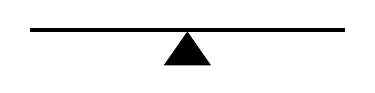
\begin{tikzpicture}
\draw[ultra thick](-2,1) -- (2,1);
\fill[black] (0,0.98) -- (-0.3,0.55) -- (0.3,0.55);
\end{tikzpicture}
\caption{Balanced question}
\label{balanced}
\end{figure}

But as we all know, sometimes questions are biased. For example, the speaker might take one answer to be more likely than another. This leads to an imbalance among the propositions, as in \figref{unbalanced}.

\begin{figure}
%\hspace{0.3cm}\phantom{$\phi$}\\
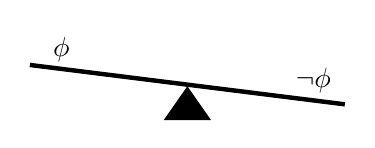
\begin{tikzpicture}[baseline={([yshift={-1ex}]current bounding box.north)}]
\draw[ultra thick](-2,1) -- (2,0.5);
\fill[black] (0,0.73) -- (-0.3,0.3) -- (0.3,0.3);
\node at (-1.6,1.2) {$\phi$};
\node at (1.6,0.8) {$\neg\phi$};
\end{tikzpicture}
\caption{Biased question}
\label{unbalanced}
\end{figure}

There are several interesting questions about this kind of imbalance, including what constitutes the evidence for such an imbalance, whether there are different kinds or different dimensions of tilts, and how can we represent these aspects of meaning.

%\section{Problems for the standard view}

%\subsection{Polar vs. alternative questions}

The existence of biased questions was famously pointed out  by \citet{Bolinger:1978}, who drew attention to the differences between simple polar questions and alternative questions. A polar question like \xref{whetherhelp} is totally normal but an alternative question like \xref{whetherhelpornot} is quite strange, perhaps because the questioner is more interested in the positive answer being true rather than the negative, and this is better expressed by \xref{whetherhelp} than \xref{whetherhelpornot}.

\ea
\ea\label{whetherhelp}
Will you help me?
\ex\label{whetherhelpornot}
Will you help me or not?
\z
\z

Another difference is that polar questions can be conversation starters whereas alternative questions cannot. The sequence in \xref{starter} sounds normal, while that in \xref{nonstarter} sounds odd.

\ea
\ea[]{
Nice to meet you! Do you like to play golf?}\label{starter}
\ex[\#]{
Nice to meet you! Do you like to play golf or not?}\label{nonstarter}
\z
\z

There is also a difference with respect to question complementizers. It seems that embedded polar questions introduced by \textit{if} correlate with simple polar questions, while those introduced by \textit{whether} correlate with alternative questions. Thus, the scenario in \xref{willyoumarryme} is more naturally reported as \xref{ifmarry} than \xref{whethermarry}. 

\ea[]{
John asked Mary: ``Will you marry me?''
}\label{willyoumarryme}
\ex[]{
John asked Mary if she would marry him
}\label{ifmarry}
\ex[?]{
John asked Mary whether she would marry him
}\label{whethermarry}
\z

%John asked Sue if she would marry him is fine, but John asked Sue whether she would marry him seems to indicate that John is neutral about both possibilities, which in this case would make the question sound odd.
Bolinger suggests that the complementizer \textit{whether} is used when the speaker, having already considered the alternative possibilities, is trying to dispassionately gain information about them. We add that this corresponds to our intuition that the use of \emph{whether} in \xref{whethermarry} indicates that John thinks a negative answer is a serious possibility, at least as likely as the positive answer.
%seems to suggest that the subject has no preference with respect to the positive and the negative answer. The complementizer \textit{if}, on the other hand, does not seem to have this inference. %\textcolor{blue}{[DG: My intuition is that the asymmetry here isn't nearly as sharp as for the matrix polar question vs. alternative question. In fact, I think \xref{whethermarry} is basically fine. There is perhaps an intuitive difference, but I wouldn't say that ``whether" conveys that John has ``no preference". It might be that ``whether" conveys that John thinks a negative answer is a serious possibility, though not more likely than the positive answer. Perhaps it conveys that the two answers are equally possible, while ``if" perhaps only draws attention to the positive answer (but doesn't necessarily mean that John is ``biased" for the positive answer).]}

So we see that simple polar questions can highlight one option, while alternative questions highlight both options. We can then ask whether alternative questions are neutral. But as \citet{biezma2019alternative} shows, alternative questions are not neutral. They come with what Biezma calls a `cornering effect': The hearer is forced to give an answer. The question in \xref{marryornot} sounds like it is the last of a series of questions to which the speaker has not gotten a proper answer.

%****DG: I removed the following footnote. This distinction is addressed to a certain extent by Biezma & Rawlins 2017, and Beltrama et al. 2020, who refer to exs like these as "Complement Alternative Questions". Perhaps we'll want to include some discussion of this too, and if so, I can come back and add it. 
%\footnote{This cornering effect seems not to be always present. Consider the following exchange.

%\ex.\label{evenoddexhange}
%\a.[A:] I'm thinking of a number between 1 and 10. Guess which!
%\b.[B:] Is it even or odd?

%Given that a number is either even or odd, B's question is equivalent to an alternative question. However, the question does not have to be read as ``cornering'' A in anyway. \textcolor{blue}{[DG: I thought the cornering effect was only for ``negative alternative questions", which is when the second disjunct is always the negation of the first, e.g. ``or not" or ``or isn't it", etc.]}}

\ea \label{marryornot}
Will you marry me or not?
\z


Let us look at negated questions and the uses of antonyms. Assuming that a bridge is either closed or open, the standard view on questions would assign all of the following sentences the same meaning, namely $\{o, \neg o\}$, where $o$ stands for the bridge is open and $\neg o$ for the bridge is not open, i.e. closed.

\ea\label{bridgequestions}
\ea
Is the bridge open?\label{whetheropen}
\ex \label{openornot}
Is the bridge open or not?
\ex
Is the bridge open or closed?
\ex \label{closed}
Is the bridge closed?
\ex \label{closedornot}
Is the bridge closed or not?
\z
\z

However, the choice of the expression clearly matters \citep{vanrooysafarova2003polar, bustamente2012real, roelofsengool2010disjunctive, trinh2014how}.
In a context where the speaker needs to get to the other side of the river and wants the bridge to be open, and there is no contextual indication as to whether or not it is open, the questions in \xref{bridgequestions} are ranked in the order of most to least appropriate. %, with \xref{whetheropen} being the most appropriate and \xref{closedornot} being the least appropriate. %\textcolor{blue}{[DG: This depends on what else has been said in the context, right? If an interlocutor claims the bridge is closed, and then does or says something to imply it is not closed, the speaker who needs to get to the other side and wants the bridge to be open would then nevertheless find \xref{closedornot} to be most natural, or at least as natural as \xref{whetheropen}.]}

Similarly, in a context where the speaker needs to throw an even number, the utterance in \xref{dice} would be most appropriate with the leftmost choice (\textit{even}) and least appropriate with the rightmost choice (\textit{odd or not}). %\textcolor{blue}{[DG: Suppose the speaker needs an even, but steadfastly believes that their luck is cursed, and therefore an odd number is almost certain. Then ``odd'' is most natural. This comment and my previous comment both are just highlighting the fact that bias has multiple possible sources, as is already mentioned in the chapter above.]}

\ea\label{dice}
I don't dare to look! Is the number even  / $^{?}$even or not / $^{??}$even or odd / \#odd / \#\#odd or not?
\z

However, in both preceding examples, further additions to context can change these intuitions. For example, suppose that in \xref{bridgequestions}, the speaker wants the bridge to be open, but their interlocutor has just indirectly implied that the bridge is closed. In that case, \xref{closed} is most natural. Or suppose the interlocutor ambiguoulsy implies first that it is closed, and then that it is not closed. In that case, \xref{closedornot} would be most natural, despite that the speaker wants the bridge to be open. As for \xref{dice}, suppose the speaker needs an even, but steadfastly believes that their luck is cursed, and therefore an odd number is almost certain. Then asking the question with \textit{odd} is most natural. What this shows is that the contextual factors affecting which question form is most natural are  influenced by multiple competing factors. %All of this shows how sensitive to context the naturalness of the varying forms are. 

How can we differentiate between question meanings so that we can describe their different uses?  Obviously the truth conditional content offered by the theories discussed above does not suffice. We have to look at how these truth conditions are expressed formally. One idea that has been proposed is that different kinds of questions introduce different kinds of discourse referents (DR) (see \citealt{krifka2013} for the role of propositional discourse referents in responses). 

\ea\label{DRs}
\ea \label{rain} 
``Is it raining?'' \hfill $\leadsto$ DR: `it is raining'
\ex\label{notrain}
``Is it not raining?'' \hfill $\leadsto$ DR: `it is not raining'
\ex\label{rainornot}
``Is it raining or not?'' \hfill $\leadsto$ DR: `it is raining', `it is not raining'
\z
\z

As a consequence, these questions would have different discourse potentials. There are other proposals, such as  \citet{roelofsengool2010disjunctive}, which makes it possible to ``highlight'' one of the propositions, leading to a more complex semantic representation. Theories also exist which say the meaning of questions does not have to be balanced. These allow for a monopolar interpretation of questions. Hamblin's semantics, for example, allows for \xref{rain} to denote the set contain only one proposition, namely the proposition that it is raining. The question in  \xref{notrain} would denote the set containing only the proposition that it is not raining. The set denoted by the alternative question in \xref{rainornot} would contain both of these propositions. This is different from the assertion, which is just the proposition, not a set containing the proposition \citep{vanrooysafarova2003polar}.

In commitment space semantics \citep{krifka2015bias}, there is also a way to differentiate between the cases in \xref{DRs}. We assume the common ground, or ``commitment space'', represented by $C$, to be a set of information states, or ``commitment states'', represented by $c$. Each commitment state is a set of possible worlds. The root of C, represented as $\sqrt{C}$, is the set of ``largest'' commitment states, so to speak. %\textcolor{blue}{[DG: In the last draft this said ``smallest'', but I think it should be ``largest'', please double check.]}

\ea\label{rootC}
$\sqrt{C} = \{c \in C \mid \neg\exists c' \in C [c \subset c']\}$
\z

In case of an assertion, say of the proposition that it is raining, represented as $r$, the commitment space C is updated so that it contains only commitment states which entail $r$. 

\ea\label{assertioncommitment}
$C +$ `it is raining' $= \{c \in C \mid c \subseteq r\}$
\z

Questions differ from assertions in that they do not change $\sqrt{C}$, the root of the commitment space. 

\ea\label{questioncommitment}
\ea\label{positivequestioncommitment}
$C +$ `is it raining?' $= \sqrt{C} \cup \{c \in C \mid c \subseteq r\}$
\ex\label{negativequestioncommitment}
$C +$ `is it not raining?' $= \sqrt{C} \cup \{c \in C \mid c \subseteq \neg r\}$
\ex\label{alternativequestioncommitment}
$C +$ `is it raining or not?' $= \sqrt{C} \cup \{c \in C \mid c \subseteq r \vee c \subseteq \neg r\}$
\z
\z

In other words, questions do not add information. Instead, they restrict the continuation of the discourse. As shown in \xref{positivequestioncommitment} and \xref{negativequestioncommitment}, the ``positive'' and the ``negative'' simple polar question restricts $C$ to those $c$ which entail $r$ and $\neg r$, respectively. This is intended to represent the fact that the speaker wants to see if the discourse can continue with the information that it is raining, in the first case, or with the information that it is not raining, in the second case. The alternative question, as shown in \xref{alternativequestioncommitment}, has a yet different meaning from the two simple polar questions.  

Note, however, that this approach would still not capture the distinction between \xref{openornot} and \xref{closedornot}, reproduced below in \xref{openornot2} and \xref{closedornot2}.

\ea\label{openornot2}
Is the bridge open or not?
\ex\label{closedornot2}
Is the bridge closed or not?
\z

The general question, then, is how to represent polar questions properly to capture their different uses.

We now turn to the topic of negation in polar questions \citep{bolinger1957interrogative, Ladusaw:1979, Ladd:1981}. \citet{Ladd:1981} discusses polar questions such as those in \xref{negationquestions}. 

\begin{exe}\label{negationquestions}
\ex\label{lownegation} 
Is it not raining?
\ex\label{highnegation}
Isn't it raining?
\end{exe}

These questions differ with respect to where syntactic negation is. In \xref{lownegation}, it is low, below the subject, while in \xref{highnegation} it is high, above the subject. The low negation question seems to implicate that the speaker wants to be informed as to whether the proposition that it is not raining is true. The high negation question, on the other hand, seems to indicate that the speaker is already inclined to assume that it is raining and wants to confirm this belief.

\citet{Ladd:1981} assumes that high negation questions are actually ambiguous, with both ``outer" and ``inner" interpretations. %Specifically, they allow for a ``low'' interpretation. 
He claims the ambiguity can be resolved by the presence of polarity items like \textit{too} and \textit{either}, which disambiguate the question toward the outer and inner readings respectively. %, or a negative polarity item such as \textit{neither}, which disambiguates the question towards the low reading. %Examples are given in \xref{tooeither}

\begin{exe}\label{tooeither}
\ex\label{too}
Isn't Jane coming too? \hfill $\rightarrow$ outer interpretation
\ex\label{either}
Isn't Jane coming either? \hfill $\rightarrow$ inner interpretation
\end{exe}

A prominent analysis of these facts is proposed by \citet{romerohan2004negative}. %Han:2002a
This analysis assumes a \textsc{verum} operator, whose meaning is a conversational version of the adverbial \textit{for sure}, and whose occurrence is associated with a syntactically preposed high negation. We have the following form-meaning pairs, where $p$ stands for the proposition that Jane is coming. Notice that negation can scope either below or above the \textsc{verum} operator.

\begin{exe}\label{hanromero}
\ex\label{hanromerolowneg}
Is Jane not coming? \\= \textsc{whether}($\neg p$) = $\{\neg p, \neg\neg p\}$ = $\{p, \neg p\}$
\ex\label{hanromerohighnegeither}
Isn't Jane coming (either)? \\ = \textsc{whether}(\textbf{verum}($\neg p$)) = $\{$\textit{for-sure}($\neg p$),  $\neg$\textit{for-sure}($\neg p$)$\}$
\ex\label{hanromerohighnegtoo}
Isn't Jane coming (too)? \\ = \textsc{whether}($\neg$\textbf{verum}($p$)) = $\{$$\neg$\textit{for-sure}($p$), \textit{for-sure}($p$)$\}$
\end{exe}

Romero and Han propose that \textsc{verum} is also present when the question contains the adverb \textit{really}. Thus, \xref{hanromeroreally} ends up having the same meaning as \xref{hanromerohighnegtoo}.

\ea\label{hanromeroreally}
Is Jane really coming?\\
= \textsc{whether}(\textbf{verum}($p$)) = $\{$\textit{for-sure}($p$), $\neg$\textit{for-sure}($p$)$\}$
\z

A similar approach is adopted by \citet{krifka2015bias}, which assumes a commitment operator $\vdash$ that is present in both assertions and questions, and negation can scope either below or above that operator.

\begin{exe}\label{krifkacommitmentoperator}
\ex
$C +$ `is Jane not coming?' = $\sqrt{C} \cup C +$ [Addressee $\vdash$ $\neg p$]\\
$\leadsto$ the speaker is checking whether the addressee is committed to $\neg p$
\ex
$C +$ `isn't Jane coming?' = $\sqrt{C} \cup C +$ $\neg$[Addressee $\vdash$ $p$]\\
$\leadsto$ the speaker is checking whether the addressee is not committed to $p$
\end{exe}

So, there is a wide array of syntactic profiles available for polar question formation: high and low negation, the presence or absence of adverbials like \textit{really}, and also, the presence or absence of bias inducing expressions such as negative polarity items (NPIs). \tabref{tab:1} presents a fine-grained list (probably non-exhaustive) of relevant phenomena (see also the bias profiles discussed in \citealt{gartnergyuris2017delimiting}).

\begin{table}[t]
\fittable{
\begin{tabular}{lll}
\lsptoprule
Example & Abbreviation & Label\\
\midrule
Is it raining? & PQ & positive question\\
Is it not raining? & NQ & negative question\\
Isn't it raining? & HPQ & high negated positive question\\
Isn't it not raining? & HNQ & high negated negated question\\
Is it really raining? & RPQ & \textit{really} positive question\\
It is really not raining? & RNQ & \textit{really} negated question\\
IS it raining? & FPQ & focused positive question\\
IS it not raining? & FNQ & focused negated question\\
Is it REALLY raining? & FRPQ & focused \textit{really} positive question\\
Is it REALLY not raining? & FRNQ & focused \textit{really} negated question\\
It is raining? & DPQ & declarative positive question\\
Is it raining?? & IPQ & incredulity positive question\\
Is it raining or not? & APNQ & alternative question with negation\\
Is the bridge open or closed? & AAntQ & alternative question with antonyms\\
Do you have any potatoes? & npiPQ & positive question with polarity item\\
\lspbottomrule
\end{tabular}
}
\caption{Polar question varieties} \label{tab:1}
\end{table}

Coming back to the topic of negation in questions, one promising approach is to look at contextual features. This goes back to \citet{buringgunlogson2000positive}, which assumes three levels of contextual evidence with respect to the prejacent of a polar question: positive, neutral, and negative. The generalization in \tabref{buringgunlogsongeneralization} is established. 
%\textcolor{blue}{[DG: I'm doubtful that we can get people to adopt the terminology and abbreviations in Table 1.Given that, I think the only reason to  introduce systematic abbreviations here is if we ourselves can consistently use them in the rest of the chapter. But in the following, we display and discuss plots from a few different experiments by other researchers who each have their own different abbreviations, including already ``PPQ" in the next table. So, I suggest that we remove Table 1.]} %Lots of people have worked on this topic now and there is no agreed upon terminology, let alone abbreviations. 

\begin{table}
\begin{tabularx}{\textwidth}{lCCc}
  \lsptoprule
\multirow{2}{*}{contextual evidence} & \multirow{2}{*}{PPQ} & \multicolumn{2}{c}{HPQ} \\
\cmidrule{3-4}
 & {} & high reading & low reading \\
   \midrule
positive & \ding{51} & \ding{55} & \ding{55}\\
neutral & \ding{51} & \ding{51} & \ding{55}\\
negative & \ding{55} & \ding{51} & \ding{51}\\
  \lspbottomrule
\end{tabularx}
\caption{\quotecite{buringgunlogson2000positive} generalization} \label{buringgunlogsongeneralization}
\end{table}

\largerpage[2]
The contextual evidence is ``positive'' if it supports the prejacent, ``neutral'' if it neither supports nor speaks against the prejacent, and ``negative'' when it speaks against the prejacent. Thus, even PPQs are not neutral, in the sense that there are contexts where they cannot be used, namely those with negative evidence. Note that \citet{buringgunlogson2000positive} take HPQ with a low negation to mean the same as NQ. Thus, \xref{hpqlow} and \xref{nq} would be equivalent in this approach.

\ea
\ea\label{hpqlow}
Isn't Jane coming either?
\ex\label{nq}
Is Jane not coming either?
\z
\z

The first experimental work on this topic is done by \citet{roelofsen2013}. This is a rating experiment, which contrasts prior speaker's belief (SB) with positive, neutral, and negative contextual evidence (CE). The experiment yields interesting results about the different uses of positive, high negation, and low negation questions as presented in \figref{pic:123}.
%\textcolor{blue}{[DG: I haven't read this paper, and I guess I need to. The results in (24) and (25) make no sense to me. Either I've misunderstood or there was a problem with the stimuli. Note also that we don't actually discuss this data below, which makes me wonder if we should include these plots. It seems the main reason for mentioning this paper is to discuss the preference rules and OT below, maybe we could just do that directly.]}

\begin{figure}
\subfigure[PPQs]{
\includegraphics[width=.45\textwidth]{figures/Roelofsen-PPQ.pdf}
}
\subfigure[HNPQ]{
\includegraphics[width=.45\textwidth]{figures/Roelofsen-HNPQ.pdf}
}
\subfigure[LNPQ]{
\includegraphics[width=.45\textwidth]{figures/Roelofsen-LNPQ.pdf}
}
\caption{\quotecite{roelofsen2013} experimental results}
\label{pic:123}
\end{figure}


These uses were described in terms of various preference rules. An example of such a rule is ``ask only if needed''. According to this rule, there is no need to ask any question if speaker's belief and contextual evidence coincide. Another rule is ``avoid reversing processes'', which says that it would be strange to ask whether $\neg p$ is true when the speaker's belief or the contextual evidence supports $p$. Yet another rule is ``use the least marked form'', which would prefer a positive question to a negative or an alternative question, for example. We note that these rules resemble constraints in bidirectional optimality theory (OT) in pragmatics, hence raise the question whether bidirectional OT should be employed in analyzing biased questions. We believe this perspective is promising.

It has become consensus to assume three levels -- positive, neutral, negative -- for both contextual evidence and prior speaker's belief, or ``evidential bias'' and ``epistemic bias'', which are terms proposed by \citet{sudo2013biased} which have gained some currency. We could let SB stand for prior speaker's belief and CE for contextual evidence, and use $+$, $0$ and $-$ to represent the three levels positive, neutral, and negative. %Furthermore, we could adopt the convention of placing. 
Bias profiles of questions could then be represented more succinctly. For example, [SB$-$, CE$+$] is a question with negative prior speaker's belief and positive contextual evidence, and [SB$0+$, CE$-$] would be a question with neutral or positive prior speaker's belief and negative contextual evidence. If we adopt the convention of placing the value for SB to the left of that for CE, the profiles can be represented even more economically. Thus, [SB$-$, CE$+$] can be shortened to [$-$/$+$] and [SB$0+$, CE$-$] to [$0+$/$-$]. %\textcolor{blue}{[DG: It looks like maybe we get some use of these abbreviations some of the tables below; maybe we should introduce those abbreviations there.]} 

\citet{domaneschi2017bias} present further experimental results. Tests were conducted on high negation questions (HiNQ), low negation questions (LowNQ), positive question (PosQ), and positive question with \textit{really} (ReallyPosQ). The object languages were English and German. Participants were given a selecting task, where they had to pronounce their option. The main results are presented in \figref{fig:chart23}. %\textcolor{blue}{[DG: With this data as well, we're not really discussing it. Perhaps that is fine, and the idea here is just to provide the reader with the results themselves. But then we need to explain the condition labels on the X axis. If we decide to keep these plots in here, I am happy to add explanations for the condition labels.]}

\begin{figure}
% \begin{subfigure}{0.43\textwidth}\centering
\includegraphics[height=.45\textheight]{figures/Domaneschi-1.pdf}
%\caption{\color{red}{Please provide a caption}}
%\label{fig:chart2}
% \end{subfigure}
% \begin{subfigure}{0.41\textwidth}\centering
\includegraphics[height=.45\textheight]{figures/Domaneschi-2.pdf}
%\caption{\color{red}{Please provide a caption}}
%\label{fig:chart3}
% \end{subfigure}
\caption{\quotecite{domaneschi2017bias} experimental results}
\label{fig:chart23}
\end{figure}

A recurring question is whether syntactically high negation questions (HPQs) are semantically ambiguous. \citet{Ladd:1981} claims that they are; \citet{sailor2012remarks, anderbois2019, goodhue2022} all argue that they are not. It should be pointed out, however, that Sailor's data can be accounted for by assuming that for English, HPQs are ambiguous while NQs are not, and for German, the opposite is the case. %\textcolor{blue}{[DG: I'm not sure what is meant by this claim. In my paper, I make a concerted effort to show that the data speaks against the existence of an ambiguity in American English HPQs.]}

\ea English
\ea Isn't there a train in the early morning? \hfill $\neg Qp$ / $Q\neg p$
\ex Is there no train in the early morning? \hfill $Q \neg p$
\z

\ex German
\ea Gibt es hier nicht einen Zug am Morgen? \hfill $\neg Qp$
\ex Gibt es hier keinen Zug am Morgen? \hfill $Q\neg p$ / $\neg Qp$
\z
\z

How can we explain this difference between English and German? Suppose we say that in the [SB$+$, CE$-$] scenario, the wide-scope negation reading is the best. If we then assume that in German this wide-scope interpretation can also be expressed by a syntactically low negation, we can explain why there is more uses of this option in German.

The interesting issue here, therefore, is whether there are different readings of high negation questions and low negation questions. 

\citet{sudo2013biased} looks at the Japanese counterparts of positive questions (PQs), high negation questions (HQs), and low negation questions (NQs). 

\ea
\gll Mary-ga kita $\{\emptyset$ / no / desho$\}$\\
Mary-NOM came\\ 
\glt `Did Mary come' \hfill PQ 
\ex
\gll doko-ka nihon-shoku nai?\\
where-\textsc{ka} Japanese-food not.exist\\
\glt `Isn't there some Japanese restaurant?' \hfill HQ
\ex
\gll doko-mo nihon-shoku nai?\\
where-\textsc{mo} Japanese-food not.exist\\
\glt `Isn't there any Japanese restaurant?' \hfill NQ
\z

Sudo treats epistemic and evidential bias, at different levels, as features which can be combined in different ways as presented in \tabref{figtab:chart45}. \citet{gyuris2017new} looks at three different types of polar questions in Hungarian as presented in \tabref{figtab:chart6}.

\begin{table}
% \includegraphics[width=.5\textwidth]{figures/Sudo-1.pdf}
\caption{\quotecite{sudo2013biased} taxonomy}
\label{figtab:chart45}
\begin{tabularx}{\textwidth}{XXXc}
\lsptoprule
 Question type & Epistemic &  Evidential & Short\\
 \midrule
 PQ            & none      &  not negative &  --0+/0+\\
 HQ            & positive  &  not positive & +/--0\\
NQ             &  positive & neutral        & +/0\\
\lspbottomrule
\end{tabularx}
\end{table}

\begin{table}
% \includegraphics[height=.5\textheight]{figures/Gyuris-1.pdf}
\caption{\quotecite{gyuris2017new} taxonomy}
\label{figtab:chart6}
\fittable{
\begin{tabular}{lccc}
\lsptoprule
                                  & -e-interrogative &  $\wedge$-interrogative  & $\wedge$-declarative\\
                                  \midrule
Neutral information question, (11)& {\langscicheckmark} & {\langscicheckmark} & {\langscicross}\\
Grounding question, (12)          & {\langscicross}     &\%                   & {\langscicheckmark}\\
Indirect Request                  & {\langscicross}     &  {\langscicheckmark}& {\langscicross}\\
Indirect offer, (14)              & {\langscicheckmark} &  {\langscicheckmark}& {\langscicross} \\
 Conversation  starter, (15)      & {\langscicross}     &  {\langscicheckmark}& {\langscicross}\\
Pedagogical question              & {\langscicheckmark} & {\langscicheckmark} & {\langscicross}\\
Monological question              & {\langscicheckmark} & {\langscicheckmark} & {\langscicross}\\
Exam question, (18)               & {\langscicheckmark} & {\langscicheckmark} & {\langscicross}\\
Rhetorical question, (19)         & {\langscicheckmark} & {\langscicheckmark} & {\langscicross}\\
\lspbottomrule
\end{tabular}
}
\end{table}

\begin{table}
% \includegraphics[height=.17\textheight]{figures/Gyuris-2.pdf}
\caption{\quotecite{gartnergyuris2017delimiting} bias profiles}
\label{figtab:chart7}
 \begin{tabularx}{.8\textwidth}{Xcc}
 \lsptoprule
 Question type & Speaker belief & Current evidence\\
 \midrule
  ePQ          &                 &0                        \\
 $\wedge$PQ          &                 &0, for some speakers --  \\
 $\wedge$DPQ         &                 &+                        \\
 eHQ           &   +             &0                        \\
 $\wedge$HQ          &   +             &--0                      \\
 $\wedge$NQ          &   +             &--                       \\
 $\wedge$DNQ         &                 &--                       \\
 \lspbottomrule
  \end{tabularx}
\end{table}

\citet{gartnergyuris2017delimiting} look at possible bias profiles (see \tabref{figtab:chart7}). There are $7 \times 7 = 49$ possible SB/CE combinations. When we consider the three types of questions (PQ, HQ, NQ), we end up with $7^3 \times 7^3 = 117649$ possibilities, which is an astonishing number due to combinatorial explosion. But one can reduce the number of possibilities by certain general principles. %\textcolor{blue}{[DG: Like what?]}
For example, a principle of Markedness could favor non-negated questions over negated ones so that they are also used for neutral questions (cf. also \citealt[230]{trinh2014how}). 

Let us now turn to the topic of NPIs in questions \citep{Ladusaw:1979, Kadmon:1993, krifka1995semantics, vanRooy:2003}. It has been observed that NPIs do not occur in declarative questions. Since declarative questions presumably have a [$-0+$/$+$] profile, in case of rising contour, or a [$-$/$+$] profile, in case of incredulity contour, questions with NPIs must have a [*/$-$0] profile. Questions with strong idiomatic NPIs (i.e. minimizers) appear to have a [$-$/$-0$] profile, meaning their use requires that the speaker not believe and the context not have evidence for the prejacent.

\ea
\ea
Did John do anything to help?
\ex
Did John lift a finger to help?
\z
\z

\citet{asherreese2005negative} account for NPIs in questions by assuming that such questions actually come with a negated assertion, which is what licenses the NPI. Another way to explain the felicity of NPIs in questions is by appealing to the fact that a question denotes a set containing a proposition and its negation, and it is the negated proposition which licenses the NPIs. The unacceptability of NPIs in declarative questions can then be explained by saying that these questions are monopolar: they denote sets containing only one proposition. \citet{guerzoni2014} account for the distribution of NPIs in questions by claiming that many questions contain covert disjunction with a covert negation that licenses the NPI. On this view, it could be argued that declarative questions fail to license NPIs because they lack covert disjunction and negation. 

\citet{krifka1995semantics} and \citet{vanRooy:2003} propose that NPIs in questions create a more equal distribution of the likelihood of both options by way of widening the meaning of the NP complement. Thus, \textit{potatoes} in \textit{any potatoes} would denote a superset of \textit{potatoes} in \textit{some potatoes}. Strong NPIs would increase the chance of the positive answer being true, and this is a strategy for showing preference for the negative answer. It is, however, not clear how to represent the bias which comes about by way of (strong) NPIs with the features that we have discussed. %\textcolor{blue}{[DG: Should we also cite Guerzoni \& Sharvit here about NPIs in questions?  I haven't read the paper closely, perhaps someone with more expertise on NPIs in Qs has an opinion...]}

We believe that a distinction has to be made within the category of contextual evidence (CE). Specifically, we need to differentiate between CE which is factual and CE which is infered from what the addressee says. %\textcolor{blue}{[DG: This and the following idea about assertions are both very interesting, but also terse enough that I'm not sure what to make of them. Why does this distinction have to be made? Do we think it affects what the speaker bias profile of the question can be? Perhaps it does, but I think it requires demonstration.]}

\ea Factual
\ea A: Coming in with a dripping raincoat
\ex B: Is it really raining outside?
\z
\z

\ea Addressee's belief
\ea A: The rain is bothering me!
\ex B: Is it really raining outside?
\z
\z

This leads us to the question of when an assertion is biased. Presumably, an assertion is biased if the speaker's belief supports the asserted proposition, there is no contextual evidence against it, but the addressee does not believe it yet. We can enrich our feature notation by placing the addressee's belief in brackets.

\ea
It is raining \hfill [$+$/$0+$] or [$+$/$0+(-0)$]
\ex
It isn't raining \hfill [$-$/$-0$] or [$-$/$-0(0+)$]
\ex
Really, it is raining \hfill [$+$/$0+(-)$]
\z

Other relevant topics include in-situ wh-question \citep{biezma2019alternative}, assertions with question tags, and miratives \citep{delancey1997mirativity, bustamente2012real}. 

Last but not least, we would like to emphasize the importance of prosody. In this connection, \citet{Bartels:1999} should receive mention. We would draw attention to the discussion on ``falling'' declarative questions, i.e. those that are not marked by rising contour. Other works on prosody and bias include \citet{gricesavino2003map}, \citet{kugler2004dialectal}, and \citet{arnhold2021}. 

\section{The contributions to this volume}

In their chapter \textit{Biased questions and modal ranking}, Alda Mari and Anastasia Giannakidou point out that questions share a semantic feature with epistemic modals: They are non-veridical in the sense that they do not entail that their prejacent proposition $p$ is true. The authors suggest that questions with negative and positive bias lie on a continuum between regular questions and assertions, and that they share this property with weak and strong epistemic modals that modify assertions. Both questions and epistemically modified statements require that the modal base of the speaker contains both $p$ and $\neg p$ worlds (the ``nonveridicality axiom of modals and questions''). But questions and epistemically modified statements differ insofar as only the latter have truth conditions and can be said to be true or false. The authors discuss three empirical domains. First, \textit{really}-questions are analyzed as marking a genuine interest of the speaker and having a negative bias. They provide an account of \textit{really} in which this adverb points to a different ranking of propositions between the assumptions of the speaker and evidence of the context, with reference to experimental work on \textit{wirklich} in German. They show that negatively biased questions ask for stronger confirmation; a response like \textit{I think so} is felt to be insufficient. The second domain are questions with high negation and low negation with a positive bias, which are related to assertions with the strong modal \textit{must} that also expresses a positive bias. The third domain are \textit{reflective} or \textit{conjectural} questions marked with weak epistemic modals, such as \textit{might}. They observe that the modals must be weak, and argue that they widen the modal base, enlarging the range of possibilities, thus unearthing remoter ways in which a proposition may be true. As for assertions, the authors suggest that they are only added into the common ground when not modalized.    


In her chapter, \textit{Evidential bias across clause types}, Beste Kamali compares English rising declarative questions, known to express a positive bias towards their proposition, with a polar question type in Turkish. In this language, polar questions are always marked by a particle \textit{\textsc{mi}} that is attached to a constituent of the sentence, then often marking the focus of the question, or after the (typically final) finite verb of the sentence, indicating a polar question without focus. However, when \textit{\textsc{mi}} attaches to the direct object, focus may project to the whole sentence. There are subtle differences between such sentences and sentences where \textit{\textsc{mi}} is attached to the final verb. In particular, the object-\textit{\textsc{mi}} sentences have a reading that has a similar bias to English rising declarative questions, insofar as they also require a positive evidential bias. However, a careful examination in a battery of tests reveals interesting differences: First, object-\textit{\textsc{mi}} questions are classified as ``questions'' in the object language, different from English (cf. \textit{One question remains: Did Ali make dinner?} / \textit{\#Ali made dinner?}). They do not allow for modal adverbials, different from English (cf. \textit{You certainly made dinner?}). And they can be embedded by rogative predicates, again different from English (*\textit{She asked Ali made dinner?}).  Hence, object-\textit{\textsc{mi}} questions achieve their positive bias in ways quite different from English declarative questions. According to the proposed analysis, they both are monopolar, in contrast to regular polar questions and verb-final \textit{\textsc{mi}}-questions, which are analyzed as bipolar. Their differences derive from the fact that they are syntactically and semantically different clause types. The author also draws in evidence from Hungarian and Japanese that show similar question types as Turkish object-\textit{\textsc{mi}} questions. 


In their chapter, \textit{The contribution of intonation in the conveyance of question bias}, Riccardo Orrico, Cristel Portes, Mariapaola D'Imperio provide a comprehensive overview of the role of intonation in the expression of question bias. They begin with a review of the literature on intonation patterns and the different dimensions of meaning they can express. This review is followed by a discussion of two recent experimental studies conducted by the authors themselves. Throughout the chapter, the authors address three main questions about the relationship between phonetic cues and speaker meaning: the kinds of meanings that can be expressed by intonation, the intonational cues that convey these meanings, and the degree of variation within the linguistic population. After a general overview, they provide a detailed comparison of the means used by Italian and French speakers to express question bias. They argue that the way in which meaning is encoded in intonation patterns is not universal. Their study shows that different languages have their own specific cues to express specific meanings.  

In their chapter, \textit{Negative Polar Questions in Russian: Question bias and question concern}, Sophie Repp and Ljudmila Geist study the appropriateness conditions of yes--no questions containing the particles \textit{razve} and \textit{neu\v{z}eli}, both of which can be translated as \emph{really}. In their analysis, they distinguish between the bias profile of a question and the \textit{question concern}. The \textit{bias profile} is defined by the question's \textit{epistemic} and \textit{evidential} bias \citep[following][]{s3budo201iased}, where the former refers to the speaker's prior beliefs and the latter to contextual evidence that may or may not conflict with the speaker's beliefs. By \textit{question concern} they refer to the purpose of checking or rejecting the prejacent of a question, or its negation. Repp and Geist assume that the appropriateness of different types of polar questions depends on their bias profile and their concern. They demonstrate the usefulness of this asumption for polar questions in English, and then extend the analysis to polar questions in Russian with or without particles \textit{razve} and \textit{neu\v{z}eli}. Repp and Geist show that polar questions with \textit{razve} and \textit{neu\v{z}eli} do not differ in their bias profile but in their ability to check the truth of the proposition which is favoured by the question's epistemic bias. Repp and Geist support their analysis by a corpus study and two experimental investigations. They further provide a semantic explanation for the difference between \textit{razve} and \textit{neu\v{z}eli} in terms of their consistency with inner and outer negation.

In their chapter, \textit{Bias in Tag Questions}, Corey Bill and Todor Koev study constructions consisting of a VP-eliptical yes/no question which is ``tagged'' onto an ``anchor'' declarative sentence of the opposite polarity, as exemplified by \textit{it's raining, isn't it?} and \textit{it's not raining, is it?}. It has been observed that tag questions give rise to the inference that the speaker is ``biased'' toward the anchor, i.e. that she believes the proposition it expresses to be true. Bill and Koev propose to describe such biases in terms of two parameters: (i) whether they are weak or strong, and (ii) whether they are optional or obligatory. They devise diagnostics to test these distinctions, and advance an analysis to derive the observations from syntactic and phonological properties of tag questions.

In their chapter, \textit{Contextual Bias and the Landscape of Mandarin Polar Questions}, Yurie Hara and Mengxi Yuan discuss \textit{ma}-questions and A-not-A questions in Mandarin Chinese. They present the following observations: (i) positive \textit{ma}-questions can be used in either neutral or positively biased contexts; (ii) negative \textit{ma}-questions can only be used in negatively biased contexts; (iii) A-not-A questions can only be used in neutral contexts. They then argue that it is contextual bias, not speaker's bias, which is instrumental for an analysis of this distribution. The concept of ``contextual bias'' is defined in terms of subjective probability and \citeauthor{farkasbruce2010reacting}'s (\citeyear{farkasbruce2010reacting}) Table model.

In their chapter, \textit{What can Cantonese sentence-final particles tell us about rhetorical questions?}, Angelika Kiss, Roger Yu-Hsiang Lo, and Justin R. Leung discuss three kinds of questions: (i) information seeking questions (ISQ), (ii) rhetorical question with empty set answers (RQ–), and (iii) rhetorical questions with non-empty set answers (RQ+). It uses the framework of inquisitive semantics to argue that these are in fact natural classes in terms of informativity and speaker's commitment. Moreoever, ISQ and RQ– make up a subclass in this three membered group. An perception experiment is then presented whose result shows that the semantic distinctions are also reflected prosodically in Cantonese, specifically in distinctions with respect pitch contour and length of the final sentence particle.

In his chapter, \textit{A note on bias and polarity in Vietnamese}, Tue Trinh discusses the distribution of two types of NPIs across two types of polar questions. NPIs in Vietnamese come in two morphological variants, one simple and one complex. Among polar questions in this language, Trinh distinguishes between yes/no questions and agreement questions. The observation is that complex NPIs are acceptable in yes/no questions but deviant in agreement questions, and in yes/no questions, complex NPIs give rise to negative bias while simple NPIs do not. The analysis Trinh proposes for this fact assumes that complex NPIs require a covert EVEN in the structure, and that agreement questions contain a covert evidential marker. 


%In their chapter, {\bf Psycholinguistic processing tasks and the study of question bias}, E Jamieson and Vinicius Macuch Silva approach the issues related to biased questions from the experimental perspective. The chapter discusses different theoretical approaches to biased questions, overview of Psycholinguistic investigation on the topic, as well as what data from the experimental studies provide for the ongoing discussion, contrasting with the more traditional introspective data and judgments. In addition, Jamieson and Silva provide concrete suggestions and guidance regarding the aspects of experimental set-up, providing important resources for future researches.

Much of the study on biased questions has been based on the introspective intuition from different languages. In this chapter, \textit{Psycholinguistic processing tasks and the study of question bias}, E Jamieson and Vinicius Macuch Silva provide another dimension: how can we investigate the issues related to biased questions from an experimental perspective? The chapter discusses different theoretical approaches to biased questions, an overview of psycholinguistic investigations on this topic, as well as the contribution of experimental data to the ongoing discussion and understanding of polar questions. In addition, Jamieson and Silva provide concrete suggestions and guidance regarding the aspects of experimental set-up, providing important resources for future researches.


Hungarian interrogatives are marked with a special suffix. In her chapter, \textit{Marking the type of speaker bias: Hungarian \textit{nem-e} interrogatives}, Gyuris examines a particle \textit{nem-e}, which consists of a negation and an interrogative marker. This particle has not been investigated before, and naturally, Gyuris is the first to describe the different characteristics that the particle exhibits, and to a semantic account.  Gyuris first discusses the meaning contribution and the distribution of the canonical question particle \textit{-e}, showing the interaction between its meaning and biases. She then discusses the data on \textit{nem-e}, and reveals that their meaning and distributional pattern reveal cross-dialectal variation: \textit{nem-e} gives rise to the outside negation reading but not inside negation reading, and is incompatible with different types of biases.
After identifying different uses of \textit{nem-e}, Gyuris provides analyses of the particle, which predicts and accounts for their distribution. The chapter is a welcome addition to our understanding of biased questions.


In their chapter, \textit{Children's acquisition of English ``high'' negation: A window into the logic and composition of bias in questions}, Rebecca Woods and Thomas Roeper investigate the production of English nuclear negative tag structures and negative questions, produced by children and adults. They argue that the structures of negative tags and negative questions are distinct, the former being simple speech acts that are complex at the clausal level. The negative questions, on the other hand, involve an interrogative clause, scoped over by metalinguistic negation and a question operator. Woods and Roeper provide a new type of evidence for their analysis, providing making valuable (and novel) empirical contribution to the volume (suggetion)s.

In his chapter, \textit{Everything that rises must converge: Toward a unified account of inquisitive and assertive rising declaratives}, Daniel Goodhue investigates the relationship between rising declarative clauses that are used to ask questions, and those that are used to make assertions. English matrix declaratives with a final rising intonation typical of polar questions are frequently used as a biased question: they convey that there is contextual evidence in favor of the proposition denoted by the declarative. However, some rising declaratives assert the content of the declarative, while raising a second issue. Goodhue offers a unified account of rising declaratives that seeks to explain both of these kinds of uses while positing unitary meanings for clause types and intonations. Achieving this goal depends the view that illocutionary force is not determined by clause type and intonation. Instead, clause type and intonation are proposed to merely constrain what a speaker could intend to do with them; pragmatic inference then plays a key role in enabling an audience to uncover the speaker's illocutionary intention. The proposed account enables a derivation of assertive force. 

\printbibliography[heading=subbibliography,notkeyword=this]
\end{document}
 
\chapter{A feature-based approach to functional left peripheries} \label{ch:2}
\section{Introduction} \label{sec:2introduction}
%\chaptermark{A feature-based approach}
In this chapter, I am going to present the basic assumptions concerning a minimal, feature-based approach to the syntax of functional left peripheries, showing that the proposed analysis applies to various clause types, in each case correctly predicting the surface order of clause-typing elements appearing in combinations. Since the relevant combinations are restricted to embedded clauses in Germanic languages, this chapter will be focusing on subordinate clauses, even though, as will be indicated, the analysis is also applicable to main clauses. In particular, I will be arguing against cartographic approaches, showing that clause-typing elements appearing on functional left peripheries are not in a one-to-one relationship with syntactic features, and the assumption that there are designated projections for the various semantic properties is fundamentally flawed. Instead, I propose that functional left peripheries are as minimal as possible, and multiple projections are generated when the relevant semantic properties cannot be marked in a single projection; whether this is the case is ultimately dependent on the lexical properties of the individual clause-typing elements. To put the analysis into an appropriate context, I am first going to review some previous proposals of relevance: the papers discussed here are not meant to be a representative summary of the state of the art but they are selected analyses that have been particularly influential and/or are of particular interest for the analysis pursued here.

This chapter is structured as follows. Section \ref{sec:2previous} provides an overview of some previous accounts. Section \ref{sec:2introducing} introduces the basic ideas regarding the flexible approach to left peripheries put forward in this book. This basic proposal will be refined with more details in the subsequent sections: \sectref{sec:2interrogatives} discusses embedded interrogatives, \sectref{sec:2relative} discusses relative clauses, and \sectref{sec:2degree} discusses embedded degree clauses. These clauses types will be dealt with in more details in the rest of this book.

\section{Previous accounts} \label{sec:2previous}
\subsection{The problems to be discussed} \label{sec:2problems}
In current minimalist theory, the Complementiser Phrase (CP) is responsible for typing clauses and for encoding finiteness in finite clauses.\footnote{See, for instance, \citet[283]{rizzi1997}, for anchoring finiteness in the CP-system. Note that finiteness is ultimately inherited from the inflectional system (see \citealt{chomskylasnik1977} and \citealt{denbesten1983}). This also means that a clause can be finite without a CP layer, as is the case for English main clause declaratives, which are standardly assumed to be TPs.} Apart from complementisers, various operators can appear in this domain. Consider:

\ea
\ea I wonder \textbf{if} Ralph has arrived. \label{englishif}
\ex I wonder \textbf{whether} Ralph has arrived. \label{englishwhether}
\z
\z

In (\ref{englishif}), the element \textit{if} is a complementiser and it types the subordinate clause as interrogative. In (\ref{englishwhether}), there is no overt complementiser but the operator \textit{wheth\-er} is present. In such cases, it is generally assumed that the zero complementiser types the clause, yet a sound model of the CP-periphery must also clarify the role of the overt operator in (\ref{englishwhether}), especially because its appearance in dialects like Standard English is tied to the absence of the overt complementiser:

\ea[*]{I wonder \textbf{whether if} Ralph has arrived. \label{whetherifch2}}
\z

On the other hand, the CP is not restricted to hosting a single overt element: depending on the particular construction and the dialect, multiple elements may appear in the CP-domain. This is illustrated by (\ref{englishdfc}) for non-standard English and by (\ref{norwegiandfc}) for Norwegian\footnote{The Norwegian data stem from the cross-Germanic survey of \citet[175]{bacskaiatkaribaudisch2018}. Both of the informants marked the sentence in (\ref{norwegiandfc}) as grammatical.}:

\ea \label{dfc}
\ea[\%]{ I wonder \textbf{which book that} Ralph is reading. \label{englishdfc}}
\ex[]{ \gll Peter spurte \textbf{hvem} \textbf{som} likte bøker. \label{norwegiandfc}\\
Peter	asked.\textsc{3sg} who	that liked books\\
\glt `Peter asked who liked books.'}
\z
\z

A proper formal account of the CP-domain must be able to condition when multiple overt elements are allowed and when not. Further, it must be clarified whether the appearance of several overt elements requires multiple CP projections, and in cases where it does, how word order restrictions can be modelled. The generation of multiple functional layers is in principle possible, yet it should be appropriately restricted to exclude the generation of superfluous layers that are empirically not motivated. This question is likewise relevant in cases involving a single overt C-element, since then the question arises whether and to what extent covert elements and phonologically invisible projections are present.

Apart from the exact position of various elements in the CP, their function(s) must also be addressed. For instance, interrogative complementisers regularly encode finiteness as well, imposing finiteness restrictions on the complement TP. Consider:

\ea \label{ifwhether}
\ea[]{I don't know \textbf{if} I should call Ralph. \label{iffinite}}
\ex[]{I don't know \textbf{whether} I should call Ralph. \label{whetherfinite}}
\ex[*]{I don't know \textbf{if} to call Ralph. \label{ifnonfinite}}
\ex[]{I don't know \textbf{whether} to call Ralph.  \label{whethernonfinite}}
\z
\z

\begin{sloppypar}
In (\ref{iffinite}), the complementiser \textit{if} introduces a finite embedded interrogative clause, and as the ungrammaticality of (\ref{ifnonfinite}) shows, it is incompatible with a non-finite clause, suggesting that it encodes finiteness apart from the interrogative property. By contrast, the operator \textit{whether} is compatible with both a finite clause, as shown in (\ref{whetherfinite}), and with a non-finite clause, as shown in (\ref{whethernonfinite}), indicating that the overt marking of interrogativity is not incompatible with a non-finite clause in English. Since \textit{whether} is not specified for finiteness, it should be clear that finiteness is specified by some other element in (\ref{whetherfinite}); the question is whether there is a separate element encoding finiteness in (\ref{iffinite}) as well and, if so, how the restriction of \textit{if} to finite clauses can be explained.
\end{sloppypar}

Finally, the function(s) of various left-peripheral elements must be clarified also because there are some non-trivial combinations in which elements seem to be largely similar, as in the non-standard German example in (\ref{alswie}) below:

\ea
\ea[\%]{\gll Ralf ist größer \textbf{als} \textbf{wie} Maria. \label{alswie}\\
Ralph is taller than as Mary\\
\glt `Ralph is taller than Mary.'}
\ex[]{\gll Ralf ist größer \textbf{als} Maria. \label{als}\\
Ralph is taller than Mary\\
\glt `Ralph is taller than Mary.'}
\ex[\%]{\gll Ralf ist größer \textbf{wie} Maria. \label{wie}\\
Ralph is taller as Mary\\
\glt `Ralph is taller than Mary.'}
\ex[]{\gll Ralf ist so groß \textbf{wie} Maria. \label{wieequat}\\
Ralph is so tall as Mary\\
\glt `Ralph is as tall as Mary.'}
\z
\z

In (\ref{alswie}), the elements \textit{als} and \textit{wie} both seem to mark the comparative nature of the clause, whereby single \textit{als} is the comparative particle in Standard German comparatives, see (\ref{als}), and single \textit{wie} is the comparative particle in equatives, see (\ref{wie}), and in certain dialects also in comparatives, see (\ref{wieequat}). In such cases, the question is to what extent there is genuine doubling at hand and how it can be modelled.

\subsection{The cartographic approach -- \citet{rizzi1997, rizzi2004}} \label{sec:2rizzi}
I will start reviewing the relevant literature with Rizzi's work, since it is generally taken to be the foundation of cartographic approaches.\footnote{The original model was extended by later work by several scholars working in the cartographic framework, such as \citet{frascarelli2000, frascarelli2008}, \citet{paoli2003diss, paoli2007}, \citet{benincapoletto2004}, \citet{polettopollock2004}, \citet{beninca2006}, \citet{frascarellihinterhoelzl2007}, \citet{cinquerizzi2008, cinquerizzi2009}, \citet{bocci2013}, \citet{polettozanuttini2013}, \citet{bianchiboccicruschina2017, bianchiboccicruschina2018}, \citet{boccicruschina2018}, \citet{rizzibocci2017}, \citet{boccicruschinarizzi2021}, \citet{boccibianchicruschina2021}. As these works do not fundamentally differ from the original idea in spirit (in fact, they explicitly adopt Rizzi's framework), the concerns expressed here in connection with \citet{rizzi1997, rizzi2004} also apply to them. The aim of this section is not to provide an overview of the cartographic approach but rather to focus on the motivating factors underlying the original idea, as well as potential problematic points.} While his model was primarily developed for Romance languages (and for Italian in particular), the model implies a universal applicability; indeed, the Germanic left periphery has been analysed in a (partial) cartographic fashion as well (see, for instance, \citealt{haegeman2007, haegeman2012, haegeman2013, haegeman2014, haegeman2017} and \citealt{hinterhoelzlpetrova2010, hinterhoelzlpetrova2010focus}).\footnote{While there are certainly differences in the exact combinations that are attested in the two language groups, the similarities are altogether overwhelming. In both Germanic and Romance, clause-typing elements such as complementisers and operators (e.g. interrogative and relative operators) can occur in the left periphery, as well as other XPs that are fronted to the CP-domain without encoding clause type. In \chapref{ch:6}, I argue that XP-fronting is largely due to an unspecified [edge] feature. In this respect, Germanic seems to be more restrictive, as there is generally only a single XP fronted to the CP (leading to the canonical V2 pattern); however, this is not necessarily the case, as will be discussed in connection with V3 patterns in \chapref{ch:3}. Note also that while the Romance left periphery appears to be able to host multiple fronted XPs, fronting is not the only option for marking information structure: in fact, as shown by \citet{sameklodovici2015} for Italian, contrastive focus occurs in situ by default.}

The basic observation underlying Rizzi's model is that while in the 1980s the layers VP, IP and CP were taken to be composed of single projections each, there is evidence for there being a more intricate structure underlying these domains, as was already established for the VP and the IP\footnote{In this book, I will restrict myself to the discussion of cartographic approaches to the CP-domain; note that such approaches have also been proposed for the IP-domain, see, for instance, \citet{cinque1999}, \citet{belletti2004}, \citet{cardinaletti2004}.} towards the end of the 1980s (\citealt[281]{rizzi1997}). Essentially, \citet{rizzi1997} assumes that the same holds for the left periphery of the clause, that is, the domain above IP.

According to \citet[283]{rizzi1997}, the CP-domain has two major functions. On the one hand, it relates the clause to the outside, that is, either to a superordinate structure or, in the case of root clauses, to the articulation of the discourse. This kind of information expresses whether the clause is, for instance, a question or a declarative, and is referred to as the clausal Type by \citet{cheng1991diss} and the specification of Force by \citet{chomsky1995}, whereby \citet[283]{rizzi1997} adopts the latter term. As pointed out by \citet[283]{rizzi1997}, ``Force is expressed sometimes by overt morphological encoding on the head (special C morphology for declaratives, questions, relatives etc.), sometimes by simply providing the structure to host an operator of the required kind, sometimes by both means''. The last option is considered to be rare by \citet{rizzi1997}, who attributes this to economy principles on representation, following \citet{cheng1991diss} among others.

On the other hand, the CP-domain has an effect on its complement domain, namely the IP, and \citet[283--285]{rizzi1997}, following \citet{holmbergplatzack1988}, among others, assumes that the CP is responsible for encoding finiteness. That is, contrary to Den \citet{denbesten1983}, \citet[283--284]{rizzi1997} claims that the C is not specified for tense as such, the selection of the C not making any selection on the particular tense (that is, whether it is present or past, etc.) but it rather encodes whether there is tense at all, correctly accounting for the observation going back to \citet{chomskylasnik1977} that in English the complementiser \textit{that} co-occurs with tensed verbs while the complementiser \textit{for} co-occurs with infinitives. Some languages replicate additional information from the IP in the CP, such as subject agreement in various Germanic varieties (\citealt{haegeman1992}, \citealt{bayer1984}, \citealt{shlonsky1993}), yet this is far from being obligatory and the exact content of replication (e.g. mood, negation) shows considerable cross-linguistic variation (\citealt{rizzi1997}). Regarding the distinction between the IP and the CP, \citet[284--285]{rizzi1997} argues that the CP cannot be regarded as an extension of the verbal domain (as opposed to the IP) since the ``inflectional'' properties expressed by C are carried rather by free functional morphemes that are more nominal than verbal (cf. the resemblance between certain demonstratives and complementisers): the CP is therefore not V-related.

Apart from Force and finiteness, \citet[285]{rizzi1997} claims that the C-system ``can have other functions which are by and large independent from selectional constraints''. For instance, sentences can have a topic--comment articulation, as in (\ref{topiccomment}), and they can also have a focus--presupposition articulation, as in (\ref{focuspresupp}), examples taken from \citet[285, ex. 1 and 2]{rizzi1997}:

\ea \label{englishrizzi}
\ea {[}Your book]\textsubscript{i}, you should give \textit{t}\textsubscript{i} to Paul (not to Bill). \label{topiccomment}
\ex {[}YOUR BOOK]\textsubscript{i} you should give \textit{t}\textsubscript{i} to Paul (not mine). \label{focuspresupp}
\z
\z

While both constructions involve fronting an element to the left periphery, they differ in their intonation and their interpretation. A topic is separated by a so-called ``comma intonation'' from the remaining part of the clause and it normally expresses ``old information, somehow available and salient in previous discourse'', whereas ``the comment is a kind of complex predicate, an open sentence predicated of the topic and introducing new information'' (\citealt[258]{rizzi1997}). A focus bears focal stress and it ``introduces new information, whereas the open sentence expresses contextually given information, knowledge that the speaker presupposes to be shared with the hearer'' (\citealt[258]{rizzi1997}). As \citet[258]{rizzi1997} points out, ``the interpretive relation of the preposed element to the open sentence is (\ldots) virtually the opposite in the two cases''. Other languages demonstrate a similar difference, notably Italian. Consider the examples taken from \citet[286, ex. 3 and 4]{rizzi1997} in (\ref{rizzilibro}) below (the glosses are mine):

\ea \label{rizzilibro}
\ea \gll Il tuo libro, lo ho letto. \label{italiantopic}\\
the.\textsc{m} your.\textsc{m} book that.\textsc{m.acc} have.\textsc{1sg} read.\textsc{ptcp}\\
\glt `Your book, I have read it.'
\ex \gll IL TUO LIBRO ho letto (, non il suo). \label{italianfocus}\\
the.\textsc{m} your.\textsc{m} book have.\textsc{1sg} read.\textsc{ptcp} {} not the.\textsc{m} his.\textsc{m.acc}\\
\glt `Your book I read (, not his).'
\z
\z

The topic--comment construction in (\ref{italiantopic}) shows Clitic Left Dislocation (CLLD), a term introduced by \citet{cinque1990}, and this involves ``a resumptive clitic coreferential to the topic'' (\citealt[285]{rizzi1997}). The focus--presupposition articulation in (\ref{italianfocus}) involves a special kind of stress (called focal stress), on the preposed element: this construction is restricted to contrastive focus in Italian,\footnote{See \citet{paoli2009} for a mroe fine-grained study of focus in varieties of Italian.} while in other languages fronting is also possible with other kinds of foci (\citealt[286]{rizzi1997}, see \citealt{tsimpli1995} for Greek and \citealt{horvath1986}, \citealt{ekiss1987} and \citealt{brody1990} for Hungarian).

\citet[286]{rizzi1997} assumes that both constructions involve a designated left-peripheral position, TopP and FocP, respectively, which conform to the X-bar schema (whereby the X-bar schema is not necessarily taken to be a primitive but as derived from more elementary principles, in the vein of \citealt{kayne1994} and \citealt{chomsky1995}).\footnote{The same applies to other discourse-related left-peripheral positions (\citealt[237]{rizzi2004}).} Accordingly, a TopP hosts the topic in its specifier and the complement of the Top head is the comment, while the FocP hosts the focussed constituent in its specifier and the complement of the Foc head expresses presupposed information (\citealt[286--287]{rizzi1997}). Further, \citet[286]{rizzi1997} assumes that the Top head defines a ``higher predication'', that is, ``a predication within the Comp system'', and its function is analogous to that of the AgrSP in the IP system, with the important difference that the specifier of TopP is an A$'$-position (\citealt[286]{rizzi1997}). Regarding FocP, \citet[287]{rizzi1997} suggests that foci move to the specifier of this projection either before spellout or at LF, whereby the second type is an instance of lower focalisation and can be observed in languages like Italian, where focal stress can appear on an element remaining in situ (cf. \citealt{antinuccicinque1977}, \citealt{calabrese1982}, \citealt{cinque1993}, \citealt{bellettishlonsky1995}).

While in English and Italian the Top and Foc heads are phonologically null, there are languages where topic and focus markers are located here (\citealt[287]{rizzi1997}, \citealt[238]{rizzi2004}), such as the topic particle \textit{ya} and the focus particle \textit{w\`{e}} in Gungbe (see \citealt{aboh1999diss}).\footnote{This is illustrated by (\ref{gungbe}) below (\citealt[238, ex. 47]{rizzi2004}, cf. \citealt{aboh1999diss}):

\ea \gll \ldots do Kofi ya gankpa me we kponon le su I do \label{gungbe}\\
\phantom{\ldots}that Kofi \textsc{top} prison in \textsc{foc} policemen \textsc{pl} shut him there\\
\glt `\ldots that Kofi was shut into PRISON by policemen'
\z

\citet[238]{rizzi2004} concludes ``that other languages use analogous structures with null heads'' and they differ ``from Gungbe and similar languages in the morphological manifestation of a fundamentally uniform syntactic system''.} The heads are also relevant in terms of specifier--head agreement: \citet[287]{rizzi1997} assumes that topicalised and focussed constituents are equipped with topic and focus features which must be checked against a head, just like in the case of interrogative and negative features. \citet[287--288]{rizzi1997} assumes that TopP and FocP are integrated into the C-system and are present in all non-truncated clauses; however, if there is no topic or focus to be fronted, these layers are not activated. They are always located in between ForceP and FinP, since these two ``must terminate the C system upward and downward, in order to meet the different selectional requirements and properly insert the C system in the structure'' (\citealt[288]{rizzi1997}). Ultimately, \citet[297, ex. 41]{rizzi1997} suggests the structure given in \figref{rizzitree} for the split CP.

\begin{figure} 
\caption{The cartographic left periphery} \label{rizzitree}
\begin{forest} baseline, qtree
[ForceP
	[\phantom{xxx}]
	[Force$'$ 
		[Force] 
		[TopP*
			[\phantom{xxx}]
			[Top$'$ [Top] [FocP [\phantom{xxx}] [Foc$'$ [Foc] [TopP* [\phantom{xxx}] [Top$'$ [Top] [FinP [\phantom{xxx}] [Fin$'$ [Fin] [IP]]]]]]]]
		]
	]
]
\end{forest}
\end{figure}

The star indicates that TopPs are iterable; otherwise, the order of the phrases is fixed (\citealt[288--298]{rizzi1997}). The ordering restrictions are based on the observed patterns in Italian (and, to a minor extent, other languages, mainly English).\largerpage[-1]

In all the examples provided by \citet{rizzi1997}, either only the Force or only the Fin head is filled by overt material but not the two at the same time. Indeed, \citet{rizzi1997} uses examples only from Germanic and Romance languages, and as \citet[237]{rizzi2004} points out, ``Romance and Germanic typically overtly express type Force head in finite clauses'' (take, for instance, Italian \textit{che} `that' or English \textit{that} introducing embedded declarative clauses), but it is possible that Fin is expressed overtly, as with prepositional complementisers like Italian \textit{di} `of' in Romance in non-finite clauses.\footnote{Consider the following example, taken from \citet[288, ex. 10b]{rizzi1997}:

\ea \gll Credo [\textbf{di} apprezzare molto il tuo libro].\\
believe.\textsc{1sg} \phantom{[}of appreciate.\textsc{inf} much the.\textsc{m} your.\textsc{m} book\\
\glt `I believe to appreciate your book very much.'
\z

\citet{rizzi1997} assumes that \textit{di} in such cases is in Fin.} However, ``Celtic languages like Irish appear to normally express Fin in finite clauses as well'', so the complementiser \textit{go} `that' follows other material in the left periphery (\citealt[237]{rizzi2004}, following \citealt{mccloskey1996} and \citealt{roberts2004}). Consider (\ref{irishex}) from Irish (\citealt[237, ex. 45]{rizzi2004}):

\ea \gll Is do\'iche [faoi cheann c\'upla l\'a [go bhf\'eadfai\'i imeacht]] \label{irishex}\\
is probable \phantom{[}about end couple day \phantom{[}that could leave\\
\glt `It is possible to leave after a couple of days.'
\z

Apart from patterns involving an overt Fin head in finite clauses, there are languages such as Welsh that allow both Force and Fin to be lexicalised (\citealt[237]{rizzi1997}, quoting \citealt{roberts2004}). This is illustrated by the following example (taken from \citealt[122, ex. 8]{roberts2005}, identical to the example quoted by \citealt[237]{rizzi1997}), where both \textit{mai} and \textit{a} are overt:

\ea \gll Dywedais, i [mai 'r dynion fel arfer a [werthith y ci]]. \label{welsh}\\
say I \phantom{[}that the men as usual that \phantom{[}sell the dog\\
\glt `I said that it’s the men who usually sell the dog.'
\z

Again, the two clause-typing heads Force and Fin are separated by topics.

There are several important differences between topics and foci, which affect not only their interpretation but also their syntactic behaviour. First, as \citet[289--290]{rizzi1997} shows, while topics ``can include a resumptive clitic within the comment'', foci are incompatible with resumptive clitics (see \citealt{cinque1990} regarding foci). Second, topics never give rise to Weak Cross-Over effects, while such effects are detectable with foci (\citealt[290]{rizzi1997}, cf. \citealt{culicover1992} regarding English foci). Third, bare quantificational elements cannot be topics but they can be foci (\citealt[290]{rizzi1997}). These first three differences can be traced back to the basic difference that focus is quantificational, while topic is not (\citealt[291--295]{rizzi1997}, based on \citealt{cinque1990}). Fourth, while multiple topics can be fronted, there is only one structural focus position (\citealt[290--291]{rizzi1997}, \citealt{beninca1988}). \citet[295--300]{rizzi1997} suggests that this is due to an interpretive distinction between the constructions. Fifth, a \textit{wh}-operator in main clause questions is compatible with a preceding topic but not with focus (\citealt[291, ex. 24a and 25a]{rizzi1997}):

\ea \label{gianni}
\ea[]{\gll A Gianni, che cosa gli hai detto?\\
to Gianni what thing he.\textsc{dat} have.\textsc{2sg} said.\textsc{ptcp}\\
\glt `To Gianni, what did you tell him?'}
\ex[*]{\gll A GIANNI che cosa hai detto (,non a Piero)?\\
to Gianni what thing have.\textsc{2sg} said.\textsc{ptcp} \phantom{(,}not to Piero\\
\glt `What did you tell GIANNI (, not to Piero)?'}
\z
\z

By contrast, both topics and foci are compatible with relative operators (\citealt[291]{rizzi1997}).\footnote{This is illustrated by the examples in (\ref{topicrel}) and (\ref{focusrel}) below (\citealt[289 and 298, ex. 12a and 44a]{rizzi1997}):

\ea \gll Un uomo a cui, il premio Nobel, lo daranno senz'altro. \label{topicrel}\\
a.\textsc{m} man to whom the.\textsc{m} prize Nobel it.\textsc{m.acc} give.\textsc{fut.3pl} undoubtedly\\
\glt `A man to whom, the Nobel Prize, they will give it undoubtedly.'
\ex \gll Ecco un uomo a cui IL PREMIO NOBEL dovrebbero dare (non il premio X). \label{focusrel}\\
here a.\textsc{m} man to whom the.\textsc{m} prize Nobel should.\textsc{3pl} give.\textsc{inf} \phantom{(}not the.\textsc{m} prize X\\
\glt `Here is a man to whom they should give THE NOBEL PRIZE (not prize X).'
\z
}

Based on the observed patterns regarding ordering restrictions, \citet[291, 298--299]{rizzi1997} concludes that relative pronouns are located in [Spec,ForceP], while question operators are located lower in the structure, namely in [Spec,FocP], which is why they are in complementary distribution with foci.

The TopP projection is also relevant in terms of adverb preposing: here the analysis of \citet{rizzi1997} differs crucially from his later views expressed in \citet{rizzi2004}. Rather than assuming that adverbs are adjuncts to the IP, \citet[300--301, 308--309]{rizzi1997} argues that adverbs move to [Spec,TopP], satisfying a Topic Criterion, just as in the case of argumental topicalisation. In this way, topicalisation is triggered properly as any other movement process, and the fact that topics appear in an IP-peripheral position (but not within the IP or above the CP) can be accounted for by assuming TopP to be an integral part of the clause (\citealt[300--301]{rizzi1997}). This view is contested by \citet[238--243]{rizzi2004}, in that the most typical position of left-peripheral adverbs is the specifier of a dedicated modifier phrase, ModP, while under certain circumstances an adverb may act as a regular topic (in TopP) or be focussed (in FocP). The reason behind this is partly interpretive (topics express given information, adverbs not necessarily), partly distributional (adverbs occupy different relative positions from ordinary topics), see \citet[238--239]{rizzi2004}. The assumption that adverbs move to specifiers of designated left-peripheral positions is in line with the general spirit of the cartographic approach and with the implementation of \citet{cinque1999} for adverb positions in particular.

The revised theory of the fine structure of the left periphery is hence as follows (\citealt[242, ex. 60]{rizzi2004}):

\ea Force \phantom{\ldots}Top* \phantom{\ldots}Int \phantom{\ldots}Top* \phantom{\ldots}Focus \phantom{\ldots}Mod* \phantom{\ldots}Top* \phantom{\ldots}Fin \phantom{\ldots}IP
\z

The novelty lies in the introduction of an iterable ModP for various adverbs and also the IntP, interrogative phrase, which hosts higher \textit{wh}-elements such as \textit{perch\'e} `why' in Italian (see \citealt[242]{rizzi2004}; see also \citealt{rizzi2001}) for details. The importance of the various positions lies in a revised analysis of Relativized Minimality. \citet[247]{rizzi2004} claims that the ``positional system is amenable to a typology of few featurally defined natural classes: argumental, quantificational, and modificational elements''.

An important point made by \citet[312--315]{rizzi1997} concerns the actual size of the CP-periphery. Namely, in ``simple cases (\ldots) the force--finiteness system can be expressed on a single head'', such as \textit{that} in English embedded declaratives or its zero counterpart (\citealt[312]{rizzi1997}). More precisely, \citet[312]{rizzi1997} assumes that \textit{that} ``expresses declarative force and may optionally express finiteness'', while its zero counterpart ``expresses finiteness, and may optionally express declarative force''. \citet[312]{rizzi1997} distinguishes between ``simple cases'' and ``complex cases'': in simple cases, there are no TopP or FocP projections and hence ``the force--finiteness system can be expressed on a single head'' (in which case \textit{that} and the zero complementiser are functionally equivalent), while in complex cases ``force and finiteness must split because the topic--focus system is activated'' (in which case \textit{that} occupies Force and the zero complementiser occupies Fin). This kind of split can be observed in the following example (\citealt[313, ex. 91]{rizzi1997}):

\ea \ldots [that [next year [$\emptyset$ John will win the prize]]]
\z

Importantly, the higher specification (Force) cannot be realised as zero and the lower specification (Fin) cannot be realized as \textit{that} in such ``splitting'' cases (\citealt[313]{rizzi1997}, following \citealt{rochemont1989} and \citealt{grimshaw1997} among others). If, however, the topic--focus field is not activated, the split between Force and Finiteness is barred by an economy constraint that can be referred to as ``Avoid structure'' (\citealt[314]{rizzi1997}, in line with analogous proposals made by \citealt{crisma1992}, \citealt{safir1993}, \citealt{speas1994}, \citealt{grimshaw1997}, among others, as well as with the economy constraints of \citealt{chomsky1991, chomsky1993, chomsky1995}). Ultimately, this is taken to be responsible for the following extraction asymmetry (based on \citealt[312 and 314, ex. 88 and 97]{rizzi1997}):

\ea
\ea[*]{Who do you think [that [\textit{t} $\emptyset$ [\textit{t} will win the prize]]]? \label{thattrace}}
\ex[]{Who do you think [\textit{t} $\emptyset$ [\textit{t} will win the prize]]? \label{emptytrace}}
\z
\z

The idea is that (\ref{thattrace}) is a violation of the \textit{that}-trace filter, while (\ref{emptytrace}) is not, and that while (\ref{thattrace}) involves a separate ForceP and a FinP, in (\ref{emptytrace}) there is only one CP projection (\citealt[313--314]{rizzi1997}). As \citet[313--314]{rizzi1997} assumes, the FinP projection must be generated for agreement purposes if the subject is extracted, but this is possible only with the zero complementiser and not with \textit{that}, an assumption made by \citet[312]{rizzi1997} regarding the feature specification of the respective complementisers. Hence, the insertion of \textit{that} implies that a separate ForceP is present. This is licensed if there is a topic in between the two, which is why the \textit{that}-trace effect does not arise if there is a topic. However, if the topic--focus field is not activated, the generation of a separate ForceP is not licensed, due to the economy principles described above. In his later analysis, \citet[241]{rizzi2004} points out that the ``anti-adjacency effect'' can be observed with adverbs but not with regular topics, which again speaks for different positions for adverbs and topics in the left periphery mentioned above.

Regarding the exact mechanism of the economy principle, \citet[314--315]{rizzi1997} argues that the blocking effect making (\ref{thattrace}) cannot be due to the numeration (as the economy principles of \citealt{chomsky1995} would suggest) but it rather follows from a principle allowing the insertion of functional elements only if they are necessary, as maintained by \citet{grimshaw1993} for \textit{do}-support: in this sense, functional elements are not part of the reference set in the numeration. \citet[315]{rizzi1997} assumes that a similar principle may underlie the distribution of expletives in languages like German and Icelandic, where the expletive is licensed (and required) by the V2-constraint.

Importantly, the C head can host verbs as well, and this can also be observed in English to some extent. One such context is negative inversion, where \citet{rizzi1997}, following \citet{culicover1992, culicover1993}, discusses a difference between patterns where a subject has been extracted and ones where there is no subject extraction. Consider the following examples involving the preposed negative element \textit{only in that election} (\citealt[315--316, ex. 104 and 105]{rizzi1997}):

\ea\judgewidth{??}
\ea[??]{Leslie is the person who I said that only in that election did run for public office. \label{relinv}}
\ex[]{Leslie is the person who I said that only in that election ran for public office. \label{relnoinv}}
\ex[]{I think that only in that election did Leslie run for public office. \label{intinv}}
\ex[*]{I think that only in that election Leslie ran for public office. \label{intnoinv}}
\z
\z

In (\ref{relinv}) and (\ref{relnoinv}), the subject is extracted: as demonstrated by the grammaticality of (\ref{relnoinv}), no inversion is required, while the inversion pattern involving \textit{do}-insertion in (\ref{relinv}) is degraded. The exact opposite can be observed if no subject extraction applies, as in (\ref{intinv}) and (\ref{intnoinv}): the inversion pattern in (\ref{intinv}) is grammatical, while the absence of inversion in (\ref{intnoinv}) results in unacceptability. As \citet[316]{rizzi1997} summarises, it seems that ``inversion with a preposed negative element must apply except in case the subject has been extracted''. In fact, the same asymmetry can be observed in main clause interrogatives, as pointed out by \citet[317, ex. 106 and 107]{rizzi1997}:

\ea
\ea[]{Who did you see \textit{t}? \label{whodid}}
\ex[*]{Who you saw \textit{t}?}
\ex[*]{Who did see you?}
\ex[]{Who saw you? \label{whosaw}}
\z
\z

As pointed out by \citet[317]{rizzi1997}, a \textit{wh}-element has to move to [Spec,CP], regardless of whether it is a subject or an object. The difference lies in whether there is I-to-C movement. This is obligatory in (\ref{whodid}): the [wh] feature is generated under T and it has to move to C in order for the Wh Criterion to be satisfied. By contrast, in (\ref{whosaw}) the subject moves ultimately from [Spec,TP] to [Spec,CP] and hence C agrees with a specifier that is coindexed with the specifier of T, where the [wh] feature is located. Hence, ``they are in the appropriate local relation (no other head intervenes)'' and ``they can form a representational chain which possesses the Wh feature (still sitting under T)'' (\citealt[317]{rizzi1997}). The same option is not available for (\ref{whodid}) because the specifiers of C and T ``are contra-indexed, so that the heads are contra-indexed, too, and no representational chain connecting C to T can be built'' (\citealt[317]{rizzi1997}).

By analogy, \citet[317]{rizzi1997} assumes that I-to-C movement (more precisely, movement to Foc) in negative preposing structures ``is triggered by the Negative Criterion'' (based on \citealt{rizzi1991}, \citealt{haegemanzanuttini1991}, \citealt{haegeman1995}), whereby the Neg feature is ``generated under T on a par with the Wh feature'' and it ``must be brought up to the C system if a negative element is preposed in order to create the required Spec/Head configuration''. This involves the insertion and movement of \textit{do} to C (Foc) in constructions like (\ref{intinv}), since the specifier of the CP (FocP) is not coindexed with the specifier of the TP, while no verb movement is required in constructions like (\ref{relnoinv}), where the subject has been extracted and hence a representational chain can be created (\citealt[317--318]{rizzi1997}).\footnote{Naturally, languages show differences with respect to the projections generated in the CP-domain, as well as regarding the properties of various elements located there. For instance, \citet[318--325]{rizzi1997} argues that in French an independent AgrP can be projected, which results in a lack of anti-adjacency effects of the English type. This property of French also follows from the properties of the finite complementiser, which cannot be zero, unlike in English (\citealt[320, ex. 114]{rizzi1997}), as shown in (\ref{englishzero}) and (\ref{frenchzero}):

\ea I think (that) John will come. \label{englishzero}
\ex \gll Je crois *(que) Jean viendra. \label{frenchzero}\\
I think.\textsc{1sg} \phantom{*(}that John come.\textsc{fut.3sg}\\
\glt `I think that John will come.'
\z

The distribution of the zero complementiser is restricted in English: it is allowed in internal argument clauses, as in (\ref{internalarg}), but not in subject clauses, see (\ref{subjectclause}), or in preposed clauses, as in (\ref{preposed}) below (\citealt[320, ex. 115]{rizzi1997}):

\ea[]{I didn't expect [$\emptyset$ [John could come]]. \label{internalarg}}
\ex[*]{[$\emptyset$ [John will come]] is likely. \label{subjectclause}}
\ex[*]{[$\emptyset$ [John could come]], I didn't expect. \label{preposed}}
\z

As pointed out by \citet{kayne1984} and \citet{stowell1981diss}, the zero finite complementiser has the same distribution as traces, and \citet{pesetsky1995} actually claims that there is a trace involved: the zero complementiser is affixal and it incorporates onto the higher V head (\citealt[320]{rizzi1997}).}

The approach proposed by \citet{rizzi1997, rizzi2004} is important for various reasons. First, it recognises the availability of a complex left periphery, indicating that a single CP is not always tenable. Second, it shows that not only clause-typing elements but also topics and foci may move to the left periphery, and that the two also differ in their syntactic behaviour. Third, it is evident that while multiple elements may be allowed to co-occur, there are certain ordering restricting applying to them.

However, there are also some problems that cannot be overlooked. While TopP and FocP are taken to be designated left-peripheral projections that appear along genuine CPs, it is clear that the movement operations targeting these must be different from the movement of clause-typing operators. Namely, while the movement of a relative operator is tied to its lexical property (call it a [rel] feature), topicalised and focussed elements do not have lexically inherent [topic] and [focus] features (cf. \citealt{fanselowlenertova2011}), unless one were to assume that the different occurrences of the DP \textit{Gianni} in (\ref{gianni}) feature a lexical item \textit{Gianni}\textsubscript{[topic]} and a lexical item \textit{Gianni}\textsubscript{[focus]}, while a neutral lexical item \textit{Gianni} must also exist. Moreover, while the fronting of topicalised and focussed elements is indeed triggered in certain languages, it is not the case in others: in English, for instance, the sentences in (\ref{englishrizzi}) are less natural versions and normally topics and foci would not be fronted. In other words, while the notions of topic and focus are not completely independent of syntax, it is evident that they cannot be reduced to the insertion of syntactic features. On the other hand, non-operator material may be fronted to the CP-domain in certain languages, such as in German V2 clauses, which is not tied to any specific informational structural property (termed ``formal movement'' by \citealt{frey2004, frey2005}; see also \citealt{denbesten1989}, \citealt{fanselow2002, fanselow2004, fanselow2004isis, fanselow2009} on German V2). This kind of movement is not covered by any of the designated positions of \citet{rizzi1997, rizzi2004}.

A second problem concerns selectional restrictions, which was also pointed out earlier by \citet[534--536]{sobin2002} and \citet[231]{abels2012}, among others (see also \citealt{lahne2009}, following \citealt{newmeyer2003}). \citet{rizzi1997, rizzi2004} assumes that TopP and FocP are essentially independent of selectional restrictions, yet if the left periphery is structured in the way given in \figref{rizzitree}, a Force head selects a TopP as its complement, and the Top head selects a FocP, and ultimately a FinP is selected by a Top head. While the ForceP and the FinP are the core projections of the functional left periphery, if a complex periphery is generated, there is no way for them to be in a direct selectional relationship. It is unclear how designated Top and Foc heads can be equipped with features responsible for selection of other CP-type projections. \citet{rizzi1997, rizzi2004} argues that the TopP and FocP layers are present in all clauses, though they may not be activated. If they are not activated in the syntax, this affects selectional restrictions, and the question arises how such variability can be modelled, as sometimes a given head appears to select for diverse complements. To give one example, a Top head may select a FocP, but if there are multiple topics, another TopP is supposed to be generated and selected by the higher Top head, and if the FocP is not generated, the complement of Top is either again a TopP, or a FinP. In addition, the notion of activating layers is problematic from a minimalist perspective since elements that are not merged into the structure cannot be taken to be part thereof.

Third, related to this, the ForceP and the FinP are apparently not always split: if there is only a single \textit{that} on the left periphery, it can express both Force and Finiteness. However, this sort of optionality is problematic inasmuch as finiteness is part of the lexical entry of \textit{that}, since it clearly cannot appear in non-finite clauses. This is supposed to happen if there is no intervening topic (or focus) between the two layers, and in essence this would be a ban on two adjacent complementisers (in this case \textit{that} and its zero counterpart). However, complementiser combinations are actually possible across languages, such as the German comparative in (\ref{alswie}) above containing the combination \textit{als wie} `than as', where the two complementisers (see \citealt{jaeger2010, jaeger2018}, \citealt{bacskaiatkari2014dia, bacskaiatkari2014diss} on the status of \textit{wie} as a complementiser) have largely overlapping functions (just as in the case of \textit{that} and it zero counterpart).

This leads to the fourth problem, which is the separation of Force and Fin and whether complementisers are inserted according to this template. As mentioned above, \textit{that} is lexically specified for finiteness, and while examples for complementiser reduplications such as (\ref{welsh}) above indicate that doubling is indeed possible, it is highly questionable to claim that a finite declarative complementiser encodes finiteness in certain constructions but not in others. In addition, examples like (\ref{alswie}) with the doubling of two comparative complementisers indicate that the separation is also problematic because both elements have largely identical lexical properties, and the lower complementiser \textit{wie} is not a finiteness marker (which would be \textit{dass} `that').

Fifth, the relative position of various left-peripheral elements does not seem to conform to the template in general. This was already pointed out by \citet{neelemanvandekoot2008} in connection with scrambling in Dutch: many word order patterns involving discourse functions (topics, foci) in Dutch are not borne out by the template. I will briefly return to scrambling in \chapref{ch:6}; for now, the point is simply that the template in many cases does not generate certain patterns, while it does not restrict others. Similar problems arise in connection with clause-typing elements as well. \citet{rizzi1997} assumes that relative operators are in [Spec,ForceP], while interrogative operators are in [Spec,FocP]. If English \textit{that} is in the Force head, it is expected that interrogative operators appear lower: however, Doubly Filled COMP patterns such as (\ref{englishdfc}) above (and similar pattern across Germanic) show that this is empirically untenable as the \textit{wh}-operator precedes \textit{that}. As pointed out by \citet[534--536]{sobin2002}, one way to overcome this for \citet{rizzi1997} is to say that interrogative operators target [Spec,FocP] in root clauses but they target [Spec,ForceP] in embedded clauses, which would give the right order in Doubly Filled COMP structures, yet the separation is problematic and unmotivated. Moreover, the IntP of \citet{rizzi2001, rizzi2004} does not solve the restrictions either: this is the position where interrogative complementisers such as Italian \textit{se} `if' are supposed to be located, yet applying this to English \textit{if} raises the question why \textit{whether} cannot be inserted simultaneously into [Spec,ForceP] in embedded clauses, as demonstrated by the ungrammaticality of (\ref{whetherifch2}). In short, while the cartographic template is able to describe certain ordering restrictions, it cannot account for the possibility or the impossibility of others.

In this way, the cartographic template of \citet{rizzi1997, rizzi2004} runs into problems in terms of both descriptive and explanatory adequacy. As pointed out by \citet{abels2012}, the descriptive gains predicted by the template (as mush as this is indeed the case), are borne out also on the basis of locality constraints, that is, without the need to postulate a template as a theoretical primitive: rather, what appears to be a template is merely the consequence of independently motivate locality constraints. In his analysis, \citet{abels2012} concentrates on ordering constraints involving topics and foci (also in interaction with clause-typing projections proper, such as interrogative and relative operators). The question arises whether an alternative analysis for the cartographic approach in the same spirit  is possible in the domain of clause-typing elements only; in Sections~\ref{sec:2introducing}--\ref{sec:2degree}, I will show that this is indeed the case.

\subsection{A minimal CP -- \citet{sobin2002}} \label{sec:2sobin}
As mentioned at the end of \sectref{sec:2rizzi}, \citet{sobin2002} expressed criticism towards the cartographic approach of \citet{rizzi1997}. In this section, I am therefore going to review and evaluate his proposal. This approach involves a minimal CP in accounting for the Comp-trace effect (also known as \textit{that}-trace effect) and the adverb effect, based on the proposal made by \citet{carnie2000} ``that constituents may adjoin to lexical heads forming complex lexical heads'' (\citealt[527]{sobin2002}).

Recall that the insertion of \textit{that} next to a subject trace is marked (\textit{that}-trace effect), while the construction improves if there is an adverb between \textit{that} and the trace (adverb effect),\footnote{The same effect was observed by \citet{bruening2010} in various constructions; notably, \citet[55]{bruening2010} assumes that the adverb effect arises because the constraint is not about the subject but about the highest constituent.} as illustrated in (\ref{thattracesobin}) below (\citealt[528, ex. 1a, 2a and 3]{sobin2002}):

\ea \label{thattracesobin}
\ea[\%]{ Who did you say \textbf{that} would hate the soup? \label{thatwould}}
\ex[]{Who did you say would hate the soup?}
\ex[]{Who did you say \textbf{that} without a doubt would hate the soup? \label{thatwithout}}
\z
\z

A traditional explanation (see \citealt{sobin1991}, \citealt{culicover1993}, \citealt{browning1996}; see also the discussion in \sectref{sec:2rizzi}) for (\ref{thatwould}) was that the trace of the subject and C (which would license the trace) are not co-indexed; however, the adverb effect in (\ref{thatwithout}) constitutes a problem for this approach (\citealt[528]{sobin2002}).

\citet{browning1996} adopts CP-recursion and in her analysis, (\ref{thatwould}) is not licensed because a lexical complementiser (as opposed to a zero complementiser) is not allowed to be coindexed. The problem with this is, as pointed out by \citet[530--531]{sobin2002}, that lexical complementisers can be coindexed: the Dutch counterpart of (\ref{thatwould}) is grammatical, and French exhibits similar phenomena (see \citealt{perlmutter1971} and \citealt{malingzaenen1978} for Dutch and \citealt{kayne1981} for French). Moreover, the same indexing seems to be licensed in relative clauses with \textit{that} and a subject trace (\citealt[537, ex. 7]{sobin2002}):

\ea The person \textbf{that}\textsubscript{i} t\textsubscript{i} likes anchovies ordered the pizza. 
\z

In fact, as pointed out by \citet[535]{sobin2002}, either the complementiser or a relative pronoun (\textit{who}) is required in subject relative clauses, and hence these constructions show exactly the opposite of what can be observed in clauses exhibiting the \textit{that}-trace effect.

Regarding the adverb effect, \citet{browning1996}, following the analyses of \citet{cheng1991diss} and \citet{watanabe1992}, assumes that a [Spec,CP] position is generated only in \textit{wh}-clauses, and since the adverbial is located in [Spec,CP], the complementiser \textit{that} has to move up to a higher C head position in order to satisfy the requirement of the highest CP-node lacking a base-generated specifier. The rest of the analysis is reminiscent of the arguments presented by \citet{rizzi1997}. However, unlike in the cartographic approach, the CP is by default minimal: CP-recursion is limited by Greed, following \citet{chomsky1993}. With respect to the adverb effect, \citet[531]{sobin2002} notes that the position of the adverb assumed by \citet{browning1996} is probably wrong: the adverbials do not involve agreement with the C head, unlike \textit{wh}-phrases, and there is no reason to assume that they are located in this position. This is further strengthened by the experimental data given by \citet[540--545]{sobin2002}.

Concerning the split CP account of \citet{rizzi1997}, \citet[534--536]{sobin2002} criticises the general approach, especially the problems regarding selectional restrictions and the feasibility of given elements always targeting the same designated projections: see the discussion at the end of \sectref{sec:2rizzi}.

Importantly, \citet[536--537]{sobin2002} points out that there is considerable variation concerning the \textit{that}-trace effect and the adverb effect. Empirical studies suggest that English speakers differ with respect to the acceptability of these constructions and that judgements are not rigid either (see, for instance, \citealt[328]{pesetsky1982} and \citealt{sobin1987} on American English). It seems plausible that ``for adults, the \textit{that}-trace effect in English may be `softer' and more variable than much of the literature anticipates'' and that the ``\textit{that}-trace effect appears to be weak or absent from the grammars of learners of English'', its acquisition being comparatively late (\citealt[537]{sobin2002}). The problem with previous approaches is, then, that while they may be aware of variability, they fail to account for it, categorically blocking or allowing the constructions in question instead (\citealt[537]{sobin2002}).

As \citet[537]{sobin2002} posits, the \textit{that}-AdvP sequence may form one prosodic unit, depending on the preferences of the speaker. In fact, the possibility of coordinating such units indicates that they may well be constituents. Consider (\citealt[538, ex. 21a]{sobin2002}):

\ea John claimed \textbf{that in the last election and that in all earlier ones} ballot boxes were stuffed.
\z

Following the idea proposed by \citet{carnie2000}, \citet[538]{sobin2002} claims that ``the phrase/head distinction may be derived rather than primitive'' and hence ``phrases and heads may have overlapping properties'', so that it is possible ``that lexical heads may combine with phrase-like sequences, projecting a lexical category''. The complex C head has the following structure (based on \citealt[539, ex. 22]{sobin2002}):

\ea {[}\textsubscript{C} [\textsubscript{C} that] AdvP]
\z

This complex head constitutes, according to \citet{carnie2000}, an extraction island.

Interestingly, adverbials may interact with Doubly-Filled Comp, as the insertion of the adverbial may license Doubly Filled COMP patterns for speakers who otherwise do not accept it. Consider (\citealt[539--540, ex. 25a and 25e]{sobin2002}):

\ea
\ea[]{I just saw a person \textbf{WHO, that for all intents and purposes}, could pass for Albert Einstein!}
\ex[*]{I just saw a person \textbf{who that} could pass for Albert Einstein!}
\z
\z

In order to account for the observed phenomena, \citet[545]{sobin2002} introduces the notion of Fuse. In essence, this means that ``under specific conditions, the Spec and head elements of CP collapse or fuse together into a single indexed element'' (\citealt[545]{sobin2002}, following \citealt{pesetsky1982} and \citealt{sobin1987}). According to \citet[546]{sobin2002}, phenomena like the Doubly Filled COMP Filter or the interchangeability of \textit{who} and \textit{that} in relative clauses are indicative of there being strong pressure on the CP to collapse, something that is not attested in, for instance, the IP, where the subject and the I head are not prohibited to be spelt out simultaneously. Fuse is triggered when a chain head is merged in [Spec,CP] and if either the specifier or the C head is overt (\citealt[546--547]{sobin2002}). This is also supposed to account for asymmetries between subject and object relative clauses (\citealt[547--548]{sobin2002}). In subject relative clauses, the trace of the subject in [Spec,IP] must be properly governed: this is possible if either \textit{who} or \textit{that} is inserted, since by way of Fusion the resulting element can be indexed and can therefore properly govern the trace. However, if neither the relative pronoun nor the complementiser is overt, Fusion cannot take place, and since the complementiser cannot govern the subject trace by its own virtue, the subject trace remains ungoverned and the structure is ungrammatical. The same problem does not arise in object relative clauses because the trace  is located elsewhere.

Regarding Doubly Filled COMP, the idea is that Fuse allows a more economical configuration than Doubly Filled COMP, and hence the latter is blocked in favour of the former option (\citealt[548--549]{sobin2002}). If there is an adverb, then Fuse either applies to the sequence \textit{who that} and eliminates \textit{that}, or it applies to \textit{who} and the complex C element (consisting of \textit{that} and the AdvP), in which case it cannot apply fully and it leaves \textit{who} adjoined to the already complex C head (\citealt[549]{sobin2002}). Crucially, this does not lead to the collapse of the CP, as with a simple initial C head (\citealt[550]{sobin2002}). The variability of the adverb effect lies in the weighting of the derivational cost of a more complex (non-collapsed) syntactic structure versus a relatively complex C head (\citealt[553]{sobin2002}).

Importantly, Fuse operates differently if the element in the specifier is not a chain head but merely a trace: in this case, Fuse is possible also if there is no overt element in the CP (\citealt[550--551]{sobin2002}). This accounts for the difference between subject relative clauses, where an overt element in the CP is necessary, and subject extractions, where an overt element in the CP is not licensed (\citealt[550]{sobin2002}). More precisely, a collapse of the CP is possible if the complementiser is covert, but when it is overt, like in (\ref{thatwould}), the trace fails to collapse with it, leaving the subject trace unlicensed: this is subject to variation (\citealt[551]{sobin2002}). That is, there are speakers of English for whom the non-phonetic condition on traces is suspended and they hence allow the insertion of \textit{that} in constructions like (\ref{thatwould}), and similar patterns can be observed in language acquisition data and in languages like Dutch and French (\citealt[552]{sobin2002}). Fuse is ultimately an operation creating simpler structures and it can be viewed as an extreme form of agreement; it is most probably restricted to apply more broadly by recoverability conditions (\citealt[556]{sobin2002}).

The proposal made by \citet{sobin2002} in favour of a minimal CP is altogether favourable and the relative flexibility of this approach is also able to handle fine-grained variation and gradience in terms of acceptability. It is also more in line with a minimalist perspective in that there is no predefined template with a large number of possibly non-activated projections. At the same time, there are some problems that arise both on theoretical and empirical grounds.

On the one hand, the approach seems to build very strongly on X-bar theoretic assumptions, that is, on the notion that there is a pre-given specifier and a pre-given head position, which may Fuse and ultimately collapse together. In the constructions under scrutiny, there is always some (overt or covert) specifier element, but it is perfectly possible to have configurations where no specifier is merged, such as in English embedded declaratives introduced by \textit{that}. The question arises how these notions can be considered by syntactic derivations. As Fuse operates on already merged elements, this operation is introduced on top of Merge in syntax\footnote{In this respect, it is reminiscent of incorporation (cf. \citealt{baker1988} or of the operation fusion in Distributed Morphology (see \citealt{hallemarantz1993}). However, the exact location of Fuse in the grammatical system remains unclear.} and it remains unclear whether there is any clear advantage of this. Of course, similar considerations arise also in connection with the analysis of \citet{browning1996}, where it is assumed that only \textit{wh}-CPs have a specifier: apart from the question to what extent this is X-bar specific, the problem is that V2 languages like German are known to have an active [Spec,CP] in declarative clauses as well.

On the other hand, \citet{sobin2002} explicitly states that Fuse is favourable over Doubly Filled COMP, yet data like (\ref{dfc}), repeated here as (\ref{dfcrepeatch2}) clearly indicate that Doubly Filled COMP patterns do exist in Germanic languages:

\ea \label{dfcrepeatch2}
\ea[\%]{ I wonder \textbf{which book that} Ralph is reading. \label{englishdfcrepeatch2}}
\ex[]{ \gll Peter spurte \textbf{hvem} \textbf{som} likte bøker. \label{norwegiandfcrepeatch2}\\
Peter	asked.\textsc{3sg} who	that liked books\\
\glt `Peter asked who liked books.'}
\z
\z

This pattern is completely acceptable in Norwegian, see (\ref{norwegiandfcrepeatch2}), and subject to dialectal variation in English and other West Germanic languages, whereby the standard West Germanic languages prohibiting Doubly Filled COMP patterns contrast with many regional dialects. In other words, while Fuse is supposed to be compatible with variation as well, one of its major operation domains is empirically refuted by a number of Germanic varieties, including non-standard English. Further, it is not clear how double complementisers like German \textit{als wie} in (\ref{alswie}) can be handled since multiple CPs are not discussed by \citet{sobin2002}, who explicitly assumes that the CP is very minimal. Finally, regarding subject relatives, it is assumed throughout by \citet{sobin2002} that subject relative clauses are uniformly introduced by an overt element (either \textit{who} or \textit{that}). However, this is in fact also subject to variation: zero subject relatives constitute a historical pattern that is on the retreat but nevertheless available for many speakers of British English (for instance, in the dialects of Northern Ireland, see \citealt[55--56]{herrmann2005}; see also \citealt{kortmannwagner2007}). As no variation is supposed to be available regarding Fuse on chain heads, the dialect data are not covered by the analysis.

\subsection{Lower left peripheries -- \citet{poletto2006}} \label{sec:2poletto}
So far I have concentrated on the CP-domain when discussing functional left peripheries. I will now briefly review the study of \citet{poletto2006}, which argues for the availability of a lower functional left periphery, at the functional vP-edge. As \citet[261]{poletto2006} mentions, similar views were expressed by \citet{jayaseelan2001}, \citet{bellettishlonsky1995} and \citet{belletti2004} for Modern Italian,\footnote{\citet{belletti2004}, just like \citet{poletto2006}, maionly concentrates on the availability of a focus projection in a clause-internal position, which she claims to be potentially surrounded by topic projections, in the same way as originally proposed by \citet{rizzi1997} for the CP-periphery.} and by \citet{paul2002} for Chinese. Apart from considering data that are not covered by the analysis of \citet{rizzi1997}, this proposal is important because it extends the cartographic approach beyond the CP-periphery. As pointed out by \citet[17--18]{belletti2004}, the importance in recognising a similarity between the CP and the vP in this respect lies also in the fact that these projections, as proposed by \citet{chomsky2001}, are considered to be phases in the Minimalist Programme. I am concentrating on the analysis of \citet{poletto2006} here, since her particular instantiation of focus in a lower periphery is immediately relevant for certain embedded interrogatives, as will be discussed in \sectref{sec:2interrogatives} and in \chapref{ch:6}.\footnote{Notably, this analysis addresses a problem in the vP-periphery in Old Italian that is analogous to the V2 requirement in the CP-domain. Naturally, the vP-periphery also constitutes a well-researched area of syntax; see \citet{bonan2021} for a recent analysis (and references there). The considerations not only apply to focus: A similar analysis is suggested by \citet{hinterhoelzl2006} for Old High German topicalisation, presenting evidence from verb clusters. \citet{hinterhoelzl2018} also argues that the vP-periphery contains an AspP at its left edge, and that the movement operations targeting the vP-periphery altogether conform to an analysis of the German AspP/vp/VP as head initial, which is essentially in line with the model proposed by \citealt{kayne1994} regarding basic assumptions about headedness. (Note that the same conclusions would apply to further verbal projections, such as VoiceP, which is standardly located below AspP. The importance of AspP in the aforementioned analysis is that \citealt[249]{hinterhoelzl2006} assumes AspP to be a phase head.) For similar view regarding OV orders in Old English, see also \citet{struikvankemenade2022}, relying on \citet{struikvankemenade2020} and \citet{biberauerroberts2005}. See also \citet{roberts1997} on Old English, \citet{hinterhoelzl2004, hinterhoelzl2009, hinterhoelzl2010, hinterhoelzl2015} and \citet{hinterhoelzlpetrova2010focus} on Old High German, and \citet{hroarsdottir2000} on Old Icelandic.}

Old Italian demonstrates properties of a V2 language, which involves the movement of a finite verb to C (\citealt[261--262]{poletto2006}, citing \citealt{beninca1984}). Consider the following example from Old Italian (\citealt[262, ex. 2a]{poletto2006}):

\ea \gll \textbf{quali} \textbf{denari} \textbf{avea} Baldovino lasciati loro \label{italianv2}\\
which.\textsc{m.pl} money.\textsc{pl} had.\textsc{3sg} Baldovino left.\textsc{m.pl} them\\
\glt `(\ldots) which money Baldovino had left them' (\textit{Doc. fior}. 437)
\z

Similar patterns are also attested with non-finite verbs, which do not move to C, raising the question how these patterns should be treated (\citealt[261, ex. 1]{poletto2006}):

\ea \gll Allora il cavalero, che 'n sì alto mestero avea \textbf{la} \textbf{mente} \textbf{misa} \label{lamente}\\
then the.\textsc{m} knight that in so high.\textsc{m} work had.\textsc{3sg} the.\textsc{f} mind set.\textsc{f.ptcp}\\
\glt `then the knight, who had set his mind in so high a work'\\(Brunetto Latini, \textit{Tesoretto}, v. 1975)
\z

Apart from the surface word order in examples like (\ref{italianv2}), pro drop patterns strongly suggest that the verb in Old Italian moved higher than in Modern Romance languages: pro drop is attested in main clauses but not in embedded clauses (cf. \citealt{vanelli1987}), and the standard analysis for this is ``that pro can only be licensed when the verb has moved to the CP layer'' (\citealt[263]{poletto2006}, quoting \citealt{beninca1984} for Old Italian and \citealt{roberts1993} for Old French).\footnote{This idea has been questioned by other authors as well; see \citet{cognolawalkden2019, cognolawalkden2021} for a recent account relying on different types of Agree in asymmetric \textit{pro}-drop languages such as Old High German and Old Italian.} However, Old Italian was not a strict V2 language as V3 orders are frequently attested (\citealt[236, ex. 4a]{poletto2006}):

\ea \gll E \textbf{dall'} \textbf{altra} \textbf{parte} \textbf{Aiaces} \textbf{era} uno cavaliere franco\\
and on.the other.\textsc{f} side Ajax was.\textsc{3sg} a.\textsc{m} knight courageous.\textsc{m}\\
\glt `and, on the other hand, Ajax was a courageous knight'\\(Brunetto Latini, \textit{Rettorica} 94)
\z

Following \citet{beninca2006}, \citet[263]{poletto2006} assumes that the verb in these cases moves to the head of a FocP position, and hence the topic positions above FocP are still available for fronting operations. Apart from V3 orders, \citet[263--264]{poletto2006} notes that Old Italian demonstrates the widespread use of V1 orders: this is compatible with V2 in Germanic languages as well, and in fact used to be more frequent in Old Germanic languages than in their modern counterparts (\citealt{fuss2005diss}).

Interestingly, however, there are examples in which a focussed object cannot be located in the CP-periphery, as it follows the finite auxiliary; consider (\citealt[264, ex. 7a]{poletto2006}):

\ea \gll i nimici avessero già \textbf{il} \textbf{passo} \textbf{pigliato} \label{ilpasso}\\
the.\textsc{m.pl} enemies had.\textsc{3pl} already the.\textsc{m} pass taken.\textsc{m}\\
\glt `the enemies had already occupied the pass'\\(Bono Giamboni, \textit{Orosio} 88, r. 15)
\z

As can be seen, the object precedes the auxiliary, similarly to (\ref{lamente}), and the finite auxiliary is preceded by the subject: note that this cannot be due to Old Italian being an OV language as unmarked word orders clearly show that Old Italian, similarly to the general Romance pattern, was a VO language (\citealt[265]{poletto2006}). Given this, it is logical to suppose that the object has undergone scrambling to the left: following \citet{belletti2004}, \citet[267]{poletto2006} assumes that this position is located at edge of the low vP phase, and that it can host essentially any type of constituent (arguments, adverbials, verbal modifiers), which is a freedom frequently observed with left peripheral positions. \citet[267]{poletto2006} suggests that the left periphery of any phase is fundamentally construed by merging a Topic-Focus field below the highest projection of the given phase, e.g. Force in the CP (in the sense of \citealt{rizzi1997}).

Citing \citet{egerland1996}, \citet[267--268]{poletto2006} observes that in OV orders like (\ref{lamente}) and (\ref{ilpasso}), agreement between the object and the participle (masculine plural in (\ref{lamente}) and masculine singular in (\ref{ilpasso}) above) is obligatory, whereas this agreement is optional in VO orders; the difference can be observed in certain modern dialects like Friulian (see \citealt{paoli1997ma}). Further, the eventual loss of OV orders went in parallel with the eventual loss of agreement with the past participle (\citealt[268]{poletto2006}). The differences in object agreement are similar to what can be observed in subject agreement: preverbal subjects (moving to AgrSP) show more agreement morphologically than postverbal subjects (\citealt[268--269]{poletto2006}, citing \citealt{guastirizzi2002}). Hence, \citet[269, 271]{poletto2006} concludes that in OV orders the object has undergone fronting to AgrOP, while in VO cases the null hypothesis is that there is no movement; moreover, since OV patterns are related to focus, movement ultimately targets a lower FocP, the verb moving to the Foc head. Importantly, \citet[271]{poletto2006} points out that ``Focus in Old Italian maintains the same property throughout all the phases where it occurs'' in that ``it must be filled by a verbal head in all phases'', whereby the Focus head is filled by the inflected verb in the high phase and it is filled by the past participle in the low phase.

There are a number of properties that are similar to what can be observed in the high periphery. First, just as V3 orders exist in the CP-domain, multiple elements can occur in front of the past participle (\citealt[275]{poletto2006}). Consider (\citealt[275, ex. 25a]{poletto2006}):

\ea \gll ed ha'mi \textbf{la} \textbf{cosa} \textbf{molte} \textbf{volte} \textbf{ridetta}\\
and has.to.me the.\textsc{f} thing many.\textsc{f.pl} times retold.\textsc{f}\\
\glt `and has retold me the thing many times' (Bono Giamboni, \textit{Trattato} 131)
\z

In addition to the similarity to V3, the low periphery allows orders akin to V1 and just like in the case of V1, enclisis is attested (\citealt[276]{poletto2006}).

Apart from V2 and IP scrambling, Old Italian shows scrambling phenomena in the DP, which is likewise not possible in Modern Italian: this indicates that functional properties are independent of the particular phase (\citealt[277]{poletto2006}). Namely, Old Italian allows modified adjectives in a prenominal position and also adjectives that are possible only in a postnominal position in Modern Italian (\citealt[277--278]{poletto2006}). Consider (\citealt[277, ex. 30c]{poletto2006}):

\ea \gll il \textbf{ben} \textbf{usato} \textbf{cavaliere} disidera battaglia\\
the.\textsc{m} well behaved.\textsc{m} knight wants battle\\
\glt `the well-behaved knight wants battle' (Bono Giamboni, \textit{Vegezio} 70, r. 6)
\z

The prenominal position is a result of fronting; this can be seen in examples where the adjective moves to the left but leaves its modifier behind (\citealt[278, ex. 31a]{poletto2006}):

\ea \gll e di \textbf{gentile} aspetto \textbf{molto}\\
and of kind appearance very\\
\glt `and of a very kind appearance' (Dante, \textit{Vita nuova}, cap. 8, par. 1, v. 11)
\z

Importantly, the word order patterns that result from a Focus position on the left periphery (V2, IP-scrambling, DP-scrambling) were lost at the same time and at the same rate: the examination of Renaissance texts shows that they were already limited to few constructions in this period (\citealt[278--285]{poletto2006}).

The proposal made by \citet{poletto2006} for Old Italian is crucial especially because it shows convincingly that focus fronting is not tied to a single position in the CP-domain and that once new information focus can be fronted, it is true in all functional domains. At the same time, the analysis makes use of the cartographic approach and assumes that there are designated Focus projections, and thus the concerns expressed in connection with the analysis of \citet{rizzi1997, rizzi2004} apply here as well. In particular, if the notion of focus (just like topicalisation) is independent of a particular projection, inasmuch as it is clearly not just a type of CP that can be associated with focus fronting, the question arises whether focus fronting is not better treated in a model where the interface conditions on focusing (such as prosodic requirements) are taken into consideration without trying to transform them into syntactic rules (see the proposal made by \citealt{fanselowlenertova2011}).

In addition, Old Italian V2 is related to focusing in this proposal, while this is clearly not transferable to Germanic V2, where no information-structural constraint can be observed regarding the first constituent in [Spec,CP]. Likewise, while V2 is attested in German and most Germanic languages, the presence of an analogous vP-periphery (and DP-periphery) is questionable. Importantly, when discussing peripheries, \citet{poletto2006} exclusively considers focus and topic fronting but not complementisers, even though complementisers are canonical elements in the CP-periphery. The analogy seems to be straightforward in the case of the DP-domain, where determiners may well have similar functions; the question is rather whether there are functional elements in the lower periphery (vP-domain) that would provide additional evidence for the existence of a periphery analogous to the higher periphery.\footnote{This problem of course relates to the more general problem of what exactly belongs to the vP-periphery and which projections count as phase boundaries. Projections such as AspP or VoiceP are either treated as separate from vP or as subtypes of vP. Likewise, vP is standardly assumed to be a phase boundary (\citealt{chomsky2001}), but VoiceP (\citealt{baltin2007}) and AspP (\citealt{hinterhoelzl2006}) have also been proposed as phase boundaries.}

\section{Introducing a flexible approach} \label{sec:2introducing}
As was mentioned in \sectref{sec:2previous}, the cartographic approach, as implemented by \citet{rizzi1997, rizzi2004} and \citet{poletto2006} among others, is problematic for a number of reasons, especially concerning the one-to-one relationship between syntactic position and function, and the designated positions regarding information structure. For these reasons, I am going to propose a more minimal, feature-based model. The goal is ultimately similar to that of \citet{sobin2002}, yet I will not resort to operations like Fuse or the notion of collapse but will argue that minimal structures directly follow from the way Merge operates and from the lexical properties of the individual elements. 

In this section, I am going to show that a flexible approach to the CP-domain is needed. Recall that in the model given by \citet{rizzi1997, rizzi2004}, there are ideally two CP projections enclosing the CP-periphery, encoding Force and Finiteness. As I partly pointed our earlier, this is problematic inasmuch as the empirical data do not always conform to this pattern. Specifically, there are (i) patterns that clearly involve a single complementiser encoding both clause type and finiteness, (ii) patterns that involve a combination of two complementisers that do not conform to the Force--Finiteness split, and (iii) patterns that involve three complementisers.

Let us consider the first scenario. As was pointed out in connection with the Force--Finiteness distinction made by \citet{rizzi1997}, the complementiser \textit{that} encodes both declarative Force and finiteness, and even though \citet{rizzi1997} assumes that it encodes finiteness only optionally, this is counter-intuitive as \textit{that} cannot occur in non-finite environments\footnote{At first sight, subjunctive clauses introduced by \textit{that} may seem to be a counter-example:

\ea I demand that he leave. \label{demand}
\z

In (\ref{demand}), the verb is not morphologically inflected for 3Sg, present tense, as it would be in the indicative mood. Note, though, that this merely indicates that the subjunctive paradigm is different from the indicative one: in language with more verb inflection, such as German, the present and the past tense paradigm of the subjunctive differ and they are both inflected for person and number. Note also that the subject of the embedded clause in (\ref{demand}) is in the nominative case: this indicates that the TP must be present (cf. \citealt[86--87]{kannonomura2012} for a similar observation), since in English, the nominative is not the default case (see \chapref{ch:6} for discussion).} and it is therefore logical to assume that finiteness is part of its lexical entry (see the discussion at the end of \sectref{sec:2rizzi}). The same applies to other complementisers, such as \textit{if}, as illustrated in (\ref{ifwhether}), repeated here as (\ref{ifwhetherrepeat}):

\ea \label{ifwhetherrepeat}
\ea[]{I don't know \textbf{if} I should call Ralph. \label{iffiniterepeat}}
\ex[]{I don't know \textbf{whether} I should call Ralph. \label{whetherfiniterepeat}}
\ex[*]{I don't know \textbf{if} to call Ralph. \label{ifnonfiniterepeat}}
\ex[]{I don't know \textbf{whether} to call Ralph. \label{whethernonfiniterepeat}}
\z
\z

Obviously, since both \textit{if} and \textit{whether} can occur as overt markers of an interrogative clause (in embedded polar interrogatives), the ungrammaticality of \textit{if} in (\ref{ifnonfiniterepeat}) cannot be related to the clause type (or Force, in the sense of \citealt{rizzi1997}), especially because \textit{whether} is licensed in (\ref{whethernonfiniterepeat}). Rather, the difference is related to finiteness: \textit{whether} is not specified for finiteness, while \textit{if} is: \textit{if} is thus incompatible with a non-finite clause. It is therefore logical to assume that finiteness is part of its lexical entry and not a property that it marks only optionally.

Without discussing this issue in detail at this point, the left periphery of (\ref{iffiniterepeat}) is assumed to have the structure in \figref{treeiffiniterepeat} and the left periphery of (\ref{whetherfiniterepeat}) is assumed to have the structure in \figref{treewhetherfiniterepeat} (note that both representations show overt elements only).

\begin{figure} 
\caption{The position of \textit{if}} \label{treeiffiniterepeat}
\begin{forest} baseline, qtree
[CP 
	[\phantom{TP}]
	[C$'$
		[C
			[if]
		]
		[TP]
	]
]
\end{forest}
\end{figure}

\begin{figure}
\caption{The position of \textit{whether}} \label{treewhetherfiniterepeat}
\begin{forest} baseline, qtree
[CP
	[whether]
	[C$'$
		[C]
		[TP]
	]
]
\end{forest}
\end{figure}


In either case, the CP encodes both the interrogative nature of the clause and finiteness, as defined by the head; there is no need for a separate overt element to encode finiteness, and the interrogative nature of the clause can be encoded either by the complementiser or by the operator located in the specifier. I will return to the features involved here later in this chapter. Note that in this section I adopt X-bar theoretic structures for representational purposes, but I will return to the issue of what the structures actually mean in a merge-based minimalist account.

Let us now turn to the second scenario, namely the combination of two complementisers that do not follow the Force--Fin distinction. One such example was discussed already: in certain dialects of German (see \citealt{jaeger2010, jaeger2018, eggs2006, lipold1983, weise1918} on dialectal variation), comparative clauses can be introduced by the combination \textit{als wie} `than as'. This is illustrated in (\ref{alswie}), repeated here as (\ref{alswierepeat}):

\ea[\%]{\gll Ralf ist größer \textbf{als} \textbf{wie} Maria. \label{alswierepeat}\\
Ralph is taller than as Mary\\
\glt `Ralph is taller than Mary.'}
\z

As was pointed out earlier, there is independent evidence that both \textit{als} and \textit{wie} are heads in configurations like (\ref{alswierepeat}), see \citet{jaeger2010, jaeger2018} and \citet{bacskaiatkari2014dia, bacskaiatkari2014diss} especially regarding the arguments against treating \textit{wie} as the comparative operator. Note that \citet{jaeger2010, jaeger2018} treats \textit{als} as a Conj head and \textit{wie} as a C head, while I assume that both elements are C heads, as a (partial) coordination analysis of comparatives (as in \citealt{lechner1999diss, lechner2004}) is rather problematic (see the argumentation in \citealt[78--84]{bacskaiatkari2014diss}). Based on this, the structure of the left periphery in (\ref{alswierepeat}) can be represented as given in \figref{alswietree}.

\begin{figure} 
\caption{The structure of \textit{als wie}} \label{alswietree}
\begin{forest} baseline, qtree
[CP
	[C$'$
		[C
			[als]
		]
		[CP
			[C$'$ [C [wie]] [TP]]
		]
	]
]
\end{forest}
\end{figure}

The configuration does not match the Force--Finiteness distinction as clearly both elements mark the comparative nature of the clause in some way. At the same time, the combination shows that CP-doubling is certainly possible; similar patterns are found in many languages (see \citealt{bacskaiatkari2014diss}, \citealt{bacskaiatkari2016alh} for details).\footnote{As will be shown in \chapref{ch:5}, the combination \textit{als wie} involves two separate syntactic heads and not one complex head (*\textit{alswie}). The fusion of such heads is in principle possible and indeed attested in the history of German: present-day \textit{als}, for instance, goes back to the original combination \textit{all so} `just as' (see \chapref{ch:5}). However, there is no evidence for such a change regarding \textit{als wie}. Both components are independently attested in German embedded degree clauses and there is no phonological reduction indicative of fusion either. Most importantly, the behaviour of the combination in terms of polarity also points to the conclusion that it cannot be a single C head (see \chapref{ch:5}).}

Ordinary comparatives are not the only syntactic environment where the doubling of the CP can be observed. Hypothetical (or irreal) comparatives involving the combination \textit{as if} are such an environment, where there are apparently two Force heads. Consider:

\ea
\ea Mary speaks \textbf{as if} she were afraid.
\ex Mary speaks \textbf{as though} she were afraid.
\z
\z

One might wonder whether the two complementisers are in a single left periphery or whether they are in separate clauses, whereby the higher (equative or similative) clause is elliptical. However, a higher clause is available only with \textit{as if} but not with \textit{as though}:

\ea
\ea[]{Mary speaks \textbf{as} she would speak \textbf{if} she were afraid.}
\ex[*]{Mary speaks \textbf{as} she would speak \textbf{though} she were afraid.}
\z
\z

This indicates that \textit{as} and \textit{though} must be in the same clause; there are reasons to believe that the generation of the equative/similative clause is not necessary with \textit{as if} either. The German pattern is even clearer in this respect (\citealt[469, ex. 4]{jaeger2010}):

\ea \label{irrealcomps}
\ea \gll Tilla läuft, \textbf{als} \textbf{liefe} sie um ihr Leben. \label{alsliefe}\\
Tilla runs as run.\textsc{sbjv.3sg} she for her.\textsc{n} life\\
\glt `Tilla is running, as if she were running for her life.'
\ex \gll Tilla läuft, \textbf{als} \textbf{ob} sie um ihr Leben liefe. \label{alsob}\\
Tilla runs as if she for her.\textsc{n} life run.\textsc{sbjv.3sg}\\
\glt `Tilla is running, as if she were running for her life.'
\ex \gll Tilla läuft, \textbf{als} \textbf{wenn} sie um ihr Leben liefe. \label{alswenn}\\
Tilla	runs as if she for her.\textsc{n} life run.\textsc{sbjv.3sg}\\
\glt `Tilla is running, as if she were running for her life.'
\ex \gll Tilla läuft, \textbf{wie} \textbf{wenn} sie um ihr Leben liefe.\\
Tilla runs as if she for her.\textsc{n} life run.\textsc{sbjv.3sg}\\
\glt `Tilla is running, as if she were running for her life.'
\z
\z

The availability of \textit{als} and \textit{ob} shows that the relevant patterns cannot be the combination of a reduced \textit{as}-clause and an ordinary \textit{if}-clause; the only pattern that can involve ellipsis is \textit{wie wenn} `as if', which is transparent, \textit{wie} being the canonical equative complementiser and \textit{wenn} being the canonical conditional complementiser in Modern (Standard) German,	cf. also \citet{jaeger2010}. Observe (\citealt[487, ex. 43 and 45a]{jaeger2010}):

\ea
\ea[]{\gll Tilla läuft, \textbf{wie} sie laufen würde, \textbf{wenn} sie um ihr Leben liefe.\\
Tilla runs as she run.\textsc{inf} would.\textsc{3sg} if seh for her.\textsc{n} life run.\textsc{sbjv.3sg}\\
\glt `Tilla is running, as if she were running for her life.'}
\ex[*]{\gll Tilla läuft, \textbf{als} sie laufen würde, \textbf{ob} sie um ihr Leben liefe.\\
Tilla runs as she run.\textsc{inf} would.\textsc{3sg} if she for her.\textsc{n} life run.\textsc{sbjv.3sg}\\
\glt `Tilla is running, as if she were running for her life.'}
\ex[*]{\gll Tilla läuft, \textbf{als} sie laufen würde, \textbf{wenn} sie um ihr Leben liefe.\\
Tilla runs as she run.\textsc{inf} would.\textsc{3sg} if she for her.\textsc{n} life run.\textsc{sbjv.3sg}\\
\glt `Tilla is running, as if she were running for her life.'}
\z
\z

This indicates that hypothetical comparatives of the type in (\ref{alsob}) represent a complex clause type involving multiple CPs in the same clausal periphery (and not two independent clauses). As indicated by (\ref{alsliefe}), the lower C is available for movement as well: this is in line with the Minimal Link Condition, according to which movement should target the first available position (see \citealt{fanselow1990, fanselow1991, chomsky1995}).

The structure of the left periphery of (\ref{alsob}) and (\ref{alswenn}) can be represented as given in \figref{alsobtree}.

\begin{figure} 
\caption{Doubling in hypothetical comparatives} \label{alsobtree}
\begin{forest} baseline, qtree
[CP
	[C$'$
		[C
			[als]
		]
		[CP
			[C$'$ [C [ob\\wenn]] [TP]]
		]
	]
]
\end{forest}
\end{figure}

Again, similarly to \figref{alswietree}, there are two complementisers on the same left periphery, and the configuration is not compatible with the Force--Fin model.

Finally, let us turn to the question of triple combinations. Since the combination \textit{als wie} is available in various German dialects, one might suppose that these dialects allow a triple combination in hypothetical comparatives. This is indeed the case: as \citet[279]{jaeger2016habil} reports, the combination \textit{als wie wenn} is indeed attested in present-day dialects (cf. also \citealt[62]{thurmair2001}). The unavailability of \textit{als wie ob} has historical reasons. The pattern involving \textit{als wenn} is attested since Early New High German (\citealt[178]{eggs2006}; see also \citealt{jaeger2010}) and the combination \textit{wie wenn} is attested since the 17th century, first only in complex comparatives (in parallel with the replacement of \textit{als} by \textit{wie} in equatives), then also in hypothetical comparatives  and in comparatives expressing equality (\citealt[178]{eggs2006}; see also \citealt{jaeger2010}). At the time of the appearance of \textit{wie} in comparatives, \textit{ob} was already obsolete in conditional clauses; hence, combinations such as \textit{wie ob} and \textit{als wie ob} were not possible. Consider now the following Bavarian example for \textit{als wie wenn} (\citealt[280, ex. 582]{jaeger2016habil}, citing \citealt[19]{alber1994}):

\ea \gll Er locht, \textbf{als} \textbf{wia} \textbf{wenn} er nimmr aufhearn kannt. \label{alswiewenn}\\
he laughs as as if he no.more stop.\textsc{inf} could.\textsc{3sg}\\
\glt `He is laughing as if he could never stop it.'
\z

The structure on the basis of Figures~\ref{alswietree} and \ref{alsobtree} should involve three complementiser heads. In the system of \citet{rizzi1997, rizzi2004}, the two CP projections marking the left periphery are not the only projections hosting clause-typing elements: for instance, an IntP can be located in between the two CP layers. However, in combinations like (\ref{alswiewenn}), the middle head is clearly not interrogative and hence the entire configuration is incompatible with basic cartographic assumptions. The structure of \textit{als wie wenn} is represented in \figref{treealswiewenn}.

Importantly, a rigid cartographic approach is not tenable for modelling clause typing, in addition to the problems mentioned in connection with information structure. I propose that the size of the CP-domain is flexible and it depends on the particular features involved in the given clause type and the availability of lexical elements specified for these features, as well as overtness requirements (essentially interface requirements) regarding the lexicalisation of the relevant features. Apart from complementisers, clause-typing operators are crucial because they can overtly encode clause-typing features. They are categorically distinct from complementisers heads, but both take part in overt encoding: features of a head can be checked off either by inserting an element into the head or by inserting a phrase into the specifier.\largerpage

\begin{figure} 
\caption{The combination \textit{als wie wenn}} \label{treealswiewenn}
\begin{forest} baseline, qtree
[CP
	[C$'$
		[C
			[als]
		]
		[CP
			[C$'$ [C [wie]] [CP [C$'$ [C [wenn]] [TP]]]]
		]
	]
]
\end{forest}
\end{figure}

At this point, three major questions might arise. First, given the possibility of accommodating two elements in a single CP, one might wonder why this is not possible for cases like \textit{als wie} (that is, \textit{als} in the specifier and \textit{wie} in the head). After all, a minimal CP would be undoubtedly more economical, in line with general principles of avoiding superfluous structure. I will argue that multiple CPs arise if they are semantically necessary: certain features cannot be encoded in a single CP (due to semantic incompatibility on a single lexical element). Notice that surface doubling may be underlyingly more complex, in that phonologically zero elements (if they are independently motivated by semantics) also occupy positions in the syntax. These questions will be elaborated in \sectref{sec:2degree} and in \chapref{ch:5}.

Second, given the relative flexibility of generating structure (there being no pre-given template), the question arises how the system can prevent overgeneralisation (the same concerns also applying to cartographic models, see \citealt{grewendorf2002} and \citealt{speyer2009}), among others). Just like in the case of the previous question, the answer lies in semantic restrictions: further CP layers are generated only if clause-typing features cannot be accommodated in a single projection, as required by the underlying semantic properties.

The third questions concerns to what extent the proposed model is specific for clause typing and whether it can be extended to other domains as well. As discussed already in \sectref{sec:2previous}, similar considerations have been discussed in the literature concerning projections related to information structure. I will return to information structure in \chapref{ch:6}; in essence, however, a flexible approach to such left-peripheral elements is indeed desirable, especially as there is no on-to-one correspondence between certain information structural categories and left peripheral positions (in West Germanic languages, foci are typically realised in situ). In addition, some information structural categories such as contrastive topics, which are readily assumed to have designated projections in cartographic approaches, seem to be by definition complex: topicality is not associated with contrast per se. According to \citet[267--268]{krifka2008}, a contrastive topic is essentially a combination of a topic and a focus (see also \citealt{roberts1996} and \citealt{buering1997, buering2003}): more precisely, in these cases an aboutness topic contains a focus. Consider the following example (\citealt[268, ex. 44]{krifka2008}):

\begin{exe}
\ex
\begin{xlist} 
\exi{A:} What do your siblings do?
\exi{B:} {[}My [SISter]\textsubscript{Focus}]\textsubscript{Topic} [studies MEDicine]\textsubscript{Focus}, and\newline [my [BROther]\textsubscript{Focus}]\textsubscript{Topic} is [working on a FREIGHT ship]\textsubscript{Focus}.
\end{xlist}
\end{exe}

In cartographic terms, a [topic] feature and a [focus] feature should have separate projections, yet it is clear that the highlighted phrases do not contain two separate constituents: rather, the very same phrase has both discourse properties.\footnote{In principle, the phrase in question could undergo movement from one position to the other, but this stance would introduce an otherwise unmotivated step in the derivation and it would not account for the prosodic properties associated with contrastive topics. Likewise, assuming a contrast feature (as done by \citealt{frascarellihinterhoelzl2007}) does not immediately account for the mixed properties of contrastive topics.} In other words, the combination of discourse-related semantic properties is also possible, similarly to the combination of clause-typing features.

Another domain where a non-cartographic approach seems to be fruitful is that of sentential adverbs. \citet{cinque1999} extended the cartographic framework to the syntax of adverbs, and this approach was later taken up by others such as \citet{alexiadou1997}, \citet{laenzlinger2004}, and \citet{haumann2007}. This approach faces various problems that are similar to the ones raised in this chapter regarding clause typing (see \citealt{ernst2014} for an overview). An alternative approach is termed the ``scopal'' approach, going back to \citet{jackendoff1972}; this framework was later extended by others such as \citet{ernst1984, ernst2002} and \citet{haider1998, haider2000, haider2004}; under this view, the observed ordering arise naturally based on the scopal restrictions, ultimately thus going back to semantic constraints. While the cartographic template suggests a rigid order for adverbs, some adverbs such as \textit{often} show considerable flexibility regarding their positions, without creating interpretive differences. This is problematic for the cartographic approach inasmuch as positional variation is assumed to be the surface result of two different projections (which, however, would imply interpretive differences), or to the fact that movement has taken place (which would in such cases be unmotivated), so that the cartographic template fails to provide the desired descriptive and explanatory adequacy (see also \citealt[119--120]{ernst2014}). The scopal approach provides a more flexible way to deal with ordering constraints, essentially building on the lexical properties of the individual elements rather than on pre-defined categories. The same considerations can be raised in connection with the ordering of adjectives.

These considerations indicate that a flexible approach is not restricted to clause typing but can be viewed as a more general principle underlying the generation of syntactic structures. Since it would be impossible to deal with all of these issues in a single book, I will restrict myself to discussing clause typing. In the following sections, I will sketch the proposed structure for the types of embedded clauses to be discussed in more detail in subsequent chapters. The reason why embedded clauses are discussed is that several functional elements appearing on the left periphery occur only in embedded clauses, which have therefore been much more discussed in the relevant literature in this respect.

\section{Embedded interrogatives} \label{sec:2interrogatives}
In embedded interrogatives, there are two important properties to be encoded: the interrogative nature of the clause, [Q] or [wh], and finiteness, [fin]. I will return to the distinction between [Q] and [wh] later: at this point, suffice it to say that [Q] is a disjunctive feature appearing in polar interrogatives, while [wh] is associated with constituent questions (see \citealt{bayer2004}). Both will be referred to as interrogative features in this section. In addition, certain restrictions apply since the clause is subordinated: in contrast to main clause polar questions, English requires an overt complementiser or an operator in embedded interrogatives; the clause must be syntactically typed (cf. \citealt[89]{bayerbrandner2008}, citing the Clausal Typing  Hypothesis of \citealt{cheng1991diss}). This is relatively straightforward as no distinctive interrogative intonation is available in embedded interrogatives in the languages under scrutiny. In turn, complementisers like \textit{if} are restricted to embedded clauses. Subordination itself does not have to be treated as a syntactic feature: the matrix predicate can impose selectional restrictions on the head of the argument CP. Finiteness does not have to be marked overtly in the CP.

In principle, an uninterpretable interrogative feature of a functional head can be checked off by merging an interrogative operator (on which the feature is interpretable), or an interrogative complementiser is inserted with an interpretable interrogative feature. Consider the following English examples:

\ea
\ea	I asked \textbf{if} Anthony had eaten the cheese.
\ex	I asked \textbf{who} had eaten the cheese.
\z
\z

The structure showing the relative position of \textit{if} is given in \figref{iftree}. The structure showing the relative position of \textit{who} is given in \figref{whotree}.

\begin{figure}
\caption{Clause typing with \textit{if}}\label{iftree}
\begin{forest} baseline, qtree
[CP 
	[\phantom{who\textsubscript{{[}wh{]}}}]
	[C$'$
		[C\textsubscript{{[}Q{]},{[}fin{]}}
			[if\textsubscript{{[}Q{]},{[}fin{]}}]
		]
		[TP]
	]
]
\end{forest}
\end{figure}

\begin{figure}
\caption{Clause typing with a \textit{wh}-element}\label{whotree}
\begin{forest} baseline, qtree
[CP
	[who\textsubscript{{[}wh{]}}]
	[C$'$
		[C\textsubscript{{[}wh{]},{[}fin{]}}]
		[TP]
	]
]
\end{forest}
\end{figure}

There is only a single CP, which can fulfil the function of marking the interrogative nature of the clause and finiteness: there is no need to postulate a separate projection for finiteness, since either \textit{if} or a zero complementiser can encode this property.\largerpage

Let us now turn to the Doubly Filled COMP data given in (\ref{dfc}) for English and Norwegian, repeated here as (\ref{dfcrepeat}):

\ea \label{dfcrepeat}
\ea[\%]{I wonder \textbf{which book that} Ralph is reading. \label{englishdfcrepeat}}
\ex[]{\gll Peter spurte \textbf{hvem} \textbf{som} likte bøker. \label{norwegiandfcrepeat}\\
Peter	asked.\textsc{3sg} who	that liked books\\
\glt `Peter asked who liked books.'}
\z
\z

Doubly Filled COMP effects can be observed across Germanic, at least dialectally. In German, such patterns are attested in several regional dialects, for instance in Alemannic and Bavarian (\citealt{bayerbrandner2008}). Consider the following examples from Alemannic (\citealt[88, ex. 3b and 4b]{bayerbrandner2008}):

\ea
\ea \gll I frog mich \textbf{wege} \textbf{wa} \textbf{dass} die zwei Autos bruchet. \label{wegenwasdass}\\
I ask \textsc{refl} for what that they two cars need\\
\glt `I wonder why they need two cars.'
\ex \gll I ha koa Ahnung, \textbf{mid} \textbf{wa} \textbf{für-e} \textbf{Farb} \textbf{dass}-er zfriede wär. \label{wasfuernefarbe}\\
I have no idea with what for-a colour that-he content would.be\\
\glt `I have no idea with what colour he would be happy.'
\z 
\z

In all of these cases, the complementiser is specified for finiteness but not for [Q] or [wh]. Based on the representations in \figref{iftree} and \figref{whotree} showing the relative position (syntactic status) of complementisers and \textit{wh}-operators, the Doubly Filled COMP patterns should have the representation of \figref{dfctree}.

\begin{figure}
\caption{Doubly Filled COMP}
\label{dfctree}
\begin{forest} baseline, qtree
[CP
	[which book\textsubscript{{[}wh{]}}]
	[C$'$
		[C\textsubscript{{[}wh{]},{[}fin{]}}
			[that\textsubscript{{[}fin{]}}]
		]
		[TP]
	]
]
\end{forest}
\end{figure}

The point is that the two elements, \textit{that} and the \textit{wh}-phrase, can be merged directly and it is not necessary to assume two separate projections for the two distinct functions: the complementiser marks finiteness in the head and the \textit{wh}-phrase checks off the [wh] feature in the specifier. In traditional X-bar terms, this is compatible with the assumption that a phrase has distinct head and specifier positions that can be filled by overt elements each (but note that a strict distinction is not necessary in minimalist terms and will be revised in \chapref{ch:3}).

One clear advantage of this analysis is that it is minimal, as opposed to a rigid cartographic template. Naturally, one of the main reasons for cartographic approaches is that they can describe word order restrictions as the order of projections in the template is supposed to match the observed empirical data. However, the fact that the order of the interrogative phrase and the finite complementiser is fixed is also predicted by \figref{dfctree} since the specifier precedes the complementiser head, which is directly merged with TP. In sum, there is no need to assume multiple projections to account for word order restrictions.

The question arises whether the linear order of \textit{wh}-elements and finite complementisers is universal: the reverse order might indicate a doubling of the CP. As far as linear order is concerned, Hungarian seems to constitute a counterexample to the linear restriction, as demonstrated by (\ref{hungthatwho}):

\ea \label{hungint}
\ea \gll Nem tudom, \textbf{(hogy)} \textbf{ki} ette meg a sajtot. \label{hungthatwho}\\
not know.\textsc{1sg} \phantom{\textbf{(}}that who ate.\textsc{3sg} \textsc{prt} the cheese.\textsc{acc}\\
\glt `I do not know who has eaten the cheese.'
\ex \gll Nem tudom, \textbf{(hogy)} Mari ette\textbf{-e} meg a sajtot. \label{hungthatq}\\
not know.\textsc{1sg} \phantom{\textbf{(}}that Mary ate.\textsc{3sg-Q} \textsc{prt} the cheese.\textsc{acc}\\
\glt `I do not know if it was Mary who has eaten the cheese.'
\z 
\z

In (\ref{hungthatwho}), the \textit{wh}-element immediately follows the finite complementiser in the linear structure. However, as indicated by (\ref{hungthatq}), the interrogative element is not necessarily adjacent to the C head: a topic (the subject DP) and the finite verb appear in between the two elements. In fact, topics\footnote{Topics are iterable in the language, see \citet{ekiss2002}.} are available in front of the \textit{wh}-element in constituent questions as well:

\ea \gll Nem tudom, \textbf{(hogy)} tegnap \textbf{ki} ette meg a sajtot. \label{cheeseki}\\
not know.\textsc{1sg} \phantom{\textbf{(}}that yesterday who ate.\textsc{3sg} \textsc{prt} the cheese.\textsc{acc}\\
\glt `I do not know who has eaten the cheese.'
\z 

This indicates that the [wh]/[Q] property in Hungarian is located considerably lower in the clause than the CP, as pointed out already by \citet{horvath1986} and \citet{ekiss2002}. Importantly, \textit{wh}-operators differ from relative operators in this respect, which target the CP (see \citealt{horvath1986}). Moreover, as shown by \citet{liptakzimmermann2007}, a Hungarian clause may host a \textit{wh}-element clause-internally as in (\ref{cheeseki}) above and a relative operator in the CP, and the \textit{wh}-operator can be extracted without triggering an island violation effect, indicating that the CP is not a landing site for the \textit{wh}-element. This indicates that high clause-typing markers (including the subordinator \textit{hogy} and relative operators) are not in the same left periphery as low clause-typing markers (including the interrogative marker -\textit{e} and interrogative operators), so that the elements under scrutiny in (\ref{hungint}) cannot be captured by postulating a split CP in the sense of \citet{rizzi1997}.

The projection hosting interrogative elements is generally assumed to be a FocP (see \citealt{ekiss2002} and \citealt{vancraenenbroeckliptak2006}), which is a projection located above TP (see also \citealt{ekiss2008li, ekiss2008} on its exact relative position). There are, however, reasons to believe that interrogative elements, such as the question particle -\textit{e} occurring in polar questions, appear in this position independently of focus (see also \citealt{bacskaiatkari2017atoh}). For this reason, I am going to refer to this projection simply as FP, standing for functional projection. Note that the appearance of such a functional projection (hosting e.g. foci) is not surprising in the light of \citet{poletto2006}, see \sectref{sec:2poletto} above. 

The structure for the subclause in (\ref{hungthatwho}) is given in \figref{treehungthatwho}. The structure for the subclause in (\ref{hungthatq}) is given in \figref{treehungthatq}.

\begin{figure}
\caption{The CP and the FP in constituent questions} \label{treehungthatwho}
\begin{forest} baseline, qtree
[CP
	[C$'$
		[C\textsubscript{{[}wh{]},{[}fin{]}}
			[(hogy)\textsubscript{{[}fin{]}}]
		]
		[\ldots
			[FP [ki\textsubscript{j{[}wh{]}}] [F$'$ [F\textsubscript{{[}wh{]}} [ette\textsubscript{i}]] [TP [t\textsubscript{i} t\textsubscript{j} meg a sajtot,roof]]]]
		]
	]
]
\end{forest}
\end{figure}

\begin{figure}
\caption{The CP and the FP in polar questions} \label{treehungthatq}
\begin{forest} baseline, qtree
[CP
	[C$'$
		[C\textsubscript{{[}Q{]},{[}fin{]}}
			[(hogy)\textsubscript{{[}fin{]}}]
		]
		[\ldots
			[FP [Mari\textsubscript{j}] [F$'$ [F\textsubscript{{[}Q{]}} [ette\textsubscript{i}-e\textsubscript{{[}Q{]}}]] [TP [t\textsubscript{i} t\textsubscript{j} meg a sajtot,roof]]]]
		]
	]
]
\end{forest}
\end{figure}

The dots between the CP and the FP indicate the optional topic field. As can be seen, the complementiser \textit{hogy} is regularly located in the CP, while the overt marking of the interrogative property is tied to a lower functional domain (FP). Naturally, the typing of the clause is tied to the CP and hence the [Q]/[wh] feature is rather passed onto the F head from the C head, establishing some kind of agreement between the two. One might wonder whether the FP is not rather a lower CP, resembling the analysis of \citet{rizzi1997, rizzi2004} in that topics can appear between two CPs. However, there are various problems with such a stance and it cannot be maintained. First, as was pointed out in connection with \citet{rizzi1997, rizzi2004}, configurations containing topics between two genuine complementisers are generally not attested in the form predicted by the cartographic template (cf. also the observations of \citealt{beninca2001}). Second, the higher functional head containing \textit{hogy} is related to finiteness and the overt marking of the clause type is tied to the lower functional head, which again would not conform to the Force--Fin distinction. Third, historical data from Middle Hungarian indicate that the marking of [Q] could be split between the CP and the FP: in this period, the interrogative C head in polar questions was still \textit{ha} `if' (inherited from Old Hungarian, where the pattern was similar to English), and the F head contained -\textit{e}.\footnote{This is shown by the following example (\citealt[121, ex. 15a]{bacskaiatkari2022oup}):

\ea \gll kérdette tülle \textbf{ha} nyughatik\textbf{e}\\
asked.\textsc{3sg} (s)he.\textsc{abl} if rest.\textsc{possib.3sg.q}\\
\glt `(s)he asked him/her whether (s)he could rest' (Witch Trial 13; from 1724)
\z

The interrogative complementiser is \textit{ha} `if' and the question particle -\textit{e} appears cliticised onto the finite verb in the lower periphery.} This is a doubling pattern that is actually incompatible with the cartographic template, as it is indeed counter-intuitive that the same property, [Q], would be marked twice on the same periphery (see \citealt{bacskaiatkaridekany2014oup} for details). 

\begin{sloppypar}
In sum, Hungarian polar questions seem to demonstrate a pattern where clause typing is distributed among two distinct peripheries: in the CP and in a lower functional domain immediately above TP. This is reminiscent rather of the lower periphery proposed by \citet{poletto2006}, even though the FP is not equivalent to a functional vP. Nevertheless, the stress pattern of the Hungarian clause, as demonstrated by \citet{szendroi2001diss}, suggests that the FP constitutes an Intonational Phrase that is sent to the interfaces as a unit, and in this sense it is probable that the phase boundary is the FP, whereas topics are extrametrical. The point is that the word order seen in (\ref{hungint}), which is the opposite of the Germanic word order, is simply the result of there being two distinct functional layers, and there is no reason to assume a cartographic template.
\end{sloppypar}

I will return to the left periphery of embedded interrogatives in \chapref{ch:3}; what matters at this point is that the marking of finiteness and [wh]/[Q] does not require multiple CPs with designated functions. In Germanic, a single CP suffices for overtly marking both, and the co-occurrence of a \textit{wh}-element and a finite complementiser constitutes a classical example of Doubly Filled COMP.

\section{Relative clauses} \label{sec:2relative}
In relative clauses, the relative nature of the clause has to be encoded: this is treated as a clause type by \citet{rizzi1997}, and I will simply refer to this property as [rel] for the time being. Overt marking can happen either by a complementiser or by an operator, though in languages like English overt marking is not necessary in all cases. 

I will restrict myself to the discussion of finite relative clauses, though it is worth mentioning that in several languages there also non-finite relative clauses (see e.g. \citealt{ackermannikolaeva2013} for a typological perspective). To a limited degree, this is true for English as well, as pointed out already by \citet{chomsky1977}.\footnote{This is altogether a very restricted option and it seems to be confined to complements of prepositions: \citet[13]{radford2019} reports that this pattern did not prove to be productive in his corpus data.} Consider the following sentences (see also the examples of \citealt[161--162]{law2000}, \citealt[199]{aarts2011}):

\ea 
\ea A desk is a dangerous place [\textbf{from which} to view the world].\\(John le Carré, \textit{Tinker Tailor Soldier Spy})
\ex London is becoming a cheaper place [\textbf{in which} to live and work], according to a new survey.\\(\citealt[13, ex. 18a]{radford2019})
\z
\z

Regarding the [rel] feature on lexical elements, it is important to stress that [rel] apparently comes with an [edge] feature and triggers the movement of the given operator: there is no ``relative in situ'' (at least in the languages under scrutiny, cf. the discussion in \citealt[122]{bacskaiatkari2014diss}). For this reason, the relative operator moves to the left periphery even if a complementiser with an interpretable [rel] feature is inserted as the [edge] feature has to be satisfied by merging a further element. This suggests that the doubling of two overt relative elements is possible, contrasting with Doubly Filled COMP patterns in embedded interrogatives in the sense that doubling in interrogatives regularly involves the combination of an operator specified as [wh] and a complementiser specified as [fin].

Consider the following examples from English:

\ea
\ea	This is the book \textbf{that} explains the difference between cats and tigers. \label{relwhich}
\ex	This is the book \textbf{which} explains the difference between cats and tigers. \label{relthat}
\z 
\z

English has two possibilities for the overt marking of relative clauses in the standard variety: either by lexicalising the operator, as in (\ref{relwhich}), or by inserting the complementiser \textit{that}, as in (\ref{relthat}). The canonical analysis of the position of these elements is given in \figref{relheadtree} for relative complementisers and in \figref{reloperatortree} for relative pronouns (again, only overt elements are indicated).

\begin{figure} 
\caption{Relative complementisers} \label{relheadtree}
\begin{forest} baseline, qtree
[CP 
	[\phantom{that}]
	[C$'$
		[C\textsubscript{{[}rel{]},{[}fin{]}}
			[that\textsubscript{{[}rel{]},{[}fin{]}}]
		]
		[TP]
	]
]
\end{forest}
\end{figure}

\begin{figure} 
\caption{Relative operators} \label{reloperatortree}
\begin{forest} baseline, qtree
[CP
	[which\textsubscript{{[}rel{]}}]
	[C$'$
		[C\textsubscript{{[}rel{]},{[}fin{]}}]
		[TP]
	]
]
\end{forest}
\end{figure}


As can be seen, there is no need to generate a further layer for marking finiteness and hence a single CP suffices. In \figref{relheadtree}, a covert operator moves to [Spec,CP] as there is no relative in situ, and in \figref{reloperatortree}, a zero finite complementiser is located in C, but these elements do not play a role in overt marking.

The structures in Figures~\ref{relheadtree}  and \ref{reloperatortree} suggest that the doubling of the operator and the complementiser may be possible. In English, Doubly Filled COMP patterns are attested in relative clauses as well, though apparently less frequently than in embedded questions (this issue will be discussed in \chapref{ch:4} in detail). Consider (\citealt[59, ex. 85]{vangelderen2013}):

\ea
\ea	This program \textbf{in which that} I am involved is designed to help low-income first generation attend a four year university and many of the resources they\ldots
\ex	It's down to the community \textbf{in which that} the people live.
\z 
\z

Doubling patterns are assigned the structure given in \figref{treeinwhichthat} in the current model.

\begin{figure} 
\caption{Doubling in relative clauses} \label{treeinwhichthat}
\begin{forest} baseline, qtree
[CP
	[in which\textsubscript{{[}rel{]}}]
	[C'
		[C\textsubscript{{[}rel{]},{[}fin{]}}
			[that\textsubscript{{[}rel{]},{[}fin{]}}]
		]
		[TP]
	]
]
\end{forest}
\end{figure}

As indicated, the inserted complementiser is also specified as [rel] and does not only mark finiteness, unlike what was seen in interrogatives. As was mentioned above in connection with the obligatory leftward movement of relative operators, this is expected. In principle, \textit{that} could also be merely a finiteness marker: English \textit{that} is ambiguous between the relative complementiser and the general finite subordinator. 

However, this ambiguity does not necessarily arise in other languages. In German, the general finite subordinator is \textit{dass} `that'. Standard German uses the relative pronoun strategy in relative clauses and not the complementiser strategy. However, South German dialects regularly form relative clauses (with a nominal head) using the complementiser \textit{wo}, see \citet{brandner2008} and \citet{brandnerbraeuning2013}, among others. This is illustrated for Alemannic in (\ref{relwo}) below (\citealt[140, ex. 23]{brandnerbraeuning2013}):

\ea \gll Ich suech ebber \textbf{wo} mer helfe künnt. \label{relwo}\\
I search someone \textsc{rel} I.\textsc{dat} help.\textsc{inf} could\\
\glt `I am looking for someone who could help me.'
\z

Relative operators (\textit{d}-pronouns) are essentially borrowings from Standard German, and they either trigger V2 or they can co-occur with \textit{wo} in the CP (cf. \citealt{weise1917}). In any case, the relative head is filled by an overt element; further, \textit{wo} is specified as [rel] and cannot be treated as a mere finiteness marker, as that particular element would be \textit{dass} even in these dialects. An example from Hessian illustrating doubling is given in (\ref{deswofleischer}) below (\citealt[ex. 3d]{fleischer2016}):

\ea \gll Des Geld, \textbf{des} \textbf{wo} ich verdiene, des geheert mir. \label{deswofleischer}\\
the.\textsc{n} money that.\textsc{n} \textsc{rel} I earn.\textsc{1sg} that.\textsc{n} belongs I.\textsc{dat}\\
\glt `The money that I earn belongs to me.'
\z 

The importance of this is that doubling in South German relative clauses does not conform to a Force--Finiteness distinction, since the element to the right cannot be identified as a designated finiteness marker: it is a relative complementiser. Given that the relative operator marks the same property, [rel], a double CP in this case would involve two designated relative CPs in a cartographic approach, which contradicts the very idea of the cartographic template consisting of distinct functions distributed over distinct projections.

What Germanic relative clauses with doubling patterns demonstrate is rather the consequence of the given dialects having no genuine relative operators by default, as these varieties regularly employ an overt complementiser. This not only applies to German but also to English: in Middle English, \textit{wh}-based relative operators were an innovation alongside the already existing \textit{that} head, see \cite{vangelderen2004, vangelderen2009}. There are also other languages that regularly use relative complementisers: this is true for Mainland Scandinavian languages using \textit{som} and Modern Icelandic using \textit{sem} and \textit{er} (see \citealt{thrainsson2007} on the loss of relative operators in Icelandic).

I will return to the left periphery of relative clauses in \chapref{ch:4}; what matters at this point is that the marking of finiteness and [rel] does not require multiple CPs with designated functions, just like what was established for embedded interrogatives. In Germanic, a single CP suffices for overtly marking both, and the co-occurrence of a relative operator and a finite relative complementiser is not compatible with cartographic templates; rather, it constitutes a regular example of Doubly Filled COMP.

\section{Embedded degree clauses} \label{sec:2degree}
In the constructions examined thus far (embedded interrogatives and relative clauses), there was no evidence for the necessity of a double CP layer, as a single CP can accommodate both the operator and the complementiser, accounting also for the order (operator\,+\,complementiser). This indicates that a minimal, feature-based analysis is tenable and in fact preferable to a pre-defined cartographic template. However, the question arises whether CP-doubling is possible and if so, how the proposed model can accommodate it. In this section, I am going to argue that a double CP is necessary in comparative subclauses (see also the discussion in \sectref{sec:2introducing}), which follows from semantic reasons.

Embedded degree clauses fall into two major types: degree equatives (expressing the equality of two degrees) and comparatives (expressing the inequality of two degrees), as illustrated in (\ref{paradigm}):

\ea \label{paradigm}
\ea Ralph is as tall \textbf{as} Mary is. \label{paras}
\ex Ralph is taller \textbf{than} Mary is. \label{parthan}
\z 
\z

In (\ref{paras}), the subclause introduced by \textit{as} expresses that the degree to which Mary is tall is the same as to which Ralph is tall, while in (\ref{parthan}) the subclause introduced by \textit{than} expresses that the degree to which Mary is tall is lower than the degree to which Ralph is tall. In line with my previous approach (see \citealt{bacskaiatkari2014diss}), I assume that \textit{as} and \textit{than} are complementisers. They are selected by the matrix degree elements (\textit{as} in equatives and -\textit{er} in comparatives; see \citealt[22--23]{lechner2004} and \citealt[45--53]{bacskaiatkari2014diss} on selectional restrictions).

In addition to the equative and the comparative complementiser, non-standard English varieties may allow an overt degree operator (appearing together with a gradable predicate). Consider the examples in (\ref{asthanhow}) below (see \citealt[91--92]{bacskaiatkari2018langsci} for discussion):

\ea \label{asthanhow} 
\ea[\%]{Ralph is as tall \textbf{as how tall} Mary is.}
\ex[\%]{Ralph is taller \textbf{than how tall} Mary is.}
\z 
\z

In these cases, the comparative operator is overt in the form of \textit{how}. Note that the comparative operator is a relative operator (see \citealt{bacskaiatkari2014diss} for details on this; the original insight goes back to \citealt{chomsky1977}, who detected the availability of \textit{wh}-operators in comparatives) and hence its movement is triggered by a [rel] feature, in line with what was said about relative clauses in \sectref{sec:2relative}.

\begin{sloppypar}
The phenomenon is not restricted to English but it can be observed in languages\slash dialects generally that permit overt comparative operators (\citealt[98--129]{bacskaiatkari2014diss}). Consider the following examples from Dutch\footnote{The Dutch data stem from the cross-Germanic survey of \citet[51--52, 61--62]{bacskaiatkaribaudisch2018}. The informants show differing judgements regarding (\ref{alshoe}) and (\ref{danhoe}). The inter-speaker variation with respect to comparatives involving an overt operator was also pointed out in a previous questionnaire, see \citet[115]{bacskaiatkari2014diss}.}:
\end{sloppypar}

\ea
\ea[]{\gll Mary is even oud \textbf{als} Peter vorig jaar was.\\
Mary is just.as old as Peter last year was\\
\glt `Mary is as old as Peter was last year.'}
\ex[]{\gll Mary is ouder \textbf{dan} Peter vorig jaar was.\\
Mary is older than Peter last year was\\
\glt `Mary is older than Peter was last year.'}
\ex[\%]{\gll Mary is even oud \textbf{als} \textbf{hoe} \textbf{oud} Peter vorig jaar was. \label{alshoe}\\
Mary is just.as old as how old Peter last year was\\
\glt `Mary is as old as Peter was last year.'}
\ex[\%]{\gll Mary is ouder \textbf{dan} \textbf{hoe} \textbf{oud} Peter vorig jaar was. \label{danhoe}\\
Mary is older than hoe old Peter last year was\\
\glt `Mary is older than Peter was last year.'}
\z 
\z

In this way, it appears that embedded degree clauses demonstrate a ``complementiser\,+\,operator'' order that is exactly the reverse of what was seen in doubling patterns in embedded interrogatives and in relative clauses. Evidently, doubling in these cases cannot be simply represented as a result of the ``specifier\,+\,head'' order, given that in the languages under scrutiny upward movement of elements results in merging them to the left of other (higher) elements. This suggests that there is a double CP in these configurations.

Accordingly, the structure of the left periphery of clauses such as (\ref{asthanhow}) is represented in \figref{asthanhowtree}.

\begin{figure} 
\caption{Doubling in comparative clauses} \label{asthanhowtree}
\begin{forest} baseline, qtree
[CP
	[C$'$
		[C\textsubscript{{[}compr{]}}
			[as\textsubscript{{[}compr{]},{[}MAX{]}}\\than\textsubscript{{[}compr{]},{[}MAX{]}}]
		]
		[CP
			[how\textsubscript{{[}rel{]},{[}compr{]}} tall]
			[C$'$ [C\textsubscript{{[}rel{]},{[}compr{]},{[}fin{]}}] [TP]]
		]
	]
]
\end{forest}
\end{figure}

As indicated, the comparative nature of the clause, [compr], is marked both by the overt operator and by the overt complementiser; in line with \citet{rizzi1997}, comparative can be treated as a clause type (Force in Rizzi's analysis). The lower head is specified as [rel], and this property induces the leftward movement of the operator. The properties [rel] and [compr] are not tied together: there are naturally ordinary relative clauses without a comparative feature, and comparative complements are not necessarily clauses -- Italian, for instance, has PP-complements headed by the preposition \textit{di} `of'.

The question arises why a second C head is inserted. This has to do with comparative semantics. As shown by \citet{hohauszimmermann2021}, comparative constructions involve a maximality operator (given as {[}MAX{]} in \figref{asthanhowtree} above) and a comparative operator in the semantics; importantly, the maximality operator is not tied to a particular syntactic projection (or to the notion of degree) but in English it is expressed by the complementisers \textit{as} and \textit{than}. Since it is not a clause type, the representation in \figref{asthanhowtree} does not mark it on ``C'', indicating that this is not a syntactic feature to be checked off. The presence of the maximality operator is necessary semantically, and the comparative operator is in the scope of the maximality operator.

The presence of the maximality operator can be detected in comparatives because comparatives are downward entailing environments. Such environments in turn license negative polarity items, as pointed out already by \citet{seuren1973}; see \citet{ladusaw1979diss} on the relation between downward entailment and negative polarity contexts. Consider the following examples:

\ea
\ea He would rather continue complaining than \textbf{lift a finger} to improve his life.
\ex Ralph has spent more time travelling than \textbf{any} other member of the family (has). \label{comptravel}
\z 
\z

Taking the example in (\ref{comptravel}), the sentence entails that Ralph has spent a certain amount of time travelling, call it \textit{d}, and for all the other members of the family it is true that the amount they travelled is lower, call it $d'$, hence $d'$ is always lower on a scale than \textit{d} is, while the exact value of \textit{d} is not necessarily known in the context. These issues will be discussed in \chapref{ch:5} in detail.

Regarding the lower CP, a complementiser is in a feature-checking relationship with the operator, in essentially the same way as what was established for relative clauses. The Minimal Link Condition is satisfied in that the operator moves to the closest possible projection. By contrast, there is no feature-checking mechanism taking place in the higher CP in the same way and the inserted element is a head (see a cross-linguistic overview in \citealt{bacskaiatkari2016alh}).

While the comparative operator always moves from within the clause, it is not always overt, as is evident from Standard English, see (\ref{paradigm}) above (see also the discussion in \citealt[98--129]{bacskaiatkari2014diss}). Nevertheless, even if the lower CP contains covert elements only, its presence is justified by the semantics, without thus resorting to a predefined template. Note that it is also possible to have an overt lower complementiser in certain languages, as in non-standard German, see (\ref{alswie})/(\ref{alswierepeat}), repeated here as (\ref{alswierepeat2}):

\ea[\%]{\gll Ralf ist größer \textbf{als} \textbf{wie} Maria. \label{alswierepeat2}\\
Ralph is taller than as Mary\\
\glt `Ralph is taller than Mary.'}
\z

As pointed out at the end of \sectref{sec:2relative}, this involves two CPs with two overt C heads. Since the element \textit{wie} `how' in interrogatives corresponds to English \textit{how} and is a regular degree operator, it cannot be treated as the comparative operator in comparative subclauses (see the discussion in \citealt[497--499]{bacskaiatkari2014dia} and \citealt[117--118, 223--226]{bacskaiatkari2014diss}). One of the main arguments is that patterns like (\ref{asthanhow}) are not allowed with \textit{wie}:

\ea
\ea[*]{\gll Ralf ist größer \textbf{als} \textbf{wie} \textbf{groß} Maria ist. \label{alswieap}\\
Ralph is taller than as tall Mary is\\
\glt `Ralph is taller than Mary.'}
\ex[\%]{\gll Ralf ist größer \textbf{als} \textbf{wie} Maria \textbf{groß} ist. \label{alswiestrand}\\
Ralph is taller than as Mary tall is\\
\glt `Ralph is taller than Mary.'}
\z 
\z

As can be seen, the construction in (\ref{alswieap}) is not acceptable even for speakers who otherwise allow the combination \textit{als wie}; on the other hand, (\ref{alswiestrand}) clearly demonstrates that the overtness of the adjective in itself is not problematic.

Taking this into consideration, the structure of \textit{als wie} involving features is given in \figref{treealswiefeatures}.

\begin{figure} 
\caption{Features in comparatives} \label{treealswiefeatures}
\begin{forest} baseline, qtree
[CP
	[C$'$
		[C\textsubscript{{[}compr{]}}
			[als\textsubscript{{[}compr{]},{[}MAX{]}}]
		]
		[CP
			[\phantom{TP}]
			[C$'$ [C\textsubscript{{[}rel{]},{[}compr{]},{[}fin{]}} [wie\textsubscript{{[}compr{]}}]] [TP]]
		]
	]
]
\end{forest}
\end{figure}

Since the operator moves to the lower specifier and checks off the relative feature there, the two complementisers are not merged directly together. Just as in \figref{asthanhowtree}, a double CP is needed, which it ultimately follows from comparative semantics.

The question arises whether a single CP is possible in comparative constructions at all. In order to do that, the maximality operator would have to be located outside the subordinate clause, and the comparative head should be a relative head, so that the comparative operator can move. As I will show in \chapref{ch:5} in detail, the maximality operator can be lexicalised by the matrix degree element as well under certain conditions (in line with the assumption of \citealt{hohauszimmermann2021} that the maximality operator is not tied to a particular syntactic category). This is in principle available in non-degree equatives (similatives) and in degree equatives, but not in comparatives proper.

There is direct evidence from Old High German that at least in non-degree equatives a single CP was sufficient. The element \textit{wie} appears in Early New High German in equatives (first in non-degree equatives, then in degree equatives, see \citealt{jaeger2010, jaeger2018}), and it goes back to Middle High German \textit{swie}, which in turn stems from Old High German \textit{so wie so}, see \cite[488]{jaeger2010}. This is illustrated in (\ref{sowieso}) below (\citealt[488, ex. 46]{jaeger2010}, quoting \citealt{schrodt2004}):

\ea \gll er bi unsih tod thulti, \textbf{so} \textbf{wio} \textbf{so} er selbo wolti \label{sowieso}\\
he by us death suffered as how as he self wanted\\
\glt `he suffered death by us, as he himself wished' (\textit{Otfrid} V, 1, 7)
\z

The combination \textit{so wie so} appears in free relatives, just as \textit{so wer so} or \textit{so waz so} in non-comparative free relatives, where the \textit{so}+WH combination is in [Spec,CP] and \textit{so} is in C, see \citet[488]{jaeger2010}, cf. \citet{behaghel1928} and \citet{paul1920band3}. In addition, \textit{so} was used as a C head in \textit{as}-clauses in Old and Middle High German, see \citet[470--472]{jaeger2010}, as demonstrated by (\ref{socomp}) below (\citealt[472, ex. 14]{jaeger2010}):

\ea \gll ir scult wesen fruot. \textbf{so} die natrun. \label{socomp}\\
you.\textsc{pl} should.\textsc{2pl} be cunning as the.\textsc{pl} snakes\\
\glt `you should be cunning as snakes' (\textit{Physiologus} 142v, 6)
\z

Moreover, \textit{so} was available as a relative complementiser on its own in Middle High German (and beyond, see \citealt{brandnerbraeuning2013}), see \citet[405]{paul2011}, \citet[98]{ferraresiweiss2011}. Consider (\citealt[98, ex. 30]{ferraresiweiss2011}, quoting \citealt[414]{paul2007}):

\ea \gll ich hete ir doch vil~lihte ein teil geseit, der vil grossen liebe \textbf{so} min herze an si hat \label{sorel}\\
I have.\textsc{cond.1sg} she.\textsc{dat} \textsc{prt} perhaps a.\textsc{m.acc} part say.\textsc{ptcp} the.\textsc{f.gen} much great.\textsc{f.gen} love as my.\textsc{n} heart at she has\\
\glt `perhaps I should have expressed to her a part of the great love that my heart has towards her' (\textit{Rudolf von Rotenburg} VII, 2,1--2)
\z

The examples in (\ref{socomp}) and (\ref{sorel}) illustrate that there is independent evidence for the availability of \textit{so} as a similative complementiser and as a relative complementiser. Regarding (\ref{sowieso}), then, it is justified to assume that \textit{so} is equipped with both a [rel] and a [compr] feature. The relevant structure is shown in \figref{treesowie} below.

\begin{figure} 
\caption{Doubling in  similatives} \label{treesowie}
\begin{forest} baseline, qtree
[CP
	[so wie\textsubscript{{[}compr{]},{[}rel{]}}]
	[C'
		[C\textsubscript{{[}compr{]},{[}rel{]}}
			[so\textsubscript{{[}compr{]},{[}rel{]}}]
		]
		[TP]
	]
]
\end{forest}
\end{figure}

In this case, there is only one CP, and it is an instance of a Doubly Filled COMP pattern, just like what was attested in ordinary relative clauses. Importantly, this construction is available in non-degree equatives (similatives): note that there is no matrix degree element, and there is no maximality operator needed at all, since the construction expresses similarity but not (degree) equality. I will argue in \chapref{ch:5} that degree equatives can also have a single CP, whereas this pattern is not attested in comparatives proper. At this point, what matters for us is that doubling patterns can arise in comparative constructions as well, and while they sometimes do indeed require a double CP, this is not necessarily the case. In other words, while comparative constructions provide evidence for a complex left periphery, they do not support the existence of a cartographic template.

\section{Summary} \label{sec:2summary}
This chapter presented the basic assumptions concerning a minimal, feature-based approach to the syntax of functional left peripheries, showing that the proposed analysis applies to various clause types, in each case correctly predicting the surface order of clause-typing elements appearing in combinations. This approach contrast with the cartographic approach, which postulated designated functional projections in narrow syntax, both in the CP-periphery and in a lower functional vP-periphery. While there have been calls for a more minimal CP in the literature (see \citealt{sobin2002}, building on \citealt{pesetsky1982} and \citealt{sobin1987}), the present proposal aims at providing a unified framework applicable across clause types and languages. In particular, it has been shown that a single CP is satisfactory for doubling phenomena in embedded interrogatives and in relative clauses, while doubling in embedded degree clauses normally requires a double CP (without, however, requiring a pre-defined cartographic template). So far, only the basic outline of the model has been presented; further investigation of the data reveals that there are various asymmetries that should also be accounted for. In this vein, \chapref{ch:3} will have a more thorough look at embedded interrogatives and \chapref{ch:4} offers a detailed investigation of relative clauses. \chapref{ch:5} discusses embedded degree clauses, also pointing out differences between equatives and comparatives proper, while \chapref{ch:6} addresses questions related to information structure and ellipsis, extending the model to domains that go beyond clause typing in a narrow sense.
 
\chapter[Corpus-based approaches]{Corpus-based approaches to the intonation of Totoli}
\label{sec:The IU in Totoli}




%What remains to be seen is the nature of these units with regard to the grammatical structures they contain.


In this chapter, I investigate the segmentable prosodic units as they occur in the corpus of (semi-)spontaneous speech of Totoli. Based on the analysis of tonal patterns in \sectref{IU-model}, I conclude that in Totoli we have to assume recursive embedding \is{recursivity} of IUs into complex Compound IUs \is{Compound Intonation Unit} rather than IUs that are parsed into lower-level prosodic units. Hence,  the label CIU here. The CIU in my analysis is hence equivalent to the label IU in other studies  \citep[]{Croft_1995, Croft_2007, Tao_1996, Park_2002, Schuetze-Coburn1991, Schuetze-Coburn1994, Matsumoto_2003, Iwasaki1996Thai, IwasakiTao1993comparative, Wouk_2008}.  For the sake of clarity and readability, I use the label CIU for both complex CIUs that consist of several embedded IUs and also for singleton IUs (see \figref{model IU Tolitoli}).



In  \sectref{IU-Props}, I describe some of the fundamental properties of the CIU in the corpus, including their categorization, distribution, and length. Section \sectref{IU-model} presents an intonational model \is{intonational model} and discusses the tonal specifications of  boundaries of prosodic units. Finally, in \sectref{sec:the-syntax-of-intonation-units}, I investigate the prosody-syntax interface \is{prosody-syntax interface} by examining the syntactic content of CIUs as a whole (\sectref{sec:grammatical-units-and-the-intonation-unit}) and the embedded IUs of CIUs in particular (\sectref{sec:grammatical-units-and-intermediary-phrases}).



\section[Properties of the CIU in Totoli in a cross-linguistic perspective]{Properties of the Compound Intonation Unit in Totoli in a cross-linguistic perspective}
\label{IU-Props}



From the discussion in \sectref{The units of spoken speech}, it is clear that the IU is  “the spoken-language analyst’s most popular unit of choice for analysis”  \citep[841]{Croft_1995} and it is considered the basic unit structuring discourse.  Furthermore, it is locally managed and ``different sizes  of IUs are used in different interactional contexts" \citep[674]{Park_2002}. This section explores some properties of the 3226 CIUs in the corpus of Totoli  and compares these with data reported for other languages. 



\subsection{The corpus}
\label{Corpus}

\is{corpus of Totoli|(}

The corpus consists of 21 selected recordings that were segmented and  annotated by me according to the criteria described in \sectref{The units of spoken speech}. All recordings were  made using head-mounted microphones worn by the consultants, with an additional recording on the built-in camera microphone. Video and audio were recorded with a Zoom Q8 audio/video recorder with two external AKG C520 head-mounted condenser microphones at a sampling rate of 48 kHz.



I distinguish between conversational and monological data, as they are often theorized to differ substantially in various ways, such as ``information pressure" \citep[836]{du1987discourse}.
In this seciton, frequency distributions of various phenomena are displayed for the entire corpus, as well as for conversational and monological data separately. Inclusion of both types of data  ensures that certain prosodic phenomena that may occur infrequently, if at all, in either genre are accounted for. Analyzing these data categories individually allows us to investigate how various types of genres influence the frequency of tonal events and syntactic structures. By taking this approach, we can draw more nuanced and detailed conclusions about the relationship between prosodic and syntactic phenomena and discourse genre.



The corpus includes recordings from 15 speakers: 11 male and 4 female. Further information on the speakers are given in  \tabref{Overview_monol} and 	\tabref{Overview_conv} in the Appendix.  \tabref{Overview_recordings} below gives an overview of the recordings.

\begin{table}
	\caption{Overview of recordings}
	\label{Overview_recordings}
	\begin{tabular}{lcc}
		\lsptoprule
		interactivity type & $n$ CIUs & duration \\\midrule
		conversational & 1327  & 00:40:08 \\  
		monological    & 1899  & 01:30:08 \\ \midrule
		total          & 3226  & 02:10:16 \\
		\lspbottomrule
	\end{tabular}
\end{table}


%The nature of the data is described in more detail in the following sections.

%\section{Conversational data}

Read, elicited, or otherwise highly planned speech such as data obtained from a laboratory setup are not included in the corpus. I used this type of data only in the experiments on focus marking, which are described in \sectref{sec:Fokus}.

Obtaining natural conversational data while speakers are wearing head-mounted microphones is rather difficult, especially when working with endangered languages such as Totoli. To overcome this difficulty, I used two different elicitation games to obtain the conversational data:



\begin{description}
	\item [The Animal Game] is an elicitation game described in \citet[111--117]{Skopeteas.2006b} with the original purpose of eliciting narrow/contrastive focus. \is{Animal Game \citep{Skopeteas.2006b}} \is{narrow focus} \is{contrastive focus}
	A stack of cards with photos is divided equally between two speakers who take turns in describing the different pictures on the cards. I also used the game  in a monological setting with one speaker only.
	\item [Man and Tree \& Space Games] is a classic elicitation game, originally designed to explore spatial reference \is{language of space} in field settings \citep{Levinson.1992c}. \is{Man and Tree \& Space Games \citep{Levinson.1992c}} It has proven to be a very interactive task where two participants are each presented with identical sets of 12 cards displaying different items. Without seeing the interlocutor's stack of photos, both participants have to describe the relevant details of a certain card to find an exact match. Once they are certain they have found the matching one, they put the card aside. After all cards have been described, they are checked to see whether or not the cards match. Participants usually, but not obligatorily, take turns in describing. The game involves four rounds.
\end{description}



The monological data comprise recordings of various genres. All data were recorded in a face-to-face situation with a local member of the Totoli documentation team, with both parties wearing head-mounted microphones. The recordings were of different types:


\begin{description}
	\item [The Pear Story] is a short movie, designed by \citet{chafe1980pear}. \is{Pear Story \citep{chafe1980pear}} The corpus contains several recordings of retellings of the film.  Participants watch the movie first and are then asked to narrate the story-line. 
	\item [Anima] is an elicitation game described in   \citet[99--107]{Skopeteas.2006b} with the original purpose being to elicit different focus types. \is{Anima game \citep{Skopeteas.2006b}} In the game, participants are asked a set of questions about the photos they are seeing. 
	\item [The Animal Game] is an elicitation game described in \citet[111--117]{Skopeteas.2006b} for eliciting narrow/contrastive focus.\is{Animal Game \citep{Skopeteas.2006b}} \is{narrow focus} \is{contrastive focus}
	The speaker receives a stack of cards with photos on them and then simply describes the different pictures on the cards. 
	\item [Stories and folktales]  \is{folk tales} were recorded with three different speakers. These include, firstly, a recording of a lengthy account of a particularly memorable period of the speaker’s life, and, secondly, five folk tales. 
	\item [Explanatory texts] \is{explanatory texts} were obtained from two different speakers, each describing an important cultural event, namely wedding traditions and a special ritualized singing game called Lelegesan. In this game, two or more singers “spontaneously produce as many rhyming two-liners as possible”  \citep[83]{riesberg2019fern}.  \is{Lelegesan}
\end{description}










It is important to note that the language studied in this research is endangered  \is{language endangerment}  and has only few remaining speakers. In such circumstances, opportunities for data collection are limited, and an optimal  setup may not be attainable. In this study, this led to, e.g., an unavoidable imbalance between conversational and monological data, which must be taken into account when interpreting the results presented in this chapter.






\subsection{Distribution of Chafeian IU types in the corpus}
\label{sec:distribution-of-chafean-iu-types}

\is{Chafeian Intonation Unit types|(}

\citet[63--64]{chafe1994discourse} proposes a categorization scheme of IUs into different types:

\begin{description}
	\item [Substantive IUs] are those which convey events, states or referents \newline (e.g. examples	\REF{ex:dɛi dalan babi}, 	\REF{ex:douamo anu nopool}, \REF{ex:kaasikan nogiigitai mangana dolago itu sapedana nollumpak}, \REF{ex:dello enggaenggat anu dɛi ulin wi}). \is{Substantive Intonation Unit}
	\item [Regulatory IUs] regulate interaction and the flow of information  \newline (e.g. examples \REF{ex:hm}, 	\REF{ex:aa},	\REF{ex:bali}, 	\REF{ex:interactional_anu2}). \is{Regulatory Intonation Unit}
	\item [Fragmentary IUs] are unsuccessful IUs that are truncated or abandoned (e.g. \REF{ex:nisakena dɛi sapena danna <ipoa>}). \is{Fragmentary Intonation Unit}
\end{description}


Regulatory IUs are further grouped  into textual (e.g., \textit{and, then, well}), interactional (e.g., \textit{mhm, you know}),  cognitive (e.g., \textit{let me see, oh}) and validational (e.g., \textit{maybe, I thin}k) \citep[65]{chafe1994discourse}. In Totoli, frequent items of this category are discourse particles and interjections such as \textit{mh}, \textit{io}, \textit{aih}. Other items included are connectors such as \textit{bali} `so/then' and the filler element \textit{anu}.

\tabref{Distribution_Chafean} shows the distribution of the three  types in the corpus of Totoli. The category ``Rest" includes uncodable or unintelligible utterances. 



\begin{figure}
	\includegraphics
	[
	width=1\textwidth
	]
	{figures/Distribution_Chafean.png}
	\caption{Frequency distribution of CIU types}
	\label{Distribution_Chafean}
\end{figure}




The frequency distribution indicates that 71.9\% of the 3226 CIUs in the corpus are of the substantive type, while 15.9\% are regulatory and 6.6\% are fragmentary CIUs. The majority of CIUs in both settings are of the substantive type. However, the distribution of CIU types within each setting differs: the proportion of regulatory CIUs is 12.8 percentage points higher in conversational data than in monological data, and the proportion of substantive CIUs is 12.7 percentage points lower.

The frequency distribution of Chafeian IU types is rarely reported. However, in a study on Japanese  \il{Japanese} two-party conversations, \citet[50]{Matsumoto_2003} found that 81\% of the IUs were substantive, 17\% were regulatory, 0.9\% were fragmentary, and 1.1\% were uncodable.




\citet[63]{chafe1994discourse}  has suggested that this categorization ``is useful because certain aspects of an analysis can be directed at one of these types to the exclusion of the others." However, the distinction between regulatory and substantive IUs is not always clear-cut. While \citet{Croft_1995, Croft_2007} agrees that the IU is the basic discourse unit, he does not adopt the Chafeian categorization and provides his own set of criteria. Similarly, \citet[59]{Tao_1996} has stated that ``in order to avoid any arbitrary decisions, I have chosen not to discriminate between the two types of IUs but instead provide a detailed grammatical taxonomy of all IUs." For the Totoli corpus, I have utilized the Chafeian classification. Overall, I found that the vast majority of IUs were easily classifiable.


\is{Chafeian Intonation Unit types|)}

\subsection{The length of Intonation Units of the corpus}
\label{sec:the-length-of-intonation-units-of-the-corpus}

\is{length of Intonation Units|(}

The length of IUs has received a lot of attention in the literature and has been used as a central argument for the IU as cognitive unit (see  \sectref{sec:the-syntax-of-intonation-units}). Yet, little effort has been made to measure the length of an IU, as it is not a straightforward task. Several ways of measurement are conceivable. \citet[64]{chafe1994discourse} discusses the number of words an IU contains as the “simplest and most obvious measure.”


With regard to \ili{English}, one is left with several figures:

\begin{itemize}
	\item In an early publication, \citet[14]{chafe1980pear} states the average length of all IUs taken together to be about 6 words.
	\item In \citet[42]{CHAFE_1988}, he suggests that ”(t)he intonation units of ordinary spoken language show a relatively constant length [...]. In English the mean length of an intonation unit is between 5 and 6 words.”
	\item In \citet[39]{chafe1993prosodic}, he states that “one finds the modal length of regulatory units to be one word and that of substantive units to be five words.”
	\item In his account of the English Pear Story corpus, \is{Pear Story \citep{chafe1980pear}} \citet[64]{chafe1994discourse} finds Regulatory IUs to have a mean length of 1.36 words, and Substantive IUs have a mean of 4.84 words with a modal length of 4.
	\item \citet{Croft_1995}, referencing \citet[282]{altenberg1987prosodic} and \citet[256]{crystal1969prosodic}, reports counts of 4 and 6 words, respectively.
\end{itemize}


Disregarding the counts for regulatory IUs, we can summarize that an IU in English roughly contains about four to six words.  Importantly, these counts hold for \ili{English} only and languages vary with regard to the average number of words an IU contains.  



With regard to typologically diverse languages, mean numbers of words per IU vary from two to five. 

\begin{itemize}
	\item \citet[52--54]{Tao_1996} reports an average of 3.5  and a modal length of 3 words for \ili{Mandarin Chinese}.
	\item \citet[148]{chafe1994discourse} reports a modal and an average length of 2 words for \ili{English}.
	\item \citet[224]{himmelmann_IP_Universal} report average numbers of words per IU in 4 typologically unrelated languages: 5.13 for \ili{German}, 3.73 for \ili{Papuan Malay}, 3.37 for \ili{Wooi}, and 3.44 for \ili{Yali}.\footnote{Only the consensus values of  expert annotators are given here.}
\end{itemize}



Commenting on the difference in length of IUs in the four investigated languages, \citet[222]{himmelmann_IP_Universal} note that the main difference lies in the grammatical structure, but that the orthographic conventions of the languages also play a role.

\figref{dist length} shows their distribution of substantive CIUs in the Totoli corpus and gives information on their length, measured in number of words. Both conversational and monological CIUs are included. The distribution of CIUs  shows that the modal length  is 2 words in conversational data and 3 words in monological data. Monological data is  less skewed and CIUs with more than one word are much more common. 


\begin{figure}
	\includegraphics[
	width=1\textwidth]{figures/n_word_in_IU.png}
	\caption{Distribution of substantive CIUs of the corpus according to lengths in words}
	\label{dist length}
\end{figure}









Measuring the length of IUs in words has its drawbacks. As the data for Totoli show, the length of CIUs varies substantially according to the data type used, even within the same language.
Furthermore, the grammatical structure and orthographic conventions of any given language will result in different counts that may render a comparison difficult.


As \citet[222]{Fenk_Oczlon_2002} put it: 

\begin{quotation}
	In languages with a pronounced tendency to synthetic (agglutinative or
	fusional) morphology we have to expect a lower number of words per intonation
	unit (and in polysynthetic and incorporating languages even one long word that we
	would encode in a sentence comprising 5 or 6 words.)
\end{quotation}


This touches on topics of wordhood  \citep{Tallman} and alternative measures of the length of an IU have been suggested. Research on language acquisition has long focused on the length of “utterances” and on the question of what to measure 
\citep[for an overview of different measures, see][]{Allen_Dench_MLU_2015}. 




A possible alternative is to measure the number of syllables an IU contains \citep[161]{Schuetze-Coburn1994}. \citet{himmelmann_IP_Universal} propose another alternative for measuring the length of IUs in terms of content words. Probably the most straightforward way, yet also the one most susceptible to speaking style and individual speaker differences, is to measure the length of IUs in terms of duration in seconds. \citet[221]{Fenk_Oczlon_2002} cite \citet{maatta1993prosodic}, who reports an average length of a “breath group” \is{Breath Group} of about 2.1–2.2 seconds. \citet{chafe1980pear} reports a mean length of 2 seconds (incl. pauses).


I include descriptive statistics of the CIU in Totoli in terms of the different measurements – number of words, syllables and total duration – for each of the Chafeian (\citeyear{chafe1994discourse}) IU types; see  \tabref{description of IUs}.




\begin{table}
	\caption{Description of CIUs in the corpus in terms of number of words, syllables and total duration in seconds, divided over Chafeian (\citeyear{chafe1994discourse}) IU-types and data types}
	\label{description of IUs}
	\begin{tabular}{l@{~~}l *9{S[table-format=1.2]}}
		\lsptoprule
		& & \multicolumn{3}{c}{all} & \multicolumn{3}{c}{conversational} & \multicolumn{3}{c}{monological} \\\cmidrule(lr){3-5}\cmidrule(lr){6-8}\cmidrule(lr){9-11}
		& & \multicolumn{1}{c}{\begin{tabular}[c]{@{}c@{}}$n$\\ words\end{tabular}} & \multicolumn{1}{c}{\begin{tabular}[c]{@{}c@{}}$n$\\ syll\end{tabular}} & \multicolumn{1}{c}{dur} & \multicolumn{1}{c}{\begin{tabular}[c]{@{}c@{}}$n$\\ word\end{tabular}} & \multicolumn{1}{c}{\begin{tabular}[c]{@{}c@{}}$n$ \\ syll\end{tabular}} & \multicolumn{1}{c}{dur} & \multicolumn{1}{c}{\begin{tabular}[c]{@{}c@{}}$n$\\ words\end{tabular}} & \multicolumn{1}{c}{\begin{tabular}[c]{@{}c@{}}$n$\\ syll\end{tabular}} & \multicolumn{1}{c}{dur} \\ \midrule
		\multicolumn{11}{l}{substantive}  \\
		& mean & 3.81 &8.90 &1.48 &3.43 & 7.80 &1.26 &4.04 &9.54 & 1.61\\
		& median &3 &8 &1.24 &3 & 7&1.07 &3 &8 &1.35 \\
		& sd & 2.35&5.31 &0.92 &2.35 & 4.39&0.77 &1.99 &5.68 & 0.97\\ \addlinespace
		\multicolumn{11}{l}{regulatory}  \\
		& mean &1.24 &1.86 &0.52 &1.2 &1.85 &0.50 &1.3 &1.87 &0.57 \\
		& median & 1& 1&0.40 &1 &2 &0.37 &1 &1 & 0.48\\
		& sd &0.77 &1.68 & 0.61&0.55 &1.19 &0.70 &1.05 &2.31 & 0.43\\ \addlinespace
		\multicolumn{11}{l}{all}  \\
		& mean & 3.24&7.31 &1.26 &2.75 & 5.91&1.02 &3.60 &8.35 &1.45 \\
		& median & 3& 6&1.04 &2 &5 &0.84 &3 &7 &1.21 \\
		& sd & 2.32& 5.46&0.93 &1.95 &4.52 &0.80 &1.50 &5.86 &0.98 \\
		\lspbottomrule
	\end{tabular}
\end{table}


In this section, I have described some of the fundamental properties of the IU in general and the CIU in Totoli specifically. In the next section, I analyze the tonal specifications of CIUs in the corpus and propose an intonational model thereof. 



In order to conduct a corpus-based analysis, I segmented the corpus into Compound Intonation Units, for which I described the criteria in \sectref{The units of spoken speech}. Whether native and naive listeners actually perceive the segmented Compound Intonation Units as such can be answered by revisiting the results from the RPT experiment (\sectref{sec:RPT}). \tabref{Overview stimuli} in \sectref{Materials} provides an overview of the stimuli used in the RPT experiment. In the experiment, participants rated 71 speech samples, of which 26 consisted of 2 CIUs and 4 consisted of 3 CIUs, according to the segmentation criteria applied to the corpus. Hence, I collected boundary judgments for 105 words in final position of a CIU. The 71 boundary judgments for words in final position of a speech sample were discarded, resulting in 34 boundary judgments for CIU-final but not stimulus-final words.

\figref{bscore_IU} shows the b-scores (the proportion of speakers who marked the respective word as prominent or as preceding a boundary, cf.  \sectref{Analysis}) for words in CIU-final position in comparison to b-scores for words in CIU-internal position. 


\begin{figure}
	\includegraphics[width=\textwidth]{figures/IU_boundary_bscores.png}
	\caption{Comparison of b-scores of words in CIU-final and in CIU-internal position: median = 10, mean = 20.91 for words in CIU-internal position; median = 90, mean = 85.44 for words in CIU-final position; words in final position of a speech sample are excluded}
	\label{bscore_IU}
\end{figure}


The boundary scores for words that  occur in CIU-final position are substantially higher (median = 90; mean = 85.44) than those for words in CIU-internal position (median = 10; mean = 20.91). This correlation shows that what I considered a Compound Intonation Unit in the segmentation of the corpus is actually perceived as a unit, and thus confirms the viability of units obtained from the corpus segmentation. 

\is{corpus of Totoli|)}

\is{length of Intonation Units|)}

\section[Intonational model]{An intonational model of the Compound Intonation Unit in Totoli}
\label{IU-model}

\is{intonational model|(}
\is{phrase tone|(}
\is{boundary tone|(}


Having described the corpus in detail, I will now turn to the study of Totoli intonation.  This study focuses on the Compound Intonation Unit, which is -- to repeat \citeauthor{Chafe_1987}'s (\citeyear[22]{Chafe_1987})  definition of an Intonation Unit -- a ``sequence of words combined under a single, coherent intonation contour, usually preceded by a pause."	




In this section, I propose an intonational model of the CIU in Totoli. The model is couched in  the autosegmental-metrical  framework and the ToBI framework  \citep{arvaniti2020autosegmental, jun2006, jun_2014, Ladd_2008} and assumes  singleton Intonation Units or Compound Intonation Units. The model takes up \citeauthor{Ladd_2008}'s (\citeyear[297; chapter 8.2]{Ladd_2008}) notion of the Compound Prosodic Domain (CPD), \is{Compound Prosodic Domain} i.e. strings of IUs  which are recursively embedded and together form a CIU.  Singleton IUs or CIUs  are strings of words that are combined under a coherent intonation contour, usually preceded by a pause \citep[22]{Chafe_1987}. They are perceived as such by listeners due to a complex interplay of cues mainly pertaining to pitch, rhythm and voice quality (\citealt[93--155]{Schuetze-Coburn1994}, \citealt[260--270]{himmelmann2006challenges}, \citealt{dubois1992, dubois1993}, and \citealt[29--39]{cruttenden1997intonation}). Tonal specifications are assigned at the level of the IU, and they are associated with their right-edge boundary and consist of a bitonal edge-tone complex. The right-edge of  an IU -- a singleton IU or an embedded IU of a CIU -- is demarcated by one of the three proposed boundary tones (see  \sectref{sec:tonal-events-at-the-boundaries-of-ius} and \sectref{sec:tonal-events-at-the-boundaries-of-ips}). In a CIU, only the last embedded IU is followed by typical final cues, such as e.g. pause and pitch reset \citep[217]{Schuetze-Coburn1991}. Tonal specifications of singleton IUs and embedded IUs are equal and vary only with regard to their frequency distribution (see   \sectref{sec:discussion}). 

\is{recursivity}

The intonational model for  singleton IUs and CIUs in Totoli is shown in  \figref{model IU Tolitoli}. It brings together insights from the two experiments described in \chapref{sec:Experiments} and findings from a large scale investigation of tonal events and syntactic content of the prosodic units presented in the remainder of this chapter (\sectref{sec:tonal-events-at-the-boundaries-of-ius}--\sectref{sec:prosodic-clitics}).



\begin{figure}
	\caption{The CIU in Totoli: A singleton IU on the left-hand side, recursively embedded IUs into a Compound Intonation Unit (CIU) on the right-hand side.}
	\label{model IU Tolitoli}
	\begin{tikzpicture}[scale=0.7]
		%\draw[style=help lines] (0,0) grid (15,5);
		
		%L-H%
		\draw  [very thick] (-4.5,-2) --  (-4.5,5.5) --  (12.5,5.5) --  (12.5,-2) --  (-4.5,-2);
		
		%syllable signs
		\node (CIUa) at (7.1,5) {CIU};
		
		\node (IU1a) at (-2.8,3.5) {IU};
		\node (CIU1a) at (4,3.5) {IU};
		\node (CIU2a) at (7.1,3.5) {IU};
		\node (CIU3a) at (10.2,3.5) {IU};
		
		\node (IUqb) at (-2.8,1.5) {{[}σ σ σ σ{]}\#};
		\node (CIU1b) at (4,1.5) {{[}σ σ σ σ σ{]}};
		\node (CIU2b) at (7.1,1.5) {{[}σ σ σ σ σ{]}};
		\node (CIU3b) at (10.2,1.5) {{[}σ σ σ σ σ{]}\#};
		
		\draw[] (7.1,4.7) -- (4,3.8);
		\draw[] (7.1,4.7) -- (7.1,3.8) ;
		\draw[] (7.1,4.7) -- (10.2, 3.8);
		
		\node (T0) at (-2.2,2.2) {T-T\%}; 
		\node (T1) at (4.9,2.2) {T-T\%}; 
		\node (T2) at (8,2.2) {T-T\%};	
		\node (T3) at (11.1,2.2) {T-T\%};	
		\node [right] (1st) at (0,-0.7) {T\%};	
		\node [right] (1st) at (0,-1.4) {T-};	
		\node  [right] (1st) at (1,-0.7)  {= boundary tone};	\is{phrase tone}
		\node [right] (1st) at (1,-1.4) {= phrase tone};	\is{phrase accent}
	\end{tikzpicture}
\end{figure}





The model analyzes IU-final pitch events as bitonal boundary-tone complexes, consisting of a phrase tone (T-) and a boundary tone (T\%). In  \sectref{sec:tonal-events-at-the-boundaries-of-ips}, I show that the right-edge boundary of an embedded IU of a CIU is not merely classified by a single boundary tone such as an H\% or T\%.    Instead, I propose a set of three different final boundary-tone complexes that are essentially the same as those occurring at the right-edge boundary of the last IU of a CIU or a singleton IU respectively.

In the model, I use the more theory-neutral label \textit{phrase tone} instead of \textit{\isi{phrase accent}} that is typically anchored to a metrically strong syllable \citep{grice_ladd_arvaniti_2000}. The alignment of this tone is roughly the prefinal syllable but lacks near-constant timing  \citep[see][356]{Maskikit_Essed_2016}. This will become obvious from the  discussion in the following sections \sectref{sec:tonal-events-at-the-boundaries-of-ius} and \sectref{sec:tonal-events-at-the-boundaries-of-ips}. 


The IU -- singleton IUs and embedded IUs of CIUs -- regularly maps onto syntactic or grammatical units, such as a subject or object NP, a verb or a VP, an adverbial phrase or a complement clause. This observation will be discussed in  \sectref{sec:the-syntax-of-intonation-units}.



The only tonal event in singleton IUs is the obligatory final boundary-tone complex. In CIUs, each embedded IU is marked by a final boundary-tone complex. The syntactic content is decisive in whether a construction is uttered as a singleton IU or a CIU consisting of several embedded IUs (see  \sectref{sec:the-syntax-of-intonation-units}).  Hence, the difference between embedded IUs of CIUs and non-embedded IUs -- singleton IUs or final IUs of CIUs -- lies in their co-occurrence with other boundary phenomena such as pitch reset, final lengthening, pauses and glottalization. In the remainder of the work, I will use CIU as a cover term to refer to both singleton IUs and Compound IUs  -- hence, those which co-occur with other boundary phenomena -- as opposed to embedded IUs of CIUs. 



An important observation is that the tonal marking at the right-edge boundary of singleton IUs, embedded non-final IUs of CIUs, and final IUs of CIUs is essentially the same, as demonstrated in the following sections \sectref{sec:tonal-events-at-the-boundaries-of-ius} and \sectref{sec:tonal-events-at-the-boundaries-of-ips}.






\subsection{Tonal events at the right-edge boundaries of CIUs}
\label{sec:tonal-events-at-the-boundaries-of-ius}

In this section, I discuss tonal events occurring at the right-edge boundary of CIUs, i.e., the final IUs of CIUs and singleton IUs respectively, as exemplified in \figref{singleton and finals of CIUS}.

\begin{figure}[h]
	\caption{Visualization of final IUs of CIUs and singleton IUs discussed in this section}
	\label{singleton and finals of CIUS}
	\begin{tikzpicture}[scale=0.7]
		%\draw[style=help lines] (0,0) grid (15,5);
		
		%L-H%
		\draw  [very thick] (-4.5,1) --  (-4.5,5.5) --  (12.5,5.5) --  (12.5,1) --  (-4.5,1);
		
		%syllable signs
		\node (CIUa) at (7.1,5) {CIU};
		
		\node  (IU1a) at (-2.8,3.5) {IU};
		\node [lightgray] (CIU1a) at (4,3.5) {IU};
		\node [lightgray] (CIU2a) at (7.1,3.5) {IU};
		\node (CIU3a) at (10.2,3.5) {IU};
		
		\node (IUqb) at (-2.8,1.5) {{[}σ σ σ σ{]}\#};
		\node [lightgray] (CIU1b) at (4,1.5) {{[}σ σ σ σ σ{]}};
		\node [lightgray] (CIU2b) at (7.1,1.5) {{[}σ σ σ σ σ{]}};
		\node (CIU3b) at (10.2,1.5) {{[}σ σ σ σ σ{]}\#};
		
	%	\draw[] (-2.8,4.7) -- (-2.8,3.8);
		\draw[] [lightgray] (7.1,4.7) -- (4,3.8);
		\draw[] [lightgray] (7.1,4.7) -- (7.1,3.8) ;
		\draw[] (7.1,4.7) -- (10.2, 3.8);
		
		\node (T0) at (-2.2,2.2) {T-T\%}; 
		\node [lightgray] (T1) at (4.9,2.2) {T-T\%}; 
		\node [lightgray] (T2) at (8,2.2) {T-T\%};	
		\node (T3) at (11.1,2.2) {T-T\%};	
		
		
	\end{tikzpicture}
\end{figure}



Tonal events at the right-edge boundary of CIUs and singleton IUs can be classified into a set of three different tonal contours. To classify and annotate their pitch contours, I visually inspected all IUs. The summarizing plot of these is shown in \figref{spaghetti plot-IU-final}. The three contours are explained in the following.

\begin{figure}
	\includegraphics[
	%height=0.3\textheight,
	width=0.6\textwidth]{figures/smoothed_IU_final.png}
	\caption{Spaghetti plot showing the  intonation contours of the final three syllables of each of the three final boundary-tone complexes with the items superimposed on each other and with an average contour produced by \textit{Loess} smoothing in R \is{R software} \citep{R_manual}. Vertical bars indicate syllable boundaries; only CIUs with final $CV.CV.CV]_{CIU}\#$ syllable structure are displayed; values are z-transformed for CIU.}
	\label{spaghetti plot-IU-final}
\end{figure}


In the model proposed here, the final boundary-tone complex   is analyzed as consisting of a phrase tone (T-) and a boundary tone (T\%). The phrase tone can be a low tone L-, a high tone H- or a rising tone LH-.  The boundary tone can be either a low tone L\% or a high tone H\%.  \figref{boundary tones} depicts schematic versions of the three possible combinations of a phrase tone and a boundary tone, including two rising patterns and one falling pattern.









\begin{figure}
	\caption{Schematic representation of CIU-final boundary-tone complexes: vertical bars indicate syllable boundaries.}
	\label{boundary tones}
	
	\begin{tikzpicture}[scale=0.7]


		
		\node [draw] at (2.75,4.5) 	 [above] {\textcolor{white}{(}L-H\%};
		\node [draw] at (8.75,4.5) 	[above] {(L)H-L\%};
		\node [draw] at (14.75,4.5)	[above] {\textcolor{white}{(}LH-H\%};
		
		%L-H%
		\draw (0,-1) -- (0,4.5) -- (5.5,4.5) -- (5.5,-1) -- (0,-1);
		
		\draw [color={rgb:black,1;white,10}] (1,3) -- (1,1) ;
		\draw [color={rgb:black,1;white,10}] (2,3) -- (2,1) ;
		\draw [color={rgb:black,1;white,10}] (3,3) -- (3,1) ;
		\draw [color={rgb:black,1;white,2}] (4,3) -- (4,1) ;
		\draw [color={rgb:black,1;white,2}] (4.05,3) -- (4.05,1) ;
		
		%Nodes:
		\node (start) at (0,2) {};
		\node (L) at (3,0.7) {L-};
		\node (H) at (4.2,3.4) {H\%};
		\draw [ultra thick] plot [smooth, tension=0.6] coordinates {(0,1.8)  (3,1.2)  (3.7,2.9) (4,3.1)}; 
		
		
		
		%syllable signs
		\node (1st) at (0.5,0) {...σ};
		\node (1st) at (1.5,0) {σ};
		\node (1st) at (2.5,0) {σ};
		\node (1st) at (3.5,0) {σ};
		\node (1st) at (4.7,0) {]\textsubscript{CIU}\#}; 

		
		%L(H)-L% 
		\draw (6,-1) -- (6,4.5) -- (11.5,4.5) -- (11.5,-1) -- (6,-1);
		
		\draw [color={rgb:black,1;white,10}] (7,3) -- (7,1) ;
		\draw [color={rgb:black,1;white,10}] (8,3) -- (8,1) ;
		\draw [color={rgb:black,1;white,10}] (9,3) -- (9,1) ;
		\draw [color={rgb:black,1;white,2}] (10,3) -- (10,1) ;
		\draw [color={rgb:black,1;white,2}] (10.05,3) -- (10.05,1) ;
		
		%Nodes:
		\node (start) at (6,2) {};
		\node (H) at (8.5,3.4) {\textcolor{gray}{(L)}H-};
		\node (L) at (9.9,0.7) {L\%};    
		\draw [ultra thick] plot [smooth, tension=0.6] coordinates {(6,1.5) (6.5,1.7)  (9.1,3)  (10,1)}; 
		\draw [gray, dashed, thick] plot [dashed,smooth,tension=0.6] coordinates {(6,1.5) (8,1.5) (8.6,2.8) (9.2,3)};   
		
		
		%syllable signs
		\node (1st) at (6.5,0) {...σ};
		\node (1st) at (7.5,0) {σ};
		\node (1st) at (8.5,0) {σ};
		\node (1st) at (9.5,0) {σ};
		\node (1st) at (10.5,0) {]\textsubscript{CIU}\#}; 
		

		%H-H% 
		\draw (12,-1) -- (12,4.5) -- (17.5,4.5) -- (17.5,-1) -- (12,-1);
		
		\draw [color={rgb:black,1;white,10}] (13,3) -- (13,1) ;
		\draw [color={rgb:black,1;white,10}] (14,3) -- (14,1) ;
		\draw [color={rgb:black,1;white,10}] (15,3) -- (15,1) ;
		\draw [color={rgb:black,1;white,2}] (16,3) -- (16,1) ;
		\draw [color={rgb:black,1;white,2}] (16.05,3) -- (16.05,1) ;
		
		
		%Nodes:
		\node (start) at (12,2) {};
		\node (H) at (14.5,3.4) {LH-};
		\node (H) at (16.3,3.4) {H\%};
		
		\draw  [ultra thick] plot [smooth,tension=0.6] coordinates {(12,1.5) (14,1) (14.6,2.8) (15.2,3) (16,2.8)};   
		
		
		%syllable signs
		\node (1st) at (12.5,0) {...σ};
		\node (1st) at (13.5,0) {σ};
		\node (1st) at (14.5,0) {σ};
		\node (1st) at (15.5,0) {σ};
		\node (1st) at (16.6,0) {]\textsubscript{CIU}\#}; 
		

		
	\end{tikzpicture}
	
\end{figure}




The two rising patterns are rather similar and their main difference is the domain of the pitch rise, or the low tone L- respectively. However, they are clearly distinct in their function, as I show below (cf. \tabref{functions tonal patterns IU}).

In the following section, I will provide a brief summary of each contour and illustrate them with examples from the corpus. After that, I will discuss their functions and distribution in the corpus. For the purpose of exemplification, only singleton IUs will be displayed in the figures below.

\subsubsection{The L-H\% boundary-tone complex}

\is{boundary tone complex|(}

An instance of the L-H\% boundary-tone complex is given in the periogram   of example \REF{ex:daan tooka nemenek isia lau memenek naasyik lau monipu} in  \figref{pitch:daan tooka nemenek isia lau memenek naasyik lau monipu}. 

Pitch starts around the middle of the speaker's current range. Over the initial 15 syllables, pitch remains near level and then  drops 4 st   towards the low target of the L- phrase tone located at the boundary between the penultimate (\textit{.ni.}) and the ultimate syllable (\textit{.pu\#}) of the IU. On the last syllable, pitch rises almost 19 st to the high target of the H\% boundary tone.  

\begin{figure}
	\includegraphics[
	height=0.3\textheight
	%,
	%width=1\textwidth
	]{figures/pearstory_36_SELP_extSELP_daan_tooka_nemenek_isia_lau_memenek_naasyik_lau_monipu_plot.png}
	\caption{Periogram with pitch track (in st) for example \REF{ex:daan tooka nemenek isia lau memenek naasyik lau monipu}, with final boundary-tone complex L-H\%, speaker SELP}
	\label{pitch:daan tooka nemenek isia lau memenek naasyik lau monipu}
\end{figure}


\newpage
\ea
\label{ex:daan tooka nemenek isia lau memenek naasyik lau monipu}
\textit{daan tɔɔka nɛmɛnɛk isia lau mɛmɛnɛk naaʃik lau mɔnipu} \\
\gll daan tɔɔka nɔN-pɛnɛk isia lau mɔN-pɛnɛk nɔ-aʃik lau mɔN-tipu \\
later finished \textsc{av.rls}-climb 3\textsc{s} presently \textsc{av-}climb \textsc{st.rls}-busy presently \textsc{av}-pick\\
\glt `after he climbed; eagerly picking (pears)'\hfill(pearstory\_36\_SELP.015)
	\osflink{65a55062a246ff0ac2dd3e1b}{pearstory_36_SELP_extSELP_daan_tooka_nemenek_isia_lau_memenek_naasyik_lau_monipu.wav}
\z

Speaker SELP shows a very high pitch range, especially on the final syllable (\textit{.pu\#}). This is not uncommon in the corpus and is frequently observable when speakers are very engaged in their conversation or narration (cf. example \REF{ex:kaasikan nogiigitai mangana dolago itu sapedana nollumpak}) /  \figref{pitch:kaasikan nogiigitai mangana dolago itu sapedana nollumpak}, 
example \REF{ex:molitenggean wi} /
 \figref{pitch:molitenggean wi},
example \REF{ex:dello enggaenggat anu dɛi ulin wi} / \figref{pitch:dello enggaenggat anu dɛi ulin wi}).



\subsubsection{The (L)H-L\% boundary-tone complex}

I analyze the combinations of an LH- or H- phrase tone with the boundary tone L\% as variations of the same tonal complex, referred to here as (L)H-L\%. The difference resides in the domain of the pitch rise, as indicated by the dashed line in   \figref{boundary tones}. In the LH-L\% variant, the main domain for the pitch rise is the penultimate syllable. In the {H-L\%} variant, on the other hand, the rise in pitch may extend over several syllables. 

Consider first the LH-L\% variant, which is exemplified by the pitch contour of example  \REF{ex:tauna dɛi anu baduna} in  \figref{pitch:tauna dɛi anu baduna}. Pitch begins around the middle of the speaker’s current range and remains near flat with a slight downtrend over the first 7 syllables of the IU. Starting at the beginning of the penultimate syllable (\textit{.du.}), pitch rises 10 st to the high target of the  LH- phrase tone at the beginning of the vowel of the last syllable (\textit{.na\#}). Pitch then drops 12 st to the low target of the  L\%  of the IU boundary tone.





\begin{figure}
	\includegraphics[
	height=0.3\textheight
	%,
	%width=1\textwidth
	]{figures/tau_na_dei_anu_baduna_PearStory_12_RSTM_plot.png}
	\caption{Periogram with pitch track (in st) for example \REF{ex:tauna dɛi anu baduna}, with final boundary-tone complex LH-L\%, speaker RSTM}
	\label{pitch:tauna dɛi anu baduna}
\end{figure}

\ea
\label{ex:tauna dɛi anu baduna}
\textit{tauna dɛi anu baduna} \\
\gll tau-0=na dɛi anu badu=na \\
put\textsc{-uv}\textsc{=3s.gen} \textsc{loc} \textsc{fill} shirt=3\textsc{s.gen}\\
\glt ‘it is fixed at his whatchamacallit shirt’ \hfill(pearstory\_12\_RSTM.055)
	\osflink{65a5507c1cba3e0c1c0183db}{tau_na_dei_anu_baduna_PearStory_12_RSTM.wav}
\z




The H-L\% boundary-tone complex is illustrated by   \REF{ex:saasalu koloannako}, for which the periogram is shown in   \figref{pitch_saasalu koloannako}. The rise to the high target does not occur on the penultimate syllable exclusively, but instead happens gradually.  Hence, the contour is labeled H-L\%.


The pitch contour in  \figref{pitch_saasalu koloannako} shows that pitch begins mid-level of the speaker’s current range and gradually rises about 4 st over the initial 6 syllables of the IU. The pitch rise reaches the high target  of the H- phrase tone at the beginning of the vowel of the ultimate syllable (\textit{.kɔ\#}) and then drops about 15 st to the low target of the L\% boundary tone. 





\begin{figure}
	\includegraphics[
	height=0.3\textheight
	%,
	%width=1\textwidth
	]{figures/spacegames_sequence4_KSR-SP_extSP_saasalu_kololannako_plot.png}
	\caption{Periogram with pitch track (in st) for example \REF{ex:saasalu koloannako}, with final boundary-tone complex H-L\%, speaker SP}
	\label{pitch_saasalu koloannako}
\end{figure}

\ea
\label{ex:saasalu koloannako}
\textit{saasalu kɔlɔannakɔ} \\
\gll \textsc{rdp-}salu kɔlɔan=na=kɔ \\
\textsc{rdp-}to.face right=3s\textsc{.gen}\textsc{=and}\\
\glt ‘it is facing to the right side’ \hfill(spacegames\_sequence4\_KSR-SP.035)
	\osflink{65a550761cba3e0c180185c6}{spacegames_sequence4_KSR-SP_extSP_saasalu_kololannako.wav}
\z



\subsubsection{The LH-H\% boundary-tone complex}

An instance of the LH-H\% boundary-tone complex is found in example  \REF{ex:cremonies}, for which the periogram shown in  \figref{pitch_ceremonies}. Speaker ZBR enumerates several cultural events and festivities. Similar to example \REF{ex:saasalu koloannako}, the domain for the pitch rise is the penultimate syllable. On the last syllable, pitch remains (near) high. Similar to the L-H\% above, the pitch contour shows a slight dip towards the end of the IU. This even visible in the summarizing spaghetti plot in  	\figref{spaghetti plot-IU-final} and can be interpreted as an anticipation of the following low tone. 

\begin{figure}
	\includegraphics[
	height=0.3\textheight
	%,
	%width=1\textwidth
	]{figures/explanation-wedding-tradition_ZBR_extZBR_mangabing_monggulang_ballamate_plot.png}
	\caption{Periogram with pitch track (in st) for example \REF{ex:cremonies}, with final boundary-tone complexes LH-H\%, speaker ZBR}
	\label{pitch_ceremonies}
\end{figure}



\ea
\label{ex:cremonies}
\ea{
	\label{ex:mangabing}
	\textit{maŋabing} \\
	\gll mɔN-kabing \\
	\textsc{av-}marry\\
	\glt `to marry'
}

\ex{
	\label{ex:monggulang}
	\textit{mɔŋɡulaŋ} \\
	\gll mɔN-ɡulaŋ \\
	\textsc{av-}to.cradle \\
	\glt `to cradle'
}


{
	\ex
	\label{ex:ballamate}
	\textit{ballamatɛ} \\
	\gll  ballamatɛ \\
	funeral.ceremony \\
	\glt `the funeral ceremony'
	\begin{flushright}(explanation-wedding-tradition\_ZBR.265-267)
		\osflink{65a5500d1c92110a81abea57}{explanation-wedding-tradition_ZBR_extZBR_mangabing_monggulang_ballamate.wav}\end{flushright}
}
\z
\z




While the LH-H\% boundary-tone complex and the L-H\% boundary-tone complex share some similarities, the main difference lies in the pitch rise domain.  The two patterns can be easily differentiated from each other.


\subsubsection{Distribution}

The three boundary-tone complexes are the main tonal events occurring at the right-edge boundary of CIUs, i.e. singleton IUs and final IUs of CIUs. In addition to final boundary-tone complexes, there are rarely occurring discourse particles which attach to one of the boundary-tone complexes. They are not included in  	\figref{Freq_IU_type} but are described in   \sectref{sec:prosodic-clitics}. 


The frequency distribution of the different final boundary-tone complexes over the different data types is shown in  \figref{Freq_IU_type}. Clearly evident is the fact that the (L)H-L\% and the L-H\% boundary-tone complexes are the two major patterns. The LH-H\% pattern is a minor pattern but is very distinct in its function, as I will show in the next section (\sectref{sec:function}). 

\begin{figure}
	\includegraphics[
	%height=0.3\textheight, 
	width=1\textwidth]{figures/freq_IU_types.png}
	\caption{Frequency distribution of tonal events at the right edge of substantive CIUs within conversational and monological recordings, numbers are rounded to  one decimal place.}
	\label{Freq_IU_type}
\end{figure}



The frequency distribution within the two data types is similar, with both types attesting more (L)H-L\% boundary tones than L-H\%. The distribution is more heavily skewed in conversational data, in which 60.1\% of CIUs occur with the (L)H-L\% boundary tone and 29.3\% with the L-H\%. This trend is less pronounced in the monological data, where there is a difference of only 10 percentage points. Furthermore, monological data show more final LH-H\%.

\subsubsection{Function}
\label{sec:function}

The difference in distribution can be explained by the different functions of CIU-final boundary-tone complexes. These are summarized in  \tabref{functions tonal patterns IU}.

\begin{table}
	\caption{Summary of functions of CIU-final boundary-tone complexes}
	\label{functions tonal patterns IU}
	\begin{tabular}{cc}
		\lsptoprule
		\begin{tabular}[c]{@{}l@{}}CIU-final boundary-tone  complex\end{tabular} & function                                                              \\
		\midrule
		L-H\%                                                                      & continuation                                                          \\
		(L)H-L\%                                                                   & finality                                                              \\
		LH-H\%                                                                     & \begin{tabular}[c]{@{}l@{}}non-final elements of lists\end{tabular} \\
		\lspbottomrule
	\end{tabular}
\end{table}


Monologues yield a higher proportion of CIUs with the LH-H\% pattern because, in descriptive texts in the corpus, speakers frequently enumerate referents, events or entities; see example \REF{ex:cremonies} above.
In lists, especially for non-final elements of lists, the LH-H\% is the preferred intonation pattern. However, the pattern is not exclusively reserved for such CIUs but can also occur in other environments where the speaker wants to express a high degree of continuation. Similarly, (non-final) elements of lists can also be uttered with the L-H\% when signaling less strong continuation.



The distributional differences between the boundary-tone complexes observed in \figref{Freq_IU_type} support the proposed functions in the following way: The higher proportion of CIUs with final (L)H-L\% in conversations as compared to monologues reflects the fact that in conversations a paragraph may consist of a question and an answer only, while in monologues narrations are organized into longer paragraphs, containing several CIUs.


The function of (L)H-L\% as signaling finality and L-H\% as signaling continuation  is nicely illustrated by \textit{Tail-Head Linkage} (THL) \is{Tail-Head Linkage} constructions in narrations. \citeauthor{THLVries2005} (\citeyear[262]{THLVries2005}) defines THL as 

\begin{quote}
	[...] a way to connect clause chains in which the last clause of a chain is partially or completely repeated in the first clause of the next chain.
\end{quote}  


In Totoli, instances of THL occur mostly in unplanned narratives and contribute to what \citeauthor{THLVries2005} (\citeyear[378]{THLVries2005}) calls \textit{processing} \textit{ease}, as it links paragraphs and maintains event coherence. At the same time, they serve as a planning device, allowing speakers more time to plan the next paragraph. In the corpus, recordings of retellings of the Pear Story \is{Pear Story \citep{chafe1980pear}} yield a considerable number of instances of THL constructions, as speakers are given the task to extemporize a coherent account of the story-line of a previously unknown story. \is{Tail-Head Linkage}
In the Pear Story retellings, CIUs are usually grouped into higher-level units above the CIU which may be termed ``paragraphs"  \citep[see][251]{himmelmann2008prosodic}. A paragraph consists of a series of CIUs ending on L-H\% and concludes with a final CIU marked by the (L)H-L\% pattern. In a THL construction, the final CIU -- the Tail of a paragraph -- is repeated in full or in part as Head of the subsequent paragraph. The excerpt of a Pear Film retelling in example \REF{bali tau pagauan}--\REF{ingga daan noosa kaddanmai mangngana saasapeda} provides an illustration.

\is{Tail-Head Linkage}

\ea
\label{ex:THL}
\ea{
	\label{bali tau pagauan}
	\textit{bali tau paɡauan} \hfill L-H\%\\
	\glt `So a gardener ...'
}

\ex{
	\label{kononipu alpukaatna}
	\textit{<na> kɔnɔnipu alpukaatna} \hfill L-H\%\\
	\glt `... is picking the avocados,'
}
\ex{
	\label{nipenekanna dɛi batangna}
	\textit{nipɛnɛkanna dɛi bataŋna} \hfill L-H\% \\
	\glt `he is climbing up the trunk,'
}
\ex{
	\label{niambinnamai uliai babo}
	\textit{niambinnamai uliai babɔ}\hfill L-H\%\\
	\glt ‘he is getting (the avocados down) from the top,’
}

\ex{
	\label{sagaat nadabumai dɛi buta}
	\textit{saɡaat nadabumai dɛi buta} \hfill L-H\%\\
	\glt ‘half (of the avocados) fell to the ground,’
}
\ex{
	\label{bai injan nakaalamai}
	\textit{bai inʤan nakaalamai} \hfill L-H\%\\
	\glt ‘and then after (he) picked (them) up,’
}
\ex{
	\label{ninauna poniai <moi> nitauna dɛi karanjang}
	\textit{ninauna pɔniai <mɔi> nitauna dɛi karanʤaŋ} \hfill L-H\%\\
	\glt ‘he brought them there and put them in the basket,’
}
\ex{
	\label{dɛi llengget}
	\textit{dɛi llɛŋɡɛt} \hfill L-H\%\\
	\glt ‘in the hamper,’
}
\ex{
	\label{kaddaan tau}
	\textit{kaddaan tau} \hfill L-H\%\\
	\glt ‘(then) there was a person,’
}
\ex{
	\label{notumalibko}
	\textit{nɔtumalibkɔ} \hfill L-H\%\\
	\glt ‘(he) passed by,’
}
\ex{
	\label{biibindas toolang1}
	\textit{biibindas tɔɔlaŋ} \hfill \textbf{H-L\%}\\
	\glt ‘(and he) pulled a goat.’
}
\ex{
	\label{biibindas toolang2}
	\textit{biibindas tɔɔlaŋ} \hfill \textbf{L-H\%}\\
	\glt ‘(Though the person) pulled a goat,’
}
\ex{
	\label{tapi ganega tumalibko}
	\textit{tapi ɡanɛɡa tumalibkɔ} \hfill H-L\%\\
	\glt ‘he only passed by.'
}
\ex{
	\label{ingga daan noosa kaddanmai mangngana saasapeda}
	\textit{iŋɡa daan noosa kaddaanmai maŋŋana saasapɛda} \hfill L-H\%\\
	\glt ‘Not long after that, there came a child, cycling.'
	\begin{flushright}(pearstory\_11\_SP.001-014) \osflink{65a55052c585fd0c3b9ce2d9}{pearstory_11_sp_THL.wav}\end{flushright}
}
\z
\z


Examples \REF{bali tau pagauan}--\REF{biibindas toolang1} form one paragraph and are each uttered with the L-H\% boundary-tone complex, marking non-finality. The final CIU of the paragraph -- the Tail of the paragraph -- is \REF{biibindas toolang1} \textit{biibindas} \textit{tɔɔlaŋ} ‘pulling a goat’, which is uttered with the H-L\% boundary-tone complex. It is repeated  as  the Head of the subsequent paragraph, this time bearing the L-H\% boundary-tone complex. The realization of the two CIUs of the THL construction in \REF{biibindas toolang1}--\REF{biibindas toolang2} above are displayed in  \figref{biibindas toolang}.







\begin{figure}
	\includegraphics[
	height=0.3\textheight
	]{figures/pearstory_11_SP_extSP_biibindas_toolang_plot.png}
	\caption{Periogram with pitch track (in st) for example \REF{biibindas toolang1}--\REF{biibindas toolang2}, realization of the two segmentally identical CIUs of the THL construction; speaker SP}
	\label{biibindas toolang}
\end{figure}




These examples support the hypothesis that (L)H-L\% signals finality, while L-H\% serves as ``continuer", signaling non-finality of a CIU with regard to a higher-level discourse unit. Note that both contours occur in interrogative as well as declarative sentences. 





\is{boundary tone complex|)}


\subsection{Tonal events at the boundaries of non-final, embedded IUs of CIUs}
\label{sec:tonal-events-at-the-boundaries-of-ips}

\is{embedded Intonation Units|(}

This section deals with tonal events at the right-edge boundaries of non-final IUs of CIUs. This is exemplified in  \figref{non-final of CIUS} below.

\begin{figure}
	\caption{Visualization of non-final IUs of CIUs  being discussed in this section}
	\label{non-final of CIUS}
	\begin{tikzpicture}[scale=0.7]
		%\draw[style=help lines] (0,0) grid (15,5);
		
		%L-H%
		\draw  [very thick] (-4.5,1) --  (-4.5,5.5) --  (12.5,5.5) --  (12.5,1) --  (-4.5,1);
		
		%syllable signs
	%	\node [lightgray](IUa) at (-2.8,5) {IU};
		\node (CIUa) at (7.1,5) {CIU};
		
		\node  [lightgray] (IU1a) at (-2.8,3.5) {IU};
		\node (CIU1a) at (4,3.5) {IU};
		\node  (CIU2a) at (7.1,3.5) {IU};
		\node [lightgray](CIU3a) at (10.2,3.5) {IU};
		
		\node [lightgray](IUqb) at (-2.8,1.5) {{[}σ σ σ σ{]}\#};
		\node  (CIU1b) at (4,1.5) {{[}σ σ σ σ σ{]}};
		\node (CIU2b) at (7.1,1.5) {{[}σ σ σ σ σ{]}};
		\node [lightgray](CIU3b) at (10.2,1.5) {{[}σ σ σ σ σ{]}\#};
		
		%\draw[] [lightgray](-2.8,4.7) -- (-2.8,3.8);
		\draw[] (7.1,4.7) -- (4,3.8);
		\draw[]  (7.1,4.7) -- (7.1,3.8) ;
		\draw[] [lightgray](7.1,4.7) -- (10.2, 3.8);
		
		\node [lightgray](T0) at (-2.2,2.2) {T-T\%}; 
		\node  (T1) at (4.9,2.2) {T-T\%}; 
		\node (T2) at (8,2.2) {T-T\%};	
		\node [lightgray](T3) at (11.1,2.2) {T-T\%};	
		
		
	\end{tikzpicture}
\end{figure}


Tonal events at the right-edge boundary of non-final, embedded IUs of CIUs can be equally classified into three different tonal contours. The summarizing plot of the three boundary-tone complexes is shown in   \figref{spaghetti plot-ip-final}.

\begin{figure}
	\includegraphics[
	height=0.3\textheight
	%width=0.6\textwidth
    ]{figures/smoothed_ip_final.png}
	\caption{Spaghetti plot showing the  intonation contours of the final three syllables of each of the three final boundary-tone complexes of embedded and non-final IUs with the items superimposed on each other and with an average contour produced by \textit{Loess} smoothing in R \citep{R_manual}: vertical bars indicate syllable boundaries; only final $CV.CV.CV]_{IU}[CV...$ syllable structure are displayed; values are z-transformed for IU.}
	\label{spaghetti plot-ip-final}
\end{figure}

The final boundary-tone complex consists of a phrase tone (T-) and a boundary tone (T\%): the phrase tone is a low tone L-, a high tone H- or a rising tone LH-, while the boundary tone can be either a low tone L\% or a high tone H\%.   \figref{ip boundary tones} depicts a schematic version of the three final boundary-tone complexes of non-final, embedded IUs of CIUs. In the following, I briefly summarize each boundary-tone complex. Subsequently, I illustrate them with examples and then describe their distribution in the corpus.


\begin{figure}
	\caption{Schematic representation of final boundary-tone complexes of embedded IUs: vertical bars indicate syllable boundaries}
	\label{ip boundary tones}
	
	\begin{tikzpicture}[scale=0.7]

		\node[draw] at (-3.5,4.5) [above] {\textcolor{white}{(}L-H\%};
		\node[draw] at (8.5,4.5) [above] {(L)H-L\%};
		\node[draw] at (2.5,4.5) [above] {(L)H-H\%};

		%L(H)-L% 
		\draw (6,-1) -- (6,4.5) -- (11,4.5) -- (11,-1) -- (6,-1);
		
		\draw [color={rgb:black,1;white,10}] (7,3) -- (7,1) ;
		\draw [color={rgb:black,1;white,10}] (8,3) -- (8,1) ;
		\draw [color={rgb:black,1;white,2}] (9,3) -- (9,1) ;
		\draw [color={rgb:black,1;white,2}] (9.05,3) -- (9.05,1) ;
		\draw [thick, color={rgb:black,1;white,10}] (10,3) -- (10,1) ;
		
		%Nodes:
		\node (start) at (6,2) {};
		\node (H) at (7.8,3.4) {\textcolor{gray}{(L)}H-};
		\node (L) at (9,0.7) {L\%};    

		\draw  [ultra thick]  plot [smooth,tension=0.6] coordinates {(6,1.5)   (7.8,3) (9.2,1) (11,2.3)};   
		\draw  [dashed, gray, thick] plot [smooth,tension=0.6] coordinates {(6,1.5) (7,1.5)   (7.7,2.9) (8,2.9) };  	
		
		%syllable signs
		\node (1st) at (6.5,0) {...σ};
		\node (1st) at (7.5,0) {σ};
		\node (1st) at (8.5,0) {σ};
		\node (1st) at (9.15,0) {]\textsubscript{IU}[};	
		\node (1st) at (9.7,0) {σ};
		\node (1st) at (10.5,0) {σ...}; 
		
		
		
		
		
		
		
		%L(H)-L% 
		\draw (0,-1) -- (0,4.5) -- (5,4.5) -- (5,-1) -- (0,-1);
		
		\draw [color={rgb:black,1;white,10}] (1,3) -- (1,1) ;
		\draw [color={rgb:black,1;white,10}] (2,3) -- (2,1) ;
		\draw [color={rgb:black,1;white,2}] (3,3) -- (3,1) ;
		\draw [color={rgb:black,1;white,2}] (3.05,3) -- (3.05,1) ;
		\draw [color={rgb:black,1;white,10}] (4,3) -- (4,1) ;
		
		%Nodes:
		\node (start) at (0,2) {};
		\node (H) at (1.8,3.4) {\textcolor{gray}{(L)}H-};
		\node (L) at (3,3.4) {\textcolor{white}{(L)}H\%};    
		\draw   [ultra thick] plot [smooth,tension=0.6] coordinates {(0,1.5)   (1.8,3) (3.2,3) (5,1.6)};   
		\draw  [dashed, gray, thick] plot [smooth,tension=0.9] coordinates {(0,1.5) (1,1.5)   (1.8,3) (3.2,3) };  	
		
		%syllable signs
		\node (1st) at (0.5,0) {...σ};
		\node (1st) at (1.5,0) {σ};
		\node (1st) at (2.5,0) {σ};
		\node (1st) at (3.15,0) {]\textsubscript{IU}[};	
		\node (1st) at (3.7,0) {σ};
		\node (1st) at (4.5,0) {σ...}; 
		
		
		

		\draw (-6,-1) -- (-6,4.5) -- (-1,4.5) -- (-1,-1) -- (-6,-1);
		
		\draw [color={rgb:black,1;white,10}] (-5,3) -- (-5,1) ;
		\draw [color={rgb:black,1;white,10}] (-4,3) -- (-4,1) ;
		\draw [color={rgb:black,1;white,2}] (-3,3) -- (-3,1) ;
		\draw [color={rgb:black,1;white,2}] (-2.95,3) -- (-2.95,1) ;
		\draw [color={rgb:black,1;white,10}] (-2,3) -- (-2,1) ;
		
		
		%Nodes:
		\node (start) at (-6,2) {};
		\node (H) at (-4,0.6) {L-};
		\node (H) at (-3,3.4) {H\%};
		
		\draw   [ultra thick] plot [smooth,tension=0.6] coordinates {(-6,1.5) (-4,1) (-3.4,2.8) (-2.8,3) (-1,2.3)};   
		
		
		%syllable signs
		\node (1st) at (-5.5,0) {...σ};
		\node (1st) at (-4.5,0) {σ};
		\node (1st) at (-3.5,0) {σ};
		\node (1st) at (-2.85,0) {]\textsubscript{IU}[};	
		\node (1st) at (-2.3,0) {σ};
		\node (1st) at (-1.6,0) {σ...};

	\end{tikzpicture}
	
\end{figure}





The three final boundary-tone complexes of embedded IUs of CIUs are illustrated with examples from the corpus. For the purpose of exemplification, only CIUs consisting of two embedded IUs are used. Hence, they only have a single CIU-internal tonal event, i.e., that of the non-final, embedded IU.

\subsubsection{The L-H\% boundary-tone complex}

\is{boundary tone complex|(}


An instance of the final boundary-tone complex L-H\% is found in example  \REF{ex:sapeda nollumpakmoko dɛi batu}, for which the periogram is shown in   \figref{pitch:sapeda nollumpakmoko dɛi batu}. 

The initial word of the CIU, \textit{sapɛda} ‘bicycle’, forms its own embedded IU, demarcated by the final boundary-tone complex L-H\%. Pitch starts around the middle of the speaker’s current range and it reaches the low target of the L- phrase tone located at the boundary between the penultimate (\textit{.pɛ.}) and the ultimate syllable (\textit{.da}) of the IU. On the ultimate syllable, pitch rises 6 st to the high target of the H\% boundary tone.




\begin{figure}
	\includegraphics[
	height=0.3\textheight
	%,
	%width=1\textwidth
	]{figures/pearstory_14_SP_extSP_sapeda_nollumpakmoko_dei_batu_plot.png}
	\caption{Periogram with pitch track (in st) for example \REF{ex:sapeda nollumpakmoko dɛi batu}, example of final boundary-tone complex L-H\% on embedded IU \textit{sapɛda},  speaker SP}
	\label{pitch:sapeda nollumpakmoko dɛi batu}
\end{figure}

\ea
\label{ex:sapeda nollumpakmoko dɛi batu}
\textit{sapɛda | nɔllumpakmɔkɔ dɛi batu} \\
\gll sapɛda  nɔ-\textsc{rdp-}lumpak=mɔ=kɔ  dɛi batu  \\
bicycle \textsc{st.rls}-\textsc{rdp}-hit.against=\textsc{cpl}=\textsc{and} \textsc{loc} stone\\ 
\glt ‘the bicycle hit the stone’ \hfill(pearstory\_14\_SP.028)
	\osflink{65a550551cba3e0c1d01857d}{pearstory_14_SP_extSP_sapeda_nollumpakmoko_dei_batu.wav}
\z


\subsubsection{The (L)H-H\% boundary-tone complex}

The (L)H-H\% is a summarizing label designating the two variants LH-H\% and H-H\%.  The difference is that in the LH-H\% variant the main domain for the pitch rise is the penultimate syllable. In the H-H\% variant, on the other hand, the rise in pitch may extend over several syllables. The two  variants  are illustrated below.

An instance of the LH-H\% boundary-tone complex is found in example  \REF{ex:anu moga ulai sei kakaita ai bakeleta}, for which the periogram is given in  \figref{pitch:anu moga ulai sei kakaita ai bakeleta}. The initial 5 words form a separate IU, the final word of which is \textit{kakaita} ‘your grandfather’.

Pitch starts around the middle of the speaker's current range and gradually drops about 3 st over the first 8 syllables. On the prefinal syllable (\textit{.kai.}) of the final word  \textit{kakaita} `your grandfather' of the first IU, pitch rises 5 st towards the high target of the LH- phrase tone at the beginning of the final syllable (\textit{.ta}). Pitch then remains high over the final syllable of the IU as the IU ends on an H\% boundary tone. 







\begin{figure}
	\includegraphics[
	height=0.3\textheight
	%,
	%width=1\textwidth
	]{figures/explanation-lelegesan_SYNO_extSYNO_anu_moga_ulai_sei_kakaita_ai_bakeleta_plot.png}
	\caption{Periogram with Pitch track (in st) for example \REF{ex:anu moga ulai sei kakaita ai bakeleta}, example of LH-H\% boundary-tone complex on  \textit{kakaita}, speaker SYNO}
	\label{pitch:anu moga ulai sei kakaita ai bakeleta}
\end{figure}

\newpage
\ea
\label{ex:anu moga ulai sei kakaita ai bakeleta}
\textit{anu mɔɡa ulai sɛi kakaita | ai bakɛlɛta} \\
\gll anu mɔɡa uli=ai sɛi kakai=ta ai bakɛlɛ=ta \\
\textsc{rel} only from=\textsc{ven} \textsc{hon} grandfather=1\textsc{pi}.\textsc{gen} and grandmother=1\textsc{pi}.\textsc{gen}\\ 
\glt ‘which (only) comes from our grandfathers and grandmothers’ \begin{flushright}(explanation-lelegesan\_SYNO.002)
	\osflink{65a550071c92110a77abe72b}{explanation-lelegesan_SYNO_extSYNO_anu_moga_ulai_sei_kakaita_ai_bakeleta.wav}\end{flushright}
\z



The H-H\% variant of the boundary-tone complex is exemplified in   \REF{ex:ana moita kami dɛi lipulipu giigii ana},  with its corresponding periogram depicted in  \figref{pitch:ana moita kami dɛi lipulipu giigii ana}. The first three words form a separate IU, the final word of which is \textit{kami} `1pe'. Here, the domain of the pitch rise to the high target of the H\% boundary tone is not the prefinal syllable (\textit{ka.})
exclusively, but extends over several syllables (\textit{mɔ.i.ta.ka}.).








\begin{figure}
	\includegraphics[
	height=0.3\textheight
	%,
	%width=1\textwidth
	]{figures/explanation-wedding-tradition_ZBR_extZBR_ana_moita_kami_dei_lipu_lipu_giigii_ana_plot.png}
	\caption{Periogram with pitch track (in st) for example \REF{ex:ana moita kami dɛi lipulipu giigii ana}, example of H-H\% boundary-tone complex  on  \textit{kami}, speaker ZBR}
	\label{pitch:ana moita kami dɛi lipulipu giigii ana}
\end{figure}


\ea
\label{ex:ana moita kami dɛi lipulipu giigii ana}
\textit{ana mɔita kami | dɛi lipulipu ɡiiɡii ana} \\
\gll ana mɔ-ita kami dɛi \textsc{rdp}-lipu \textsc{rdp}-ɡii ana \\
if \textsc{pot}-see 1\textsc{pe} \textsc{loc} \textsc{rdp}-country \textsc{rdp}-different \textsc{med}\\ 
\glt ‘when we look at that in other countries’ \begin{flushright}(explanation-wedding-tradition\_ZBR.258)
	\osflink{65a5500af2240f0b5032e6d2}{explanation-wedding-tradition_ZBR_extZBR_ana_moita_kami_dei_lipu_lipu_giigii_ana.wav}\end{flushright}
\z



\subsubsection{The (L)H-L\% boundary-tone complex}
Lastly, the (L)H-L\% boundary-tone complex and its two realizations H-L\% and LH-L\% are exemplified. Similar to the above, in the LH-L\% variant the main domain for the pitch rise is the penultimate syllable. In the H-L\% variant, on the other hand, the rise in pitch extends over several syllables. The two variants are illustrated below.

An instance of the final boundary-tone complex H-L\% is displayed in the periogram of example  \REF{ex:moane ana lau monuludan oto ana} in   \figref{pitch:moane ana lau monuludan oto ana}. The initial word \textit{moanɛ} ‘man’ forms a separate IU, demarcated by the IU-final boundary-tone complex H-L\%.

Pitch starts around the middle of the speaker’s current range. Pitch then rises 10 st over the first two syllables until it reaches the high target of the H- phrase tone located between the penultimate (\textit{.a.}) and the ultimate syllable (\textit{.nɛ}) of the IU. On the ultimate syllable, pitch drops 7 st to the low target of the IU-final L\% boundary tone.






\begin{figure}
	\includegraphics[
	height=0.3\textheight
	%,
	%width=1\textwidth
	]{figures/QUIS-focus_SP_extSPmoane_ana_lau_monuludan_oto_ana_plot.png}
	\caption{Periogram with pitch track (in st) for example \REF{ex:moane ana lau monuludan oto ana}, example of final boundary-tone complex H-L\% on \textit{mɔanɛ}, speaker SP}
	\label{pitch:moane ana lau monuludan oto ana}
\end{figure}


\ea
\label{ex:moane ana lau monuludan oto ana}
\textit{mɔanɛ | ana lau mɔnuludan ɔtɔ ana} \\
\gll mɔanɛ     ana lau       mɔN-sulud-an    ɔtɔ   ana  \\
man  \textsc{med} presently \textsc{av-}push\textsc{-appl} car   \textsc{med}\\ 
\glt ‘it is a man who is pushing that car’ \hfill(QUIS-focus\_SP.010)
	\osflink{65a550651c92110a7babe96f}{QUIS-focus_SP_extSPmoane_ana_lau_monuludan_oto_ana.wav}
\z




Example \REF{ex:moane ana lau monuludan oto ana}  is particularly interesting. 
In this example, the word \textit{mɔanɛ} `man' is informationally important and therefore constructed as the first element of an cleft construction. The  construction marks the focus on  \textit{mɔanɛ} `man', which  is then followed by \textit{ana lau mɔnuludan ɔtɔ ana} `this (one) is pushing the car'. 
The pitch contour on \textit{mɔanɛ} `man'  could potentially be interpreted as a prominence-lending pitch movement on a word that is in focus. However, in Chapter  \ref{sec:Experiments}, and in particular in  \sectref{sec:Fokus}, I showed that Totoli does not make use of such means to mark focus. Focus is expressed by means of a cleft construction in this case. The focus constituent is then prosodically uttered in its own IU with a  H-L\% boundary tone that signals finality. The prosodic realization of syntactic constructions is further discussed in  \sectref{sec:the-syntax-of-intonation-units}.






Finally, the LH-L\% variant is illustrated by example \REF{ex:io kita poni maanu ai} and its periogram in  \figref{pitch:io kita poni maanu ai}. The first three words form a separate IU, the last word of which is \textit{pɔni} ‘again’.


Pitch begins around the middle and initially drops about 4 st. On the prefinal syllable (\textit{pɔ.}), pitch rises 9 st towards the high target of the H- phrase tone, located at the beginning of the penultimate syllable of the IU-final word \textit{pɔni}. On the final syllable, pitch drops about 7 st.


\begin{figure}
	\includegraphics[
	height=0.3\textheight
	%,
	%width=1\textwidth
	]{figures/spacegames_sequence1_KSR-SP_extSP_io_kita_poni_maanuai_plot.png}
	\caption{Periogram with pitch track (in st) for example \REF{ex:io kita poni maanu ai}, LH-L\% boundary-tone complex on \textit{pɔni}, speaker SP}
	\label{pitch:io kita poni maanu ai}
\end{figure}


\ea
\label{ex:io kita poni maanu ai}
\textit{io kita pɔni | maanuai} \\
\gll io kita pɔni mɔ-anu=ai  \\
\textsc{ok} 2\textsc{s} again \textsc{av}-\textsc{fill}\textsc{=ven}\\ 
\glt ‘ok, now you do one again’ \hfill(spacegames\_sequence1\_KSR-SP.252)
	\osflink{65a5506c1cba3e0c1101880e}{spacegames_sequence1_KSR-SP_extSP_io_kita_poni_maanuai.wav}
\z



\subsubsection{Distribution}

The distribution of the different final boundary-tone complexes of non-final, embedded IUs is shown in  \figref{Freq_ip_type}.



\begin{figure}
	\includegraphics[%height=0.3\textheight,
	width=1\textwidth]{figures/freq_ip_types.png}
	\caption{Frequency distribution of tonal events at the right-edge boundary of embedded, non-final IUs, within conversational and monological recordings}
	\label{Freq_ip_type}
\end{figure}



The distribution shows that the (L)H-H\% and the L-H\% are the major final tonal patterns of non-final, embedded IUs of CIUs. The LH-H\% pattern is only marginally attested. The distribution is similar over the different data types. 


\is{boundary tone complex|)}
\is{embedded Intonation Units|)}

\subsection{Phonetic variability}
\label{sec:phonetic-variability}



The segmental material  influences the realization of the pitch contours in that a lack of sonorant material in the final and prefinal syllable results in the pitch rises or falls to be only partly realized.



For the purpose of illustration, I use examples of singleton IUs or final IUs of CIUs with final boundary tones (L)H-L\% and L-H\%   respectively, as they are the major final boundary tones. The effects are the same for the final LH-H\% boundary-tone complex and also for final boundary-tone complexes of embedded, non-final  IUs of CIUs.



Consider  \figref{pitch_anu ampi koloanan saasaluai kita1} and \figref{pitch_anu ampi koloanan saasaluai kita2}, which are the periograms of  another example of a THL given in  example \REF{ex:THLampi koloanan saasaluai kita}. As is specified for all THL constructions, the first CIU bears the final (L)H-L\% boundary-tone complex and the second one the L-H\%. These are only partly realized, due to the voiceless plosives [k] and [t] in the onset of the final (\textit{ki.}) and the prefinal syllable (\textit{.ta\#}).

\is{Tail-Head Linkage}

In  \figref{pitch_anu ampi koloanan saasaluai kita1}, the rise in pitch on the penultimate syllable of the CIU (\textit{ki.}) is interrupted  and is only visible on the short vowel of the penultimate syllable. The drop in pitch of about 11 st of towards the low boundary tone L\% is realized in full on the final syllable. In  \figref{pitch_anu ampi koloanan saasaluai kita2},  the rise to the high target of the H\% boundary tone is interrupted  and hence results in a jump in pitch of about 6 st on \textit{ki.ta\#}.

\begin{figure}
	\includegraphics[height=0.3\textheight
	%,
	%width=1\textwidth
	]{figures/spacegames_sequence4_KSR-SP_extSPanu_ampi_koloanan_saasaluai_kita_plot.png}
	\caption{Periogram with pitch track (in st) for example \REF{ex:anu ampi koloanan saasaluai kita} with CIU-final boundary-tone complex LH-L\%, speaker SP}
	\label{pitch_anu ampi koloanan saasaluai kita1}
\end{figure}






\begin{figure}
	\includegraphics[height=0.3\textheight
	%,
	%width=1\textwidth
	]{figures/spacegames_sequence4_KSR-SP_extSP__ampi_koloanan_sasaluai_kita_plot.png}
	\caption{Periogram with pitch track (in st) for example \REF{ex:ampi koloanan saasaluai kita} with CIU-final boundary-tone complex L-H\%, speaker SP}
	\label{pitch_anu ampi koloanan saasaluai kita2}
\end{figure}


\ea
\label{ex:THLampi koloanan saasaluai kita}
\ea{
	\label{ex:anu ampi koloanan saasaluai kita}
	\textit{anu ampi kɔlɔanan | saasaluai kita} \\
	\gll anu ampi kɔlɔanan \textsc{rdp-}salu=ai kita\\
	\textsc{rel} side right \textsc{rdp-}to.face\textsc{=ven} \textsc{2s}\\
	\glt `So the (one) on the right-hand side is facing you'
}

\ex{
	\label{ex:ampi koloanan saasaluai kita}
	\textit{ampi kɔlɔanan | saasaluai kita} \\
	\gll ampi kɔlɔanan \textsc{rdp-}salu=ai kita\\
	side right \textsc{rdp-}to.face\textsc{=ven} \textsc{2s}\\
	\glt `the (one) on the right-hand side is facing you' \begin{flushright}(spacegames\_sequence4\_KSR-SP.231 \& 233)
		\osflink{65a54ff3f2240f0b5032e6cc}{anu_ampi_koloanan_saasaluai_kita_ampi_koloanan_sasaluai_kita_spacegames_sequence4_KSR-SP_extSP.wav}\end{flushright}}

\z
\z



\is{Tail-Head Linkage}

If the segments of the final and the prefinal syllable are fully sonorant, the boundary-tone complexes are fully realized, as can be seen in the two realizations of example  \REF{ex:molitenggean} in  \figref{pitch_molitenggean1} and \figref{pitch_molitenggean2}. 




\begin{figure}
	\includegraphics[
	height=0.3\textheight
	%,
	%width=1\textwidth
	]{figures/spacegames_sequence4_KSR-SP_extSP_molitenggean_plot.png}
	\caption{Periogram with pitch track (in st) for example \REF{ex:molitenggean} with IU-final boundary-tone complex L-H\%, speaker SP}
	\label{pitch_molitenggean1}
\end{figure}



\begin{figure}
	\includegraphics[
	height=0.3\textheight
	%,
	%width=1\textwidth
	]{figures/spacegames_sequence4_KSR-SP_extSP__molitenggean_plot.png}
	\caption{Periogram with pitch track (in st) for example \REF{ex:molitenggean} with IU-final boundary-tone complex LH-L\%, speaker SP}
	\label{pitch_molitenggean2}
\end{figure}




\ea
\label{ex:molitenggean}
\textit{mɔlitɛŋɡɛan} \\
\gll mɔli-tɛŋɡɛ-an  \\
\textsc{rcp-}back\textsc{-rcp} \\ 
\glt ‘(they are) back to back’ \hfill(spacegames\_sequence4\_KSR-SP.071 \& 105)
	\osflink{65a55074a246ff0abcdd3d8b}{spacegames_sequence4_KSR-SP_extSP_molitenggean.wav}, 
	\osflink{65a550731c92110a80abea41}{spacegames_sequence4_KSR-SP_extSP__molitenggean.wav}
\z


For final syllables with a short vowel, the main domain of the rise or fall to the T- phrase tone is the penultimate syllable. Segmental material affects the shape of the tonal contours but not the location of tonal targets.
However, if the IU-final syllable involves a long vowel, the tonal targets of both the phrase tone and the boundary tone are realized in full on that syllable.



\largerpage
For an illustration of the LH-L\% and the L-H\% on a final syllable with a long vowel, see examples \REF{ex:ramean tau pomoo} and \REF{ex:geipo sallo pomoo}, which both end on the word \textit{pɔmɔɔ} ‘back then/first’. Two different realizations are given in  \figref{pitch:ramean tau pomoo} and  \figref{pitch:geipo sallo pomoo}.  

%Figure \ref{pitch:ramean tau pomoo} shows the realization of IU-final \textit{pomoo} with the LH-L\% boundary-tone complex. Figure \ref{pitch:geipo sallo pomoo} shows the realization of the same word with a final L-H\% boundary-tone complex.


The pitch contour of example \REF{ex:ramean tau pomoo} in  \figref{pitch:ramean tau pomoo} shows that the rise to the high target of the LH- phrase tone and the subsequent fall to the low target of the L\% boundary tone are both realized on the ultimate syllable (\textit{.mɔɔ}).

\begin{figure}
	\includegraphics[
	height=0.3\textheight
	%,
	%width=1\textwidth
	]{figures/ramean_tau_pomoo_explanation-lelegesan_SYNO_plot.png}
	\caption{Periogram with pitch track (in st) for example \REF{ex:ramean tau pomoo} with IU-final boundary-tone complex LH-L\% on a final syllable with a  long vowel, speaker SYNO}
	\label{pitch:ramean tau pomoo}
\end{figure}


\ea
\label{ex:ramean tau pomoo}
\textit{ramɛan tau pɔmɔɔ} \\
\gll ramɛ-an tau pɔmɔɔ  \\
lively-\textsc{nmlz} person back.then \\ 
\glt ‘The crowd/amusement of the people back then’ \begin{flushright}(explanation-lelegesan\_SYNO.085)
	\osflink{65a550681cba3e0c180185bd}{ramean_tau_pomoo_explanation-lelegesan_SYNO.wav}\end{flushright}
\z




Similarly, the realization of example \REF{ex:geipo sallo pomoo} in  \figref{pitch:geipo sallo pomoo} shows that the drop in pitch towards the low target of the L- phrase tone and the subsequent rise towards the high target of the H\% boundary tone are also both realized on the final long syllable (\textit{.mɔɔ}).



\begin{figure}
	\includegraphics[
	height=0.3\textheight
	%,
	%width=0.8\textwidth
	]{figures/geipo_sallo_pomoo_pearstory_13_RD_plot.png}
	\caption{Periogram with pitch track (in st) for example \REF{ex:geipo sallo pomoo} with CIU-final boundary-tone complex L-H\% on a final syllable with a  long vowel, speaker RD}
	\label{pitch:geipo sallo pomoo}
\end{figure}


%\begin{dont-break}
\ea
\label{ex:geipo sallo pomoo}
\textit{geipɔ | sallɔ pɔmɔɔ} \\
\gll geip=pɔ sallɔ pɔmɔɔ \\
\textsl{neg}\textsc{=incpl} basket first \\ 
\glt ‘no, but the basket first’ \hfill(pearstory\_13\_RD.015)
	\osflink{65a5500f1c92110a80abe9d2}{geipo_sallo_pomoo_pearstory_13_RD.wav}
\z
%\end{dont-break}





For the purpose of exemplification, I discussed the different boundary-tone complexes on rather short CIUs above. However, many CIUs contain several embedded IUs. Therefore, I discuss two examples of such rather long CIUs.  Example \REF{ex:kaasikan nogiigitai mangana dolago itu sapedana nollumpak} consists of a long CIU that begins with an embedded IU spanning 5 words and is demarcated by the final boundary-tone complex L-H\% realized on the final word \textit{itu} ‘\textsc{dist}’. The rise in pitch of about 5 st to the high target of the H\% boundary tone is realized merely as a jump, due to voiceless plosive [t] in the onset of the final syllable (\textit{.tu}). Pitch then drops 8 st to the low target of the L-H\% boundary-tone complex of the following IU containing the word \textit{sapɛda} ‘bicycle’. Pitch then drops towards the low target of the IU-final boundary-tone complex L-H\% of the final IU in the CIU. The final rise on the last syllable (\textit{.mpak}) is again realized only as a jump in pitch due to the voiceless syllable onset.







\begin{figure}
	\includegraphics[
	height=0.3\textheight
	%,
	%width=1\textwidth
	]{figures/pearstory_11_SP_extSP_kaasikan_nogiigitai_mangana_dolago_itu_sapedana_nollumpak_plot.png}
	\caption{Periogram with pitch track (in st) for example \REF{ex:kaasikan nogiigitai mangana dolago itu sapedana nollumpak} with CIU-final boundary-tone complex L-H\%, speaker SP}
	\label{pitch:kaasikan nogiigitai mangana dolago itu sapedana nollumpak}
\end{figure}



\ea
\label{ex:kaasikan nogiigitai mangana dolago itu sapedana nollumpak}
\textit{kaasikan mɔɡiiɡitai maŋana dɔlaɡo itu | sapɛda  | nɔollumpak} \\
\gll kɛasikan mɔɡ-\textsc{rdp}-ita-i maŋana dɔlaɡɔ itu sapɛda nɔ-\textsc{rdp}-lumpak \\
excitement \textsc{av.nrls}-\textsc{rdp}-watch-\textsc{appl} child girl \textsc{dist} bicycle \textsc{av.rls}-\textsc{rdp}-hit.against\\
\glt ‘because of his excitement in looking at the girl, his bicycle crashed (against the stone)’ \hfill(pearstory\_11\_SP.025)
	\osflink{65a55050f2240f0b4d32e5d6}{pearstory_11_SP_extSP_kaasikan_nogiigitai_mangana_dolago_itu_sapedana_nollumpak.wav}
\z

Consider example \REF{ex:siritana ia geimo daan lau mokodoong maaling ia barang ia} and its visualization in  \figref{pitch:siritana ia geimo daan lau mokodoong maaling ia barang ia}. The CIU  consists of several embedded IUs.  The first two bear the final  boundary-tone complexes LH-H\%, realized on \textit{siritana} `this story' and \textit{daan} `\textsc{exist}'. The word \textit{maaling} `to get lost' bears the IU-final LH-L\% boundary-tone  complex.  The final IU of the CIU ends on an  L-H\% boundary-tone complex. 

\newpage
\begin{figure}
	\includegraphics[
	height=0.3\textheight
	%,
	%width=1\textwidth
	]{figures/explanation-lelegesan_SYNO_extSYNO_siritana_ia_geimo_daan_lau_mokodoong_maaling_ia_barang_ia_plot.png}
	\caption{Periogram with pitch track (in st) for example \REF{ex:siritana ia geimo daan lau mokodoong maaling ia barang ia} with IU-final boundary-tone complex L-H\%, speaker SYNO}
	\label{pitch:siritana ia geimo daan lau mokodoong maaling ia barang ia}
\end{figure}



\ea
\label{ex:siritana ia geimo daan lau mokodoong maaling ia barang ia}
\textit{siritana | ia ɡɛimɔ daan | lau mɔkɔdɔɔng maaliŋ | ia baraŋ ia} \\
\gll sirita=na ia ɡɛimɔ daan lau mɔkɔ-dɔɔŋ mo-aliŋ ia baraŋ ia \\
story=3\textsc{s}.\textsc{gen} \textsc{prx} not \textsc{exist} presently \textsc{st.av}-want \textsc{st}-disappear \textsc{prx} goods \textsc{prx}\\
\glt ‘This story will never again get lost; this thing’ \begin{flushright}(explanation-lelegesan\_SYNO.007)
	\osflink{65a5500af2240f0b5132e95a}{explanation-lelegesan_SYNO_extSYNO_siritana_ia_geimo_daan_lau_mokodoong_maaling_ia_barang_ia.wav}\end{flushright}
\z


The question is whether the tonal contours can be explained as involving  IU-final H\% boundary tones only, rather than the combination of a LH- or L- phrase tone with an H\% boundary tone. Such an analysis would not capture the fact that the pitch rises occur on one syllable only. Analyzing the IU-final rise as an H\% boundary tone  alone would not explain why the pitch contour does not remain high after the initial high target towards the end of the first embedded IU and the high targets of the high boundary tones of the following IUs.  

In considering example \REF{ex:siritana ia geimo daan lau mokodoong maaling ia barang ia} and its visualization in  \figref{pitch:siritana ia geimo daan lau mokodoong maaling ia barang ia}, it becomes evident that we must assume an L- or LH- phrase tone to account for the drop in pitch before the final rises on the ultimate syllables. 
The alternative would be to assume that embedded IUs begin with an IU-initial low tone. This, however, would not explain why pitch drops steadily over the entire IU towards the final or prefinal syllable. 



To conclude the discussion of phrase-final pitch events, a note on discourse particles is due.


\subsection{Discourse particles}
\label{sec:prosodic-clitics}




In addition to one of the boundary-tone complexes, a \isi{discourse particle} can optionally occur at the end of a singleton IU or CIU. The two prosodic clitics \textit{wi} and \textit{ɛɛ} are the most frequently attested in the corpus. Other discourse particles are not frequent enough to allow for any generalizations. The discourse particles \textit{wi} and \textit{ɛɛ} are uttered under a coherent pitch contour together with the host CIU -- either singleton IU or a CIU -- and no pause  occurs between them.  Impressionistically, most  CIUs sound complete if the `prosodic clitic' is cut off using any annotation software. These encliticized discourse markers are tonally specified as either rising or falling, independent of the boundary-tone complex of the host CIU. They are  tonally specified for either H\%, to signal continuation or L\%, to signal finality.

A frequently occurring  discourse particle in the corpus is \textit{wi}. Similar to \ili{Indonesian} \textit{kan}, the Totoli discourse marker \textit{wi} is used as “a request of verification or confirmation, or it may be a marker of conjoint knowledge” \citep[403]{Wouk1998}. In the corpus, this discourse particle frequently occurs in recordings of the Space Game task \citep{Levinson.1992c}. \is{Animal Game \citep{Skopeteas.2006b}} \is{narrow focus} \is{contrastive focus}  In this task, two participants are each given an identical set of photos and must find matching photos in a memory game. As one participant has to identify the photo being described by the second participant without seeing the latter’s stack of photos, the consultants frequently ask for verification or confirmation of whether the photo selected indeed matches the intended image. In these contexts, the discourse marker \textit{wi} is used. It is tonally specified for H\%.

\figref{pitch:dello enggaenggat anu dɛi ulin wi} shows the realization of example \REF{ex:dello enggaenggat anu dɛi ulin wi}, with  \textit{wi} in CIU-final position. 


\begin{figure}
	\includegraphics[
	height=0.3\textheight
	%,
	%width=1\textwidth
	]{figures/dello_enggaenggat_anu_dei_ulin_wi_spacegames_sequence3_ext2_SumitroP_plot.png}
	\caption{Periogram with pitch track (in st) for example \REF{ex:dello enggaenggat anu dɛi ulin wi} with CIU-final boundary-tone complex L-H\%, followed by the discourse particle \textit{wi} with H\% tone, speaker SP}
	\label{pitch:dello enggaenggat anu dɛi ulin wi}
\end{figure}

\ea
\label{ex:dello enggaenggat anu dɛi ulin wi}
\textit{dɛllɔ ɛŋɡaɛŋɡat | anu dɛi ulin | wi} \\
\gll  dɛllɔ \textsc{rdp-}ɛŋgat anu dɛi ulin wi\\
like \textsc{rdp-}lift.up \textsc{rel} \textsc{loc} back \textsc{intj}\\ 
\glt ‘like being lifted up, the one at the back, right?’ \begin{flushright}(spacegames\_sequence3\_KSR-SP.225)
	\osflink{65a55003c585fd0c479ce099}{dello_enggaenggat_anu_dei_ulin_wi_spacegames_sequence3_ext2_SumitroP.wav}\end{flushright}
\z



The L-H\% boundary-tone complex is realized on the word \textit{ulin} ‘back’. After a high target on the last syllable \textit{ɛŋɡaɛŋɡat} ‘being lifted’ of the first IU, pitch drops towards the low target of the L- phrase tone located at the boundary between the penultimate and ultimate syllables of the IU-final word \textit{ulin} ‘back’. On the final syllable, pitch rises 6 st towards the high target of the H\% boundary-tone complex. The discourse marker \textit{wi} occurs after the rise of the L-H\% boundary-tone complex, extending it by another 15 st.

\is{discourse particle}


Taken from the same recording, example \REF{ex:molitenggean wi} is an instance of the same prosodic clitic realized after an IU-final LH-L\% boundary-tone complex, as shown in  \figref{pitch:molitenggean wi}.


\begin{figure}
	\includegraphics[
	height=0.3\textheight
	]{figures/molitenggean_wi_spacegames_sequence4_Kaiser_SumitroP_extSumitroP_plot.png}
	\caption{Periogram with pitch track (in st) for example \REF{ex:molitenggean wi} with final boundary-tone complex L-H\%, followed by the discourse particle \textit{wi} with H\% tone, speaker SP}
	\label{pitch:molitenggean wi}
\end{figure}

\ea
\label{ex:molitenggean wi}
\textit{mɔlitɛŋɡɛan | wi} \\
\gll mɔli-tɛŋɡɛ-an wi  \\
\textsc{rcp-}back\textsc{-rcp}  \textsc{intj}\\ 
\glt ‘(they are) back to back, right?’ \hfill(spacegames\_sequence4\_KSR-SP.124)
	\osflink{65a5502c1c92110a7babe95d}{molitenggean_wi_spacegames_sequence4_Kaiser_SumitroP_extSumitroP.wav}
\z


\figref{pitch:molitenggean wi} shows the pitch rising 6 st towards the high target of the phrase tone, located at the beginning of the syllable $.an$. The subsequent final major drop in pitch is only partially realized, as the rise to the H\% tone of the discourse particle extends into the coda of the preceding syllable.

Note the two examples with a slight dip on the final discourse particle \textit{wi} in  \figref{pitch:dello enggaenggat anu dɛi ulin wi}  and even more pronounced so in  	\figref{pitch:molitenggean wi}. This is parallel to the realization of the L-H\% and the (L)H-H\% pattern described above and appears to be a characteristic of the rising patterns in Totoli (see  \cite{dombrowski2010shaping} for a discussion on convex vs. concave rising patterns).

\is{discourse particle}

Another frequently occurring final discourse marker is \textit{ɛɛ}. The discourse marker is prosodically realized as a clitic, tonally specified for L\%. It is used as an emphasizer, asserting the validity of the question or, as in example \REF{ex:molitenggean ee}, reaffirming the correctness of the statement of the host CIU. Often it is a request for action. In example \REF{ex:molitenggean ee}, the speaker urges the interlocutor to find the intended photo.  \figref{pitch:molitenggean ee} shows the pitch contour of example \REF{ex:molitenggean ee}.







\begin{figure}
	\includegraphics[
	height=0.3\textheight
	%,
	%width=0.8\textwidth
	]{figures/spacegames_sequence4_KSR-SP_extKSR_ia_molitenggean_ee_plot.png}
	\caption{Periogram with pitch track (in st) for example \REF{ex:molitenggean ee} with final boundary-tone complex L-H\%, followed by a discourse particle, speaker KSR}
	\label{pitch:molitenggean ee}
\end{figure}

\ea
\label{ex:molitenggean ee}
\textit{ia | mɔlitɛŋɡɛan | ɛɛ} \\
\gll ia mɔli-teŋɡɛ-an ɛɛ \\
yes \textsc{rcp-}back\textsc{-rcp}  \textsc{intj}\\ 
\glt ‘yes, (they are) back to back!’ \hfill(spacegames\_sequence4\_KSR-SP.278)
	\osflink{65a5506fc585fd0c3f9ce687}{spacegames_sequence4_KSR-SP_extKSR_ia_molitenggean_ee.wav}
\z


\is{discourse particle}

The CIU ends on the L-H\% boundary-tone complex followed by the L\% boundary tone of the prosodic clitic. The boundary-tone complex is realized on the final two syllables of \textit{mɔlitɛŋɡɛan}, to which the prosodic clitic is added. On the vowel of the syllable \textit{.ŋɡɛ.}, the low target of the L- phrase tone is located somewhat earlier than in contexts without a prosodic clitic. Pitch then rises 5 st towards the high target of the H\% boundary tone, reaching its peak at the boundary of the syllable \textit{.an} and the following prosodic clitic. Pitch then drops 9 st towards the low target of the L\% boundary tone of the prosodic clitic. The combination of an (L)H-L\% boundary-tone complex followed by a prosodic clitic specified for L\% is realized either as a sustained pitch plateau following the L\% of the boundary-tone complex, or is integrated into the major final drop in pitch. This can be seen in  \figref{pitch:moliulunan ee}, which depicts the pitch contour of example \REF{ex:moliulunan ee}. The major final fall to the L\% of the H-L\% boundary-tone complex is realized on the last syllable of \textit{mɔliulunan} ‘being in a row’. The prosodic clitic is then added, resulting in a further fall at the bottom of the speaker’s range.


\is{discourse particle}






\begin{figure}
	\includegraphics[
	height=0.3\textheight
	%,
	%width=0.7\textwidth
	]{figures/moliulunan_eh_spacegames_sequence3_ext1_Kaiser_plot.png}
	\caption{Periogram with pitch track (in st) for example \REF{ex:moliulunan ee} with final boundary-tone complex H-L\%, followed by a discourse particle, speaker KSR}
	\label{pitch:moliulunan ee}
\end{figure}


\ea
\label{ex:moliulunan ee}
\textit{mɔliulunan | ɛɛ} \\
\gll  mɔli-ulun-an ɛɛ  \\
\textsc{rcp-}row\textsc{-rcp}  \textsc{intj}\\ 
\glt ‘(they are) in a row!’ \hfill(spacegames\_sequence3\_KSR-SP.017)
	\osflink{65a55030a246ff0ac2dd3de1}{moliulunan_eh_spacegames_sequence3_ext1_Kaiser.wav}
\z


\is{discourse particle}

If the preceding syllable ends on a vowel, the final prosodic clitic tends to be realized as part of the final major fall in pitch, as shown in  \figref{pitch:ia poniga ee} from example \REF{ex:ia poniga ee}.


\begin{figure}
	\includegraphics[
	height=0.3\textheight
	%,
	%width=0.7\textwidth
	]{figures/ia_poniga_e_spacegames_sequence3_ext1_Kaiser_plot.png}
	\caption{Periogram with pitch track (in st) for example \REF{ex:ia poniga ee} with final boundary-tone complex H-L\% and a following discourse particle, speaker KSR}
	\label{pitch:ia poniga ee}
\end{figure}

%\begin{dont-break}




\ea 
\label{ex:ia poniga ee}
\textit{ia pɔniɡa | ɛɛ} \\
\gll ia pɔni=ɡa ɛɛ  \\
\textsc{prx} still=\textsc{?} \textsc{intj}\\ 
\glt ‘there is this one still!’ \hfill(spacegames\_sequence3\_KSR-SP.136)
	\osflink{65a55012f2240f0b5032e6d6}{ia_poniga_e_spacegames_sequence3_ext1_Kaiser.wav}
\z



\subsection{Discussion}
\label{sec:discussion}





In this section, I developed a model of the intonation of Totoli (\sectref{IU-model}) on the basis of a corpus of (semi-)spontaneous speech (\sectref{sec:tonal-events-at-the-boundaries-of-ips}--\sectref{sec:prosodic-clitics}) and informed by insights from the  experiments described in \chapref{sec:Experiments}.






In Totoli, a high proportion of singleton IUs are observed, where the final boundary-tone complex is the only pitch event. However, CIUs are also common.  \tabref{Length and Number ips} shows the average number of IUs contained in a substantive CIU. The bins represent the number of IUs contained in a segmented CIU of the corpus, and the height of the bins represents their overall proportion. The proportion and absolute numbers are stated above the bins.


\begin{figure}
	\includegraphics[
	width=1\textwidth]{figures/Prop_of_n_ips_in_IU.png}
	\caption{Frequency distribution of substantive CIUs containing n embedded IUs, 1 equals a singleton IU.}
	\label{Length and Number ips}
\end{figure}




The distribution is skewed, and less than 10\% of CIUs contain four or more embedded IUs. In the entire corpus, 43.4\% of IUs are singletons, with 41.3\% in monological data and 47.0\% in conversational data. CIUs consisting of two embedded IUs occur at a proportion of 35.3\% in the entire corpus, with 36.1\% in conversational data and 34.8\% in monological data.




In sections \sectref{sec:tonal-events-at-the-boundaries-of-ius}--\sectref{sec:prosodic-clitics}, I analyzed pitch events at the right-edge boundaries of singleton IUs, non-final embedded IUs of CIUs, and final IUs of CIUs. I proposed a classification of tonal events, which includes three boundary-tone complexes of each type.  \tabref{Summary tonal complexes} provides a summary of the different tonal complexes.


\begin{table}
	\caption{Summary of proposed IU-final boundary-tone complexes}
	\label{Summary tonal complexes}
	\begin{tabular}{cc}
		\lsptoprule
		\begin{tabular}[c]{@{}c@{}}IU-final\\ boundary-tone complexes\\ of  non-final IUs of CIUs\end{tabular} & \begin{tabular}[c]{@{}c@{}}IU-final\\ boundary-tone complexes\\ of singleton IUs or final IUs of CIUs.\end{tabular} \\ \hline
		&                        \\
		(L)H-H\%                                                                                             & LH-H\%                                                                                                              \\
		L-H\%                                                                                                & L-H\%                                                                                                               \\
		(L)H-L\%                                                                                             & (L)H-L\%            \\
		\lspbottomrule                                                                                               
	\end{tabular}
\end{table}

\tabref{Summary tonal complexes} presents the different boundary-tone complexes, arranged such that those with similar tunes are in the same row. The only difference is between the (L)H-H\% and the LH-H\% boundary-tone complexes. I argue that in CIU-final position, the domain for the pitch rise is exclusively the penultimate syllable, expressed here by an LH- phrase tone. In final position of embedded, non-final IUs of CIUs, however, there is more variation with regard to the domain of the pitch rise, expressed here by the label (L)H-.

So far, the main difference between the final boundary-tone complex of embedded, non-final IUs of CIUs and singleton IUs or final IUs of CIUs is that, by definition, the latter co-occurs with other boundary phenomena which do not occur at the end of embedded, non-final IUs of CIUs or may not be as pronounced. For instance, this could be a reset in pitch and an interruption in the pitch contour, a following pause, final syllable lengthening, and vocal fry (cf. \citealt[93--155]{Schuetze-Coburn1994}, \citealt[260--270]{himmelmann2006challenges}, \citealt{dubois1992, dubois1993}, and \citealt[29--39]{cruttenden1997intonation}). In the exposition above, I focused mainly on a discussion of pitch events. Further investigation of boundary strength may reveal interesting insights into the interplay of boundary type and boundary phenomena in Totoli \citep{schwiertz2009intonation, cho2005prosodic, fougeron1997articulatory}.




Regarding the tonal patterns, the main difference pertains to the distribution of the types of boundary-tone complexes. While the (L)H-H \% pattern is the main pattern at the right-edge boundary of non-final IUs of CIUs, it is the minor pattern in CIU-final position, i.e. of singleton IUs and final IUs of CIUs. Conversely, (L)H-L \% is the main pattern occurring at the right-edge of CIUs but the minor pattern occurring at the right-edge of embedded, non-final IUs of CIUs. In both positions, the L-H \% boundary-tone complexes occur in comparable proportions. This is displayed in \figref{Freq_ip_IU_type}.


\begin{figure}
	\includegraphics[%height=0.3\textheight,
	width=1\textwidth]{figures/freq_ip_IU.png}
	\caption{Frequency distribution of tonal events at the right-edge boundary of embedded IUs and non-final IUs of CIUs (e. IUs) in blue and singleton IUs or final IUs of CIUs  in yellow}
	\label{Freq_ip_IU_type}
\end{figure}









Considering the similarities between tonal events demarcating the right-edge boundaries of CIUs and non-final IUs of CIUs, the question arises as to how one can explain the differences in distribution. 

In section \sectref{sec:function} I described the different patterns as  expressing varying degrees of finality or continuation. The LH-H\% pattern expresses a high degree of non-finality or continuation, the L-H\% pattern expresses a medium degree of continuation or non-finality and the LH-L\% pattern expresses finality. Taking this as the main function of the patterns explains why the LH-H\% pattern is the most frequent pattern for embedded, non-final IUs of CIUs. In a chunk of speech, here the CIU, speakers phrase various grammatical units into separate prosodic units, for which the non-finality-signaling pattern, the LH-H\%, is used to signal full integration. CIU internally, the LH-L\% pattern is infrequent and only used in non-canonical constructions such as cleft constructions to signal less integration. The opposite holds true for singleton IUs and final IUs of CIUs. Here, the non-finality-signaling pattern LH-H\% is used very infrequently, and in fact almost exclusively in lists, to signal non-finality. The finality-signaling pattern LH-L\%, however, is very frequent. In both instances, that is CIU internally or CIU final, the L-H\% pattern, signaling medium finality/non-finality is equally frequent.




The intonational model of the CIU in Totoli is based mainly on the inspection of tonal events. I showed that, internally in CIUs as well as in final position of CIUs, the same tonal patterns occur. This led me to postulate a recursively embedded structure of a Compound IU, rather than a hierarchical structure where higher-level units (i.e., the IU) consist of lower-level units (i.e., Accentual Phrases \is{Accentual Phrase} or intermediate phrases) and where higher-level units are tonally specified differently than lower-level prosodic units (see e.g., \cite{Jun_2000} for such an analysis of \ili{French} and \cite{Turkish_Intonation} for \ili{Turkish}).

 

\citeauthor{Himmelmann_Preliminary_2018}'s (\citeyear{Himmelmann_Preliminary_2018}) model of an IP  in languages of Western Austronesia\il{Austronesian} describes IU-internal tonal events as boundary-marking devices of smaller units, called the intermediate phrase (ip). \is{intermediate phrase} His model proposes that the right-edge boundary of an IU consists of a phrase tone and a boundary tone and that ip-final boundary-tone complexes consist of a high target only. The model is reprinted in  	\figref{Himmelmann_ip}.



\begin{figure}[h]
	\caption{ \citeauthor{Himmelmann_Preliminary_2018}'s (\citeyear[360]{Himmelmann_Preliminary_2018}) model of the IP in Western Austronesian languages: T\$ representing an ipboundary tone, T\% an IP boundary tone, and T- and IP phrase accent.}
	\label{Himmelmann_ip}
	\begin{tikzpicture}

		
		\node (IUqb) at (0,1.5) {
			{[}{[}σσσσσ{]}\textsubscript{ip}
			{[}σσσσσσ{]}\textsubscript{ip}
			σσσσ{]}\textsubscript{IP}
		};

		
		
		\draw[-To] (-3.1,2.6) -- (-3.1,1.9);
		\draw[-To] (-1.8,2.6) -- (-1.8,1.9);
		\draw[-To] (-0.6,2.6) -- (-0.6,1.9);
		\draw[-To] (0.9,2.6) -- (0.9,1.9);
		\draw[-To] (2.9,2.6) -- (2.9,1.9);
		\draw[-To] (3.2,2.6) -- (3.2,1.9);
		
		
		\node at (-3.1,3) {L\$};
		\node at (-1.8,3) {H\$};
		\node at (-0.6,3) {L\$};
		\node at (0.9,3) {H\$};
		\node at (3,3) {T-T\%};



		
	\end{tikzpicture}
\end{figure}



Before discussing the theoretical implications of such an analysis, it is worth examining two further illustrative examples of Tail-Head Linkage (THL) constructions (see  \sectref{sec:function} for an explanation of THLs). These make an interesting case in point. The Tail IU is repeated in part or in full and serves as the Head IU of the subsequent paragraph. The Tail always bears the IU-final boundary-tone complex(L)H-L\%  and the Head always has the L-H\% boundary-tone complex. Two examples are given below in \REF{ex:THL2} and \REF{ex:THL+IU}. Consider first \REF{ex:THL2} and its periogram in  \figref{pitch:THL2}. The first IU is repeated after a long pause and the adverb \textit{inʤan} ‘after’ is added, pointing to the adverbial status the Head of a THL construction holds for the subsequent paragraph.

\is{Tail-Head Linkage}



\begin{figure}
	\includegraphics[
	height=0.3\textheight
	%,
	% width=1\textwidth
	]{figures/THL19_pearstory_38_SUD_ah_injan_nodului_isia_plot.png}
	\caption{Periogram with pitch track (in st) for example \REF{ex:THL2}; speaker SUD}
	\label{pitch:THL2}
\end{figure}

\ea
\label{ex:THL2}
\ea
	\label{ex:nodulu isia}
	\textit{<na> nɔdulu isia} \\
	\gll  nɔ-dulu isia\\
	\textsc{av.rls}-help \textsc{3s}\\
	\glt `helping him'


\ex
	\label{ah injan nodulu isia}
	\textit{ah inʤan nɔdulu isia} \\
	\gll ah inʤan nɔ-dulu isia\\
	\textsc{intj} after \textsc{av.rls}-help \textsc{3s}\\
	\glt `after helping him' \hfill(pearstory\_38\_SUD.056)
		\osflink{65a5507e1cba3e0c1d018698}{THL19_pearstory_38_SUD_ah_injan_nodului_isia.wav}

\z
\z

The final boundary-tone complexes and the subsequent pauses mean that the status of  examples	\REF{ex:nodulu isia} and  	\REF{ah injan nodulu isia} as separate CIUs is unambiguous. However, in some instances, the Head is directly followed by further syntactic material, as in the THL in example \REF{ex:THL+IU}, for which the periogram given in   \figref{pitch:THL+IU}.

\is{Tail-Head Linkage}




\begin{figure}
	\includegraphics[
	height=0.3\textheight
	%,
	% width=1\textwidth
	]{figures/pearstory_23_AT_extAT_48986_55641_plot.png}
	\caption{Periogram with pitch track (in st) for example \REF{ex:THL+IU}, speaker AT}
	\label{pitch:THL+IU}
\end{figure}


\ea
\label{ex:THL+IU}
\ea{
	\label{ex:mangana umbasan dedeng}
	\textit{maŋana umbasan dɛdɛŋ} \\
	\gll maŋana  umbasan dɛdɛŋ\\
	child  young.man small\\
	\glt `(there was) a young boy'
}

\newpage
\ex{
	\label{mangana <um> umbasan dedeng mai nagala anu ia}
	\textit{ma <um> umbasan dɛdɛŋ | mai naɡala anu ia} \\
	\gll maŋana  umbasan dɛdɛŋ mai nɔɡ-ala anu ia\\
	child  young.man small come \textsc{av.rls-}fetch \textsc{fill} \textsc{prx}\\
	\glt `(there was) the boy; he comes to take the thingy' \begin{flushright}(pearstory\_23\_AT.039-40)
		\osflink{65a550611c92110a7babe96d}{pearstory_23_AT_extAT_48986_55641.wav}\end{flushright}}

\z
\z


As expected, the Head \textit{maŋana umbasan dɛdɛŋ} `young boy' bears the final boundary-tone complex LH-L\%, as it is the standard pattern for Tails of THLs. \is{Tail-Head Linkage} The difference pertains to the Heads of the two THLs in example \REF{ah injan nodulu isia} and example \REF{ex:mangana umbasan dedeng}. In  \REF{mangana <um> umbasan dedeng mai nagala anu ia},  the Head -- here in near exact repetition -- is followed by further syntactic material, without any pause, pitch reset, or other  boundary phenomena. In this case, the Head would have to be analyzed as the first ip of the IP, if one applies \citeauthor{Himmelmann_Preliminary_2018}'s (\citeyear{Himmelmann_Preliminary_2018}) model.





\begin{figure}
	\begin{tikzpicture}
		
		\tikzset{level distance=1cm, sibling distance=1cm}
		
		\Tree [.IP [.ip {[[<na> nɔdulu isia]]} ]  ]
	\end{tikzpicture}
	%
	\begin{tikzpicture}
		
		\tikzset{level distance=1cm, sibling distance=1cm}
		
		\Tree [.IP [.ip {[[ah inʤan nɔdulu isia]]} ]  ]
	\end{tikzpicture}
	\caption{Prosodic organization of examples \REF{ex:nodulu isia}--\REF{ah injan nodulu isia}, according to \citeauthor{Himmelmann_Preliminary_2018}'s \citeyear{Himmelmann_Preliminary_2018} model}
	\label{Prosodic organization1}
\end{figure}


\begin{figure}
	\begin{tikzpicture} 
		
		\tikzset{level distance=1cm, sibling distance=1cm}
		
		\Tree [.IP [.ip {[[maŋana umbasan dɛdɛŋ]]} ]  ]
	\end{tikzpicture}
	%
	\begin{tikzpicture}
		
		\tikzset{level distance=1cm, sibling distance=0cm}
		
		\Tree [.IP [.ip {[[ma <um> umbasan dɛdɛŋ]} ] [.ip {[mai naɡala anu ia]]} ] ]
	\end{tikzpicture}
	\caption{Prosodic organization of examples 	\REF{ex:mangana umbasan dedeng}--	\REF{mangana <um> umbasan dedeng mai nagala anu ia}, according to \citeauthor{Himmelmann_Preliminary_2018}'s \citeyear{Himmelmann_Preliminary_2018} model}
	\label{Prosodic organization}
\end{figure}

However, the tonal events at the right edge of the Heads \REF{ah injan nodulu isia}  and \REF{mangana <um> umbasan dedeng mai nagala anu ia} are the same in both of the THL constructions. In  example \REF{ex:THL2}, we would label it L-H\% as it occurs in IP-final position. In the second THL \is{Tail-Head Linkage} construction in example \REF{ex:THL+IU},  we would have to label the final tonal pattern L-H\$, as it occurs at the edge of an ip, integrated into an IP (\$ indicates an ip boundary tone in \citeauthor{Himmelmann_Preliminary_2018}'s \citeyear{Himmelmann_Preliminary_2018} model). However, the model assumes that (non-final) ips and IPs are tonally differentiated.  We could do away with this seeming contradiction by assuming no further intonational level between the phonological word and the IU/IP, and by describing IUs such as those in example  \REF{mangana <um> umbasan dedeng mai nagala anu ia} as recursively parsed into IUs: 


\begin{figure}
	\begin{tikzpicture} 
		
		\tikzset{level distance=2cm, sibling distance=1cm}
		
		\Tree  [.IU {[maŋana umbasan dɛdɛŋ]} ] 
	\end{tikzpicture}
	%
	\begin{tikzpicture}
		
		\tikzset{level distance=1cm, sibling distance=0.1cm}
		
		\Tree [.CIU [.IU {[ma <um> umbasan dɛdɛŋ]} ] [.IU {[mai naɡala anu ia]} ] ]
	\end{tikzpicture}
	\caption{Alternative prosodic organization of example \REF{ex:THL+IU}}
	\label{Alternative prosodic organization}
\end{figure}

One reason for opposing the alternative analysis in  \figref{Alternative prosodic organization} is the Strict Layer Hypothesis  \citep[SLH;][]{selkirk1986, nespor1983prosodic, marina1986prosodic, Vogel_2019}, which predicts that any prosodic structure consists exhaustively of units of the next level down in the prosodic hierarchy, and allows no recursivity. \is{Strict Layer Hypothesis}

Though widely applied, the SLH causes empirical problems \citep[see the discussion in][chapter 8.2]{Ladd_2008}.  With evidence from tone sandhi in \ili{Xiamen Chinese}, \citet{Chen_1987} shows that tone groups  and IUs  regularly intersect  and hence violate the SLH in that a tone group may be associated with two IUs. On the issue of overlapping domains in \ili{Luganda}, \citeauthor{Hyman_1987} comment:

\begin{quotation}
	The alternative in Luganda which we consider in work in progress is that the SLH and some of the claims of its advocates must be significantly weakened to allow cyclic assignments of postlexical domains.  (\citeyear[107]{Hyman_1987})
\end{quotation}



The model proposed  by \citet[369]{Himmelmann_Preliminary_2018} analyzes IU-internal tonal events as boundary tones of ips and leaves open the status of  IU-final  material that follows the last ip-final boundary, see \figref{Himmelmann_ip}.





One possibility is to analyze this as  constituting an ip as well. Himmelmann argues that the Strict Layer Hypothesis  \is{Strict Layer Hypothesis} \citep[SLH;][]{selkirk1986} would demand such an analysis,  but points out that tonal targets are too different (his model assumes simple boundary tones at the right-hand edge of ips and boundary-tone complexes at the end of IUs) and that one would have to assume that the tune of IU-final ips are deleted or overwritten by the IU-final boundary tones. \citet{Himmelmann_Preliminary_2018} notes that IU-final boundary-tone complexes are of a different type and do not include ip-level tones, which in itself is again a violation of the SLH. However, I showed that  final boundary tones are very similar, if not identical; hence, no overwriting rule would have to be postulated.

Abolishing the notion of an intermediate phrase level altogether and assuming recursive parsing of IUs into CIUs,  we can avoid the difficulties in explaining that tunes are essentially the same except for the presence or absence of IU boundary phenomena. In THL \is{Tail-Head Linkage} constructions, one would avoid having to use different labels for essentially the same tonal pattern. 

Also evident from the examples above are the obvious differences to the Accentual Phrase (AP), the postulated prosodic unit below the IU in many of the prosodic descriptions in the two volumes edited by Jun (\citeyear{jun2006, jun_2014}). Not only does the AP \is{Accentual Phrase} differ from the IU in its tonal marking but the ``AP has been typically defined as a tonally marked prosodic unit which contains one word" \citep[532]{Jun_byProm}. Example \REF{ex:kaasikan nogiigitai mangana dolago itu sapedana nollumpak}  in  	\figref{pitch:kaasikan nogiigitai mangana dolago itu sapedana nollumpak} above is a particularly instructive instance of an adverbial phrase realized as embedded IU  that spans  5 words / 15 syllables and has a near-flat level contour except for the right-edge  boundary-tone complex (\textit{kaasikan mɔɡiiɡitai maŋana dɔlaɡɔ itu} `because of his excitement in looking at the girl ...'). The example adverbial phrase is uttered as one prosodic phrase and clearly larger than the AP and the prosodic word. Therefore, we cannot do away with recursive embedding of IUs by assuming simply the level of the non-recursively embedded IU and the phonological word or the AP or both. 




The  prosodic organization in  \figref{Alternative prosodic organization} equates to the model proposed by  \citet[297]{Ladd_2008} which he calls the \isi{Compound Prosodic Domain} (CPD): ``A CPD is a prosodic domain of a given type X whose immediate constituents \textit{are} \textit{themselves} \textit{of} \textit{type} \textit{X}."  


\begin{figure}
	\begin{tikzpicture}		
		\tikzset{level distance=1cm, sibling distance=1cm}
		\Tree [.X [.X ] [.X  ] ]
	\end{tikzpicture}
	\caption{Exemplification of Compound Prosodic Domains, reproduced from \citet[297]{Ladd_2008}}
	\label{x prosodic organization}
\end{figure}

%\citet[297]{Ladd_2008} exemplifies this is prosodic structures of the type \textit{[A and B]}, where \textit{[A]} and \textit{[B]} are roughly of the same syntactic structure. If \textit{[A]}, \textit{[B]} and \textit{[A and B]} are marked by a single boundary tone 


In a more recent account by \citet{selkirk201114} termed \textit{\isi{Match Theory}}, recursivity is permitted and attributed to syntactic constituency-respecting \textit{\isi{Match Constraints}}. 

Evidence obtained from an inspection of the IUs as they occur in  the corpus of Totoli leave no doubt that tonal events at the edges of prosodic units are essentially the same. Therefor, I argue that  complex IUs are best be described as CIUs that consist of a string of embedded IUs. 


I started by assuming that speech is chunked into prosodic units, which are demarcated by a set of boundary phenomena and which is perceived as such by listeners (\sectref{The units of spoken speech} and \sectref{IU-Props}). I then described and categorized the tonal events at the end of such units (\sectref{sec:tonal-events-at-the-boundaries-of-ius}). In a further step, I looked at tonal events within such units and found that they are essentially the same as those that occur at the end (\sectref{sec:tonal-events-at-the-boundaries-of-ips}). I concluded that they are also right-edge boundary tones of prosodic units which regularly match syntactic units. Based on the observation that tonal events of all kinds of prosodic units are essentially the same, I argue for assuming recursive embedding of IUs into Compound IUs. The results here show that tonal contours are engaged at the level of the IU but not the CIU. It is crucial to point to the fact that the argument for recursion is only based on the tonal realization of prosodic units alone.  

Further evidence for recursion come from syntax, as briefly shown above. In section \sectref{sec:the-syntax-of-intonation-units}, I discuss this aspect more thoroughly by comparing the syntactic content of singleton IUs with that of embedded, non-final IUs of CIUs. 



\is{intonational model|)}
\is{phrase tone|)}
\is{boundary tone|(}

\section{Intonation Units and grammatical units in Totoli}
\label{sec:the-syntax-of-intonation-units}

\is{prosody-syntax interface|(}

In the previous Chapter  \ref{IU-model}, I presented an in-depth analysis of the tonal patterns of prosodic units in Totoli. In this section, I will investigate the syntactic content of prosodic units in the Totoli corpus (see \sectref{Corpus}) and analyze the grammatical units they typically contain. Specifically, I will first investigate which structures are usually found in CIUs, whether they are singleton IUs or Compound IUs. Secondly, I will investigate the syntactic structures embedded in CIUs and compare them to those found in singleton IUs.




In this present work, I adopt a discourse-oriented approach based on a corpus of natural, (semi-)spontaneous, and unscripted speech. Working with such data highlights the  flexibility in the syntactic content of prosodic units. The question arises of the type of syntactic content that can exist within a prosodic unit and whether there are any regularities in the relationship between them.



A confounding factor pertains to the concept of CIUs, which I have introduced in this study, referring to either singleton IUs or CIUs, as distinct from embedded IUs of CIUs. In my analysis, the term CIU denotes those prosodic units that are demarcated by typical boundary cues such as pitch reset and/or pause, as well as other criteria mainly related to pitch, rhythm, and voice quality, as mentioned in  \sectref{IU-Props} above. Therefore, CIU is equivalent to IU as reported in the literature below, as compound intonational units are not posited for these languages.




According to \citet[288]{Ladd_2008}, explicit phonetic definitions are necessary for determining the criteria of IU and prosodic domain types in general. One of the confounding factors he identifies in the segmentation of spontaneous speech is the presumption that the division of syntactic units into prosodic ones reflects syntactic criteria, with many assuming that:
\begin{quote}
	[...] the various prosodic domains are defined by descriptions of how syntactic structure is mapped onto prosodic structure. \citep[289]{Ladd_2008}
\end{quote}


One of the significant achievements in prosodic phonology was the realization that prosodic boundaries systematically differ from syntactic boundaries. This was famously discussed by \citet{chomsky1968sound}, who provided the frequently cited example of right-branching relative clauses\il{English}. The syntactic boundaries are reprinted in \REF{ex:this is the dog syntax} and the prosodic boundaries in \REF{ex:this is the dog prosody}.


\ea
\label{ex:this is the dog}
\ea{
	\label{ex:this is the dog syntax}
	This is [the cat that caught [the rat that stole [the cheese]]]
}

\ex{
	\label{ex:this is the dog prosody}
	this is the cat - that caught the rat - that stole the cheese 	\begin{flushright}\citep[372]{chomsky1968sound}\end{flushright}
}

\z
\z


Such systematic misalignment of syntactic and prosodic boundaries is usually interpreted as the result of mapping a complex syntactic structure onto an ``intuitively `flatter' or `shallower' prosodic structure'" \citep[290]{Ladd_2008}.
Within Prosodic Phonology \citep{nespor1983prosodic, selkirk1986, marina1986prosodic}, mapping constraints which describe the relation between syntactic and prosodic units were formalized. As \citet[62--63]{Fery_2016} puts it: 

\begin{quote}
	The basic idea of all models accounting for the syntax-prosody mapping is that the syntactic component is submitted to an algorithm -- a set of rules or constraints -- the aim of which is to map a prosodic structure to it. Theoretical issues relate to the way this correspondence is formulated as well as to the resulting prosodic constituency.  
\end{quote}


In recent years, new alignment constraints have been proposed, including \isi{Wrap Theory} \citep{truckenbrodt1999relation} and \isi{Match Theory} \citep{selkirk201114}. The underlying assumption of such theories is that syntactic constituents correspond to prosodic units. In Match Theory, this assumption is expressed by the Match Clause, Match Phrase and Match Word constraints \citep[5]{selkirk201114}:

\begin{description}
	\item [i. Match Clause:] A clause in syntactic constituent structure must be matched by a	corresponding prosodic constituent, call it ι [intonational phrase], in phonological
	representation.
	\item [ii. Match Phrase:] A phrase in syntactic constituent structure must be matched by a	corresponding prosodic constituent, call it ϕ [phonological phrase], in phonological
	representation.
	\item [iii. Match Word:] A word in syntactic constituent structure must be matched by a corresponding prosodic constituent, call it ω [phonological word], in phonological
	representation. 
\end{description}	


\citet[289]{Ladd_2008} comments on these accounts:

\begin{quote}
	In my view, it makes no sense to treat accounts like Nespor and Vogel's or Selkirk's as definitions; rather, they are hypotheses, predictions about the correspondence between one type of independently definable structure and another. [...] Unless the syntactic and the phonological structures are defined in their own terms, the whole exercise becomes purely circular.
\end{quote}


Focusing on natural data, works by  \citet{IwasakiTao1993comparative, Schuetze-Coburn1994, Croft_1995, Tao_1996, Iwasaki1996Thai} and more recently \citet{Croft_2007, Park_2002,  Matsumoto_2003} and  \citet{Wouk_2008} have provided detailed descriptions of the syntactic content of IUs as they are found in corpora of spontaneous speech from a variety of typologically unrelated languages. These accounts have shown the flexibility of the syntactic content of IUs but have also revealed some regularities.




One tendency found in these studies is that approximately 50\% of all IUs in a corpus consist of a simple clause, e.g. 47.8\% in \ili{English} \citep[849]{Croft_1995}, 50.5\% in \ili{Wardaman} \citep[12]{Croft_2007}, 47.9\% in \ili{Mandarin Chinese} \citep[72]{Tao_1996}, and 51.7\% in \ili{Sasak} \citep[150]{Wouk_2008}. 

Moreover, there seems to be a considerable number of IUs that consist of a single NP (referred to as `lone NP' by \citealt[12]{Croft_2007}); for instance, 13.7\% in \ili{English} \citep[849]{Croft_1995}, 21.1\% in \ili{Wardaman} \citep[11]{Croft_2007}, 25.9\% in \ili{Mandarin Chinese} \citep[72]{Tao_1996}, and 21.0\% in \ili{Sasak} \citep[150]{Wouk_2008}.



However, genre appears to have a substantial influence on the proportions of IU types. This must be taken into account when comparing the results from different studies, as they vary with regard to the types of data used. 

\citet{Tao_1996, Wouk_2008, Matsumoto_2000, Schuetze-Coburn1994} and \citet{Park_2002} use conversations between two or more participants, whereas \citet{Croft_1995, Croft_2007} bases his analysis on monological data. The cross-linguistic comparison in \citet[12]{Croft_2007} conflates both data types. Another reason why these results should be approached with caution is that different coding conventions have been applied. In two different studies on \ili{Japanese}, the difference in coding conventions leads to an 11.6 percentage point difference in the proportion of clausal IUs in \ili{Japanese} (57.0\% in \citealt[58]{Matsumoto_2000} and 45.4\% in \citealt[3]{IwasakiTao1993comparative}).  These factors have to be taken into consideration when comparing the results on the reported data (see also the comments in \citealt[642]{Park_2002}, \citealt[12]{Croft_2007}, and \citealt[139--144]{Wouk_2008}).

Despite the differences, these studies have provided cross-linguistic evidence which confirms the centrality of the (simple) clause and the lone NP with regard to grammatical structures typically found in IUs. The sentence, on the other hand, appears to be rather difficult to identify in spoken speech:




\begin{quotation}
	
	This is not a  problem  found with most  other  grammatical  units,  such  as the  clause or the phrase, which are generally clearly identifiable in spoken  language. Yet  the  sentence  is  generally  taken  to  be  the  basic  unit  of  syntactic analysis.  On  the  other  hand, a sentence cannot be equated with an IU, the spoken-language analyst's most popular unit of choice for analysis.
	An IU does not grammatically correspond to a sentence, since it frequently is a unit smaller than a sentence and sometimes (though quite rarely) is not a full grammatical constituent at all. \citep[841]{Croft_1995}
	
\end{quotation}


As described above, the majority of IUs contain a clause or a phrase. Other types include IUs consisting of a single connective or an interjection. \citet[11]{Croft_2007} specifically argues that these should similarly be thought of as constituting independent grammatical units. He calls these “lexical IUs”. Another central observation is that the number of broken or interrupted IUs, such as (uncorrected) false starts, disjointed IUs and fragmentary IUs, is very small  \citep[2\% in the corpus on \ili{Wardaman}, see][11]{Croft_2007}.

In sum, speakers produce short stretches of speech which are rarely broken or fragmented and which mostly contain a full grammatical unit. Based on these observations,  \citet[845]{Croft_1995} proposes the \textit{\isi{full Grammatical Units condition}}:

\begin{quote}
	The overwhelming preference for IUs to be in the form of full GUs [grammatical units], other things being equal, will be called the \textit{full GU condition}.
\end{quote} 

In the same article, \citet[872]{Croft_1995} offers a possible explanation to account for both (a) the small number of broken IUs and (b) the high number of rather short and syntactically simple IUs. Croft calls it the \textit{IU storage hypothesis}.


Intonation Units are explained as cognitive units and are considered ``linguistic expressions of focuses of consciousness, whose properties apparently belong to our built-in information-processing capabilities" \citep[48]{chafe1980pear}. As there is no inherent constraint on the size of IUs per se, there must be some sort of cognitive limitation. Croft's (\citeyear[873]{Croft_1995}) \textit{\isi{IU storage hypothesis}} suggests that Intonation Units consist of grammatical units that are stored or precompiled in the memory of the speaker. He argues that this accounts for the overwhelming frequency of IUs consisting of a single clause or single NP. More complex structures need to be computed based on the precompiled or stored grammatical units, which is why complex structures, such as multiply embedded NPs, rarely occur in spontaneous speech and are usually broken across several IUs. \citet[873]{Croft_1995} explains this in terms of the cognitive limitations of humans:

\begin{quotation}
Stored/precompiled constructions – and IUs themselves – may be the manifestation of the limitations of short-term memory in processing. The IU storage hypothesis suggests that grammatical structure and organization have evolved to conform to the limitations as well as the capacities of the human mind, specifically those embodied in IU structure.

\end{quotation}


\citet[108]{chafe1994discourse} offers another cognitively grounded explanation to account for the types of structures typically found in IUs,  the  \textit{\isi{One New Idea Constraint}}:

\begin{quotation}
	Conversational language appears subject to a constraint that limits an intonation unit to the expression of no more than one new idea. 
\end{quotation}

Chafe argues that speakers can only activate one concept at a time and the IU is the basic unit used to express this cognitive process. If a simple clause with one predicate and one argument is the typical exponent of an IU, then only one of the two elements expresses a new idea. Chafe acknowledges that counterexamples from spontaneous speech are plentiful and offers a variety of explanations for such structures.  
\citet{himmelmann_IP_Universal} offer a way to measure the information content of an IU by computing the average number of content words an IU typically contains. Their study on four typologically unrelated languages found an average of 1.6-1.8 content words per IU (see also the discussion on various ways of measuring the length of IUs in \sectref{sec:the-length-of-intonation-units-of-the-corpus}). 


The \textit{\isi{One New Idea Constraint}} is limited to those IUs that   \citet[63]{chafe1994discourse} refers to  as \textit{substantive IUs}, \is{Substantive Intonation Unit} that is, those which express ideas of events, states or referents. 
The other major IU type is \textit{regulatory IUs}, \is{Regulatory Intonation Unit} which regulate interaction and \isi{information flow}. A third and minor IU type is \textit{fragmentary IUs}. \is{Fragmentary Intonation Unit}


On that matter, \citet[119]{chafe1994discourse} comments:


\begin{quotation}
	In any case, the finding that people can activate only one new idea at a  time, as well as the insight that finding gives us into what it means to constitute ``one idea," may be at least as important as the finding that short-term memory is limited to seven items plus or minus two \citep{Miller_1994}. The magical number one appears to be fundamental to the way the mind handles the flow of information through consciousness and language. 
\end{quotation}

Yet, cognitive limitations are not the only constraints at work. Research by \citet[674]{Park_2002} has shown that the IU is a “resource that participants in an interaction may use and manipulate to achieve their interactional goals.” He shows that  \textit{substantive IUs}, too, are subject not only to cognitive constraints but also to interactional constraints. In what follows, I contrast different aspects of the IU as they occur in conversation and in monological recordings. I show that genre has a substantial effect on the size of IUs, and detail the proportion of (Chafeian) IU types and the proportion of IUs with regard to their syntactic content, among other results.









In this section, I investigate the grammatical structures that prosodic units typically contain. It is organized into four parts: In the first part, \sectref{sec:grammatical-units-and-the-intonation-unit}, I explore the grammatical structures found in CIUs -- either singleton IUs or CIUs. In the second section, \sectref{sec:grammatical-units-and-intermediary-phrases}, I explore the grammatical structures found in embedded IUs of CIUs. The following section, \sectref{sec:comparing-ius-with-ips}, aims to compare the two from a syntactic point of view. In section \sectref{sec:summary},  I review the findings from the analysis of tonal patterns occurring at the edges of prosodic units and revisit the evidence for recursive embedding of IUs in Totoli with the evidence from syntax.





% which suggest that IUs, whether embedded in CIUs or occuring as singletons, are essentially the same type of units with regard to their intonation. The results from the comparison of grammatical structures  provide further syntactic evidence to that hypothesis. 

%In light of these insights, I propose an alternative model of the Intonation Unit, in which complex IUs are recursively parsed into a string of IUs. A string of IUs together form a larger unit which may be termed a Compound Intonation Unit \citep[after][297]{Ladd_2008}.





\subsection{Syntactic structures of singleton IUs and CIUs}
\label{sec:grammatical-units-and-the-intonation-unit}

I briefly discussed above several studies that have addressed the question of what grammatical structures are typically found in IUs \citep[]{Croft_1995, Croft_2007, Tao_1996, Park_2002, Schuetze-Coburn1991, Schuetze-Coburn1994, Matsumoto_2003, Iwasaki1996Thai, IwasakiTao1993comparative, Wouk_2008}. The studies vary substantially with regard to the data they are based on. Yet, it is to be expected that genre has a substantial influence on the proportions of IU types. The influence of genre has been anticipated by \citet[836]{du1987discourse}:
\begin{quotation}
	It is worth emphasizing that, while conversation may well be the more frequent genre, narrative is especially likely to display conditions of relatively high information pressure (...) The heavy information pressure demands in narrative may well give it significance beyond what it otherwise would have for the adaptive shaping of grammar in response to discourse needs.
\end{quotation}



Despite this obvious fact, \citet[12]{Croft_2007} makes cross-linguistic claims about the syntactic nature of IUs by comparing the proportions of grammatical structures reported in different studies. The present work is based on a corpus of conversational and monological recordings, enabling a comparison of the proportions of different types of CIUs within these two data types. The analysis presented here systematically investigates the influence of genre -- monological versus conversational -- and demonstrates its strong impact on the proportions of grammatical structures found in CIUs. Comparing other, more subtle subtypes of genre is also conceivable and is likely to yield slightly different results concerning the distribution of the syntactic nature of prosodic units. In this chapter, I focus on two broad categories---conversations versus monologues---only, as per \citeauthor{du1987discourse}'s \citeyear{du1987discourse} indication  that the difference in information pressure is most pronounced in these categories.





\subsubsection{Methodology and coding conventions}
\label{sec:methodology-and-coding-conventions}


The analysis presented here examines the CIU, which refers to either a singleton IU or a Compound IU, as the primary unit of investigation. The study aims to determine the typical grammatical structures found within these units. As a result, the CIU is the sole domain for coding. It is a prosodic unit that consists of either a singleton IU or a CIU made up of a sequence of IUs, which is delimited by boundary marking cues such as a pause, a break in pitch contour, and a pitch reset. 

This is illustrated in the three CIUs presented in examples (\ref{ex:nilantumnamo}--\ref{ex:sellengget}). The second singleton IU in \REF{ex:sellengget} contains the noun \textit{sɛllɛŋɡɛt} ‘one basket’, which can be analyzed either as an argument to the verb in the preceding singleton IU in \REF{ex:nilantumnamo} or as part of the following CIU in \REF{ex:nisakena dɛi sapena danna <ipoa>}. However, because it constitutes its own singleton IU, (\ref{ex:sellengget}) is analyzed as a nominal IU, while both \REF{ex:nilantumnamo} and \REF{ex:nisakena dɛi sapena danna <ipoa>} are considered clausal CIUs.



\begin{figure}
	\includegraphics[
	height=0.3\textheight
	]{figures/nilantumnamo_sellengget_nisakena_dei_sapena_danna__ipoa__pearstory_14_SP_extSP_plot.png}
	\caption{Periogram with pitch track (in st) for example \REF{ex:nilantumnamo sellengget}, speaker SP}
	\label{pitch:nilantumnamo sellengget}
\end{figure}


\ea
\label{ex:nilantumnamo sellengget}
\ea{
	\label{ex:nilantumnamo}
	\textit{ilantumnamɔ} \\
	\gll ni-lantum-0=na=mɔ \\
	\textsc{rls-}bring.along\textsc{-uv}=3\textsc{s.gen=cpl}\\
	\glt `he brought (it)'
}

\ex{
	\label{ex:sellengget}
	\textit{sɛllɛŋɡɛt} \\
	\gll so-\textsc{rdp}-lɛŋɡɛt\\
	\textsc{one-rdp}-basket\\
	\glt `a basket'
}


{
	\ex
	\label{ex:nisakena dɛi sapena danna <ipoa>}
	\textit{sakɛna dɛi sapɛda danna <ipoa>} \\
	\gll  sakɛ-0=na dɛi sapɛda danna  \\
	get.on\textsc{-appl=3s}.\textsc{gen} \textsc{loc} cycle then  \\
	\glt `he put (it) on the bicycle and then'\hfill(pearstory\_14\_SP.019-21)
		\osflink{65a5503c1cba3e0c1d018566}{nilantumnamo_sellengget_nisakena_dei_sapena_danna__ipoa__pearstory_14_SP_extSP.wav}
}
\z
\z

The structural relations between CIUs are only examined in relation to specific aspects of their internal distinctions, which will be discussed in the following sections. In order to provide adequate context and facilitate understanding for the reader, I include the CIUs adjacent to the examples being discussed, although they may not always be explicitly elaborated upon.

\subsubsection{Discussion of CIU types}\label{sec:discussion-of-iu-types}

Following \citet{Tao_1996}, I differentiate four  categories: (a) clausal CIUs, (b) nominal CIUs, (c) interactional CIUs and (d) other minor types. I will discuss these in the following sections.



\subsubsubsection{Clausal CIUs}\label{sec:clausal-ius}

In this study, a clausal CIU is defined as one that contains at least one predicate. Two types of clausal CIUs are distinguished: independent and dependent. Moreover, independent CIUs are further classified based on the number of overtly expressed arguments. The definitions of these categories are detailed in the following sections.

\subparagraph{Independent clausal CIUs}
\label{sec:independent-clausal-cius} 

The simplest form of an independent clausal CIU comprises a verbal predicate and a single overtly expressed argument, which may be either a lexical NP or a pronoun. An example of this is provided in \REF{ex:isia nabbabag}, which illustrates a basic independent clause containing a preverbal pronominal argument \textit{isia} `he'.

\begin{figure}
	\includegraphics[
	height=0.3\textheight
	]{figures/isia_nabbabag_pearstory_15_IRN_extIRN_plot.png}
	\caption{Periogram with pitch track (in st) for example \REF{ex:isia nabbabag}, speaker IRN}
	\label{pitch:isia nabbabag}
\end{figure}

\ea
\label{ex:isia nabbabag}
\textit{isia nabbabaɡ} \\
\gll isia nɔ-\textsc{rdp}-babaɡ \\
\textsc{3s} \textsc{st.rls-rdp}-crash.into\\ 
\glt ‘he crashed into (it)’\hfill (pearstory\_15\_IRN.009)
	\osflink{65a5501d1cba3e0c1d01855a}{isia_nabbabag_pearstory_15_IRN_extIRN.wav}
\z



In Totoli, the agent argument of the undergoer voice is often realized as a clitic pronoun on the verb (for an explanation of the voice system, see \cite{Riesberg_2019, Riesberg_2014_Symmetrical_Voice}). In the conventions of this study, such constructions are categorized as simple clauses with one overtly expressed argument. For instance, consider the three IUs in \REF{ex:niuntudnamoko sapeo itu nibeen}. The initial singleton IU \REF{ex:niuntudnamoko} comprises a verb with the agent argument expressed as the enclitic \textit{=na} `\textsc{3s.gen}'. The second CIU 	\REF{ex:niuntudmoko sapeo itu} features the same verb, but the undergoer argument is expressed as the lexical NP \textit{sapɛɔ itu} `this hat', while the agent argument is unexpressed. The third singleton IU \REF{ex:nibeennamai} also contains a verb with the agent argument realized as an enclitic on the verb. According to the coding conventions employed in this study, all three CIUs are classified as simple independent clausal CIUs with one overtly expressed argument.


\begin{figure}
	\includegraphics[
	height=0.3\textheight
	]{figures/niuntudnamoko_niuntudmoko_sapeo_itu_nibeennamai_pearstory_17_SNG_extSNG_plot.png}
	\caption{Periogram with pitch track (in st) for example \REF{ex:niuntudnamoko sapeo itu nibeen}, speaker SNG}
	\label{pitch:niuntudnamoko sapeo itu nibeen}
\end{figure}


\ea
\label{ex:niuntudnamoko sapeo itu nibeen}
\ea{
	\label{ex:niuntudnamoko}
	\textit{niuntudnamɔkɔ} \\
	\gll ni-untud-0=na=mɔ=kɔ \\
	\textsc{rls}-bring\textsc{-uv}=3\textsc{s}.\textsc{gen=cpl=and}\\
	\glt `he brought (it)'
}

\ex{
	\label{ex:niuntudmoko sapeo itu}
	\textit{niuntudmɔkɔ sapɛɔ itu} \\
	\gll ni-untud-0=mɔ=kɔ sapɛɔ itu \\
	\textsc{rls}-bring\textsc{-uv=cpl=and} hat \textsc{dist}\\
	\glt `(he) brought this hat'
}

\newpage

{
	\ex
	\label{ex:nibeennamai}
	\textit{nibɛɛnnamai} \\
	\gll  ni-bɛɛn-0=na=mɔ=ai\\
	\textsc{rls}-give-\textsc{uv}=3\textsc{s}.\textsc{gen}=\textsc{cpl}=\textsc{ven}\\
	\glt `he gave (it)'
	\hfill(pearstory\_17\_Sng.101-103)
		\osflink{65a55041f2240f0b4d32e5d1}{niuntudnamoko_niuntudmoko_sapeo_itu_nibeennamai_pearstory_17_SNG_extSNG.wav}
}
\z
\z



Oblique and core arguments are not distinguished in the analysis. Example \REF{ex:ngga noliitaan takin tau dako} illustrates a clause where the negated verb \textit{nɔliitaan} `meet' is followed by an oblique argument introduced by the preposition \textit{takin} `with'. Despite being an oblique argument, this CIU is still coded as a simple independent clausal CIU with one overtly expressed argument.

\begin{figure}
	\includegraphics[
	height=0.3\textheight
	]{figures/ingga_noliitaan_takin_tau_dakolifestory_RDA_1_extRDA_plot.png}
	\caption{Periogram with pitch track (in st) for example \REF{ex:ngga noliitaan takin tau dako}, speaker RDA}
	\label{pitch:ngga noliitaan takin tau dako}
\end{figure}




\ea
\label{ex:ngga noliitaan takin tau dako}
\textit{ŋɡa nɔliitaan takin tau dakɔ} \\
\gll iŋɡa {nɔli-}ita{-an} takin tau dakɔ\\ 
\textsc{neg} \textsc{rcp.rls-}see\textsc{-rcp.rls} with person big\\
\glt ‘(I) haven't met my parents’ \hfill(lifestory\_RDA\_1.024)
	\osflink{65a55018a246ff0abbdd3dc5}{ingga_noliitaan_takin_tau_dakolifestory_RDA_1_extRDA.wav}
\z



Equational predications are analyzed as simple clauses with one nominal predicate and one argument. In example \REF{ex:siritaku ia sirita tau pomoo}, the CIU consists of an equational clause with two elements, \textit{siritaku ia} `my story' and \textit{sirita tau pɔmɔɔ} `the story of a person from the old times'. It is worth noting that Totoli does not use a copula. The CIU in example \REF{ex:siritaku ia sirita tau pomoo} is also considered a simple independent clausal CIU with one overt argument.


\begin{figure}
	\includegraphics[
	height=0.3\textheight
	]{figures/siritaku_ia_sirita_tau_pomoo_lifestory_RDA_1_extRDA_plot.png}
	\caption{Periogram with pitch track (in st) for example \REF{ex:siritaku ia sirita tau pomoo}, speaker RDA}
	\label{pitch:siritaku ia sirita tau pomoo}
\end{figure}




\newpage
\ea
\label{ex:siritaku ia sirita tau pomoo}
\textit{sirita aku ia sirita tau pɔmɔɔ} \\
\gll sirita aku ia sirita tau pɔmɔɔ\\ 
story 1\textsc{s}\textsc{.gen} \textsc{prx} story person first\\
\glt ‘my story is the story of a person from the old times’ \hfill(lifestory\_RDA\_1.014)
	\osflink{65a5506ba246ff0abcdd3d89}{siritaku_ia_sirita_tau_pomoo_lifestory_RDA_1_extRDA.wav}
\z


Totoli has two existential constructions. One construction involves a form of the existential predicate \textit{daan}/\textit{kaddaan}/\textit{dadaan} `\textsc{exist}'. The other construction involves an existential  prefix  \textit{kɔ=}. \is{existential construction}


Examples of the existential prefix are given in the singleton IUs in  \REF{ex:ngga  kabadu} and \REF{ex:ngga  sampang}. The bases \textit{badu} `shirt' and \textit{sampaŋ} `pants' occur with \textit{kɔ=} and in this case with the negator \textit{ŋɡa}. Each constitutes a full clause.

\begin{figure}
	\includegraphics[
	height=0.3\textheight
	]{figures/ingga_kabadu_ingga_kasampang_lifestory_RDA_1_extRDA_plot.png}
	\caption{Periogram with pitch track (in st) for example \REF{ex:NPx}, speaker RDA}
	\label{pitch:NPx}
\end{figure}



\ea
\label{ex:NPx}
\ea{
	\label{ex:ngga  kabadu}
	\textit{ŋɡa  kabadu} \\
	\gll iŋɡa kɔ=badu \\
	\textsc{neg}   \textsc{exist}-shirt\\
	\glt `there were no shirts'
}


{
	\ex
	\label{ex:ngga  sampang}
	\textit{ŋɡa  kasampaŋ} \\
	\gll iŋɡa kɔ=sampaŋ \\
	\textsc{neg}   \textsc{exist}-pants\\
	\glt `there were no pants'
	\hfill(lifestory\_RDA\_1.032-034)
		\osflink{65a55015c585fd0c479ce0a4}{ingga_kabadu_ingga_kasampang_lifestory_RDA_1_extRDA.wav}
}
\z
\z

An example of a singleton IU containing a construction with an existential predicate is given in  \REF{ex:daan taiso'1}.  \is{existential construction}


\begin{figure}
	\includegraphics[
	height=0.3\textheight
	]{figures/kejadianna_daan_taiso__lalau_monipu_piir_pearstory_9_FAH_extFAH_plot.png}
	\caption{Periogram with pitch track (in st) for example \REF{ex:NPdaan}, speaker FAH}
	\label{pitch:NPdaan}
\end{figure}


\ea
\label{ex:NPdaan}
\ea{
	\label{ex:daan taiso'1}
	\textit{daan taisɔl} \\
	\gll daan taisɔl \\
	\textsc{exist} old.man\\
	\glt `there is an old man'
}


{
	\ex
	\label{ex:laalau monipu pir}
	\textit{laalau mɔnipu piir} \\
	\gll \textsc{rdp}-lau mɔN-tipu piir\\
	\textsc{rdp}-presently \textsc{av}-pick pear\\
	\glt `(he) currently picks pears'
	\hfill(pearstory\_9\_FAH.002-4)
		\osflink{65a55022f2240f0b4d32e5ca}{kejadianna_daan_taiso__lalau_monipu_piir_pearstory_9_FAH_extFAH.wav}
}
\z
\z


The constructions presented in \REF{ex:ngga  kabadu}, \REF{ex:ngga  sampang} and \REF{ex:daan taiso'1} are full clauses. The three singleton IUs are considered simple clausal CIUs that consist of one (existential) predicate and one overtly expressed argument. \is{existential construction}

Clausal CIUs which contain  more than one predicate and/or more than two overtly expressed arguments are referred to here as complex clausal CIUs. This includes CIUs containing a simple clause and a subordinate clause, e.g. a simple clause with a modifying relative clause or with an adverbial clause. Other cases are  two coordinated clauses or a main clause with a complement clause  parsed into one CIU. It is important to note that in Totoli, as well as in the local (Manado) Malay variety, a negated existential predicate is often used to negate entire clauses. In the counts used in this study, such constructions will appear as complex clausal CIUs since they involve two predicates. Such a construction is given  in example  \REF{ex:ha ingga daan parhatikanna}. The clause \textit{parhatikanna tau ipanau ia} `he notices the people below' is negated with the negated existential predicate \textit{daan}. \is{existential construction}


\begin{figure}
	\includegraphics[
	height=0.3\textheight
	]{figures/injan_itai_paapasoonako__pene__baboko_dei_tau_lau_mogipu_togu_pir_ia_ha_ingga_daan_parhatikanna_tau_ipanau_ia_pearstory_12_RSTM_extRSTM_plot.png}
	\caption{Periogram with pitch track (in st) for example \REF{ex:ha ingga daan parhatikanna}, speaker RSTM}
	\label{pitch:ha ingga daan parhatikanna}
\end{figure}




\ea


\label{ex:ha ingga daan parhatikanna}
\textit{ha iŋɡa daan parhatikanna tau ipanau ia} \\
\gll ha iŋɡa daan parhatikan-0=na tau i-panau ia \\
\textsc{intj} \textsc{neg} \textsc{exist} pay.attention\textsc{-uv}=3\textsc{s}.\textsc{gen} person \textsc{loc-}under \textsc{prx}\\
\glt `He didn't notice the people below there'\hfill(pearstory\_12\_RSTM.090-92)
	\osflink{65a550171cba3e0c1c018350}{injan_itai_paapasoonako__pene__baboko_dei_tau_lau_mogipu_togu_pir_ia_ha_ingga_daan_parhatikanna_tau_ipanau_ia_pearstory_12_RSTM_extRSTM.wav}

\z


An instance of  two coordinate clauses parsed into one CIU is given in example  \REF{ex:giigii mellegesan giigii meggegesan}. Note that no coordinating conjunction occurs. 

%\begin{dont-break}
\begin{figure}
	\includegraphics[
	height=0.3\textheight
	%,
	% width=1\textwidth
	]{figures/giigi_mellegesan_giigi_meggegesan_explanation-lelegesan_SYNO_extSYNO_plot.png}
	\caption{Periogram with pitch track (in st) for example \REF{ex:giigii mellegesan giigii meggegesan}, speaker SYNO}
	\label{pitch:giigii mellegesan giigii meggegesan}
\end{figure}



\ea
\label{ex:giigii mellegesan giigii meggegesan}
\textit{ɡiiɡii mɛllɛɡɛsan ɡiiɡii mɛɡɡɛɡɛsan} \\
\gll \textsc{rdp}-ɡii mo-lɛlɛɡɛsan \textsc{rdp}-ɡii mo-\textsc{rdp}-ɡɛɡɛs-an\\ 
\textsc{rdp}-different \textsc{av}-Lelegesasn \textsc{rdp}-different \textsc{av}-\textsc{rdp}-rub-\textsc{appl}\\
\glt ‘Singing Lelegesan is different from rubbing (your body).’ \\ \textit{(lit. ‘Singing Lelegesan is different (and) rubbing  is different.')} \begin{flushright}(explanation-lelegesan\_SYNO.032)
	\osflink{65a550101c92110a81abea5b}{giigi_mellegesan_giigi_meggegesan_explanation-lelegesan_SYNO_extSYNO.wav}\end{flushright}
\z


Example \REF{karena isia nogitai sapeona itu geiga noitana batu dɛi dulak} is another instance of a complex clausal CIU which involves an adverbial clause  and its matrix clause parsed in a single CIU. 

\begin{figure}
	\includegraphics[
	height=0.3\textheight
	]{figures/nadabu_sapeona_karena_____isia_nogitai_sapeona_itu_geiga_noitana_batu_dei_dulak_pearstory_9_FAH_extFAH_plot.png}
	\caption{Periogram with pitch track (in st) for example \REF{ex:AdvCl + Simple Cl}, speaker FAH}
	\label{pitch:AdvCl + Simple Cl}
\end{figure}



\ea
\label{ex:AdvCl + Simple Cl}
\ea{
	\label{ex:nadabu sapeona}
	\textit{nadabu sapɛɔna} \\
	\gll nɔ-dabu sapɛɔ=na \\
	\textsc{st.rls}-fall hat=3s.\textsc{gen}\\
	\glt `his hat fell'
}

{
	\ex
	\label{karena isia nogitai sapeona itu geiga noitana batu dɛi dulak}
	\textit{karɛna isia nɔɡitai sapɛɔna itu ɡɛiɡa nɔitana batu dɛi dulak} \\
	\gll karɛna isia nɔɡ-ita-i sapɛɔ=na itu ɡɛiɡa nɔ-ita-0=na batu dɛi dulak\\
	because 3\textsc{s} \textsc{av.rls}-see\textsc{-appl} hat=3\textsc{s}.\textsc{gen} \textsc{dist} \textsc{neg} \textsc{pot}-see-\textsc{uv=}3\textsc{s}.\textsc{gen} stone \textsc{loc} front\\
	\glt `Because he looks at the hat, he doesn't see the stone in front.'
	\begin{flushright}(pearstory\_9\_FAH.026-27)
		\osflink{65a55036a246ff0abcdd3d78}{nadabu_sapeona_karena_____isia_nogitai_sapeona_itu_geiga_noitana_batu_dei_dulak_pearstory_9_FAH_extFAH.wav}\end{flushright}
}
\z
\z





\subparagraph{Dependent clausal CIUs}
\label{sec:dependent-clausal-cius} 

These  include various adverbial clauses that occur in separate CIUs. An example is provided in  \REF{ex:injan nopulingmo doua llengget itumoko}, where the initial element is a subordinating conjunction  \textit{inʤan} `then' that unambiguously indicates its dependent status. Unlike \REF{karena isia nogitai sapeona itu geiga noitana batu dɛi dulak} above, the adverbial clause and its matrix clause are in two separate CIUs.



\begin{figure}
	\includegraphics[
	height=0.3\textheight
	]{figures/injan_nopulingmo_doua_llengget_itumoko__no-__notumalibmoko_tau_googoot_toalang_itu_pearstory_12_RSTM_extRSTM_plot.png}
	\caption{Periogram with pitch track (in st) for example \REF{ex:free simple AdvCl}, speaker RSTM}
	\label{pitch:free simple AdvCl}
\end{figure}

\ea
\label{ex:free simple AdvCl}
\ea{
	\label{ex:injan nopulingmo doua llengget itumoko}
	\textit{inʤan nɔpuliŋmɔ dɔua llɛŋɡɛt itumɔkɔ} \\
	\gll inʤan nɔ-puliŋ=mɔ dɔua \textsc{rdp}-lɛŋɡɛt itu=mɔ=kɔ \\ after \textsc{st.rls-}full=\textsc{cpl} two \textsc{rdp}-basket \textsc{dist=cpl=and}\\
	\glt `after the two baskets were full'
}

{
	\ex
	\label{ex: notumalibmoko tau goɔɡɔot toalang itu}
	\textit{nɔtumalibmɔkɔ tau ɡɔɡɔɔt tɔalaŋ itu} \\
	\gll  nɔ-t<um>alib=mɔ=kɔ tau \textsc{rdp}-ɡɔɔt tɔalaŋ itu\\
	\textsc{av.rls}-\textsc{<auto.mot>}pass.by\textsc{=cpl=and} person \textsc{rdp}-hold goat \textsc{dist}\\
	\glt `a person passed by holding a goat'
	\hfill(pearstory\_12\_RSTM.064-65)
		\osflink{65a5501af2240f0b5132e96b}{injan_nopulingmo_doua_llengget_itumoko__no-__notumalibmoko_tau_googoot_toalang_itu_pearstory_12_RSTM_extRSTM.wav}
}
\z
\z



In several instances, the subordinated status of a clause is not indicated by a subordinating conjunction. Nonetheless, the intonation and the context clearly indicate its status. This will be discussed further in section \sectref{sec:grammatical-units-and-intermediary-phrases}. An example is provided in the IU in \REF{ex:moniiniligko dɛi dolago terus itu}, which includes an adverbial clause of either temporal or, more likely, causal status. However, no subordinating conjunction specifies one interpretation over the other.



\begin{figure}
	\includegraphics[
	height=0.3\textheight
	]{figures/moniiniligko_dei_dolago_terus_itu_sapeda_nollumpakmoko_dei_batu_pearstory_14_SP_extSP_plot.png}
	\caption{Periogram with pitch track (in st) for example \REF{ex:free AdvCl}, speaker SP}
	\label{pitch:free AdvCl}
\end{figure}

\newpage
\ea
\label{ex:free AdvCl}
\ea{
	\label{ex:moniiniligko dɛi dolago terus itu}
	\textit{mɔniiniliɡkɔ dɛi dɔlaɡɔ terus itu} \\
	\gll mɔN-\textsc{rdp}-siliɡ=kɔ dɛi dɔlaɡɔ tɛrus itu \\
	\textsc{av-rdp-}glance\textsc{=and} \textsc{loc} girl then \textsc{dist}\\
	\glt `he looked at the girl constantly'
}

{
	\ex
	\label{ex:sapeda nollumpakmoko dɛi batu2}
	\textit{sapɛda nollumpakmɔkɔ dɛi batu} \\
	\gll sapɛda nɔ-\textsc{rdp}-lumpak=mɔ=kɔ dɛi batu\\
	bicycle \textsc{st.rls-rdp}-hit.against\textsc{=cpl=and} \textsc{loc} stone\\
	\glt `the bicycle crashes against the stone'
	\hfill(pearstory\_14\_SP.027-28)
		\osflink{65a55030f2240f0b4d32e5cd}{moniiniligko_dei_dolago_terus_itu_sapeda_nollumpakmoko_dei_batu_pearstory_14_SP_extSP.wav}
}
\z
\z


\subsubsubsection{Nominal CIUs}

Nominal CIUs are composed of either a single NP or a relative clause. The latter is included here because it is equally referential, hence the label ``nominal CIUs" rather than ``NP-CIUs" (cf. \citealt[13]{Croft_2007} and \citealt[79]{Tao_1996}).

\citet[13]{Croft_2007} presents a basic categorization of nominal CIUs into three types:



\begin{description}
	\item [{Independent}:] are those nominal CIUs which have no structural relation with any of the adjacent intonation units.
	\item [{Parallel}:] are separate CIUs containing ``conjoined  or  appositive  NPs" \citep[13]{Croft_2007}.
	\item [{Arguments}:] are nominal CIUs that have a structural relationship with a neighboring CIU; i.e. they can be analyzed as an argument to a predicate of an adjacent clausal CIU.
\end{description}


The immediately adjacent CIUs are taken as the domain for category-internal classification of nominal IUs. A nominal CIU is considered an argument CIU if it can be analyzed as an argument of a clausal CIU immediately preceding or following it. Relative clauses with a head noun in the immediately preceding CIU are classified as parallel. Most free relative clauses that constitute their own CIUs can be analyzed as arguments and are classified as such; otherwise, they are classified as independent. Examples of all of these subtypes of nominal CIUs are provided below.





\subparagraph{Nominal argument CIUs}
\label{sec:lone-nps}


Example \REF{ex:memang sistim kokoluargaan} is an instance of a nominal argument CIU. It serves as an argument  to the existential predicate in the subsequent CIU in \REF{ex:musti dadaanpo}.

\begin{figure}
	\includegraphics[
	height=0.3\textheight
	]{figures/memang_sistim_kokoluargaan__musti_dadaanpo_masih_kuat_explanation-wedding-tradition_ZBR_extZBR_plot.png}
	\caption{Periogram with pitch track (in st) for example \ref{ex:lon NPs}, speaker ZBR}
	\label{pitch:lon NPs}
\end{figure}



\ea
\label{ex:lon NPs}
\ea{
	\label{ex:memang sistim kokoluargaan}
	\textit{mɛmaŋ sistim kɔkɔluarɡaan} \\
	\gll mɛmaŋ sistim kɔ-kɔluarɡa-an \\
	in.fact system \textsc{nr-}family\textsc{-nr}\\
	\glt `in fact the family system'
}

\ex{
	\label{ex:musti dadaanpo}
	\textit{musti dadaanpɔ} \\
	\gll musti \textsc{rdp-}daan=pɔ \\
	have.to \textsc{rdp-exist=incpl}\\
	\glt `has to remain'
}


{
	\ex
	\label{ex:mekelegpo}
	\textit{mɛkɛlɛɡpɔ} \\
	\gll mɔ-kɛlɛɡ=pɔ \\
	\textsc{st}-strong=\textsc{incpl}\\
	\glt `stay strong'
	\hfill(explanation-wedding-tradition\_ZBR.249-251)
		\osflink{65a5502df2240f0b4c32e47b}{memang_sistim_kokoluargaan__musti_dadaanpo_masih_kuat_explanation-wedding-tradition_ZBR_extZBR.wav}
}
\z
\z



A nominal CIU may also contain an NP with a modifier. For instance, in \REF{ex:advokad anu nilantumnako ia}, the CIU contains the NP \textit{adfɔkaat} ‘avocado’ and the modifying relative clause \textit{anu nilantumnakɔ ia} ‘which he brought’. This CIU is a nominal argument CIU as it serves as the argument of the verb in the following clausal, singleton IU in  \REF{ex:nakakabmoko}.

\begin{figure}
	\includegraphics[
	height=0.3\textheight
	%,
	% width=1\textwidth
	]{figures/nollumpak_dei_batu_advokad_anu_nilantumnako_ia_nakakabmoko_pearstory_11_SP_extSP_plot.png}
	\caption{Periogram with pitch track (in st) for example \REF{ex:NP with Rel-.}, speaker SP}
	\label{pitch:NP with Rel-.}
\end{figure}



\ea
\label{ex:NP with Rel-.}
\ea{
	\label{ex:nollumpak dɛi batu}
	\textit{nɔllumpak dɛi batu} \\
	\gll nɔ-\textsc{rdp}-lumpak dɛi batu\\
	\textsc{st-rdp}-hit.against \textsc{loc} stone\\
	\glt `(he) crashed against the stone'
}

\ex{
	\label{ex:advokad anu nilantumnako ia}
	\textit{adfɔkaat anu nilantumnakɔ ia} \\
	\gll alpukaat anu ni-lantum-0=na=kɔ ia \\
	avocado \textsc{rel} \textsc{rls}-bring.along-\textsc{uv}=3\textsc{s}\textsc{.gen=and} \textsc{prx}\\
	\glt `the avocados which (he) brought'
}


{
	\ex
	\label{ex:nakakabmoko}
	\textit{nakakabmɔkɔ} \\
	\gll no-kakab=mɔ=kɔ \\
	\textsc{st.rls}-pour=\textsc{cpl=and}\\
	\glt `scattered/poured'
	\hfill(pearstory\_11\_SP.027-28)
		\osflink{65a55042a246ff0ac1dd3d75}{nollumpak_dei_batu_advokad_anu_nilantumnako_ia_nakakabmoko_pearstory_11_SP_extSP.wav}
}
\z
\z


CIUs consisting of a headless relative clause are argument CIUs if they serve as an argument to an adjacent CIU.  Example \REF{ex:anu saasalu dɛi puun kayu} is an instance of a headless relative clause phrased as a separate CIU. It serves as the argument to the verb in the preceding clausal CIU \REF{ex:sukati itaita}.

\begin{figure}
	\includegraphics[
	height=0.3\textheight
	]{figures/sukati_itaita_anu_saasalu_dei_puun_kayu_spacegames_sequence2_KSR-SP_extSP_plot.png}
	\caption{Periogram with pitch track (in st) for example \REF{ex:Rel wo head}, speaker SP}
	\label{pitch:Rel wo head}
\end{figure}




\ea
\label{ex:Rel wo head}
\ea{
	\label{ex:sukati itaita}
	\textit{sukati itaita} \\
	\gll sukat-i ita-i=ta\\
	try-\textsc{uv} see-\textsc{appl=2s.gen}\\
	\glt `try to look for'
}

{
	\ex
	\label{ex:anu saasalu dɛi puun kayu}
	\textit{anu saasalu dɛi puun kaju} \\
	\gll anu \textsc{rdp}-salu dɛi puun kaju \\
	\textsc{rel} \textsc{rdp}-facing \textsc{loc} tree wood\\
	\glt `the one facing the tree'
	\hfill(spacegames\_sequence2\_KSR-SP.198-199)
		\osflink{65a55077f2240f0b4d32e5ec}{sukati_itaita_anu_saasalu_dei_puun_kayu_spacegames_sequence2_KSR-SP_extSP.wav}
}
\z
\z




\subparagraph{Parallel nominal CIUs}
\label{sec:parallel-nominal-cius}

The CIUs in \REF{ex:saakan tau montoliusat} and  \REF{ex:montoliamang} are examples of the parallel type. They are appositives of the argument \textit{sasaakan} `everybody' in the first CIU.


\begin{figure}
	\includegraphics[
	height=0.3\textheight
	]{figures/bali_long_name.png}
	\caption{Periogram with pitch track (in st) for example \REF{ex:Parallel NP IUs}, speaker SP}
	\label{pitch:Parallel NP IUs}
\end{figure}



\ea
\label{ex:Parallel NP IUs}
\ea{
	\label{ex:bali nnea ia mollinjon sasaakan}
	\textit{bali nnɛa ia mɔllinʤɔn sasaakan} \\
	\gll bali nɛnɛa ia mɔ-\textsc{rdp}-linʤɔn sasaakan\\
	so today \textit{prx} \textsc{av-rdp}-gather everybody\\
	\glt `so today everybody gathers'
}

\ex{
	\label{ex:saakan tau montoliusat}
	\textit{ssaakan tau mɔntɔliusat} \\
	\gll sasaakan tau mɔntɔli-usat\\
	all person \textsc{be.related.as}-related\\
	\glt `all the relatives'
}


{
	\ex
	\label{ex:montoliamang}
	\textit{mɔntɔliamaŋ} \\
	\gll mɔntɔli-amaŋ \\
	\textsc{be.related.as}-father\\
	\glt `the relatives of the father'
	\hfill(explanation-wedding-tradition\_ZBR.023-25)
		\osflink{65a54ff8a246ff0abcdd3d61}{bali_nea_ia_mollinjo_sasaakan_explanation-wedding-tradition_ZBR_extZBR.wav}
}
\z
\z




The singleton IU in \REF{ex:anu lau penek tau pagauan ia dɛi alung alpokat ia} is an example of a relative clause with its head in the preceding CIU, shown in \REF{ex:nallakomoko notumalibmoniko dɛi alung puun kayu}. It is analyzed here as a nominal CIU of the parallel type, as it modifies the head NP \textit{puun kaju} ‘the tree’ in the preceding CIU.

\begin{figure}
	\includegraphics[
	height=0.3\textheight
	]{figures/bali_long_name.png}
	\caption{Periogram with pitch track (in st) for example \REF{ex:Rel with head}, speaker SP}
	\label{pitch:Rel with head}
\end{figure}



\ea
\label{ex:Rel with head}
\ea{
	\label{ex:bali singgaian nibeenannako alpukat kalangena itu}
	\textit{bali siŋɡaian nibɛɛnannakɔ alpukaat kalaŋɛna itu} \\
	\gll bali siŋɡaian ni-bɛɛn-an=na=kɔ alpukaat kalangɛna itu\\
	so friend \textsc{rls}-give-\textsc{appl=}3\textsc{s}.\textsc{gen=and} avocado a.moment.ago \textsc{dist}\\
	\glt `so the friends who were given the avocado earlier'
}

\newpage
\ex{
	\label{ex:nallakomoko notumalibmoniko dɛi alung puun kayu}
	\textit{nallakɔmɔkɔ nɔtumalibmɔ nikɔ dɛi aluŋ puun kaju} \\
	\gll nɔ-\textsc{rdp}-lakɔ=mɔ=kɔ nɔ-t<um>alib=mɔ pɔni=kɔ dɛi aluŋ puun kaju \\
	\textsc{av.rls-rdp}-walk=cpl=and \textsc{av.rls}-\textsc{<auto.mot>}pass.by\textsc{=cpl} again\textsc{=and} \textsc{loc} under tree wood\\
	\glt `they walked past, below the tree'
}


{
	\ex
	\label{ex:anu lau penek tau pagauan ia dɛi alung alpokat ia}
	\textit{anu lau pɛnɛk tau paɡauan ia dɛi alung alpukaat ia} \\
	\gll anu lau pɛnɛk-0 tau pɔ-ɡauan ia dɛi alung alpukaat ia \\
	\textsc{rel} presently climb-\textsc{uv} person \textsc{ger-}garden \textsc{prx} \textsc{loc} under avocado \textsc{prx}\\
	\glt `which was just climbed up by the farmer under the avocados'
	\begin{flushright}(pearstory\_11\_SP.043-45)
		\osflink{65a54ffc1cba3e0c1c018348}{bali_singgaian_nibeenannako_alpukat_kalangena_itu_nallakomoko_notumalibmoniko_dei_alung_puun_kayu_anu_lau_penek_tau_pagauan_ia_dei_alung_alpokat_ia_pearstory_11_SP_extSP.wav}\end{flushright}
}
\z
\z

\subparagraph{Independent nominal CIUs}
\label{sec:independent-nominal-cius} 

These are nominal CIUs -- often singleton IUs -- which cannot be analyzed as bearing a structural relation with any adjacent CIU. They often perform a topic-introducing function \citep[13]{Croft_2007}, as in example \REF{ex:kejadianna}. 


\begin{figure}
	\includegraphics[
	height=0.3\textheight
	]{figures/hm_kejadianna_daan_taiso__lalau_monipu_pir_pearstory_9_FAH_extFAH_plot.png}
	\caption{Periogram with pitch track (in st) for example \REF{ex:Independent nom IU}, speaker FAH}
	\label{pitch:Independent nom IU}
\end{figure}




\ea
\label{ex:Independent nom IU}
\ea{
	\label{ex:hm}
	\textit{hm} \\
	\glt `hm'
}

\newpage
\ex{
	\label{ex:kejadianna}
	\textit{kɛʤadianna} \\
	\gll kɛʤadian=na \\
	event=3s.\textsc{gen}\\
	\glt `the situation'
}


{
	\ex
	\label{ex:daan taiso'}
	\textit{daan taiso{\ü}} \\
	\gll daan taisɔ{\ü} \\
	\textsc{exist} old.man\\
	\glt `there is an old man'
	\hfill(pearstory\_9\_FAH.001-3)
		\osflink{65a55023f2240f0b5132e985}{kejadianna_daan_taiso__lalau_monipu_pir_pearstory_9_FAH_extFAH.wav}
}
\z
\z



\subsubsubsection{Interactional CIUs}

This  category includes CIUs -- often singleton IUs -- that  consist of an interjection such as  \textit{eh, mm, io} and other discourse markers; see example \REF{ex:aa}.


\begin{figure}
	\includegraphics[
	height=0.3\textheight
	]{figures/douamo_anu_nopool_aa_sia_nemenek_ulang_magalai_poni_monuangan_dei_sallo_pearstory_13_RD_extRD_plot.png}
	\caption{Periogram with pitch track (in st) for example \REF{ex:Rel with head2}, speaker RD}
	\label{pitch:Rel with head2}
\end{figure}




\ea
\label{ex:Rel with head2}
\ea{
	\label{ex:douamo anu nopool}
	\textit{dɔuamɔ anu nɔpɔɔl} \\
	\gll dɔua=mɔ anu nɔ-pɔɔl\\
	two=\textsc{cpl} \textsc{rel} \textsc{st.rls}-full\\
	\glt `two are already full'
}

\ex{
	\label{ex:aa}
	\textit{aa} \\
	\gll aa \\
	\textsc{intj}\\
	\glt `aa'
}


{
	\ex
	\label{ex:sia nemenek ulang magalai poni monuangan dɛi sallo}
	\textit{sia nɛmɛnɛk ulaŋ maɡalai pɔni mɔnuaŋan dɛi sallɔ} \\
	\gll isia nɔN-pɛnɛk ulaŋ mɔɡ-ala=ai pɔni mɔN-suaŋ-an dɛi sallɔ \\
	3\textsc{s} \textsc{av.rls-}climb repeat \textsc{av-}fetch=\textsc{ven} again \textsc{av}-fill-\textsc{appl} \textsc{loc} basket\\
	\glt `he climbs again, to take again and put it in the basket'
	\begin{flushright}(pearstory\_13\_RD.025-27)
		\osflink{65a55004a246ff0ac1dd3d5b}{douamo_anu_nopool_aa_sia_nemenek_ulang_magalai_poni_monuangan_dei_sallo_pearstory_13_RD_extRD.wav}\end{flushright}
}
\z
\z

The filler element \textit{anu} is considered an interactional singleton IU only if it occurs as a bare root in a separate singleton IU such as in 	\REF{ex:interactional_anu2}. In the presence of verbal morphology, it is coded as clausal, as it is usually smoothly integrated into the clause structure. See  the two CIUs in examples  \REF{ex:a sagaat naanuanmo alpukat ia}--\REF{ex:sagaat naanuanmo tau nanako ia}. 

\begin{figure}
	\includegraphics[
	height=0.3\textheight
	]{figures/kudabuan_dei_ogo_story-monkey_turtle_RSM_plot.png}
	\caption{Periogram with pitch track (in st) for example \REF{ex:interactional anu}, speaker RSM}
	\label{pitch:interactional anu}
\end{figure}



\ea
\label{ex:interactional anu}
\ea{
	\label{ex:interactional_anu1}
	\textit{tutuŋmɔ} \\
	\gll	\textit{tutuŋ=mɔ} \\
	burn\textsc{=compl} \\
	\glt `Burn me!'
}

\ex{
	\label{ex:interactional_anu2}
	\textit{anu} \\
	\gll anu \\
	\textsc{fill}\\
	\glt `...thinggy...'
}

\newpage
{
	\ex
	\label{ex:interactional_anu3}
	\textit{o, tiana, gɛiga, kudabuan dɛi ɔgɔ} \\
	\gll o tiana gɛiga ku=dabu-an dɛi ɔgɔ\\
	\textsc{intj} 	\textsc{quot} \textsc{neg} \textsc{1sg}=throw\textsc{-uv} \textsc{loc} water\\
	\glt `Oh no, she says, I will throw you in water!'
% 	\begin{flushright}(story-monkey-turtle\_RSM\_extRSM.062-64)
% 		\href{run:figures/kudabuan_dei_ogo_story-monkey_turtle_RSM.wav}{\triangleright}\end{flushright}
\osflink{65bdf972435c450666da7db2}{kudabuan_dei_ogo_story-monkey_turtle_RSM.wav}
}
\z
\z




\begin{figure}
	\includegraphics[
	height=0.3\textheight
	]{figures/sagaat_naanuanmo_alpukat_ia__sagaat_naanuanmo_tau_nanako_ia_pearstory_36_SELP_extSELP_plot.png}
	\caption{Periogram with pitch track (in st) for example \REF{ex:a sagaat naanuanmo}, speaker SELP}
	\label{pitch:a sagaat naanuanmo}
\end{figure}




\ea
\label{ex:a sagaat naanuanmo}
\ea{
	\label{ex:a sagaat naanuanmo alpukat ia}
	\textit{a saɡaat naanuanmɔ alpukaat ia } \\
	\gll a sɔ-ɡaat nɔ-anu-an=mɔ alpukaat  ia\\
	a \textsc{one}-part \textsc{av.rls}-\textsc{fill}-\textsc{appl=cpl} avocado \textsc{prx} \\
	\glt `half of the avocados thingied'
}


{
	\ex
	\label{ex:sagaat naanuanmo tau nanako ia}
	\textit{saɡaat naanuanmɔ tau nanakɔ ia} \\
	\gll   sɔ-ɡaat nɔ-anu-an=mo tau nɔn-takɔ ia \\
	\textsc{one}-part \textsc{av.rls-}\textsc{fill}\textsc{-appl=cpl} person \textsc{av.rls-}steal \textsc{prx} \\
	\glt `half of it was thingied by the thief'
	\hfill(pearstory\_36\_SELP.287)
		\osflink{65a550681c92110a80abea2f}{sagaat_naanuanmo_alpukat_ia__sagaat_naanuanmo_tau_nanako_ia_pearstory_36_SELP_extSELP.wav}
}
\z
\z	








\subsubsubsection{Others}

This category includes adverbs and connectives that occur as single CIUs, as well as prepositional phrases. Additionally, it encompasses fragmentary CIUs and instances of code-switching.

Frequently, an adverb or connective itself forms a separate CIU---often a singleton IU. The most commonly used items in Totoli are \textit{bali} `so', \textit{inʤan} `then', \textit{antuknakɔ} `that is', \textit{tapi} `but', and \textit{danna} `then'. An example is provided in \REF{ex:bali}.


\begin{figure}
	\includegraphics[
	height=0.3\textheight
	]{figures/_b__bali_pogitata_anu_batu_kaddaan_buubunga_spacegames_sequence1_KSR-SP_extSP_plot.png}
	\caption{Periogram with pitch track (in st) for example \REF{ex:bali pogitata anu batu bunga}, speaker SP}
	\label{pitch:bali pogitata anu batu bunga}
\end{figure}



\ea
\label{ex:bali pogitata anu batu bunga}
\ea{
	\label{ex:bali}
	\textit{bali} \\
	\gll bali \\
	so\\
	\glt `so'
}

\ex{
	\label{ex:pogitata anu batu}
	\textit{pɔɡitata anu batu} \\
	\gll pɔɡ-ita-0=ta anu batu\\
	\textsc{sf-}look.for\textsc{-uv=2s.gen} \textsc{rel} stone \\
	\glt `look for a stone'
}


{
	\ex
	\label{ex:kaddaan buubunga}
	\textit{kaddaan buubuŋa} \\
	\gll  kɔ=\textsc{rdp}-daan \textsc{rdp}-buŋa \\
	\textsc{exist}-\textsc{rdp}-\textsc{exist} \textsc{rdp}-flower \\
	\glt `(which) has flowers'
	\hfill
% 	(spacegames\_sequence1\_KSR-SP.055-57)
% 		\href{run:figures/_b__bali_pogitata_anu_batu_kaddaan_buubunga_spacegames_sequence1_KSR-SP_extSP.wav}{\triangleright}
		\osflink{65bdec123280d80676a3abc2}{_b__bali_pogitata_anu_batu_kaddaan_buubunga_spacegames_sequence1_KSR-SP_extSP.wav}
}
\z
\z



Prepositional phrases  involve a preposition and a nominal element in adverbial function forming a single CIU, as in example  (\ref{ex:dɛi dalan babi}). 

\begin{figure}
	\includegraphics[
	height=0.3\textheight
	]{figures/niketembaanmoko_paa_namo_nallakoan_baki_tuku_dei_dalan_babi_lifestory_RDA_1_extRDA_plot.png}
	\caption{Periogram with pitch track (in st) for example \REF{ex:namo nallakoan baki tuku}, speaker RDA}
	\label{pitch:namo nallakoan baki tuku}
\end{figure}



\ea
\label{ex:PP}


\ea{
	\label{ex:namo nallakoan baki tuku}
	\textit{namɔ nallakɔan baki tuku} \\
	\gll namɔ nɔ-\textsc{rdp}-lakɔ-an baki tuku\\
	only \textsc{av.rls-rdp}-walk-\textsc{appl} head knee \\
	\glt `only walking on knees'
}


{
	\ex
	\label{ex:dɛi dalan babi}
	\textit{dɛi dalan babi} \\
	\gll  dɛi dalan babi \\
	\textsc{loc} road pig \\
	\glt `on a secret path'
	\hfill(lifestory\_RDA\_1.072-74) 
		\osflink{65a5503b1c92110a81abea90}{niketembaanmoko_paa_namo_nallakoan_baki_tuku_dei_dalan_babi_lifestory_RDA_1_extRDA.wav}
}
\z
\z

As per \citet[72]{Tao_1996} and \citet[150]{Wouk_2008}, the CIUs grouped under ``Other" include oblique arguments and adverbial adjuncts. Differentiating between these two types of CIUs in the corpus is relatively straightforward, and only a few ambiguous cases were encountered. One simple distinguishing characteristic is optionality. \citet[50]{quirk1985comprehensive} argues that while oblique arguments are usually obligatory, adverbial adjuncts 

\begin{quote}
    ``may be regarded, from a structural point of view, largely as ‘optional extras’, which may be added at will, so that it is not possible to give an exact limit to the number of adverbials a clause may contain.'' 
\end{quote}


Various other elements occur as separate CIUs and cannot be classified under any of the categories mentioned earlier. These are also included in the category ``Other". One example is negatives, as shown in example \REF{ex:o ingga ingga}.



\begin{figure}
	\includegraphics[
	height=0.3\textheight
	]{figures/o_ingga_ingga_ingga_daan_kan_mokodoong_maggalimo_ia_ingga_explanation-wedding-tradition_ZBR_extZBR_plot.png}
	\caption{Periogram with pitch track (in st) for example \REF{ex:}, speaker RDA}
	\label{pitch:ex}
\end{figure}




\ea
\label{ex:}
\ea{
	\label{ex:o ingga ingga}
	\textit{ɔ iŋɡa iŋɡa} \\
	\gll ɔ iŋɡa iŋɡa\\
	o \textsc{neg} \textsc{neg}\\
	\glt `oh no no'
}


{
	\ex
	\label{ex:ingga daan kan mokodoong maggalimo ia ingga}
	\textit{iŋɡa daan kan mɔkɔdɔɔng maɡɡalimɔ ia iŋɡa} \\
	\gll  iŋɡa daan kan mɔkɔ-dɔɔng mɔ-\textsc{rdp}-ɡali=mɔ ia iŋɡa \\
	\textsc{neg} \textsc{exist} perhaps \textsc{st.av-}want \textsc{av-rdp-}stop=\textsc{cpl} \textsc{prx} \textsc{neg}\\
	\glt `there is no longing to stop this, no'
	\begin{flushright}(explanation-wedding-tradition\_ZBR.341-342)
		\osflink{65a550441cba3e0c1c018385}{o_ingga_ingga_ingga_daan_kan_mokodoong_maggalimo_ia_ingga_explanation-wedding-tradition_ZBR_extZBR.wav}\end{flushright}
}
\z
\z	

Other units are numerals, shown in  \REF{ex:sabatu}, and quotative elements, such as in \REF{ex:tiana}. 


\begin{figure}
	\includegraphics[
	height=0.3\textheight
	]{figures/isia_kodoong_modumakit_tiana_sabatu_story-monkey-crocodile_RSM_extRSM_plot.png}
	\caption{Periogram with pitch track (in st) for example \REF{ex:nums and QUOTs}, speaker RDA}
	\label{pitch:nums and QUOTs}
\end{figure}



\ea
\label{ex:nums and QUOTs}
\ea{
	\label{ex:isia kodoong modumakit}
	\textit{isia kɔdɔɔŋ mɔdumakit} \\
	\gll isia kɔ=dɔɔŋ mɔ-d<um>akit \\
	3s \textsc{exist}-want \textsc{av-}\textsc{<auto.mot>}across\\
	\glt `he wants to cross'
}

\ex{
	\label{ex:tiana}
	\textit{tiana} \\
	\gll tiŋana \\
	\textsc{quot}   \\
	\glt `he says'
}


{
	\ex
	\label{ex:sabatu}
	\textit{sabatu} \\
	\gll  sabatu\\
	sabatu \\
	\glt `one'
	\hfill(story-monkey-crocodile\_RSM.030-32)
		\osflink{65a5501bc585fd0c409ce965}{isia_kodoong_modumakit_tiana_sabatu_story-monkey-crocodile_RSM_extRSM.wav}
}
\z
\z



\subsubsection{Distribution and discussion}\label{sec:distribution-of-main-iu-types}


As an initial step, I examine the distribution of the four CIU types: (a) clausal CIUs, (b) nominal CIUs, (c) interactional CIUs, and (d) other minor CIU types.   \figref{Freq_GU_IP_type}  displays the frequency distribution of these CIU types in the corpus, showing both the overall distribution and the distribution within the conversational and monological data.


\begin{figure}
	\includegraphics[
	%height=0.3\textheight,
	width=1\textwidth]{figures/freq_GU_IU.png}
	\caption{Frequency distributions of the four broad categories of CIUs within conversational and monological recordings}
	\label{Freq_GU_IP_type}
\end{figure}



In the entire corpus, clausal CIUs account for 52.7\%, nominal CIUs for 15.9\%, and interactional CIUs for 13.7\%. Other structures make up 17.6\% of the corpus. The difference between conversational and monological data primarily concerns clausal and interactional CIUs. In conversational data, the proportion of clausal CIUs is 12.3 percentage points lower, while the proportion of interactional CIUs is 11.4 percentage points higher.

In Totoli, the clause is a major type of construction that constitutes a CIU. To further examine this type, I present the distribution of various types of clausal CIUs in  \figref{freq_clausal_IU_type}. Dependent clausal CIUs (cf. \sectref{sec:dependent-clausal-cius}) are displayed in the right-hand columns. Independent clausal CIUs (cf.  \sectref{sec:independent-clausal-cius}) are further subdivided into simple clausal CIUs (with zero, one, or two overtly expressed arguments), and complex clausal CIUs (involving more than one predicate and/or more than two arguments).




\begin{figure}
	\includegraphics[
	%height=0.3\textheight,
	width=1\textwidth]{figures/freq_clausal_IU_type.png}
	\caption{Frequency distributions of subcategories of clausal CIUs within conversational and monological recordings}
	\label{freq_clausal_IU_type}
\end{figure}

In both conversational and monological data, there is a notable proportion of clausal CIUs with one overtly expressed argument (47.8\% in conversational data, 41.6\% in monological data), as well as a high proportion of elliptical CIUs, with no overtly expressed verb (33.8\% in conversational data, 20.2\% in monological data). It is also noteworthy that there are no CIUs containing a dependent clause in conversational data.

\figref{freq_N_attachable} offers a detailed breakdown of the various types of nominal CIUs. This includes nominal argument CIUs (cf.  \sectref{sec:lone-nps}), parallel nominal CIUs (cf.  \sectref{sec:parallel-nominal-cius}), and independent nominal CIUs (cf.  \sectref{sec:independent-nominal-cius}).


\begin{figure}
	\includegraphics[
	width=1\textwidth]{figures/freq_N_attachable.png}
	\caption{Distributions of argument, independent and parallel nominal CIUs within conversational and monological recordings; numbers are rounded to one decimal place.}
	\label{freq_N_attachable}
\end{figure}


The data show a high number of independent nominal CIUs and substantial differences between conversational and monological data: 61\% independent nominal CIUs in conversations and 35.5\% in monological data. 

\tabref{Summary IU-types} summarizes the results.

\begin{table}
	\caption{Summary of distributions of different CIU types and subcategories: total proportions are given in the left-hand columns, total numbers in the right-hand columns.}
	\label{Summary IU-types}
	\begin{tabular}{l@{~~}l *8{r}}
		\lsptoprule
		&                        & \multicolumn{2}{c}{all} & \multicolumn{2}{c}{conversational} & \multicolumn{2}{c}{monological} \\\midrule
		\multicolumn{2}{l}{clausal}       & 52.7\%       & 1508      & 45.7\%            & 520            & 57.4\%           & 987          \\
		& 0                      & 13.1\%       & 375      & 15.4\%            & 176             & 11.6\%           & 199          \\
		& 1                      & 23.1\%       & 660      & 21.8\%            & 249             & 243.9\%           & 411          \\
		& 2                      & 5.4\%        & 154       & 3.2\%             & 37              & 6.8\%            & 117           \\
		& complex                & 8.7\%       & 248     & 5.2\%            & 59             & 11.0\%           & 189          \\
		& dependent              & 2.5\%        & 71       & 0.0\%             & 0              & 4.31\%            & 71           \\
		\midrule
		\multicolumn{2}{l}{nominal}       & 15.9\%       & 456      & 13.6\%            & 155             & 17.5\%           & 301          \\
		& argument               & 6.0\%       & 172     & 3.4\%            & 39             & 7.7\%           & 133           \\
		& independent            & 7.1\%       & 202      & 8.3\%            & 95             & 6.2\%           & 107           \\
		& parallel               & 2.9\%       & 82      & 1.8\%             & 21             & 3.5\%           & 61           \\
		\midrule
		\multicolumn{2}{l}{interactional} & 13.7\%       & 393      & 20.6\%            & 235            & 9.2\%            & 158          \\
		\midrule
		\multicolumn{2}{l}{others}        & 17.6\%       & 4504      & 20.2\%            & 230            & 15.9\%           & 274          \\
		& adv. \& con.           & 3.4\%       & 96       & 2.4\%            & 27             & 4.0\%           & 69           \\
		& code-switching         & 1.8\%       & 52       & 1.5\%            & 17             & 2.0\%           & 35           \\
		& fragments              & 2.1\%        & 61       & 3.6\%            & 41             & 1.2\%            & 20           \\
		& further                  & 3.8\%        & 108       & 6.4\%             & 73              & 2.0\%            & 35           \\
		& PP                     & 3.1\%       & 89       & 3.2\%            & 37             & 3.0\%           & 52           \\
		& uncodable             & 3.4\%       & 98       & 3.1\%            & 35             & 3.7\%           & 63          \\
		\midrule
		\multicolumn{2}{l}{\textsc{total}}        & 100\%       & 2861      & 100\%            & 1141            & 100\%           & 1720          \\
		\lspbottomrule
	\end{tabular}
\end{table}




It is important to consider that Totoli is an endangered, understudied language. While \citet{Riesberg_2014_Symmetrical_Voice},  \citet{Himmelmann_2013_symm_voice} and \citet{RiesbergMalcherHimmelmann} provide detailed discussions of the major aspects of the verbal morphology, other aspects of its grammar are still not fully worked out. In some cases, I had to make coding decisions that readers may or may not agree with. One example relevant to the current discussion is the coding of negation with a form of the negated existential predicate \textit{ko=}/\textit{daan}/\textit{kaddaan}. \is{existential construction} This form of negation occurs frequently in both Totoli and the local (Manado) Malay\il{Manado Malay} variety. A simple clause that is negated with an existential predicate will appear as a complex clause in the count, as it involves two predicates: the existential predicate and the predicate of the negated clause. Such decisions must be made for each language based on its unique grammar, and need to be considered when comparing reported data. 

The investigation presented above aimed to answer the question of what grammatical structures a CIU typically contains. I will now turn to a discussion of grammatical structures found in embedded IUs of CIUs.





\subsection{Syntactic structures of embedded IUs of CIUs}
\label{sec:grammatical-units-and-intermediary-phrases}




In this section, I will be discussing several aspects related to the grammatical units found in embedded IUs of CIUs. The analysis is straightforward and is not couched in the framework and coding conventions used above in  \sectref{sec:grammatical-units-and-the-intonation-unit}. Here, I use a limited range of grammatical unit types which are sufficient to describe the majority of structures found, such as noun phrases, verbs, prepositional phrases, adverbial clauses, and relative clauses. To briefly illustrate some of the main aspects, I have provided illustrative examples below.



Noun phrases typically constitute their own (embedded) IUs, and for NPs in preverbal position, this is observed with consistency. An example is provided in \REF{ex:sagaat madabumai dɛi buta}, with the periogram shown in  \figref{pitch:sagaat madabumai dɛi buta}. The simple one-word argument NP `\textit{sagaat} meaning `the half' is parsed into a separate embedded IU, as indicated by the pitch rise on the final syllable. It is followed by an IU containing the verb and a following prepositional phrase. The ``|" symbol indicates a boundary of an embedded IU.

\begin{figure}
	\includegraphics[
	height=0.3\textheight
	]{figures/pearstory_14_SP_extSP_sagaat_madabumai_dei_buta_plot.png}
	\caption{Periogram with pitch track (in st) for example \REF{ex:sagaat madabumai dɛi buta}, a CIU consisting of two embedded IUs, speaker SP}
	\label{pitch:sagaat madabumai dɛi buta}
\end{figure}




\ea
\label{ex:sagaat madabumai dɛi buta}
\textit{saɡaat | madabumai dɛi buta} \\
\gll sɔ-ɡaat mɔ-dabu=mɔ=ai dɛi buta  \\
\textsc{one-}part \textsc{st-}fall\textsc{=cpl=ven} \textsc{loc} earth\\ 
\glt ‘half of it fell to the ground’ \hfill(pearstory\_14\_SP.007)
	\osflink{65a55055a246ff0ac2dd3e14}{pearstory_14_SP_extSP_sagaat_madabumai_dei_buta.wav}
\z




Headless relative clauses are consistently parsed as their own IUs when in preverbal position. For example, consider the CIU in example \REF{ex:anu ampi koloanan saasaluai kita1}  and its corresponding pitch contour shown in  \figref{pitch:anu ampi koloanan saasaluai kita}. The initial IU of the CIU comprises the headless relative clause \textit{anu ampi kɔlɔanan} meaning ‘the one on the right side’.  This is then followed by an IU containing both the verb \textit{saasalu} ‘facing’ and the pronominal NP \textit{kita} ‘us’.

\begin{figure}
	\includegraphics[
	height=0.3\textheight
	]{figures/anu_ampi_koloanan_saasaluai_kita_spacegames_sequence4_KSR-SP_extSP_plot.png}
	\caption{Periogram with pitch track (in st) for example \REF{ex:anu ampi koloanan saasaluai kita1}, a CIU consisting of two embedded IUs, speaker SP}
	\label{pitch:anu ampi koloanan saasaluai kita}
\end{figure}

\newpage

\ea
\label{ex:anu ampi koloanan saasaluai kita1}
\textit{anu ampil kɔlɔanan | saasaluai kita} \\
\gll anu ampi kɔlɔanan \textsc{rdp}-salu=ai kita  \\
\textsc{rel} part right \textsc{rdp}-facing=\textsc{ven} 2\textsc{s}\\ 
\glt ‘the one on the right-hand side is facing you’ \begin{flushright}(spacegames\_sequence4\_KSR-SP.231)
	\osflink{65a54ff2c585fd0c3f9ce657}{anu_ampi_koloanan_saasaluai_kita_spacegames_sequence4_KSR-SP_extSP.wav}\end{flushright}
\z




In examples \REF{ex:sagaat madabumai dɛi buta} and \REF{ex:anu ampi koloanan saasaluai kita1} above, the verb is grouped together in one IU with the following constituent, such as the prepositional phrase in \REF{ex:sagaat madabumai dɛi buta} and pronominal argument NP in  \REF{ex:anu ampi koloanan saasaluai kita1}. Such cases are common. However, in many instances, the verb and possible following adverbs are grouped as separate IUs, as seen in example \REF{ex:baguna poni kalibombang}, where the verb \textit{bagu{\ü}na}  meaning `he was beating' and the following adverb \textit{pɔni} `again'  constitute the first IU of the CIU and are grouped separately from the following argument NP \textit{kalibɔmbaŋ} meaning `butterfly'.

\begin{figure}	
	\includegraphics[
	height=0.3\textheight
	]{figures/baguna_poni_kalibombang_story-monkey-butterfly_RSM_extRSM_plot.png}
	\caption{Periogram with pitch track (in st) for example \REF{ex:baguna poni kalibombang}, a CIU consisting of two embedded IUs, speaker RSM}
	\label{pitch:baguna poni kalibombang}
\end{figure}





\ea
\label{ex:baguna poni kalibombang}
\textit{baɡu{\ü}na pɔni | kalibɔmbaŋ	} \\
\gll baɡu{\ü}-0=na pɔni kalibɔmbaŋ	 \\
beat-\textsc{uv=}3\textsc{s}.\textsc{gen} again butterfly\\ 
\glt ‘he was beating  the butterfly again’ \hfill(story-monkey-butterfly\_RSM.053)
	\osflink{65a54ff5c585fd0c3f9ce65f}{baguna_poni_kalibombang_story-monkey-butterfly_RSM_extRSM.wav}
\z




In fact, the same construction can be found with both realizations: with the verb and the following argument parsed together in one IU or separately in one IU each. Below are two instances of a nearly identical CIU which involves a verb and its oblique argument. In the first example \REF{ex:ingga noliitaan takin tau dako}  and its corresponding visualization in  \figref{pitch:ingga noliitaan takin tau dako}, the verb and the oblique argument form separate, embedded IUs. This is clearly visible by the pitch rise on the last syllable of the verb \textit{nɔlitaan} meaning ‘to meet’.


\begin{figure}
	\includegraphics[
	height=0.3\textheight
	]{figures/ingga_noliitaan_takin_tau_dakolifestory_RDA_1_extRDA_plot.png}
	\caption{Periogram with pitch track (in st) for example \REF{ex:ingga noliitaan takin tau dako}, a CIU consisting of two embedded IUs, speaker RDA}
	\label{pitch:ingga noliitaan takin tau dako}
\end{figure}



\ea
\label{ex:ingga noliitaan takin tau dako}
\textit{iŋɡa nɔliitaan | takin tau dakɔ} \\
\gll iŋɡa nɔli-ita-an takin tau dakɔ	 \\
\textsc{neg} \textsc{rcp.rls}-see-\textsc{rcp.rls} with person big\\
\glt ‘(I) didn't meet  (my) parents’ \hfill(lifestory\_RDA\_1.124)
	\osflink{65a55018a246ff0abbdd3dc5}{ingga_noliitaan_takin_tau_dakolifestory_RDA_1_extRDA.wav}
\z





Example \REF{ex:danna noliitaan takin tau dako} features an almost identical construction. However, in this case, the verb and its oblique argument constitute a single (embedded) IU together. There is no pitch rise observed on the last syllable of the verb \textit{nɔlitaan} meaning ‘to meet’, which would typically indicate an IU boundary. The corresponding periogram with pitch track (in st) is provided in  \figref{pitch:ingga noliitaan takin tau dako}.

\begin{figure}
	\includegraphics[
	height=0.3\textheight
	%,
	%width=1\textwidth
	]{figures/danna_noliitan_takin_tau_dakolifestory_RDA_1_extRDA_plot.png}
	\caption{Periogram with pitch track (in st) for example \REF{ex:danna noliitaan takin tau dako}, a CIU consisting of two embedded IUs, speaker RDA}
	\label{pitch:danna noliitaan takin tau dako}
\end{figure}



\ea
\label{ex:danna noliitaan takin tau dako}
\textit{danna | nɔliitaan takin tau dakɔ} \\
\gll danna nɔli-ita-an takin tau dakɔ	 \\
then \textsc{rcp.rls}-see-\textsc{rcp.rls} with person big\\
\glt ‘Then, (I)  met  (my) parents’ \hfill(lifestory\_RDA\_1.115)
	\osflink{65a55001a246ff0ac2dd3d9a}{danna_noliitan_takin_tau_dakolifestory_RDA_1_extRDA.wav}
\z



Other instances involve an NP with a modifying relative clause that can either occur together in one IU or split into two IUs. The latter is more common when in postverbal position. For instance, in example \REF{ex:lau anu lau suludan tau moane ana dɛi dulak ɔɡɔbbunna moitaku} and its visualization in   \figref{pitch:lau anu lau suludan tau moane ana dɛi dulak ɔɡɔbbunna moitaku}, the first word \textit{lau} `currently' appears in a separate, embedded IU at the beginning of the CIU. It is followed by an IU containing the relative clause \textit{anu lau suludan tau mɔanɛ ana } `which is being pushed by the man', another IU with the prepositional phrase \textit{dɛi dulak ɔɡɔbbunna} `in front of the well', and the final IU containing the verb \textit{mɔitaku} `I see'. The IU containing the relative clause spans six words or twelve syllables, and the IU with the prepositional phrase has four words or seven syllables. Such lengthy IUs are not uncommon in Totoli, as demonstrated by the examples in  \sectref{IU-model} (e.g. example \REF{ex:kaasikan nogiigitai mangana dolago itu sapedana nollumpak} in  \figref{pitch:kaasikan nogiigitai mangana dolago itu sapedana nollumpak}, and example \REF{ex:daan tooka nemenek isia lau memenek naasyik lau monipu}  in  \figref{pitch:daan tooka nemenek isia lau memenek naasyik lau monipu}). This indicates that the (embedded) IU in Totoli differs significantly from the prosodic word and Accentual Phrase \is{Accentual Phrase} in Korean, \is{Korean} as discussed in   \sectref{sec:discussion}.

\begin{figure}
	\includegraphics[
	height=0.3\textheight
	]{figures/lau_anu_lau_suludan__tau_moane_ana_dei_dulak_ogobbunna_moitakuQUIS-focus_SP_extSP_plot.png}
	\caption{Periogram with pitch track (in st) for example \REF{ex:lau anu lau suludan tau moane ana dɛi dulak ɔɡɔbbunna moitaku}, a CIU consisting of four embedded IUs, speaker SP}
	\label{pitch:lau anu lau suludan tau moane ana dɛi dulak ɔɡɔbbunna moitaku}
\end{figure}




\ea
\label{ex:lau anu lau suludan tau moane ana dɛi dulak ɔɡɔbbunna moitaku}
\textit{lau | anu lau suludan tau mɔanɛ ana | dɛi dulak ɔɡɔbbunna | mɔitaku} \\
\gll lau anu lau sulud-an tau ana dɛi dulak ɔɡɔbbun=na  mɔ-ita-0=ku\\
presently \textsc{rel} presently push-\textsc{appl} person \textsc{med} \textsc{loc} front well=3\textsc{s}.\textsc{gen} \textsc{st}-see\textsc{-uv}=1s.\textsc{gen}\\ 
\glt ‘what is currently pushed by the man in front of the well, as 
I see it.’ \begin{flushright}(QUIS-focus\_SP.026)
	\osflink{65a550281c92110a81abea83}{lau_anu_lau_suludan__tau_moane_ana_dei_dulak_ogobbunna_moitakuQUIS-focus_SP_extSP.wav}\end{flushright}
\z







Example \REF{ex:bali tau } and its visualization in   \figref{pitch:bali tau } illustrate a long and complex CIU, where the various grammatical units are very regularly chunked into (embedded) IUs. The CIU commences with an IU containing the connective adverb \textit{bali} `then/so', which typically constitutes its own IU. The following IU contains the subject NP \textit{tau} ‘person’  along with its set of modifiers. This is succeeded by an IU containing the verb \textit{nanaumai} ‘to go down’. The subsequent IU contains a prepositional phrase that is repeated twice. The first instance involves the dummy/filler element \textit{anuna}, and the second instance involves the intended/repaired prepositional phrase \textit{ulai puun alpukaat} ‘from the avocado tree’. The CIU concludes with an IU containing a relative clause that further modifies the noun in the prepositional phrase.




\begin{figure}
	\includegraphics[
	height=0.3\textheight
	]{figures/bali_tau__na__nonipu_togu_alpukat_ia_nanaumai_ulai_anuna_ulai__p__e_puun_alpukat_ia_anu_tooka_tipuna_pearstory_36_SELP_extSELP_plot.png}
	\caption{Periogram with pitch track (in st) for example \REF{ex:bali tau }, a CIU consisting of six embedded IUs, speaker SELP}
	\label{pitch:bali tau }
\end{figure}




\ea
\label{ex:bali tau }
\textit{bali | tau <na> nɔnipu tɔɡu alpukaat ia | nanaumai | ulai anuna | ulai <p> ɛ puun alpukaat ia | anu tɔɔka itipuna} \\
\gll bali tau  nɔN-tipu tɔɡu alpukaat ia nɔ-nau=mɔ=ai uli=ai anu=na uli=ai  ɛ puun alpukaat ia anu tɔɔka ni-tipu-0=na  \\
so person  \textsc{av.rls}-pick possession avocado \textsc{prx} \textsc{av.rls}-go.down\textsc{=cpl=ven } from=\textsc{ven} \textsc{fill}=3s.\textsc{gen} from=\textsc{ven}  \textsc{intj} tree avocado \textsc{prx} \textsc{rel} finished \textsc{rls-}pick\textsc{-uv}=3\textsc{s}.\textsc{gen}\\ 
\glt ‘so, the person picking, the owner of the avocados, goes down
from the avocado tree that he was just picking.’ \hfill(pearstory\_36\_SELP.047)
	\osflink{65a54ffdc585fd0c489ce0a8}{bali_tau__na__nonipu_togu_alpukat_ia_nanaumai_ulai_anuna_ulai__p__e_puun_alpukat_ia_anu_tooka_tipuna_pearstory_36_SELP_extSELP.wav}
\z





In   \sectref{sec:discussion}, I discussed the case of Heads in a THL, \is{Tail-Head Linkage} which are immediately followed by additional syntactic material. In this case, the Head of the THL construction constitutes an IU in CIU-initial position. Adverbial and relative clauses that fulfill this role can occasionally be quite long, consisting of five or more words. Two examples are given below in \REF{ex:tooka_monipu_laalau_isia_dei_babo_ondan}--\REF{ex:kaasikan nogiigitai mangana dolago itu sapedana nollumpak2}.
Example \REF{ex:tooka_monipu_laalau_isia_dei_babo_ondan} and its visualization in  \figref{pitch:{ex:tooka_monipu_laalau_isia_dei_babo_ondan}} is a CIU with an extensive initial adverbial clause, phrased in two IUs. The adverb \textit{laalau} `currently' is parsed in a single IU with the remainder of the adverbial clause parsed in a single long IU, containing 6 words / 13 syllables.

\begin{figure}	\includegraphics[
	height=0.3\textheight
	]{figures/pearstory_36_SELP_tooka_monipu_laalau_isia_dei_babo_ondan_plot.png}
	\caption{Periogram with pitch track (in st) for example \REF{ex:tooka_monipu_laalau_isia_dei_babo_ondan}, a CIU consisting of three embedded IUs, speaker SELP}
	\label{pitch:{ex:tooka_monipu_laalau_isia_dei_babo_ondan}}
\end{figure}


\largerpage
\ea
\label{ex:tooka_monipu_laalau_isia_dei_babo_ondan}
\textit{lalau | isia dɛi babo ɔndan lau mɔnipu | nɔtumalib } \\
\gll \textsc{rdp}-lau isia dɛi babo ondan lau mɔ-tipu nɔ-t<um>alib \\
\textsc{rdp}-while 3\textsc{s} \textsc{loc} above ladder while \textsc{av.rls-}pick 	\textsc{av.rls}-\textsc{<auto.mot>}pass.by\\
\glt ‘While he was on the ladder picking (pears),(he) passed by’
% \begin{flushright}(pearstory\_36\_SELP.09)
% 	\href{run:figures/pearstory_36_SELP_tooka_monipu_laalau_isia_dei_babo_ondan.wav}{\triangleright}\end{flushright}
	\osflink{65bdf37a3280d8066ea3ac4b}{pearstory_36_SELP_tooka_monipu_laalau_isia_dei_babo_ondan.wav}
\zlast\clearpage


Example \REF{ex:kaasikan nogiigitai mangana dolago itu sapedana nollumpak2} and its realization in \figref{pitch:kaasikan nogiigitai mangana dolago itu sapedana nollumpak2} is an instance of a CIU with two initial IUs containing a complex adverbial clause.  



\begin{figure}	\includegraphics[
	height=0.3\textheight
	]{figures/pearstory_11_SP_extSP_kaasikan_nogiigitai_mangana_dolago_itu_sapedana_nollumpak_plot.png}
	\caption{Periogram with pitch track (in st) for example \REF{ex:kaasikan nogiigitai mangana dolago itu sapedana nollumpak2}, a CIU consisting of three embedded IUs, speaker SP}
	\label{pitch:kaasikan nogiigitai mangana dolago itu sapedana nollumpak2}
\end{figure}



\ea
\label{ex:kaasikan nogiigitai mangana dolago itu sapedana nollumpak2}
\textit{kaasikan | mɔɡiiɡitai maŋana dɔlaɡɔ itu | sapɛda | nɔllumpak} \\
\gll kɛasikan mɔɡ-\textsc{rdp}-ita-i maŋana dɔlaɡɔ itu sapɛda nɔ-\textsc{rdp}-lumpak \\
excitement \textsc{av.nrls}-\textsc{rdp}-watch-\textsc{appl} child girl \textsc{dist} bicycle \textsc{st}-\textsc{rdp}-hit.against\\
\glt ‘because of his excitement in looking at the girl, his bicycle crashed (against the stone)’ \hfill(pearstory\_11\_SP.025)
	\osflink{65a55050f2240f0b4d32e5d6}{pearstory_11_SP_extSP_kaasikan_nogiigitai_mangana_dolago_itu_sapedana_nollumpak.wav}
\z




The examples demonstrate regularities in chunking. However, more insightful are instances that appear to contradict these regularities.

In many CIUs, the first word forms its own IU, which is also noted by \citet[361]{Himmelmann_Preliminary_2018}. In fact, 31\% of all CIUs in the corpus containing more than one word have their first word phrased as a separate embedded IU. This is often because words in the initial position of a CIU are connectives or one-word noun phrases that are regularly phrased as a single IU. See examples \REF{ex:sagaat madabumai dɛi buta},  \REF{ex:lau anu lau suludan tau moane ana dɛi dulak ɔɡɔbbunna moitaku}, \REF{ex:bali tau }.

As  explained above, adverbial clauses, relative clauses, and prepositional phrases are typically not further chunked, regardless of their length, as demonstrated by the long embedded IUs in examples \REF{ex:tooka_monipu_laalau_isia_dei_babo_ondan} and \REF{ex:kaasikan nogiigitai mangana dolago itu sapedana nollumpak2}. However, there are instances where the initial elements constitute a separate IU. Examples include the initial relative particle \textit{anu} of a relative clause, the initial preposition of a prepositional phrase, and the initial conjunction of an adverbial clause. Consider \REF{ex:tooka_monipu_laalau_isia_dei_babo_ondan} above, with its periogram in  \figref{pitch:{ex:tooka_monipu_laalau_isia_dei_babo_ondan}}. The initial word \textit{laalau}  `while' of the adverbial clause is phrased as its own IU. The following IU contains a pronoun as well as a prepositional phrase and a predicate. These are not further chunked, as is the case for adverbial clauses (see also example \REF{ex:lau anu lau suludan tau moane ana dɛi dulak ɔɡɔbbunna moitaku}).




In many adverbial clauses, such as examples \REF{ex:tooka_monipu_laalau_isia_dei_babo_ondan} and \REF{ex:kaasikan nogiigitai mangana dolago itu sapedana nollumpak2}, the first element is phrased separately. When an initial element of a relative clause, adverbial clause, or prepositional phrase is phrased separately, it often co-occurs with a hesitation pause. Thus, boundary placement appears to serve as a planning device. Two examples are provided below.

The CIU in example \REF{ex:niuntudnako dɛi (.) tau nanako (.) mangana nnako (.) bungo piir itu} contains a verb and a lengthy prepositional phrase. The initial verb is phrased as a separate IU. However, in the following prepositional phrase, the initial preposition \textit{dɛi} is phrased separately from the rest of the CIU and is followed by a short CIU-internal pause. The periograms with pitch tracks (in st) are shown in   \figref{pitch:niuntudnako dɛi (.) tau nanako (.) mangana nnako (.) bungo piir itu}.


\begin{figure}
	\includegraphics[
	height=0.3\textheight
	]{figures/niuntudnako_dei_____tau_nanako_____mangana_nnako_____bungo_piir_ituuntitled_plot.png}
	\caption{Periogram with pitch track (in st) for example \REF{ex:niuntudnako dɛi (.) tau nanako (.) mangana nnako (.) bungo piir itu}, a CIU consisting of three embedded IUs, speaker FAH}
	\label{pitch:niuntudnako dɛi (.) tau nanako (.) mangana nnako (.) bungo piir itu}
\end{figure}






\ea
\label{ex:niuntudnako dɛi (.) tau nanako (.) mangana nnako (.) bungo piir itu}
\textit{niuntudnakɔ | dɛi | tau nanakɔ maŋana nnakɔ  buŋɔ piir itu} \\
\gll ni-untud-0=na=kɔ dɛi  tau nɔN-takɔ  maŋana nɔN-takɔ  buŋɔ piir itu \\
\textsc{rls}-bring-\textsc{uv=3s.gen=and} \textsc{loc}  person \textsc{av.rls-}steal  child \textsc{av.rls-}steal  fruit pear \textsc{dist}\\
\glt ‘he brought (it) to the person who stole, the child who stole the pears’ \begin{flushright}(pearstory\_11\_SP.025)	
	\osflink{65a5503fc585fd0c489ce0dc}{niuntudnako_dei_____tau_nanako_____mangana_nnako_____bungo_piir_ituuntitled.wav}\end{flushright}
\z




Another example is provided in  \REF{ex:untuk panarimaan tau mongouma ia}, and its visualization is shown in  \figref{pitch:untuk panarimaan tau mongouma ia}. In this example, the initial preposition \textit{untuk}  `for' is also phrased separately, followed by a CIU-internal hesitation pause.

\begin{figure}
	\includegraphics[
	height=0.3\textheight
	]{figures/untuk_panarimaan_tau_mongouma_iaexplanation-wedding-tradition_ZBR_extZBR_plot.png}
	\caption{Periogram with pitch track (in st) for example \REF{ex:untuk panarimaan tau mongouma ia}, a CIU consisting of two embedded IUs, speaker SP}
	\label{pitch:untuk panarimaan tau mongouma ia}
\end{figure}

\ea
\label{ex:untuk panarimaan tau mongouma ia}
\textit{untuk | panarimaan tau mɔngɔuma ia} \\
\gll untuk pɔN-tarima-an tau mɔ-ngɔ-uma ia \\
for \textsc{nmlz}-accept\textsc{-nmlz} person \textsc{st-coll-}arrived \textsc{prx}\\
\glt ‘for the reception of the visitors’ \hfill(pearstory\_11\_SP.025)
	\osflink{65a55081f2240f0b4d32e5f0}{untuk_panarimaan_tau_mongouma_iaexplanation-wedding-tradition_ZBR_extZBR.wav}
\z







Instances of an embedded IU containing elements of two separate clauses are very rare. One such instance is presented in example \REF{ex:aan nadabu nolimulas alpukat noongotmoko gaake buludna}, which is visualized in  \figref{pitch:untuk panarimaan tau mongouma ia}. This example comprises an adverbial clause and two coordinated main clauses and involves an embedded IU containing grammatical units of both main clauses. The CIU starts with an IU containing the adverbial clause \textit{daan nadabu}  `after he fell'. The following verb \textit{nɔlimulas} `scatters' is uttered as its own embedded IU. The subsequent argument \textit{alupkaat} `the avocado' is not parsed into its own IU, but the pitch drops continuously despite the clause boundary. An IU-final boundary tone is placed on the adverb \textit{ɡaakɛ} `also'. As a result, this IU contains the argument NP of the first clause and the verb of the second clause. The argument NP of the second clause \textit{buludna} `his shinbone' forms the final IU of the CIU.



\begin{figure}
	\includegraphics[
	height=0.3\textheight
	]{figures/daan_nadabu_nolimulas_alpukat_noongotmoko_gaake_buludna_pearstory_36_SELP_extSELP_plot.png}
	\caption{Periogram with pitch track (in st) for example \REF{ex:aan nadabu nolimulas alpukat noongotmoko gaake buludna}, a CIU consisting of four embedded IUs, speaker SELP}
	\label{pitch:aan nadabu nolimulas alpukat noongotmoko gaake buludna}
\end{figure}

\newpage
\ea
\label{ex:aan nadabu nolimulas alpukat noongotmoko gaake buludna}
\textit{daan nadabu | nɔlimulas | alpukaat nɔɔngɔtmɔkɔ ɡaakɛ | buludna} \\
\gll daan nɔ-dabu nɔ-l<um>ɛlas alpukaat nɔ-ɔngɔt=mɔ=kɔ ɡaakɛ bulud=na	 \\
later \textsc{st.rls-}fall \textsc{av.rls-}\textsc{<auto.mot>}scatter avocado \textsc{st.rls-}hurt\textsc{=cpl=and} too shin=3s.\textsc{gen}\\
\glt ‘after (he) fell, the avocados scatter and his shin hurts too’ \begin{flushright}(pearstory\_36\_SELP.025)
	\osflink{65a55000f2240f0b5032e6ce}{daan_nadabu_nolimulas_alpukat_noongotmoko_gaake_buludna_pearstory_36_SELP_extSELP.wav}
\end{flushright}
\z



In this section, I have illustrated some key aspects regarding the chunking of CIUs into IUs and their regularities. The syntactic content of IUs typically constitutes a complete grammatical unit, but there are rare instances where two independent grammatical units occur within the same IU. Additionally, certain units such as adverbial clauses, prepositional phrases, and relative clauses may have their initial element phrased as a separate IU. The realization of example \REF{ex:aan nadabu nolimulas alpukat noongotmoko gaake buludna} provides an interesting case in point. In most cases, speakers consistently mark the right-edge boundary of a grammatical unit with a prosodic boundary, but boundary placement is optional. In this example, the speaker did not place a boundary at the end of the NP \textit{alpukaat} `avocado', which is the end of the first main clause. Consequently, the IU consists of two grammatical units that belong to two different clauses.


\subsection[Comparing syntax and prosody]{Comparing the syntax and prosody of embedded IUs  of CIUs with singleton IUs}\label{sec:comparing-ius-with-ips}


In this section, I compare the syntactic content of embedded IUs of CIUs with singleton IUs, investigating the differences or similarities between the two with regard to the grammatical structures they contain. The analysis of phrase-final tonal patterns in  \sectref{sec:tonal-events-at-the-boundaries-of-ius} and \sectref{sec:tonal-events-at-the-boundaries-of-ips}  revealed that prosodic patterns at the end of embedded IUs are essentially the same as those that occur in CIU-final position, providing evidence that these prosodic units are essentially of the same type.

To further explore this assumption, I compare grammatical structures typically found in embedded IUs of complex CIUs with those found in singleton IUs. I illustrate this with two examples below. 

Compare example \REF{ex:bali pogitata anu babi} and its visualization in  \figref{pitch:bali pogitata anu babi} with example \REF{ex:bali ...pogitata anu batu} and its visualization in  \figref{ex:pitch ...pogitata anu batu}. Both contain a similar structure: the connective \textit{bali} `so', followed by the verb \textit{pɔɡitata} `look for' and a subsequent headless relative clause in undergoer function.  The difference is that in example \REF{ex:bali pogitata anu babi}, the connective is parsed into one CIU together with the main clause and constitutes the initial embedded IU of the CIU.  In example \REF{ex:bali ...pogitata anu batu}, however, the connective appears in a separate IU, clearly demarcated by further boundary phenomena, such as pitch reset, and final syllable lengthening. Note, however, that tonal targets and the tonal contours of \textit{bali} `so' are identical in both instances.







\begin{figure}
	\includegraphics[
	height=0.3\textheight
	]{figures/bali_pogitata_anu_babi_spacegames_sequence4_KSR-SP_extSP_plot.png}
	\caption{Periogram with pitch track (in st) for example \REF{ex:bali pogitata anu babi}, a CIU consisting of three embedded IUs, speaker SP}
	\label{pitch:bali pogitata anu babi}
\end{figure}

\newpage
\ea
\label{ex:bali pogitata anu babi}
\textit{bali | pɔɡitata | anu babi} \\
\gll bali pɔɡ-ita-0=ta anu babi	 \\
so \textsc{sf-}look.for\textsc{-uv=2s.gen} \textsc{rel} pig\\
\glt ‘so,  look for the pig.’ \hfill(spacegames\_sequence4\_KSR-SP.012)
	\osflink{65a54ff81cba3e0c1801854f}{bali_pogitata_anu_babi_spacegames_sequence4_KSR-SP_extSP.wav}
\z


\begin{figure}
	\includegraphics[
	height=0.3\textheight
	]{figures/bali_pogitata_anu_batu_spacegames_sequence1_KSR-SP_extSP_plot.png}
	\caption{Periogram with pitch track (in st) for example \REF{ex:bali ...pogitata anu batu}, two CIUs, speaker SP}
	\label{ex:pitch ...pogitata anu batu}
\end{figure}



\ea
\label{ex:bali ...pogitata anu batu}
\ea
	\label{ex:bali1}
	\textit{bali} \\
	\gll bali 	 \\
	so \\
	\glt ‘so’

	\ex
	\label{ex:pogitata anu batu1}
	\textit{pɔɡitata | anu batu} \\
	\gll pɔɡ-ita-0=ta anu batu	 \\
	\textsc{sf-}look.for\textsc{-uv=2s.gen} \textsc{rel} stone\\
	\glt ‘look for the stone.’ \hfill(spacegames\_sequence4\_KSR-SP.012)
		\osflink{65a54ffbf2240f0b5132e91b}{bali_pogitata_anu_batu_spacegames_sequence1_KSR-SP_extSP.wav}
\z
\z	




In both examples above, the tonal targets of the connective \textit{bali} are the same. In example \REF{ex:bali pogitata anu babi}, pitch is interpolated between the IU-final H\% boundary tone located on the last syllable of the connective \textit{bali} `so' and the tonal targets of the second IU \textit{pɔɡitata} `look for'. In example \REF{ex:bali ...pogitata anu batu}, the connective forms its own singleton IU and pitch is reset at the beginning of the then CIU-initial word \textit{pɔɡitata} ‘look for’.

A second example is given in \REF{ex:oto ana lau suludanna ana} and \REF{ex:oto anu laalau}. Again, in  \REF{ex:oto ana lau suludanna ana}, the left-dislocated topic NP \textit{ɔtɔ} ‘car’ is parsed into one CIU with the following clause. In  \REF{ex:oto anu laalau}, the same NP \textit{ɔtɔ} ‘car’ occurs as a separate singleton IU, clearly visible by the reset in pitch and final syllable lengthening. Yet, tonal targets and the shape of the pitch contour of the NP \textit{ɔtɔ} ‘car’ are the same in both instances.



\begin{figure}
	\includegraphics[
	height=0.3\textheight
	]{figures/oto_ana_lau_suludanna_anaQUIS-focus_SP_extSP_plot.png}
	\caption{Periogram with pitch track (in st) for example \REF{ex:oto ana lau suludanna ana}, a CIU consisting of two embedded IUs, speaker SP}
	\label{pitch:oto ana lau suludanna ana}
\end{figure}


\ea
\label{ex:oto ana lau suludanna ana}
\textit{ɔtɔ | ana lau suludanna ana} \\
\gll ɔtɔ ana lau sulud-an=na ana	 \\
car \textsc{med} presently push\textsc{-appl}=3\textsc{s}.\textsc{gen} \textsc{med}\\
\glt ‘it is a car that is being pushed by him’ \hfill (QUIS-focus\_SP.012)
	\osflink{65a550481cba3e0c11018805}{oto_ana_lau_suludanna_anaQUIS-focus_SP_extSP.wav}
\z





\begin{figure}
	\includegraphics[
	height=0.3\textheight
	]{figures/oto_anu_laalau_suludan_tau_moane_dei_dulak_ogobbun_anaQUIS-focus_SP_extSP_plot.png}
	\caption{Periogram with pitch track (in st) for example \REF{ex:oto anu laalau}, speaker SP}
	\label{pitch:oto anu laalau}
\end{figure}




\ea
\label{ex:oto anu laalau}
\ea{
	\label{ex:oto}
	\textit{ɔtɔ} \\
	\gll ɔtɔ\\
	car\\
	\glt `(it is a) car'
}

{
	\ex
	\label{ex:anu laalau suludan tau moane dɛi dulak ɔɡɔbbun ana}
	\textit{anu laalau suludan tau mɔanɛ dɛi dulak ɔɡɔbbun ana} \\
	\gll anu \textsc{rdp}-lau sulud-an tau mɔanɛ dɛi dulak ɔɡɔbbun ana\\
	\textsc{rel} \textsc{rdp}-presently push-\textsc{appl} person man \textsc{loc} front well \textsc{med}\\
	\glt `that is currently pushed by the man in front of the well'
	\begin{flushright}(QUIS-focus\_SP.041-42)
		\osflink{65a55048f2240f0b5132e9ce}{oto_anu_laalau_suludan_tau_moane_dei_dulak_ogobbun_anaQUIS-focus_SP_extSP.wav}\end{flushright}
}
\z
\z



These two example pairs illustrate that the same grammatical structures may occur as either singleton IUs or an embedded IU in a complex CIU. In the examples above, the tonal specifications remain the same. 

Based on the corpus, I conducted a quantitative comparison of grammatical structures found in embedded IUs of CIUs with those found in singleton IUs.  \figref{Comparison of syn} illustrates the comparison. Embedded IUs of complex CIUs (exemplified here as  `y\textsubscript{1}', `y\textsubscript{2}', `y\textsubscript{3}') are given on the right-hand side and singleton IUs which consist of a single IU (exemplified here as `x') are displayed on the left-hand side.




\begin{figure}
	\caption{Comparison of syntactic content of embedded IUs and singleton IUs}
	\begin{tikzpicture}
		\node (IUa) at (-2.8,5) {CIU};
		\node (CIUa) at (7.1,5) {CIU};
		
		\node (IU1a) at (-2.8,3.5) {\fbox{\textbf{IU}}};
		\node (CIU1a) at (4,3.5) {\fbox{\textbf{IU}}};
		\node (CIU2a) at (7.1,3.5) {\fbox{\textbf{IU}}};
		\node (CIU3a) at (10.2,3.5) {\fbox{\textbf{IU}}};
		
		\node [color=infocus, fill = gray!20] (IU1a) at (-2.8,2.5) {{\textbf{x}}};
		\node [color=outfocus, fill = gray!60]  (CIU1a) at (4,2.5) {{\textbf{y\textsubscript{1}}}};
		\node [color=outfocus, fill = gray!60] (CIU2a) at (7.1,2.5) {{\textbf{y}\textsubscript{2}}};
		\node [color=outfocus, fill = gray!60] (CIU3a) at (10.2,2.5) {{\textbf{y}\textsubscript{3}}};
		
		
		\draw[] (-2.8,4.7) -- (-2.8,3.9);
		\draw[] (7.1,4.7) -- (4,3.9);
		\draw[] (7.1,4.7) -- (7.1,3.9) ;
		\draw[] (7.1,4.7) -- (10.2, 3.9);
		\draw [<->] (-1,3.5) -- (2,3.5);
		
	\end{tikzpicture}
	
	\label{Comparison of syn}
\end{figure}








 \figref{Freq_GUs_in_ips_IUs} compares the distribution of grammatical units found in singleton IUs with the distribution within embedded IUs of CIUs. The seven syntactic categories account for 82\% of the 3191 embedded IUs and 78\% of all 1005 unchunked IUs in the corpus.

\begin{figure}
	\includegraphics[
	%height=0.3\textheight,
	width=\textwidth]{figures/GUs_in_ips_IUs.png}
	\caption{Frequency distribution of  the 7 major grammatical structures of non-final IUs, within unchunked IUs: numbers are rounded to one decimal place.}
	\label{Freq_GUs_in_ips_IUs}
\end{figure}


The frequency distribution in  \figref{Freq_GUs_in_ips_IUs}  shows that all seven major grammatical units found in embedded IUs (`y\textsubscript{1}', `y\textsubscript{2}', `y\textsubscript{3}') also occur as unchunked singleton IUs (`x'), although with varying distribution. Specifically, 82\% of all embedded IUs  correspond to one of the seven categories of grammatical units, and these seven grammatical units also describe 78\% of all singleton IUs. The difference in distribution mainly pertains to verbs and connectives. Verbs occur  less frequently as singleton IUs than as embedded IUs; 25.6\% of embedded IUs are verbs, but only 22.5\% of singleton IUs are verbs. Connectives, on the other hand, occur considerably less frequently as singleton IUs.

Note that the absolute numbers of IUs and embedded IUs consisting of an NP are lower here than the number of nominal IUs in  \tabref{freq_N_attachable} above. This is because the counts here are more conservative than above. Nominal IUs above include cases where the nominal element co-occurs with a connective or a relative clause, while the counts here consider only those singleton or embedded IUs that consist of a single NP only.

In summary, the results show that the distribution of grammatical units typically found in non-final IUs and singleton IUs is very similar. Elements that regularly constitute a separate IU in a complex CIU are also found as unchunked singleton IUs.






\subsection{Discussion}\label{sec:summary}



In  \sectref{sec:grammatical-units-and-the-intonation-unit} above, I explored the grammatical units typically found in a CIU. I showed that 52.7\% of CIUs in the corpus are clausal, 15.9\% are nominal and 13.7\% are interactional. Crucially, I found that proportions vary   between  conversational and monological data. In  \sectref{sec:grammatical-units-and-intermediary-phrases}, I briefly illustrated some of the major aspects with regard to CIU-internal chunking and the major types of grammatical units found in embedded IUs of CIUs. Finally, in  \sectref{sec:comparing-ius-with-ips}, I compared grammatical structures found in singleton IUs with those found in embedded IUs.  I showed that the same grammatical units found in embedded IUs of complex CIUs also frequently occur as unchunked singleton IUs.  Hence, neither the syntactic content, nor the tonal markings of singleton IUs and embedded IUs of CIUs differ. If they were of a different category, I would expect the units to differ also with regard to their syntactic content. This is clearly the case in the analysis of e.g. \ili{French} and \ili{Korean} intonation \citep{Jun_2000, phonology2005and} for which both the level of the IU and the lower-level   Accentual Phrase \is{Accentual Phrase} are assumed, of which the latter usually only contains one word. In light of these results, I conclude that there is clear evidence that we have to assume recursive embedding of IUs into complex CIUs in order to describe the data of Totoli as proposed in the model presented in  \sectref{IU-model}.


To conclude this discussion, I will briefly address the distribution of IU-final boundary-tone complexes and review some of the factors that may influence the choice of either complex. Consider  \figref{pitch:dis btc}, which provides examples of adverbial clauses, noun phrases, and verbs, and illustrates their occurrence with one of the boundary-tone complexes. These three constituents are significant syntactic components, and I will use them to compare the factors affecting the choice of a boundary tone. The right-hand columns in each pair indicate the distribution of complex CIUs in embedded IUs, while the left-hand columns indicate their distribution in simple, singleton IUs.

\begin{figure}
	\includegraphics[
	%height=0.3\textheight,
	width=\textwidth]{figures/btcs_of_GUs.png}
	\caption{Distribution of the three boundary-tone complexes in singleton IUs and embedded IUs of CIUs, exemplified with the three grammatical categories AdvCl, NP, and VP}
	\label{pitch:dis btc}
\end{figure}


\newpage
The figure illustrates that when adverbial clauses occur as singleton IUs, they usually take the L-H\% boundary-tone complex. However, when embedded in a compound IU, many adverbial clauses take the LH-H\% pattern. This preference also applies to adverbial clauses that are embedded in CIUs, although many also occur with the LH-H\% pattern in this position. Noun phrases and verbs occurring as singleton IUs show a strong preference for the LH-L\% pattern, although other boundary-tone complexes are possible. When occurring as embedded IUs of a complex CIU, they tend towards the LH-H\% pattern. The tendency for a rise pattern in embedded IUs of complex CIUs is not surprising, as these IUs are part of a larger unit, and the final rise pattern indicates non-finality within the Compound IU.

The question then arises as to why there are two different rise patterns, i.e. L-H\% and LH-H\%. One possible explanation is that the difference between the three patterns LH-L\%, L-H\%, and LH-H\% correlates with degrees of integration. The LH-H\% pattern represents ``full integration" and is regularly used with verbs and noun phrases in non-final positions of complex IUs. The L-H\% pattern and the LH-L\% pattern would then be reserved for clause-external constituents. Adverbial clauses may occur with the LH-H\% full-integration pattern; however, about half of them occur with the L-H\% pattern.



Above, I showed an example of a left-dislocated topic, which involved the LH-L\% pattern (cf. example \REF{ex:oto ana lau suludanna ana}). The dislocated element usually involves the LH-L\% pattern. Other instances involve right-dislocation, afterthoughts or appositive NPs. Example \REF{ex:siritana ia geimo daan lau mokodoong maaling ia barang ia2} shows such an instance. The NP \textit{siritana ia} ‘this story’ is taken up again after the verb \textit{maaliŋ} ‘to get lost’, first by the pronoun \textit{ia} `\textsc{prx}' and then by the appositive NP \textit{baraŋ ia} ‘this thing’. The verb bears the LH-L\% boundary-tone complex and is immediately followed by the pronoun \textit{ia} which takes up the NP \textit{siritana}.

In the preceding section, I presented an example of a focused constituent, which involved the LH-L\% pattern (cf. example \REF{ex:oto ana lau suludanna ana}). The focused element typically involves the LH-L\% pattern, while other instances involve right-dislocation, afterthoughts, or appositive NPs. Example \REF{ex:siritana ia geimo daan lau mokodoong maaling ia barang ia2} illustrates such an instance. The NP \textit{siritana ia} `this story' is taken up again after the verb \textit{maaliŋ} `to get lost', first by the pronoun \textit{ia} \textsc{prx}, and then by the appositive NP \textit{baraŋ ia} `this thing'. The verb bears the LH-L\% boundary-tone complex and is immediately followed by the pronoun \textit{ia}, which takes up the NP \textit{siritana} `this story'.


\begin{figure}
	\includegraphics[
	height=0.3\textheight
	%,
	% width=1\textwidth
	]{figures/explanation-lelegesan_SYNO_extSYNO_siritana_ia_geimo_daan_lau_mokodoong_maaling_ia_barang_ia_plot.png}
	\caption{Periogram with pitch track (in st) for example \REF{ex:siritana ia geimo daan lau mokodoong maaling ia barang ia2}, speaker SYNO}
	\label{pitch:siritana ia geimo daan lau mokodoong maaling ia barang ia2}
\end{figure}


\newpage
\ea
\label{ex:siritana ia geimo daan lau mokodoong maaling ia barang ia2}
\textit{siritana | ia ɡɛimɔ daan | lau mɔkɔdɔɔng maaling | ia baraŋ ia} \\
\gll sirita=na ia ɡɛimɔ daan lau mɔkɔ-dɔɔŋ mɔ-aliŋ ia baraŋ ia \\
story=3\textsc{s}.\textsc{gen} \textsc{prx} not \textsc{exist} presently \textsc{st.av}-want \textsc{st}-disappear \textsc{prx} goods \textsc{prx}\\
\glt ‘This story will never again get lost; this thing.’ \begin{flushright}(explanation-lelegesan\_SYNO.007)
	\osflink{65a5500af2240f0b5132e95a}{explanation-lelegesan_SYNO_extSYNO_siritana_ia_geimo_daan_lau_mokodoong_maaling_ia_barang_ia.wav}\end{flushright}
\z


The question of what conditions the choice of either boundary-tone complex  will remain a topic for further  research.

\is{prosody-syntax interface|)}
 
\chapter{Origins} \label{ch:4}

Ever since it has been anything you could even remotely call a science, linguistics has been set in a mold of static formalism. I do not make this remark in a spirit of reproach, as do so many who offer in exchange some form of quantitative, communication-oriented, or functionalist approach, equally static but a whole lot less rigorous. There are many points in the history of a science when developments that may not seem desirable from an ideal viewpoint may be strategically necessary if the discipline is to advance; such I believe were the idealizations initiated by de Saussure and refined by Chomsky. I would not even go so far as to say that such idealizations had outlived their usefulness. In particular, work by Chomsky and his associates over the last decade -- which I understand is aimed principally at establishing, as it were, the outer limits of language -- is I think extremely important and complementary, rather than opposed, to the present approach, as I shall try to show in the final chapter.

The only problem from my point of view with the generativist approach is that it tends to create a mind-set rather difficult to adapt to the kinds of problems we have to address in the present study. In acute cases, the mind-set may be so rigid that when problems can no 
%\originalpage{215}
longer be ignored, they are verbalized away, rather than grappled with; I am thinking, for instance, of Chomsky's response to a perfectly legitimate question by Harnad (\citealt[57]{HarnadEtAl1976}).%FN1 begins 
\footnote{\label{Fn3.1}The exchange, which took place at the New York Academy of Sciences Conference on Language Origins in 1975, should be quoted at length; it demonstrates the orthogonal approaches and seemingly studies better than could countless pages of exegesis:
	
\begin{quotation}
		\textit{Harnad}: Let me just ask a question which everyone else who has been faithfully attending these sessions is surely burning to ask. If some rules you have described constitute universal constraints on all languages, yet they are not learned, nor are they somehow logically necessary \textit{a} \textit{priori,} how did language get that way?
		
		\noindent\textit{Chomsky}: Well, it seems to me that would be like asking the question how does the heart get that way? I mean, we don't learn to have a heart, we don't learn to have arms rather than wings. What is interesting to me is that the question should be asked. It seems to be a natural question; everyone asks it. And I think we should ask why people ask it.
\end{quotation}
	
The question ``Why do you ask that question?\isi{'}\isi{'} is of course a stalling ploy familiar to psychoanalysts; indeed, it was programmed into the ``robot psychiatrist\isi{'}\isi{'} with which some ingenious psychologists were able to simulate, with surprising plausibility, a therapeutic session, The present writer believes, as firmly as Chomsky, that we get language like we get a heart and arms, yet I entirely fail to see why Harnad's question was an illegitimate one or why it does not deserve, or rather demand, an answer. How we first got arms or a heart are \isi{questions} so phylo\-genetically remote and so unrelated to the mental life of our species that Chomsky is right to dismiss them as not worth asking (except, presumably, for those whose professional specialism they are). But the \isi{evolution} of language is so recent that we may reasonably suppose that its present nature is still conditioned by those origins, and its crucial role in distinguishing between us and other species (while any number of other species have arms and hearts) ls such that it must strongly influence, even if it does not wholly determine, all that we think and do. Thus, to put the determination of its origins on a par with the determination of the \isi{origins of} physical organs seems to me a piece of evasive perversity.} %FN1 ends
Of course, if you believe that human language is always and everywhere the same, that all languages are equal in expressive power, and that how human language developed can have no conceivable relevance to what language is like today, if indeed it developed at all, if indeed it did not spring in its entirety from Jove's brow by some beneficent and unprecedented mutation -- if you believe all of this, then you are ill-adapted to understand the dynamic processes which, as every man of sense since Heraclitus has realized, govern all that takes place in our universe. Those in whom the malady is less advanced are hereby requested to retune their receivers to a processual wavelength, if they wish to get the most out of the present chapter.

The fact that static formalism has prevented linguists from grappling with the \isi{origins of} language has not, of course, prevented persons from other disciplines -- with, unfortunately but inevitably, rather less understanding of all that language entails -- from trying their hands at it. Their efforts -- and those of earlier generations of linguists -- have yielded a host of purely speculative theories which I shall not attempt to review here.\footnote{\citet{Hewes1975} provides a fairly exhaustive account of these theories.} Suffice it to say that all of them suffer from the same defect: they concentrate, exclusively or almost so, on the moment when recognizable speech first emerged, when Ug first said to Og, ``\ldots\ldots\isi{'}\isi{'} (``\ldots\ldots\isi{'}\isi{'} being some kind of meaningful, even if only monolexical, proposition, delivered in the vocal mode). This, which one can only characterize as the \isi{Flintstones approach} to lan\-guage origins, totally ignores the vast amount of preadaptation that was necessary before you could even get to that point, and equally ignores the vast amount of postadaptation that was necessary in order to get from that point to fully developed human language.

That the \isi{Flintstones approach} lives is shown by the current hottest number in origins studies -- the ``gestural-origin\isi{'}\isi{'} theory (\citealt{Hewes1973,Hewes1976}, etc.). Whether or not the theory that a gestural language preceded spoken language is a violation of parsimony (as suggested by
%\originalpage{216}
\citet{Hill1978}) is really beside the point. Either this gestural language was of a structure as complex and noniconic as modern sign -- in which case the real question would be, how did this gestural language develop? -- or it was some much simpler and more iconic system -- in which case the real question would be, how did it get to be more abstract and complex? In fact, the ``gestural-origins\isi{'}\isi{'} theory is just as much focused on the supposed ``critical point\isi{'}\isi{'} of language development, and just as indifferent to any of the substantive \isi{questions} about language origins as any of the other ``Flintstone\isi{'}\isi{'} theories.

The trouble with almost all previous attempts to look at origins is that they do not go back far enough. If we were to understand thoroughly all that language involved, we would probably have to go back to the birth of the lowliest animate creatures, for language depends crucially on a matrix of volition and primitive consciousness which must have begun to be laid down hundreds of millions of years ago. Such an approach lies far beyond the scope of the present volume, and will be addressed in a subsequent work, \textit{Language and Species} \citep{Bickerton1990}\todo{I added a citation and a bibliography entry for this book}. Here, I shall go back no further than, say, \textit{Dryopithecus}, although a brief glance at the frog will not hurt us.

Again, as in previous chapters, a certain amount of ground-clearing work must be done if we are to avoid irrelevant distractions. At the very least, we will have to dispose of what I shall call the Paradox of Continuity.

The Paradox of Continuity is, at the present moment, perhaps the greatest obstacle to a proper understanding of language origins, as well as a powerful factor in keeping linguistics isolated from other human studies. It may be expressed as follows. On the one hand, all the species-specific adaptive developments that we know of have come about through regular evolutionary processes, and language, remarkable though it may be, is only one such development; therefore, language must have evolved out of prior \isi{mammalian communication systems}. On the other hand, if one has anything like a complete understanding of what language is and does, one realizes that there is not simply a quantitative, but a qualitative and indeed unbridgeable, gulf between
%ORIGINS 217
the abstractions and complexities of language and the most abstract and complex of known mammalian systems (which, indeed, seem pretty direct and simple); therefore, language cannot have evolved out of prior \isi{mammalian communication systems}. Thus, there must have been evolutionary continuity in the development of language, yet there cannot have been evolutionary continuity in the development of language. This is the Paradox of Continuity, and debate on it has followed the approved political model of both sides hurling slogans at one another from their different and, as we shall see, mutually irrele\-vant positions.\\\\

All paradoxes that are resolvable are resolved by showing that one or more of the presuppositions on which they are based is incorrect or at best misleadingly stated. In the present case, both sides of the paradox have weak legs. The weak leg of the discontinuity side is a belief in the unitary nature of language; the weak leg of the continuity side is the belief that if language evolved out of anything, it must have evolved out of another communication system. Let us examine each of these in turn.

The belief that language is one and indissoluble has also taken its toll on the primate-experiment debate. In both areas, the central point of debate has been ``When can X be said to have language?\isi{'}\isi{'} -- ``language\isi{'}\isi{'} being defined, by the discontinuity side, as something virtually indistinguishable from Modern \isi{English} or Ancient (ancient!) Greek. Although the continuity side may have protested the definition, few have protested the gambit; instead of pointing out that the question ``Has X got language or hasn't he?\isi{'}\isi{'} is an intrinsically stupid, irrelevant, and actively misleading question, they have mostly contented themselves with trying to get linguists to lower the target (for a generally bracing and insightful, if overly soft on the continuity side, account of the ape debate, see \citealt{Linden1974}).

In fact, we will get nowhere until we appreciate that anything as complex as language cannot possibly be an internally undifferentiated object, but rather must consist of a number of interacting systems,
%\originalpage{218}
some of which may originally have developed for other purposes and many, perhaps all, of which must have developed at different times and under different circumstances. Once we accept this, we can per\-ceive the development of language as a succession of stages and there\-fore amenable to reconstruction and study, rather than as a quantum leap, which then imposes on us, whether we will or no, some kind of catastrophe theory as the only possible origins story. It then becomes possible to replace ``Has X got language or hasn't he?\isi{'}\isi{'} with the more interesting, and more answerable question, ``How far has X come along the road to language -- specifically, which of the necessary pre\-requisites does he have, and which does he still lack?\isi{'}\isi{'}

In the opposite camp, the belief that language must have evolved from some prior communicative system if it evolved at all is clearly connected with the belief that language is only, or originally, or pri\-marily, a communicative system. Any doubt cast on this is enough to send the continuity side into a flurry of pooh-poohing. Typical is the attitude of \citet[175]{Young1978}, who finds it ``a further \textit{problem}\isi{'}\isi{'} that ``a major use of language in each of us is internal -- for thinking, that is \textit{for speaking to ourselves,}\isi{'}\isi{'} but nevertheless concludes that it is ``\textit{rather perverse} not to consider human spoken or written language as primarily a functional system evolved for communication\isi{'}\isi{'} (emphasis added). Perhaps a biologist may be forgiven for not realizing that language is not just ``for communication\isi{'}\isi{'} but is also that which is communicated. But in fact the belief is widespread that all language in\-volved was giving labels to things and stringing the labels together. It is assumed as self-evident that when we were ready to talk, all the things in the universe stood there waiting -- rock and river, dodo and elephant, storm and sunrise, thirst and evil, love and dishonor -- all waiting patiently for their labels. That the world had to be recreated in the image of language before anyone could communicate about anything at all is an idea that seems simply not to have occurred on the continuity side. How that recreation was carried out will form an essential part of the analysis that follows.

Crucial to extant continuity models, even the most recent, is
%ORIGINS 219
the belief, whether implicit or explicit, that you could get from a call system\is{call systems} to modern language (with or without an intermediate stop at a gestural system) by a series of imperceptible stages. Thus, \citet{Stephenson1979} proposes a ``dialectical\isi{'}\isi{'} evolutionary process by which, when our ancestors were more preyed upon than preying, they learned to control involuntary vocalizations and replace them with manual signs (how a four-foot hominid in five-foot grass informs his cohorts of the imminent approach of a sabertooth by gesture is left unclear); then when they got to be better predators and were less concerned with unobtrusiveness, they were able to return to voice, which was now under cortical control. ``The dialectic consists in \textit{an increase in the level of complexity of messages} coincident with a decrease in the limbic content of messages as one proceeds through calls, through gesture, to spoken language and into written language\isi{'}\isi{'} (emphasis added). \citet{SteklisEtAl1979} dismiss the gestural phase on principles of parsimony, but maintain call-language continuity by accepting the claim by \citet{HockettEtAl1964} that progressive blending and differentiation of primate calls could have mediated the transition.\footnote{In the Hockett and Ascher ``Flintstone,\isi{'}\isi{'} the key development is a hominid who, in encountering food and danger at the same \isi{time}, gives half the call for food and half the call for danger. Not one shred of even the most oblique evidence from ethological or other studies, or even the authors\isi{'} own ratiocinations, is adduced in support of this inherently unlikely development, beyond their admission that they can't think of any other way language could have begun.}

All these views share the assumption that the only significant difference between \isi{call systems} and language lies in ``an increase in the level of complexity of messages\isi{'}\isi{'}. In fact, complexity is not the issue. A given alarm call could well receive the reading, ``Look out, you guys, a large predator is already near and rapidly approaching, so get up the nearest tree as quick as you can\isi{'}\isi{'}, which is surely at least as complex as ``the boy ran\isi{'}\isi{'} or ``John kicked Bill\isi{'}\isi{'}. Language depends crucially not on complexification but on the power to abstract, \textit{as units}, classes of objects, classes of actions, classes of events, and classes of yet more abstract kinds (think, for example, for a moment of all the different kinds of relationships that can be conveyed by so simple a predication as \textit{X has Y}). It is these classes, not the particular objects, actions, etc., of which they are composed, that constitute the units that language must represent; but in order to represent them it must first abstract them from the constant sensory bombardment to which all creatures are subject (we will see how in a moment). An alarm call
%\originalpage{220}
abstracts nothing from that bombardment, but merely selects from it a set of stimuli (smells, colors, physical movement, etc.) to which some kind of immediate reaction is the only appropriate response. A call and a sentence may both constitute communication, but in the ways in which they work they are more at odds than chalk and cheese; for some chalks and some cheeses at least have the same color and texture, whereas language and \isi{call systems} do not even have this superficial resemblance.

However, once we are prepared to consider the possibility that language could have developed in a regular evolutionary fashion without having sprung from some primitive repertoire of grunts, groans, and grimaces, all the objections to a continuity approach melt like snow in August. Once we have gotten over the ``communicative\isi{'}\isi{'} hang-up, we can see that where we must look for the distinctiveness of human language is not in what it shares with \isi{call systems} -- both communicate -- but in how it differs from \isi{call systems} -- language communicates concepts, \isi{call systems} communicate stimuli. If we don't understand \isi{conceptualization}, we don't understand language, period.

However, if we are to write an evolutionary history of \isi{conceptualization}, there is one more ghost to be exorcised -- the ghost of Descartes. This particular specter is still haunting the behavioral sciences even though the naturalistic observations on which its man-animal dichotomy was based are now over three hundred years out of date. If you believe, as Descartes believed, that animal behavior can be explained by principles as simple as (and similar to) those hydraulic forces which activated the ``living statuary\isi{'}\isi{'} of 17th-century \ili{French} gardens, then it does not seem so unreasonable to suppose that animals are automata but that we (with souls stashed in our pineal glands) are not. In light of all that has been learned about both the structure of the nervous system and the behavior of species since Descartes\isi{'} day, it is merely absurd -- possible to salvage only with the logical, if counter-factual, strategy of the hardcore behaviorist who would claim that animals are automata but that so too are we.
%\originalpage{221}

There are four possible answers to the question, ``Who has consciousness, volition, etc.?\isi{'}\isi{'} (all the so-called ``nonphysical\isi{'}\isi{'} attributes summed up under the illegitimate label \textit{mind}): animals do, but we don't; animals don't, but we do; animals don't, and we don't; animals do, and we do. In all the history of human folly, I know of no one who has seriously asserted the first. The second is Descartes\isi{'} answer. The third is the hardcore behaviorist's answer. The fourth, curiously enough, has seldom been made and has been scorned almost as often as it has been made, although in light of what we know now it would seem the most logical. Since it now appears that \isi{evolution} has advanced not by leaps and bounds but by infinitesimal gradations, we either have to claim that with respect to a particular set of attributes (volition, consciousness, thought, language), \isi{evolution} behaved in quite a different -- and, incidentally, completely mysterious -- way from that in which it behaved with regard to all other attributes, or we have to accept that at least some of, or some ingredients critical to, these attributes were and presumably still are shared by species other than our own. I know of no logical argument against the second move although the emotional arguments against it seem as numerous as they are strong. Let us therefore see how \isi{conceptualization} -- without which language would have been impossible -- could have evolved.

Conceptualization is intimately linked to perception, if only in the sense that if there were no perception, \isi{conceptualization} could not take place. But there is, I think, a great deal of difference between a concept and a percept, which tends to be obscured by loose ways of talking and thinking. We use ``concept\isi{'}\isi{'} for any kind of mental image. In fact, there are mental images of \isi{percepts} and of concepts. We might say, loosely, that I have a concept of the glass that is presently standing on my table, meaning, I can close my eyes and present myself with a mental image of my glass. That is a mental image of a percept, i.e., my glass as I perceived it now -- empty, but for a small slice of lemon. Of course, I could imagine it completely empty -- which is a percept of how it was at another \isi{time}; or full -- which is the same. However, I can also have a mental image of the category \textit{glass}, which embraces
%\originalpage{222}
my glass and all other glasses, and which is not a percept, but a true concept.

In some species, percept and concept may not be so far apart. Consider the frog. The frog can discriminate ``fly\isi{'}\isi{'} and ``not fly\isi{'}\isi{'}, at least as long as the fly is moving. It is unlikely that a frog can tell one fly from another or would preserve \isi{memory} images of individual flies, even if it had a \isi{memory} to preserve them in. In a sense, perception and \isi{conceptualization} in the frog are one. Only in a sense, of course; for true \isi{conceptualization}, you have to have volitional control of concepts, and the frog is as far from that as from flying. But in the sense that perception in the frog is generalized, it is like \isi{conceptualization}.

Now, the fibers which connect a frog's retina with its brain are capable of passing only about four kinds of information, of which only two are relevant to the perception of flies. The first of these two kinds is supplied by a set of neurons specialized to detect small moving objects with curving edges; the second is another set specialized to detect sharp boundaries of light and shade \citep{Burton1970}. There is then a rather tenuous and metaphorical sense in which we could say that the froggy concept of ``fly\isi{'}\isi{'} \textsc{is} the firing of these two sets of neurons. Of course, we are several scores of millions of years away from true \isi{conceptualization}; but the journey has certainly begun.

In the course of those years, it might have seemed that perception and \isi{conceptualization} were moving apart, as perception became not only wider in range (most of the environment seems quite undifferentiated to the frog) but more particularized, with so many parameters recoverable that maybe even individuals could be recognizable to one sense or another, or a combination of several (when our dog recognizes us, smell is presumably dominant).\footnote{However, I have some (admittedly anecdotal) evidence that dogs use \isi{cognitive mapping} in recognition. Our dog, Rufus, will rush from the opposite end of the apartment to greet my wife when she comes home, but on meeting her on campus he ignores or even recoils from her until she is just a couple of feet from him, whereupon he performs his usual acts of greeting. It is not easy to account for such behavior unless (as is the case with us) part of the way he recognizes people has to do with a network of particular associations. He recognizes her where he expects her to be, and fails to recognize her elsewhere, in the same way (and why not for the same reason?) that we fail to recognize, on the beach or in a restaurant, the clerk or cashier we may have met dozens of times in a work setting.} And yet the basic mechanics by means of which this enhanced perception was carried out were in fact no different from those of the frog. There might be many more sets of neurons programmed to respond to many more varied \isi{types of} stimuli, but a percept would be still the particular firing pattern of the particular set of neurons activated by that set of stimuli which constituted the object perceived.
%ORIGINS 223

The problem of how a percept becomes a \isi{memory} is still far from solved. Part of the problem may be that most studies of \isi{memory} have really been studies of \isi{learning} -- that is, of forced situations in which given factors caused changes of behavior. Thus, if an octopus were trained to attack horizontal but not vertical rectangles, two sets of feature detectors, each of which could formerly initiate more than one program of action-advancement, withdrawal, indifference -- can now only initiate one each, with corresponding changes in the neural connections involved \citep{Bradley1975}. Unfortunately, such findings do not seem to generalize to mammals, where ``the search for the engram\isi{'}\isi{'} remains as fruitless as it was thirty years ago \citep{Lashley1950}. Furthermore, it would be unreasonable to expect them to generalize to the quite qualitatively different kinds of \isi{memory} traces which concern us here. For the kinds of \isi{memory} traces that modify behavior -- those traditionally studied by psychologists -- may be (although of course they are not necessarily) laid down in ways quite different from those of memories which may only modify behavior in the most indirect of ways, if indeed at all (e.g., my stored \isi{memory} image of my neighbor's new car, accurate enough to enable me to distinguish it from others, but unlikely to prompt me to steal it, polish it, avoid it, etc., and hardly to be described as having been \textit{learned} by me except under the vaguest and most vacuous reading of \textit{learning}).\\\\

Therefore, I shall assume that long-term storage is achieved (precisely how need not concern us) by storing features of images rather than images themselves. Let us assume I can reliably identify several hundred human faces. Now, the mental representations of these faces that I need for matching purposes -- I can think of no other way in which recognition could be carried out -- are not stored separately in some analogue of a box in my head, not even in the form of macromolecules. Rather, each of the horizontal, vertical, slanted, curving, etc., lines that go to make up faces -- as well as lots of other things, of course -- is represented by a particular set of neurons. The superset
%\originalpage{224}
composed by these sets is simply an analogue of the superset of feature-detecting neuron sets. The data recorded by the straight-vertical-line perceiving set of neurons (or however much of them are transferable) are simply transferred to the long-term storage set for straight vertical lines, and so on. The fact that a particular batch of data went into a particular batch of storage sets must also somehow be recorded, in terms of sensitized synaptic pathways or whatever, or l could never recover Aunt Emma's face from its component bits. But in some such general manner -- and I apologize to neurologists for my rather Rube Goldberg picture -- the processes of perception, storing, coding, and accessing must be carried out.

It follows that individual images would not be individually stored -- members of the same class of images would not necessarily be stored together, while the storage of unlike objects might be strikingly similar. Let us consider the possible storage of the percept images of three objects, any one of which would have to be separately and individually recoverable: \textit{Aunt Emma's latest hat}, \textit{the Sugarloaf at Rio de Janeiro}, \textit{the distribution curve for IQ in an average population}. These objects belong, respectively, to three quite distinct classes; the class of hats, the class of mountains, and the class of distribution curves. However, in their general shape they share some obvious similarities. Let \textsc{a} through \textsc{g} represent sets of storage neurons, each set representing storage of a particular parameter. Then \textit{Aunt Emma's latest hat} might be represented by sets \textsc{abcde}, \textit{the Sugarloaf at Rio de Janeiro} by sets \textsc{bcdefg}, and \textit{the distribution curve for IQ in an average population} by sets \textsc{cdef}. If I wish to visualize an image of any one of the three, I activate just these sets.

(And what constitutes the ``I\isi{'}\isi{'} that activates? Analogy from observed conspecifics, use of mirrors and other reflecting substances, plus the higher-order ``traffic-control\isi{'}\isi{'} neurons which must exist to establish priorities in brain activity if the whole thing isn't to degenerate into electrochemical chaos.)

Some kind of \isi{memory} storage of particular experiences must go pretty far down the mammalian phylum. So too, I suggest, must
%\originalpage{225}
the power of playback -- voluntary recall of images or sequences of images. At the very least, involuntary playback (another name for dreaming) does. Reptiles don't dream, mammals do. Moreover, dreaming (human dreaming, for sure; mammalian dreaming, very likely) consists not of just straight playback but of the recombination of stored imagery, something that would be difficult or impossible if memories were individually stored. Once playback, straight or crooked, came under cortical control, our ancestors were well on their way to the world map that is a prerequisite for language -- without which there is hardly anything worth communicating to communicate.

The question evolutionists will ask at this point is: why? Why should mammals develop these capacities? Prehistory was not a dress rehearsal for \textit{homo sapiens}. What selective advantage did the species gain? Some psychologists have attempted answers in very vague and general terms. For instance, \citet{Harlow1958}, discussing the fact that some apes and monkeys can solve in captivity problems far more complex than they would ever meet in nature, pins his faith on receptor system development, since more finely calibrated receptor systems entail an increase in the central nervous system: ``As long as increasingly complex receptor systems provide the organism with slight survival advantages, one can be assured that increasingly complex nervous systems will develop; and as long as increasingly complex nervous systems develop, the organism will be endowed with greater potentialities which lead inevitably to \isi{learning}.\isi{'}\isi{'} Similarly, \citet{Passingham1979}, who finds it ``puzzling\isi{'}\isi{'} that chimpanzees\is{chimpanzee} should have language capacities which ``do not appear to be used in the wild\isi{'}\isi{'}, surmises either that ``chimpanzees\is{chimpanzee} do in fact use their language capacities in the wild\isi{'}\isi{'} -- in ways which two decades of patient and trained observation have somehow still failed to reveal! -- or that ``their abilities \ldots~must be general ones, allowing them to do other things of importance to them in the wild.\isi{'}\isi{'}

The vagueness and timidity of these suggestions are, I am sure, due to the Cartesian hangover, although the class ``Cartesian evolutionist\isi{'}\isi{'} ought to constitute a logical contradiction. It should be pretty
%\originalpage{226}
obvious that the power to review the past would provide its possessor with another power of the highest value in natural selection: the power to predict. Psychics aside, \isi{prediction} is based on analysis of past events, and becomes of greater importance as creatures evolve and become more complex. Relatively simple creatures lead relatively simple lives; it is possible to program them, up to around the frog level, so that they will respond automatically to all or almost all the contingencies they are likely to encounter. With more complex creatures, in particular with predators who have to keep (literally!) one jump ahead of their prey, not only does the list of conceivable contingencies get too long to program, it would probably be dysfunctional for such creatures to be programmed down to the wire, so to speak. Such programming would leave them unable to respond appropriately, to vary the moment of attack in accordance with the wind, the light, the prey's motions, and countless other environmental factors, to determine which member of a herd to attack, and so on. The power to review past sequences of events, whether at a conscious or an unconscious level, and to abstract those factors which made for success or failure in particular cases, would confer a massive advantage on its possessor -- or one that would have been massive had the prey not developed along similar lines. As shown in the excellent survey by \citet{Jerison1973}, \isi{brain size}\is{brain size} for both prey and predator has gradually but continuously increased throughout the mammalian era, with the predators always slightly ahead of the prey.

We do not of course know, and have as yet no way of determining, how far down the evolutionary scale such capacities might extend. But such capacities and more might have been needed to ensure the survival of the primates, creatures who were predators to some species and prey to others; and it is a reasonable assumption that \textit{Dryopithecus}, the presumed common ancestor of ourselves and the chimpanzees\is{chimpanzee}, who lived between five and fifteen million years ago, had them and probably had more.

We have so far surveyed the capacity to form and store \isi{percepts} and to review \isi{percepts} and sequences of \isi{percepts} under voluntary
%\originalpage{227}
control. But we have not yet considered how \isi{percepts} can become concepts. Until a percept -- the image of a particular entity on a particular occasion -- can be replaced at will by a concept -- the image of a class of entities, divorced from all particular instantiations of that class -- then the power to predict is limited. A creature concerned with \isi{prediction} does not want to have to say, ``The boar I wounded three years ago did such and such, and the boar I wounded a year ago did the same, but this wounded boar is a different boar so I suppose I'll just have to wait and see\isi{'}\isi{'}. It wants to be able to say, ``Wounded boars do such and such, so I can anticipate what will happen and be ready to act appropriately\isi{'}\isi{'}. The \isi{prediction} may be quite wrong, of course -- with fatal results. But if it is right just that little bit more often than chance, the survival chances of the species are perceptibly enhanced.

Indeed, instantaneity would have rated above accuracy. The creature that could achieve 60 percent accuracy in one second would surely have outlasted the creature that could achieve 100 percent accuracy in ten seconds -- because in those ten seconds, too many of the latter would have gotten themselves killed.

``To generalize is to be an idiot\isi{'}\isi{'} \citep{Blake1808},\footnote{Nothing Blake ever wrote should be taken lightly. In the broad brush-strokes with which we have to draw our cognitive maps, infinite details are lost, and what is worse, we get locked into stereotypic reactions to stereotypes (\textit{kike}, \textit{freak}, \textit{faggot} are some pernicious examples) which lead us to deny one another's individuality. A creature that could compute from \isi{percepts} rather than concepts would outshine us as the sun outshines the moon (more on this in \textit{Language and Species}).} but for better or worse, the road to humanity was paved with generalizations. We assume our ancestors to have been primates not adapted for predation but driven by climatic change to adopt, in part, the habits of predators -- or so most anthropologists have held for a good many years. Lacking the tiger's fang, the leopard's speed, the disciplined pack strategies of the canids, they had to compete with these and more in a dry epoch when pickings were scarce. Under such circumstances they would have selected very fast and very naturally for some kind of instant recognition-and-reaction device -- one that would respond not merely to the briefest of glimpses of possible prey or rival predator, but to the most minimal clues in the environment: movement of a branch at a particular altitude, say, coupled with the appearance of a patch of brown slightly different in shade and texture from the fall leaves that surround it.

%\originalpage{228}

That modern hunters still have such a device, even though changing times have made it more dysfunctional, was illustrated a few years ago when a national magazine carried out an inquiry into shooting accidents during the \isi{deer} season. Hunters were shooting one another instead of the \isi{deer}. The vast majority of these incidents occurred in the half-light of dawn or dusk. The shooters, when interviewed, almost invariably said that they had seen a \isi{deer} -- not ``thought\isi{'}\isi{'} they had seen one, but actually seen it -- and only seconds after they had pulled the trigger did this image resolve itself into a wounded dying fellow-hunter. From a few half-perceived dues of color, shape, and texture, they had created phantom \isi{deer} and reacted to their own creation before additional sensory input could replace the projected image with a real one.

The reader may easily demonstrate a similar if less lethal effect. Simply draw, on a piece of paper or a blackboard, the structure portrayed in \figref{fig:4.1} below:

\begin{figure}
	\begin{center}
		\begin{tikzpicture}
		\node at (0,0) [circle, fill, inner sep=3pt] (dot) {};
		\node [dashed, color=red, circle, fit=(dot), inner sep=10pt] (guide) {}; % add 'draw\isi{'} option here to show guiding help lines.
		\foreach \angle in {90,126,...,540} {
			\draw [thick] (guide.\angle) -- (\angle:2cm); 
		}
		\draw [thick] (guide.270) -- (270:6cm);
		\end{tikzpicture}
	\end{center}
	\caption{The minimal ``flower\isi{'}'}\label{fig:4.1}
\end{figure}

%\originalpage{229}

\noindent If you then ask what this is, people will reply, nine times out of ten,  ``a flower\isi{'}\isi{'}. I have tried this many times on students; you can often see their jaws literally drop when you tell them, ``No, it's a dot, nine short lines, and one long one\isi{'}\isi{'}.

The capacity to construct predictive images obviously entails the preexistence of class concepts. The misguided hunters did not project an image of some specific \isi{deer}, but rather that of any member of the genus \isi{deer}. To us, with the elaborate and labeled cognitive map which language provides for us, the genus \isi{deer} seems self-evident. But try to imagine, if you can, the task of constructing the category \textit{deer} from scratch, by inductive reasoning, without benefit of labels or of map. Deer come in a number of shapes, sizes, and species. Some are dark, some are light. Some have horns, some don't, some sometimes do, and some sometimes don't. Where do \isi{deer} stop and other genera begin? The problems are endless.

Yet as work by \citet{Berlin1972} and his associates has shown, generic names are the most richly represented in natural languages -- more numerous than both the higher-order categories (``unique beginners\isi{'}\isi{'}, e.g., \textit{plant}, \textit{animal}, or ``life forms\isi{'}\isi{'}, e.g., \textit{tree}, \textit{bush}) or the lower-order ones (``specific name\isi{'}\isi{'}, e.g., \textit{Ponderosa pine}, \textit{jack pine}, or ``varietal name\isi{'}\isi{'}, e.g., \textit{northern Ponderosa pine}, \textit{western Ponderosa pine}); invariably monomorphemic (contrasted with specific or varietal names); subjectively perceived as primary; the first to be learned by children. It is a good bet they were among the first words of human language.

Why the genus and not the species? If your eyes are as sharp as I'm sure our ancestors\isi{'} were, differences between species must often have been as salient as, or more salient than, differences between genera. But behavioral differences would have had greater significance for our ancestors than visual differences. All \isi{deer}, whether large or small, plain or spotted, with or without horns, had a number of things in common: they were fleet of foot; nervous enough to make stalking them difficult but not impossible; often camouflaged by the light-and-shade effects of foliage; excellent eating if you could get them, and so on.
%\originalpage{230}

But the fact that classification of the genera would have been selectively advantageous for our ancestors does not in and of itself make such classification possible. A number of preadaptations would also have had to occur, perhaps the most obvious of which is \isi{cross-modal association} -- the importance of which for language has been stressed in a number of papers by \citet{Geschwind1974}. For the concepts of genera could not have been built on sight alone; each of the senses must have contributed in varying degrees. But the real key to the crucial developments must lie in the nature of the recognition device.

I have said that members of our species, and even dogs, if their behavior is anything to go by, must be able to distinguish individuals, and there is no reason to suppose that our capacity to summon up at will the visual images of individuals necessarily indicates any very recent evolutionary development. I suggested also that these images might be stored in a fractured manner, so that similar sets of bits, when put together in various ways, could constitute very distinct images. But why in that case do we not project genera that would include in the same category, say, \textit{Aunt Emma's latest hat}, \textit{the Sugarloaf at Rio de Janeiro}, and \textit{the distribution curve for IQ in an average population}?

The utility, or lack of it, that such a category might have is beside the point. If we built category concepts on the basis of individual \isi{percepts}, such would be the kinds of categories we would most likely wind up with. One of the main reasons that we do not is that concepts, as distinct from \isi{percepts}, do not exist in isolation. We do not delimit \isi{percepts} in terms of \isi{percepts}. I do not distinguish Aunt Emma's face because it is bounded on one side by Aunt Mary's face, on another by Cousin Emily's face, and so on; nor (just to show that this fact has nothing to do with any heightened perception of conspecifics) do I distinguish my toothbrush because it is bounded on one side by my wife's toothbrush, on another by my son's toothbrush, etc. But I do distinguish \isi{deer} because they are bounded by horses on one side, cattle on another side, and so on; I do distinguish toothbrushes in general because ey are bounded by hairbrushes,
%\originalpage{231}
nailbrushes, bootbrushes, etc. Deer stop where horses begin. Toothbrushes stop where nailbrushes begin. But Aunt Emma's face does not stop where Cousin Emily's begins, my toothbrush does hot stop where my wife's begins. That is the difference between percept and concept, class member and class. Concepts are delimited in terms of one another, \isi{percepts} only in terms of themselves.

Concepts are like the counties on a state map, in several ways. Where one stops, another starts. Although each is composed of so many acres and contains so many individuals, none is merely the sum of the acres that compose it or the people who inhabit those acres. Each of them has its place with respect to the others. The same with concepts. Percepts inhabit concepts, but concepts are not the sum of their \isi{percepts}. \textit{Aunt Emma's latest hat}, a percept, belongs to the concept \textit{hat} and not the concept \textit{mountain}; \textit{the Sugarloaf}, a percept, belongs to the concept \textit{mountain} and not the concept \textit{distribution curve}. It is not because of its individual characteristics that I do not expect to find the Sugarloaf on Aunt Emma's head; it is because I know that the Sugarloaf is a mountain and mountains do not belong on people's heads. When I see the Sugarloaf for the first \isi{time}, I do not have to work out from scratch all the properties it has, including that of not being on Aunt Emma's head; all those properties follow automatically once I have determined that it is a mountain. Mountains have their place on the map, and so do hats; and those places are different.

But how, on first seeing its picture, did I recognize that it was a mountain (albeit a rather small one) at a distance, rather than a large if rather eccentric hat, up close? Not by computing its peculiar properties. If I had, I could have gone wrong, because in outline it is less like the archetypical mountain than it is like some hats. I did so by putting two things together: the fact that it fulfilled at least some of the qualifications for being a mountain together with its relations to other objects: a harbor, clouds, a cable-car line to its summit. Of course, it could still have been a hat in a Lilliputian model city; just as the \isi{deer} the hunter shot at could have been (and in fact was) a
%\originalpage{232}
fellow-hunter. The fact that our maps may occasionally let us down does not mean we could get along without them. We would be nowhere without them.

If \isi{percepts} could be filed fractured, so to speak, concepts must be filed as gestalts. I do not have the slightest idea how this is done, nor to the best of my knowledge has anyone else, although neurologists will quite likely find out in the next century or two. However, since speculation is useful if only to provide candidates for elimination, let us speculate. Having been stored one way as \isi{percepts}, in a manner based on their immediate sensory images, phenomena would be copied and stored another way in accordance with their observed behavioral properties. Did they lie still or move? If they moved, did they soar, lope, or slither? These heterogeneous bundles of information would again, presumably, be stored in sets of neurons synaptically linked with, and as specialized in function as, those sets of perceptual neurons that distinguish movement from nonmovement, loping from slithering, and the smells characteristic of one set of phenomena from the smells characteristic of another set. However, instead of the same set of neurons representing similar aspects of the images of quite different things, as we supposed was the case in the storage of \isi{percepts}, separate sets of sets, involving heavy duplication of function, would be required for each network of neurons that represented a concept.

If this were so, it would explain why, while \isi{percepts} may be stored in literally infinite quantity, the list of concepts, or at least the list of \isi{primitive concepts}, is certainly finite and probably quite short (of course, an infinite number of secondary concepts -- \textit{timber wolf}, \textit{prairie dog}, etc. -- can be constructed by combining two or more \isi{primitive concepts}). It would also explain why the human recognition device works as it does. Each superset of concept-representing neurons would include representations of all features of a concept. If indeed the major genera constituted the first concepts (and there would seem to be no likelier candidates), this would mean in effect all features of a genus -- sensory, behavioral, distributional, whatever. Then whenever any sufficient subset of features is detected by the perception neurons --
%\originalpage{233}
a patch of dappled light, motionless, at a certain height above ground in a forest at dawn -- the superset from which that subset is drawn would immediately be activated in such a way as to yield the full concept -- \textit{deer}, in this case. The subject has then ``seen\isi{'}\isi{'} a \isi{deer}, or whatever, and reacts accordingly.

This account is, again, necessarily crude, necessarily vague -- what constitutes a ``sufficient subset of features\isi{'}\isi{'} for concept triggering, for instance? -- and quite possibly wrong in most or all of its particulars. It is crude, vague, and possibly wrong because, as \citet{Blakemore1977} observed, studies of \isi{memory} (and allied human capacities) have been ``concerned with the \textit{machinery} \ldots~not the \textit{code} -- the symbolic form in which the events are registered\isi{'}\isi{'} (original emphasis); by ``machinery\isi{'}\isi{'}, Blakemore means ``the manner in which events can cause changes in physical structures\isi{'}\isi{'}, but the kinds of changes likely to be caused by the mental processes we are considering, consisting as they would consist of no more than the forging of additional links between specialized neurons, would hardly be amenable to observation in the state of today's technology (ten billion neurons with sixty thousand connections each -- where do you start to look?). It is crude, vague, and possibly wrong because neurologists have considered the more ``metaphysical\isi{'}\isi{'} implications of their task as somebody else's business, because ``continuists\isi{'}\isi{'} of the grunt-groan-or-gesture school have thought that the nature of reality is self-evident and therefore didn't need to be constructed, and because philosophers, who alone could be expected to perceive the problems inherent in perceiving anything at all, have resolutely refused to tie their ballooning speculations down to the nuts-and-bolts of what we already know about what we have in our heads and what we might be expected to be able to do with it. So the whole area slipped between the cracks of the disciplines. But that area still exists, and is crucial in the explanation of human capacities, so a bad map is better than no map at all.\\\\

These last few pages may seem to have taken us a long way from language, but I do not think that is the case. Unless we have some
%\originalpage{234}
notion of all that must have been involved in moving from moment-by-moment perceptions to class concepts -- and it is class concepts that are named, not perceptions, \isi{percepts}, or the extramental stimuli for these -- then we simply do not know what it entailed for a species to get language. Moreover, until we appreciate just how difficult it must have been to name the major genera -- the flora and fauna, successful interaction with which was our ancestors\isi{'} very lifeline -- we shall not even begin to conceive the role which is played by the perceiving mechanism, rather than the perceived data, as progressively more abstract phenomena are involved. We will come to that in a moment.

But before we do, we should note that if the foregoing account is correct even in its broadest outlines, we have already suggested an infrastructural motivation for one of the major semantic distinctions observed in the preceding chapters (the SNSD). We saw that both creole speakers and children were able to distinguish with great ease between specific and nonspecific (generic) reference. Now, if \isi{percepts} -- images of particular entities on particular occasions, therefore specific -- and concepts -- images of classes of entities, therefore nonspecific -- are stored in different places and in different ways, this distinction would be built into the neural system. In consequence, something which seems highly abstract and far beyond the powers of two-year-olds, if we suppose it to be acquired in the traditional fashion, would apply automatically \textit{provided that no alternative but incompatible distinctions }(such as those involved in \ili{Japanese} case and topic marking, for example) were simultaneously being imposed on the child by the target language. Indeed, I shall later suggest that it was just those category distinctions based on sharply differing modes of cerebral coding and storage which were the first to be grammaticized, and which were thus to serve as a kind of scaffolding by which language was able to rise from an initial low plateau of short and relatively structureless utterances.

Now, from recent experimentation, we know that the power to abstract concepts from nature is something that we share with the great apes. As \citet{Mounin1976}, among others, has pointed out, the evidence of what chimps\is{chimpanzee} did voluntarily, after training, is much more
%\originalpage{235}
impressive than what they were trained to do. The fact that they applied names to different-looking objects of the same class, as well as to pictures of such objects, and their frequent generalizations of names to broader classes, shows that to them, names were class names -- concept labels -- and not mechanical responses linked to particular, individual objects after the fashion of proper names. The fact that they invented names for classes of objects whose names they had not been taught -- for refrigerators (\textit{open-eat-drink}), for ducks (\textit{water-bird}), for \isi{Brazil} nuts (\textit{rock-berry}), for oranges (\textit{orange-apple}): Sarah knew only ``apple\isi{'}\isi{'} as a fruit descriptor but had orange separately as a color) -- shows that they had far more concepts floating around in their heads than their caregivers had the \isi{time} or patience to name for them and also showed power of creativity on a lexical (nonsyntactic) level, a fact we will return to in due course.\footnote{Some scholars remain unimpressed by the evidence that apes have concepts. For instance, \citet{Seidenberg1979} seem to need reassurance that before and after Washoe signed \textit{water-bird} he did not also sign \textit{banana-bird}, \textit{water-berry}, \textit{banana-berry} -- in other words, they at least envisage the possibility that signing apes proceed like demented computers, throwing off random strings of signs (they have, after all, been reinforced for signing) from which biased experimenters simply pick out the rare one which happens, by pure chance, to be contextually appropriate. Leaving aside the unmerited slur which this casts on the morals and/or wide-awakeness of many dedicated researchers, the approach adds a Cartesian twist to the old behaviorist-nativist\is{behaviorism} controversy: scholars who are behaviorists with regard to animals and nativists with regard to people. It is more parsimonious as well as more fruitful to suppose that when animals similar to ourselves evince behavior like ours, similar mechanisms underlie both sets of phenomena.}

With regard to the independence of this power from anything you could call training, it is worth citing a passage from \citet{Mounin1976}: ``Sarah, all alone in her cage (outside any experimental situation) picked up objects or signs and composed utterances on the models of the structures she had just learned \ldots~. Can one discern the transition of the main and primary function of her code, social communication, to a secondary use of it, the possibility of developing for oneself the expression of one's own view of the world? \textit{Or} does this expression \textit{only} represent \isi{play}?\isi{'}\isi{'} (emphasis added).

This passage comes very close to blinding insight, yet it still manages to get things the wrong way around. Mounin is right; of course, in that the Premacks taught Sarah her code for strictly communicative purposes, so that if she turned it to private, computational purposes, that use would be secondary in a rather narrow sense. But in a much broader, evolutionary sense, things were the other way around. Possession of an elaborated world-view must precede, not follow, communication on even the lowest of linguistic levels. Sarah and Sarah's species must already have had an interior world of concepts, not of \isi{percepts}, or they would have been unable to transfer names from one object to another, still less from one class to another.
%\originalpage{236}

Moreover, a name like Washoe's \textit{rock-berry} (for \isi{Brazil} nut) is a metaphor at a level appropriate for barroom joking, if not poetry; it shows awareness of a superclass of which both berries and nuts are members, and the sharing of an abstract quality -- hardness, not normally associated with that superclass -- by nuts and a member of another, non-vegetable superclass. The coiner of such expressions has a cognitive map of no mean quality.

A further telling, if oblique, bit of evidence for this claim comes from \citet{RumbaughEtAl1976}, who report that it took Lana 1,600 trials to learn the names for \textit{banana} and \textit{M \& M}, but that the next five items were acquired in less than five trials each -- two of them in two only. This stunning and instantaneous increment is inexplicable in terms of Lana's having ``learned how to learn\isi{'}\isi{'} in the course of those 1,600 trials; \isi{learning} curves just don't jump like that. It is much more plausible to suppose that for a long \isi{time} Lana simply couldn't figure out what her trainers were trying to do, and then suddenly it clicked: ``My God, they're feeding me concept names -- why couldn't they have \textit{told} me, the dummies?\isi{'}\isi{'} The concepts had been there all the while, and only the link between them and these mysterious new things that people were doing to her needed to be forged.

Finally, Mounin's use of \textit{or} and \textit{only} is a striking example of anthropocentric, or perhaps I should say Puritan business ethic, modes of thinking. On the one hand, you have ``developing for oneself the expression of one's own view of the world\isi{'}\isi{'}, an activity automatically assumed to be solemn, to be heavy, to be \textit{work}, in fact; therefore, on the other hand, something that is \textit{play} couldn't possibly be ``developing for oneself \ldots\isi{'}\isi{'}, etc. \citet{Piaget1962} came nearer the bone when he claimed that the symbolic function arises first in \isi{play}, and anyone who has watched a young mammal exploring the environment for the first \isi{time} knows that ``\isi{play}\isi{'}\isi{'} and ``building a cognitive map\isi{'}\isi{'} are isomorphic activities (young lizards don't \isi{play} because they don't have the spare brain cells). It may look like ``mere \isi{play}\isi{'}\isi{'} to the supercilious human observer, and indeed it is \isi{play} -- the animal wouldn't do it if it weren't fun -- but it is also the means by which lower creatures
%\originalpage{237}
as well as human children set about constructing the mental representation of the world which gives them varying degrees of predictability and thus enables them to control to a greater extent their own chances of survival.

Now, if chimps\is{chimpanzee} can have concepts and label them just as we have concepts and label them, and if we know (or are reasonably sure) that we have a common ancestor in \textit{Dryopithecus}, then we can begin to get some kind of evolutionary perspective on the development of linguistic infrastructure. When we find behavioral homologies in closely related species, we can reasonably assume that these homologies represent a common inheritance from a common ancestor (\citealt{CampbellEtAl1970}; \citealt{Hodos1976}; \citet[Figure~1.4]{Dingwall1979}). This would mean that the power to conceptualize and the potential for naming go back at least as far as \textit{Dryopithecus} and maybe further back than that. In a moment I will try to answer the fascinating question that everyone must want to ask at this point: ``Why, if language is so spectacularly adaptive and if the basic infrastructure has been around for so long, didn't it develop millions of years sooner?\isi{'}\isi{'} But first, there is more to be said about the problems of \isi{conceptualization} and naming.\\\\

We began by tackling the infrastructure of language at just that point where the gap between language and the external world was most easily bridged; where the classes to be named were at least classes of discrete entities. Let us now turn from entities to their attributes and in particular to color.

Color is not something that really exists in the external universe. We have all seen the landscape ``change color\isi{'}\isi{'} as the sun declines without thinking it at all odd or stopping to remember that the purpling of noon's green hills is due simply to the shortening of the wavelengths of light reflected from them. Color is simply created bv the interaction between those wavelengths and sets of specialized perceptor neurons, longer wavelengths appearing as red, slightly shorter ones as orange, and so on across the spectrum. But color vision adds yet another set of parameters to those that are already sorting \isi{percepts} into their
%\originalpage{238}
appropriate classes. The boundary between two colors, for instance, is often a boundary and sometimes perhaps the only boundary between another entity and its background.

Useful though color vision is, it presents serious problems for language, problems of a kind quite different from those inherent in the naming of the species or genera. Creatures are discrete; the spectrum is one and continuous. We can perceive light at wavelengths of between roughly 380 and 800 millimicrons, and we can perceive it equally well at any wavelength within those limits. It is true that we can say of some colors, ``that's a real green\isi{'}\isi{'}, or ``a true yellow\isi{'}\isi{'}, but there are points in between where we cannot say whether green or yellow is involved.

If Og and Ug had sat down, as in some of the more simplistic Flintstone scenarios, with a bunch of different-colored pebbles to help them, maybe, and started out to ``name the colors\isi{'}\isi{'}, they would have been stymied from the word go. Even more sophisticated accounts which would still assume some degree of arbitrariness and voluntary control in naming run up against the insuperable obstacle that words demand concepts, and concepts demand boundaries; but colors have no boundaries, so theoretically you should be free to cut up the spectrum into as many chunks as you fancy and draw the lines between them just where you feel like drawing them. In fact, as \citet{Berlin1969} demonstrated in their pioneering study, nobody is free to do any such thing. Basic \isi{color terms} (terms neither borrowed from names of pre-existing objects, e.g. \textit{orange}, nor compounded, e.g.. \textit{dark green}, \textit{yellowish brown}, etc. -- that is to say, \isi{primitive concepts}) are highly predictable across languages, and the semantic range of each term is determined by the number of terms in any given language system and by the ranges of pre-existing terms (if this sounds familiar, remember it was exactly the way I said TMA systems were structured, back in \chapref{ch:3}, and we will look at these, too, later in the present chapter). This is to say that if a given language has only two basic \isi{color terms}, those terms must be ``dark\isi{'}\isi{'} and ``light\isi{'}\isi{'}; if it has three, they can be only ``dark\isi{'}\isi{'}, ``light\isi{'}\isi{'}, and ``red\isi{'}\isi{'}; and so on.
%\originalpage{239}

The neurological substrate of this structuring of color has been explained \citep{McDaniel1974,Kay1978} in terms of Hering's ``opponent\isi{'}\isi{'} theory of \isi{color discrimination} (\citealt{Hering1920}; since experimentally confirmed for certain species of primates, cf. \cite{deValoisEtAl}). Primate brains, and those of some other orders, have various sets of perceptor neurons each adapted to different hands of the spectrum and activated only by stimuli that fall within those wavelengths. One pair of sets monitors the ranges corresponding to red and green. One member of the pair hits its maximal firing rate when stimulated by central red and its minimal firing rate when stimulated by central green. The other member of the pair hits its maximal firing rate when stimulated by central green and its minimal firing rate when stimulated by central red. Similar pairs deal in a similar way with yellow-blue and the light/bright versus dark/dull distinction.

The far-reaching implications of the Berlin \& Kay discovery have yet to be absorbed by the scientific community. The conclusions reached in a summary by \citet[527]{ClarkEtAl1977} are fairly typical in their unrevealing, indeed inaccurate, nature: ``The very physiology of the human visual system makes some colors more salient than others. Children find these colors eye-catching and easy to remember \ldots~. There is more occasion to talk about salient colors and listeners assume that speakers are more likely to be talking about them. Color terminology is universal because the human visual system is universal.\isi{'}\isi{'}

Quite apart from its chatty, wasn't-everything-simple-after-all tone, and its evident confusion of perception with \isi{lexicalization}, this passage makes a grave factual error. The whole point of the Berlin \& Kay thesis is that color terminology is \textsc{not} universal. If the color systems of languages reflected universalities of the human visual system then color terminology would always be the same and always mean the same. But it is not and does not.

What happens in these languages that have only ``dark\isi{'}\isi{'} and ``light\isi{'}\isi{'}? Presumably speakers of these languages have the same visual system as everyone else, and presumably children \isi{learning} these languages
%\originalpage{240}
find red, yellow, blue, etc., as ``eye-catching\isi{'}\isi{'} as any other children. And if all the primary colors are equally salient, how is it that no language starts by distinguishing only green and blue, and then works its way back across to red in the opposite direction?

It is worth going into the structuring of \isi{color terms} in some depth here as I believe this structuring is paradigmatic of a number of other semantic areas, some of them much more important than that of color.

First, and contra Clark \& Clark, there is no simple one-to-one relationship between neurological equipment and semantic structure. Rather, the nature of neurological equipment enables semantic structure to be divided up in a number of possible ways. At the same \isi{time}, it prohibits semantic structure from being divided in an infinitely greater number of ways, any of which might seem a priori no less logical or possible, and imposes rigid constraints on the sequence in which any given analysis of the semantic structure can be rendered more complex.

Let us look at some prohibited \isi{color terms}. No language has the term *\textit{reen} meaning `red and/or green, but nothing in between\isi{'}, or the term *\textit{yellue} meaning `yellow and/or blue, but nothing in between\isi{'}. There would seem to be no a priori reason for the absence of these terms, for it is easy to construct not only meanings but also possible neurological substrates for them. Thus, *\textit{reen} would be the representation of activity in the red-green receptors (and no others), while *\textit{yellue} would be the representation of activity in the blue-yellow receptors (and no others). However, we know that \isi{lexicalization} does not simply represent outputs of particular neuronal sets, for two reasons. First, many languages have a term equivalent to \textit{grue} `green and/or blue\isi{'}, which represents partial outputs of two opponent sets, rather than the full output of one opponent set. Second, the factor that allows \textit{grue} to exist, while blocking *\textit{reen}, seems to be perceived spatial contiguity, which of course corresponds to wavelength contiguity. Green and blue are contiguous on the spectrum; red and green, or yellow and blue, are not.
%\originalpage{241}

It has often been noted that spatiotemporal contiguity is a condition on naming; no language has a word such as *\textit{larm} meaning `leg and/or arm\isi{'}, or *\textit{shee} meaning `shoulder and/or knee\isi{'}; in no language can I say, *\textit{I teach on mwidays} meaning `I teach on Mondays, Wednesdays, and Fridays\isi{'}. However, a further look at \isi{color terms} will show that spatiotemporal contiguity, although a necessary condition on naming, is not a sufficient condition. If it were, some languages would have a word *\textit{yeen} meaning `yellow and/or green\isi{'} instead of \textit{grue}. Yellow and green are just as much contiguous as green and blue. Their conjunction would mean conjoining the outputs of two opponent sets, but the same is true of green and blue.

There would seem to be two possibilities. \textit{Grue} conjoins the two short-wavelength outputs of two opponent sets: *\textit{yeen} would conjoin the long-wavelength output of one opponent set (yellow) with the short-wavelength output of the other (green). Perhaps one kind of conjunction can be lexicalized and the other cannot; we simply do not know enough to say. But it is also possible that what can be lexicalized at any given stage of development may be constrained by the order in which \isi{lexicalization} takes place.\footnote{That the nature of linguistic facts can be determined by the order in which they necessarily occur and/or originally occurred has already been suggested in the contrast between the development of tense that takes place in learners of \isi{English} and that which takes place in learners of \isi{Italian}. Those who continue to believe (see Note \ref{Fn3.1}, this chapter) that there is nothing to be learned from \isi{learning} how language developed should read and compare these two cases and then ask themselves whether their attitude is not one of simple obscurantism.}

This brings us inevitably to the much deeper question: why were the basic \isi{color terms} added to human language in just the order that Berlin \& Kay showed them to be? The answer may lie in a suggestion of potentially immense explanatory power first made by \citet{Stephenson1973} but not, to the best of my knowledge, subsequently developed: that the Berlin \& Kay sequence of dark/light-red-green/yellow-blue may reflect the order in which color perception became established phylogenetically.

The argument, although hard to support from empirical studies -- species representing the appropriate evolutionary stages may all be extinct -- is nevertheless a highly plausible one. Stephenson points out that mammals were originally nocturnal and could probably only make lighter-darker distinctions; as they began to shift to diurnal habits, after the extinction of major reptilian predators, the perception of light-wavelength distinctions became selectively advantageous (it
%\originalpage{242}
would permit a much sharper and finer differentiation of the environment). Stephenson argues that such perception would have begun with the longer wavelengths.

The transfer from the phylogeny of perception to the phylogeny of language would then have come about in the following manner. In any line of development, neurological structure is always incremental; no species sloughs off its neural inheritance in the act of adding new layers; the new layers are simply superimposed on the old ones.\footnote{This is not, of course, to say that older structures do not undergo changes, adaptations, and linkages. The neural dysfunction known as Gilles \isi{de la Tourette's syndrome} is one that affects the limbic area, yet its victims shout lexical obscenities as well as more animal-like cries. In general, lexical utterances are under cortical control, but in the case of those which express strong emotion, like nonverbal vocal utterances, linkage between the speech areas of the neo-cortex and the limbic area must have been forged at some stage subsequent to the farmer's development.} It follows that older layers have a longer \isi{time} in which to establish themselves, to multiply numbers cells and cell connections. This process is likely to be halted or reversed only if the related capacity becomes dysfunctional to a species -- which color perception is unlikely to do unless our species is forced back to a nocturnal pattern. Thus, other things being equal, the older of any two capacities should be the stronger. The greater neural strength of the oldest -- the light-dark distinction -- would then lead to its being first lexicalized; the neural strength of the next oldest -- long-wavelength (red) perception -- would lead to its being second lexicalized, and so on.

I shall therefore propose the following hypothesis: \textit{those semantic distinctions whose \isi{neural infrastructure} was laid down first in the course of mammalian development will be the first to be lexicalized and/or grammaticized in the course of human language development}. In the present state of our knowledge, such a hypothesis can have only a tentative status; yet we will see, when we consider the possible \isi{evolution} of TMA systems, that it can still have considerable power.

After red, languages can lexicalize either yellow (next wavelength down from red, also the ``high\isi{'}\isi{'} member of the next color-opponent set) or green (the ``low\isi{'}\isi{'} member of the set already activated). It may be that herein lies the reason for the absence of *\textit{yeen}. If one or the other member of *\textit{yeen} must be individually lexicalized, then a large category consisting of just those members cannot subsequently be constructed: \isi{lexicalization} proceeds unidirectionally toward an ever finer dissection of the color area, so that while existing categories
%ORIGINS 243
may be split, they can never be added to or collapsed. But again, research into the color vision capacities of more species of primates may clarify the situation by demonstrating a phylogenetic \isi{order of acquisition} for the shorter wavelengths too.

We should also look at how the meaning of individual terms is affected by sequential development of semantic subsystems since there is good reason here also to suppose that similar phenomena will be found elsewhere. In their original (\citeyear{Berlin1969}) treatment, \citeauthor{Berlin1969} referred to ``dark\isi{'}\isi{'} and ``light\isi{'}\isi{'} as ``black\isi{'}\isi{'} and ``white\isi{'}\isi{'}. Indeed, ``black\isi{'}\isi{'} and ``white\isi{'}\isi{'} is what these terms shrink to in an eleven-term system like that of \isi{English} where other terms have spread over most of the semantic ground. Yet it should surely be obvious that as \isi{lexicalization} progressively dissects semantic areas, the meanings of the earliest lexical items must change: ``black\isi{'}\isi{'}, which originally embraces half the spectrum, must gradually reduce in scope until it eventually occupies only a narrow band of it. Similarly, ``red\isi{'}\isi{'} in a three-term system must include much -- orange, maybe the darker yellows -- which it cannot possibly include in the eleven-term \isi{English} system, which contains orange, yellow, and pink as units. Thus, the semantic range of terms in subsystems is determined by the number of terms in such subsystems and by the semantic ranges of the other terms.

Constraints such as these will loom ever larger as we continue to traverse \isi{semantic space} away from representations of concrete entities and toward representations of ever more abstract relationships. So far, the semantic infrastructure we have dealt with is in all probability shared by \textit{Homo sapiens}, \textit{Pantroglodytes}, and \textit{Dryopithecus}. I doubt whether similar sharing extends to much or even any of the areas we are about to enter. Indeed, if we were reconstructing to a strict chrono\-logical timetable, we should probably drop semantics here and start talking about syntax, since from here on out, syntactic and semantic developments were almost certainly intercalated and their interaction served to drive language up along a beneficial spiral. However, in the interests of clarity of presentation, and to counteract the obsession with ``communication\isi{'}\isi{'} that has so far vitiated any understanding
%\originalpage{244}
of how language must have evolved, I shall continue to deal with semantic infrastructure (or rather with such small patches of it as there is space to deal with) in order to show just how much conceptual preadaptation was necessary before a ``communicative system\isi{'}\isi{'} as simple as the simplest of early creoles could be made to function communicatively. Later on, we will retrace our steps to the present point and deal with the early development of syntax, relating the latter, wherever possible, to concomitant developments in semantics already touched on.\\\\

The first of the semantic areas I shall touch on concerns predications which may be felt to be central in any structured language system: \textit{There is an X}, \textit{X is at Y}, \textit{Z has X}, \textit{X is Z's}. I shall refer to the relationships expressed by these predications as Existence, Location, Possession, and Ownership. I should emphasize that these labels are chosen only for convenience of reference and are not meant to have any particular semantic significance: ``\isi{possession}\isi{'}\isi{'}, for instance, is grossly inadequate for the semantics of \textit{has}, which might better, though still inadequately, be defined as ``stands in a close and superordinate relationship to\isi{'}\isi{'}.

In an original and insightful study, Eve \citet{Clark1970} reviewed the ways in which these four relationships are represented across a sample of fifty-odd languages. She found a high degree of similarity in the syntactic structures involved, but a good deal less similarity in \isi{lexicalization}. Some languages (indeed, almost half the sample) used only a single morpheme to lexicalize the entire area; others used four different items, i.e., lexicalized each of the four relationships differently. Between these extremes there were several different patterns, with two or three of the relationships being jointly lexicalized, but seldom the same two or the same three from one language to the next. Not surprisingly, Clark concluded that, in this area, the lexicon was without internal structure.

At first sight, an area such as this might seem to be affected by constraints far different from those which would affect the area of 
%\originalpage{245}
body parts or even the more abstract area of \isi{color terms}. One would not expect to find, for example, \isi{contiguity constraints} of the type that bar items like *\textit{yeen} and *\textit{shee}, since the relationships we are now talking about do not seem to have any discernible concrete correlatives of which contiguity or noncontiguity could reasonably be predicated. And yet, \isi{contiguity constraints} exist here too.

Consider \figref{fig:4.2}. %below:
\begin{figure}
\begin{center}
	\begin{tikzpicture}[baseline]
	\node at (0,0) (ownership) {Ownership};
	\node at (4,0) (location) {Location};
	\node at (0,-3) (possession) {Possession};
	\node at (4,-3) (existence) {Existence};
	
	\node (gr1) [draw, fit=(ownership) (existence), inner xsep=1.25cm, inner ysep=1cm] {};
	\draw (gr1.north) -- (gr1.south); \draw (gr1.east) -- (gr1.west);
	
	\end{tikzpicture}		
\caption{Semantic space for four relationships}
\label{fig:4.2}
\end{center}
\end{figure}
If the four relationships are arranged spatially as in \figref{fig:4.2}, and if we consider only the primary (shortest, simplest, most frequently used) morphemes in each language -- e.g., not allowing \textit{exist} to substitute for \textit{there \textsc{IS}}, or \textit{possess} for \textit{have} -- the following constraint on \isi{lexicalization} seems to apply: no language can use the same mor\-pheme to express any two noncontiguous relationships (i.e., \isi{location} and \isi{possession}, or existence and \isi{ownership}) unless that same morpheme is also used to express one of the intervening relationships (i.e., existence or \isi{ownership} in the first case, \isi{location} or \isi{possession} in the second). In other words, the \isi{semantic space} mapped in \figref{fig:4.2} is as structured as real space, and, as with real space, only contiguous sectors can be jointly lexicalized. This constraint operates on all the languages in Clark's sample, on all creoles for which adequate
%\originalpage{246}
data are available, and for at least thirty other languages checked so far, or at least one hundred languages in total; I have not yet met with any counterexamples.

The reasons for the existence of such a constraint in this particular case are far from obvious. The categories involved are not highly abstract, but seem to be mutually inclusive. Species and \isi{color terms} are mutually exclusive: if something is a cat, it is not a dog; if something is red, it is not yellow or blue, and so on. If the \isi{semantic space} associated with species, color, and certain other areas is sharply divided, then such divisions can be regarded as no more than analogues of divisions which exist in the material universe. But it is hard to see what real-world divisions would be correlates of the constraint governing the \isi{location}-existence-\isi{possession}-\isi{ownership} area, since existence and \isi{possession} (in the relational sense given above) can be predicated of all entities whether abstract or concrete, while \isi{location} and \isi{ownership} can be predicated of all concrete (and perhaps some abstract) entities. So why should it not be possible to conjointly express \isi{location} and \isi{possession}, or existence and \isi{ownership}, given that any other pairs any triples, or all four together may be conjointly expressed?

I can think of two possible explanations, not necessarily mutually exclusive. Both explanations involve principles of broad, indeed universal, application. As yet, I know of no way in which these natives could be tested.

The first explanation involves \isi{semantic primes}. The term \textit{semantic prime} is normally used in reference to unanalyzable concepts; here I use it in a rather different sense, to refer to a very limited set binary oppositions; any concept can then be defined in terms of plus and minus (and perhaps null) values for these oppositions, in the same way as phonological units can be defined in terms of plus and minus values for Jakobsonian distinctive features.\footnote{In fact, discussion of semantics would be clearer if \textit{semantic prime} were reserved exclusively for category distinctions of potentially universal application (like the SNSD, the PNPD, etc.) and if what are sometimes referred to as ``\isi{semantic primes}\isi{'}\isi{'} were referred to as \textit{primitive concepts}. However, note that \isi{primitive concepts} are not necessarily constructed out of \isi{semantic primes}.}
%\originalpage{247}

Semantic change would then proceed in a manner analogous to phonological change. A phonological change cannot spread from voiceless velar or bilabial environments (\,\underline{~~~~} --voi, --cor) to voiced apical environments (\,\underline{~~~~} +voi, +cor) without first occurring in voice-less apical environments (\,\underline{~~~~} --voi, +car), or in voiced velar or bilabial environments (\,\underline{~~~~} +voi, --cor), or both. In the same way, semantic change could not spread from an environment which had minus values for two \isi{semantic primes} to an environment which had plus values for those same primes without first affecting at least one environment which had a minus value for one prime and a plus value for the other prime.

An example can be found if we compare the article system of Modern \isi{English} with the article system of \isi{Guyanese Creole}, which is probably not much different from the article\is{articles} system of Middle \isi{English} (the theory predicts that when an article system arises, it will be governed by similar constraints irrespective of whether it arises in a creole system or elsewhere). The Guyanese system is shown in \figref{fig:4.3}. %below:

\begin{figure}
	\begin{center}
		\begin{tikzpicture}[baseline]
		\node at (0,0) [rectangle split, rectangle split parts=2] (def) {+P +S\nodepart{two}``Definite\isi{'}'};
		\node at (4,0) [rectangle split, rectangle split parts=2] (indef) {--P +S\nodepart{two}``Indefinite\isi{'}'};
		\node at (0,-3) [rectangle split, rectangle split parts=2] (gen) {+P --S\nodepart{two}``Generic\isi{'}'};
		\node at (4,-3) [rectangle split, rectangle split parts=2] (oth) {--P --S\nodepart{two}``Other\isi{'}'};
		
		\node (gr1) [draw, fit=(def) (oth), inner xsep=1.25cm, inner ysep=1cm] {};
		\draw (gr1.north) -- (gr1.center); \draw (gr1.east) -- (gr1.west);
		
		\node [left=\baselineskip of gr1.west] (gr1west) {};
		\node [right=\baselineskip of gr1.east] (gr1east) {};
		\node [above=\baselineskip of gr1.north] (gr1north) {};
		\node [below=\baselineskip of gr1.south, fill=white, inner xsep=.25cm] (gr1south) {\huge ⌀};
		
		\path let \p1=(gr1north.base), \p2=(gr1.north east) in node at (\x2, \y1) [fill=white, left] (gr1NE) {\it wan};
		\path let \p1=(gr1north.base), \p2=(gr1.north west) in node at (\x2, \y1) [right, fill=white] (gr1NW) {\it di};
		
		% fill=white in preceeding \paths and the following pgfonlayer is used so that dashed lines to not cross "wan" and "di"
		
		\begin{pgfonlayer}{bickertonbg}
		\draw [decoration={markings, mark=between positions 0 and 1 step 1 with {\arrow[line width=0.1mm, scale=2]{|}}}, postaction={decorate}, dashed] (gr1west.south)  |- (gr1south.west)  -| (gr1east.south) ;
		\draw [decoration={markings, mark=between positions 0 and 1 step 1 with {\arrow[line width=0.1mm, scale=2]{|}}}, postaction={decorate}, dashed] (gr1west.north) |- (gr1north.west);
		\draw [name path=draw1, decoration={markings, mark=between positions 0 and 1 step 1 with {\arrow[line width=0.1mm, scale=2]{|}}}, postaction={decorate}, dashed] (gr1east.north) |- (gr1north.east);
		\end{pgfonlayer}
		
		\node [below=2\baselineskip of gr1south] (legend) {(P=presupposed; S=specific)};
		
		\end{tikzpicture}
	\end{center}
	\caption{Semantic Space for Guyanese Articles}\label{fig:4.3}\is{articles}
\end{figure}

%\originalpage{248}

%\originalpage{249}

In \figref{fig:4.3}, ``definite\isi{'}\isi{'} and ``indefinite\isi{'}\isi{'} have their traditional meanings; ``generic\isi{'}\isi{'} refers to the subject NP in \textit{The dog/A dog/Dogs is/are (a)mmal(s)}, and ``other\isi{'}\isi{'} includes NP in the scope of \isi{negation}, ``a book or books\isi{'}\isi{'}, and similar cases (see Chapters \ref{ch:1} and \ref{ch:2} for a more detailed analysis of the creole system). It was claimed earlier in this chapter that the specific-nonspecific distinction had as its cerebral foundation the differential storage of \isi{percepts} and concepts; if this is so, then the SNSD must represent one of the oldest (phylogenetically speaking) of \isi{semantic primes}. If it is old, it must (by the infrastructural hypothesis proposed in our discussion of \isi{color terms}) be strong, and this superior strength may account for the configuration of \figref{fig:4.3}. Although the SNSD divides the entire semantic area, with ``zero\isi{'}\isi{'} on one side and ``some marker or other\isi{'}\isi{'} on the other, the presupposed-nonpresupposed distinction (\textit{presupposed} in this context refers to ``information presumed shared by speaker and listener\isi{'}\isi{'}) divides only the +specific area. Now, there is no a priori reason why the latter distinction should not divide the entire area; generics are +P because everyone can be assumed to know class names, while ``other\isi{'}\isi{'} is --P because no one can be expected to know which was the dog that X \textsc{didn't} see or which was or were the book or books that Y might have bought. But, as we saw with colors, semantic infrastructure tells you where lines \textsc{may}, but not where lines \textsc{must}, be drawn between lexicalizable areas of meaning.

One feature of \figref{fig:4.3} is that there is no overlapping of the territory of different lexicalizations; there is no such thing \isi{in GC} as a sentence in which you could change the article of any NP without simultaneously changing the meaning. This \isi{generalization} does not, of course, apply to \isi{English}. In \textit{The dog is a mammal} you may change the article to anything you like without materially affecting meaning, and sentences such as \textit{there are no cows here} and \textit{there isn't a cow here} are synonymous. In fact, we may compare the GC situation shown in \figref{fig:4.3} with the \isi{English} situation shown in \figref{fig:4.4}. % on the following page:

\begin{figure}
	\begin{center}
		\begin{tikzpicture}[baseline]
		
		% This figure needs some more exact measurements
		\node at (0,0) [rectangle split, rectangle split parts=2] (def) {+P +S\nodepart{two}``Definite\isi{'}'};
		\node at (4,0) [rectangle split, rectangle split parts=2] (indef) {--P +S\nodepart{two}``Indefinite\isi{'}'};
		\node at (0,-3) [rectangle split, rectangle split parts=2] (gen) {+P --S\nodepart{two}``Generic\isi{'}'};
		\node at (4,-3) [rectangle split, rectangle split parts=2] (oth) {--P --S\nodepart{two}``Other\isi{'}'};
		
		\node (gr1) [draw, fit=(def) (oth), inner xsep=1.25cm, inner ysep=1cm] {};
		\draw (gr1.north) -- (gr1.south); \draw (gr1.east) -- (gr1.west);
		
		% These are auxialiary nodes. I think the figure can be produced more elegantly, but I have not figured out the optimal way yet.
		
		\node [left=1em of gr1.west, fill=white, inner xsep=0cm, inner ysep=.25cm] (gr1west) {\it the};
		\node [left=3em of gr1.west] (gr1west2) {};
		\node [right=1em of gr1.east, inner ysep=0cm] (gr1east) {}; %inner ysep here is to prevent dashed lines from making "breaks" between ends of point.
		\node [right=3em of gr1.east] (gr1east2) {};
		\node [above=\baselineskip of gr1.north] (gr1north) {};
		\node [below=\baselineskip of gr1.south] (gr1south) {};
		\node [below=2\baselineskip of gr1.south, inner xsep=0cm] (gr1south2) {};
		\node [left=4.5em of gr1.west] (gr1west3) {};
		\node [below=3\baselineskip of gr1.south] (gr1south3) {\underline{\large ⌀ \hspace{.75em} \textit{s}}};
		
		
		\path let \p1=(gr1east), \p2=(gr1south2.base) in node at (\x1, \y2) [fill=white] (gr1SE) {\it a};
		%		\path let \p1=(gr1north.base), \p2=(gr1.north west) in node at (\x2, \y1) [right, fill=white] (gr1NW) {\it di};
		
		% fill=white in preceeding \paths and the following pgfonlayer is used so that dashed lines to not cross "wan" and "di"
		
		\begin{pgfonlayer}{bickertonbg}
		\draw [decoration={markings, mark=between positions 0 and 1 step 1 with {\arrow[line width=0.1mm, scale=2]{|}}}, postaction={decorate}, dashed] (gr1south.west)  -| (gr1west)  |- (gr1north.west) ;
		\draw [decoration={markings, mark=between positions 0 and 1 step 1 with {\arrow[line width=0.1mm, scale=2]{|}}}, postaction={decorate}, dashed] (gr1north.east) -| (gr1east) |- (gr1south2) -| (gr1west2.south);
		\draw [name path=draw1, decoration={markings, mark=between positions 0 and 1 step 1 with {\arrow[line width=0.1mm, scale=2]{|}}}, postaction={decorate}, dashed] (gr1west3.south) |- (gr1south3) -| (gr1east2.south);
		\end{pgfonlayer}
		
		\end{tikzpicture}
	\end{center}
	\caption{Semantic Space for \isi{English} articles}\label{fig:4.4}\is{articles}
\end{figure}

\noindent Here, \textit{the} has spread from +P +S to +P --S, on the basis of both ``defi\-nite\isi{'}\isi{'} and ``generic\isi{'}\isi{'} being +P, while \textit{a} has spread from --P +S to +P --S, but only by virtue of having first spread to --P --S, on the basis of both ``indefinite\isi{'}\isi{'} and ``other\isi{'}\isi{'} being --P; of course, once \textit{a} has reached ``other\isi{'}\isi{'} it can then spread to ``generic\isi{'}\isi{'} on the basis of their both being. In other words, a contiguity constraint similar to that governing \figref{fig:4.2} obtains, preventing ``definite\isi{'}\isi{'} and ``other\isi{'}\isi{'}, or ``indefinite\isi{'}\isi{'} and ``generic\isi{'}\isi{'}, from being jointly lexicalized unless intermediate categories are also jointly lexicalized.

A similar spreading process of individual lexicalizations across \isi{semantic space} could account for the variable ranges of lexical items
%\originalpage{250}
in the \isi{location}-existence-\isi{possession}-\isi{ownership} area. Let us make the same assumption for that area as we made for \isi{articles}: that the configuration that emerges in creoles is the primary configuration whenever \isi{articles} appear (including, of course, in the original development of human language as well as in the development of every existing natural language). Then the primary configuration for the \isi{location}, etc., area will be as shown in \figref{fig:4.5}. % below:

\begin{figure}[h]
	\begin{center}
		\resizebox{.75\textwidth}{!}{
		\begin{tikzpicture}[baseline]
		\node at (0,0) (ownership) {Ownership \textit{(a)}};
		\node [below=4\baselineskip of ownership] (possession) {Possession \textit{(get)}};
		\node [right=4cm of ownership] (location) {Location \textit{(de)}};
		\node [below=4\baselineskip of location] (existence) {Existence \textit{(get)}};
		\node [draw, thick, fit=(ownership) (existence), inner xsep=2cm, inner ysep=1cm] (group) {};
		\draw [thick] (group.east) -- (group.west); \draw [thick] (group.north) -- (group.center);
		\end{tikzpicture}
	}
	\end{center}
	\caption{Semantic space for \isi{location}, etc., in GC}\label{fig:4.5}
\end{figure}

The resemblance to the configuration of \figref{fig:4.3} is obvious. Again, two semantic areas are jointly lexicalized, while the remaining two are separately lexicalized. Again, as with \figref{fig:4.3}, we know that the pattern illustrated is one that is followed by most, perhaps all, creole languages, and one that cannot be explained by appeal to the structures of the languages that were in contact at the \isi{time} the creoles came into existence. If this represents the primordial pattern, then those languages which separately lexicalize all four relationships would have reached that state by dividing and separately lexicalizing the two lower quadrants, while those that jointly lexicalize three or even four quadrants would have reached that state by procedures similar to those which spread \textit{the} and \textit{a} to the second and third quadrants, respectively, but without at any stage of the process jointly lexicalizing noncontiguous quadrants.

However, it remains to identify the \isi{semantic primes} by virtue of which the contiguity constraint is maintained in the domain of Figures \ref{fig:4.2} and \ref{fig:4.5}. Clearly, the specificity prime, dominant in article systems, cannot be involved, for any entity must be marked as +specific before it can have existence, \isi{location}, \isi{possession}, or \isi{ownership} pre\-dicated of it. However, there is evidence that presupposedness, the next prime down, so to speak, may be crucially involved. Entities of which \isi{location} and \isi{ownership} can be predicated must be assumed known to the listener: compare \textit{the desk is in a corner} with *~\textit{a desk is in a comer}, or compare \textit{the briefcase is mine} with *~\textit{a briefcase is mine}. On the other hand, entities of which existence and \isi{possession} can be predicated must be assumed unknown to the listener; thus, we have \textit{there is an answer} versus *~\textit{there is the answer},\footnote{The reading ``The answer is \textit{there}!\isi{'}\isi{'} is of course not intended.} and \textit{I have a cold} versus *~\textit{I have the cold} (the fact that the latter sentence is grammatical under contrastive stress, as in \textit{(It's) I (that) have the cold, not Mary}, is, of course, completely beside the point). 

Perhaps less clear here is exactly what the second prime in\-volved is. I shall suggest, very tentatively and provisionally, something I shall call ``relatedness``.  A claim that something exists entails no claim that that something is significantly related to anything else; similarly, a claim that something is located somewhere entails no claim that there is any significant connection between that something and its \isi{location}. However, claims of \isi{possession} and \isi{ownership} involve a substantive link of some kind, whether genetic (\textit{Bill has children}, \textit{those children are Bill's}), creative \textit{(Mary had an idea}, \textit{that idea was Mary's}), or of some other nature. We could then illustrate \isi{semantic primes} and their interrelationship as in \figref{fig:4.6}. %on the owing page:

%\originalpage{252}

\begin{figure}
	\begin{center}
		
		\resizebox{\textwidth}{!}{
		\begin{tikzpicture}[baseline]
		\node at (0,0) (1All) {All entities};
		\node [below left=2\baselineskip and 24mm of 1All] (2S) {--S};
		\node [below right=2\baselineskip and 24mm of 1All] (2S2) {+S};
		\draw (2S2) -- (1All.south) -- (2S);
		\node [below left=2\baselineskip and 24mm of 2S2] (3P) {+P \textit{(the)}};
		\node [below right=2\baselineskip and 24mm of 2S2] (3P2) {--P \textit{(a)}};
		\draw (3P2) -- (2S2.south) -- (3P);
		\node [rectangle split, rectangle split parts=2, below left=2\baselineskip and 3mm of 3P] (4R) {+R\nodepart{two}(\isi{ownership})};
		\node [rectangle split, rectangle split parts=2, below right=2\baselineskip and 3mm of 3P] (4R2) {--R\nodepart{two}(\isi{location})};
		\node [rectangle split, rectangle split parts=2, below left=2\baselineskip and 3mm of 3P2] (4R3) {+R\nodepart{two}(\isi{possession})};
		\node [rectangle split, rectangle split parts=2, below right=2\baselineskip and 3mm of 3P2] (4R4) {--R\nodepart{two}(existence)};
		\draw (4R) -- (3P.south) -- (4R2);
		\draw (4R3) -- (3P2.south) -- (4R4);
		
		\end{tikzpicture} 
		}
		
		\caption{Hypothetical tree structure for semantic primes}\label{fig:4.6}
	\end{center}
\end{figure}

%\originalpage{253}
This would enable us to define \isi{ownership} as +P +R, \isi{location} as +P --R, \isi{possession} as --P +R, and existence as --P --R. If this were the case, no \isi{lexicalization} could spread directly from \isi{ownership} to existence (or vice versa) or from \isi{location} to \isi{possession} (or vice versa), since in either case the process would involve simultaneously reversing the polarity of two \isi{semantic primes}. The observed facts for this area would thus be fully accounted for. 

However, doubts about the status of ``relatedness\isi{'}\isi{'} -- which does not appear to figure crucially in any other semantic area, unlike presupposedness -- may make it worthwhile to consider an alternative explanation for these facts.

A slightly different kind of contiguity constraint has recently been claimed by \citet{Keil1979,Keil1981}. The constraint envisaged by Keil derives from a structure which he terms a ``Predicability Tree\isi{'}\isi{'}. A \isi{predicability tree} defines the range of different predication types over various \isi{semantic classes} of NP (see \figref{fig:4.7} on Page~\pageref{fig:4.7}). Each predication type ranges only over those classes of NP which it dominates in the structure. Thus, predications such as \textit{X is interesting} and \textit{X is thought about} can be made of any class of NP, while at the
%\originalpage{254}
furthest extreme, predications such as \textit{X is honest} and \textit{X is sorry} can be made only of the class of NP that is +animate, +human.

\begin{figure}
\begin{center}
	\resizebox{\textwidth}{!}{
		\begin{tikzpicture}[baseline,align=left]
		% First Column
		\node at (0,0) (1) {IS INTERESTING\\IS~THOUGHT~ABOUT};
		\node [below left=4\baselineskip and 2cm of 1, right, fill=white] (4) {IS~NEARBY\\IS~AT~THE~CORNER};
		\node [below left=4\baselineskip and 1cm of 4,right, fill=white] (redheavy) {IS RED\\IS HEAVY};
		\node [below left=4\baselineskip and 1cm of redheavy,right, fill=white] (tallskinny) {IS TALL\\IS SKINNY};
		\node [below left=4\baselineskip and .5cm of tallskinny, right, fill=white] (deadsick) {IS DEAD\\IS SICK};
		\node [below left=4\baselineskip and .5cm of deadsick, right, fill=white] (asleephungry) {IS ASLEEP\\IS HUNGRY};
		\node [below left=4\baselineskip and .5cm of asleephungry, right, fill=white] (honestsorry) {IS HONEST\\IS SORRY};
		% Connetion between 1st column
		\begin{pgfonlayer}{bickertonbg}
		\draw (1.south) edge [bend right=25] (honestsorry.100);
		\end{pgfonlayer}
		
		% Other Columns
		\node [below right=\baselineskip and 3.5cm of 1] (2) {love\\fear};
		\node [right=2cm of redheavy] (hourlong) {IS AN HOUR LONG\\HAPPENED YESTERDAY};
		\node [below right=\baselineskip and 2.5cm of hourlong] (thunderstorm) {thunderstorm\\sunrise};
		\node [below right=4\baselineskip and 1cm of hourlong,left] (purpose) {IS ON PURPOSE\\IS X'S FAULT};
		\node [right=4em of 4] (3) {IS~ABOUT~X\\IS~TRUE};
		\node [below right=\baselineskip and 2.5cm of 3] (storyidea) {story\\idea};
		\node [right=2cm of tallskinny,right] (leaksout) {LEAKS OUT\\OF BOXES};
		\node [below right=2\baselineskip and 2cm of purpose] (fightkiss) {fight\\kiss};
		\node [below right=2\baselineskip and 2cm of leaksout] (milkwater) {milk\\water};
		\node [above right=.5\baselineskip and 1.25cm of deadsick,right] (fixedbroken) {IS FIXED\\IS BROKEN}; 
		\node [above right=.5\baselineskip and 1.25cm of asleephungry,right] (wilted) {IS WILTED\\BLOOMS}; 
		\node [below=2\baselineskip of milkwater] (carref) {car\\refrigerator};
		\node [below=2\baselineskip of carref] (flowertree) {flower\\tree};
		\node [below=2\baselineskip of wilted] (pigrabbit) {pig\\rabbit};
		\node [below=2\baselineskip of pigrabbit] (mangirl) {man\\girl};
		
		% Connections for other columns
		\draw [dashed] (1.south) -- (2.west); \draw (1.south) -- (3.north); \draw [dashed] (3.south east) -- (storyidea);
		\draw (4.315) -- (hourlong.150); \draw [dashed] (hourlong.south) -- (thunderstorm.west); \draw (purpose) -- (hourlong.south); \draw (redheavy.315) -- (leaksout); \draw [dashed] (purpose) -- (fightkiss.west); \draw [dashed] (milkwater.west) -- (leaksout); \draw (tallskinny) -- (fixedbroken); \draw [dashed] (fixedbroken) -- (carref.west); \draw (deadsick) -- (wilted); \draw [dashed] (wilted) -- (flowertree.west); \draw [dashed] (asleephungry) -- (pigrabbit); \draw [dashed] (honestsorry) -- (mangirl.west);
		
		
		% another versino of this image is here: http://www.yale.edu/cogdevlab/a\isi{articles}/morethingschange.pdf
		
		
		\end{tikzpicture}
	}
\end{center}
\caption{The \isi{predicability tree} ({\it from \citealt[Figure~1]{Keil1979}})}\label{fig:4.7}
\end{figure}

Keil's \isi{predicability tree} is based on work by Sommers (\citeyear{Sommers1959,Sommers1963}, etc.), which first pointed out the existence of what Keil calls ``the \isi{M constraint}\isi{'}\isi{'}. The \isi{M constraint} prevents any pair of predicates (A, B) from intersecting, i.e., A and B ``can never span terms in common and also have terms that just A spans and terms that just B spans\isi{'}\isi{'} \citep[16]{Keil1979}. It also follows from this that no predicate can span two noncontiguous sets of terms unless it also spans all intervening sets of terms.

Experiments carried out by Keil with children as young as kindergarten age suggest that the \isi{M constraint} is unlikely to be learned by experience. Even the youngest children had somewhat truncated versions of the \isi{predicability tree}, and such violations of the \isi{M constraint} as were found tended to support Keil's hypothesis rather than disconfirm it. For example, children who claimed that \isi{dreams} were tall (thereby apparently violating the hierarchy of predicability) revealed under further questioning that they believed \isi{dreams} to be physical objects: ``They're made out of rock\isi{'}\isi{'}, ``They just got grass on them\isi{'}\isi{'}, ``They turn white and go up in the sky\isi{'}\isi{'} were among their answers \citep[110]{Keil1979}. Thus, the violations arose through assignment of ``\isi{dreams}\isi{'}\isi{'} to an inappropriate category, rather than a violation of the hierarchy per se. Since children's output, as we have seen, is anything but isomorphic with their input, it cannot be claimed that the absence of M-constraint violations in their speech is merely a reflex of a similar absence in adult speech. There would appear to be no way in which they could negatively define the scope of predications as a result of inductive processes; thus, Keil's results further support the argument of \citet{Fodor1975}, referred to at the end of \chapref{ch:3}, that one could not learn the extensions of the predicates of a natural language unless one already knew the extensions of those predicates.

Although the \isi{M constraint} is strikingly similar to the \isi{types of} \isi{contiguity constraints} that we observed in connection with \isi{color terms} and the area of \isi{location}, etc., it relates to predication (the
%\originalpage{255}
establishment of a relationship between two lexicalizations) rather than delimiting the scope of \isi{lexicalization} itself. Still, since \textit{have}, \textit{be}, etc., and their cross-linguistic equivalents are indeed predications, it may be that the predicability hierarchy affects permissible lexicalizations within that semantic area. We noted above that existence and \isi{possession} could be predicated of all things, and thus would include the entire tree in their scope; \isi{location}, however, could only be predicated of classes dominated by the second node down (\textit{is nearby/at the corner}), while \isi{ownership} could only be predicated of classes dominated by the third node down (\textit{is red/heavy}). Joint scope of existence and \isi{possession} could therefore have favored their joint \isi{lexicalization}, while the disjoint scopes of \isi{location} and \isi{ownership} would have favored disjoint \isi{lexicalization}.

In the present state of our knowledge, there is no principled way to choose between the two explanations. Those explanations, however, have served to show us other ways in which \isi{semantic space} is struc\-tured, and suggest that the contiguity-constraint approach may yield a rich store of insights into the massive conceptual infrastructure that underlies, and that alone could make possible, the simplest ``communi\-cative\isi{'}\isi{'} uses of language.\\\\

Before turning back to survey the growth of the syntactic struc\-tures that were based upon that infrastructure, we should look at one last area of \isi{semantic space} where \isi{contiguity constraints} arising from \isi{semantic primes}, rather than from the predicability hierarchy, appear to be operative. At the same \isi{time}, problems that were deferred to the present chapter when we encountered them in \chapref{ch:2} (in connection with creole variability in the treatment of iteratives) and again in \chapref{ch:3} (in connection with variable treatment of iteratives by children) may now be dealt with.

This area can best be understood if we start from those problems. Readers will recall that although a majority of creoles (including \isi{Guyanese Creole}, which here as elsewhere will be taken as representative) merge iteratives with duratives in a single nonpunctual category,
%\originalpage{256}
\ili{Jamaican Creole} (and perhaps one or two others) treats iteratives the same way as past punctuals, while S{\~a}o Tomense (and perhaps one or two others) treats iteratives the same way as futures (and perhaps other members of the irrealis category -- existing descriptions are too inadequate for one to tell).

As was seen in the discussion of \citet{BrockartEtAl1973} in \chapref{ch:3}, there is more than one way of looking at iteratives. From one viewpoint, an \isi{iterative} predication such as \textit{John walks to work} ranges over an ill-defined series of instances in which John already has walked (and may be expected to continue to walk) to work. Since it does not represent a single event perceived as a unit (such an event as might be represented by \textit{John walked to work last Thursday}, say), it can be regarded as falling into the nonpunctual category along with events perceived as extended and uncompleted processes (\textit{John is/was walking to work}).

But, from another viewpoint, each of the series of actions over which \textit{John walks to work} ranges is itself an isolated event seen as a unit. If one regards the nature of the units in the series as primary, rather than the fact that those units constitute a series, then iteratives can be perceived as falling into the punctual category.

From yet a third viewpoint, one can point to the fact that while sentences like \textit{John worked yesterday} or \textit{John is working today} refer to specific occasions on which John worked or is working, sentences like \textit{John works} do not. A sentence such as \textit{John works} may be true even if John is not working now and even if John works considerably less than the average person. The key to the difference here lies in what it takes to establish the truth value of an \isi{iterative} predication. Let us look a little more closely at the problem of how we would assign truth value to the sentence \textit{John walks to work on Thursdays}. 

We cannot falsify this sentence by pointing to a particular Thursday on which John did not walk to work. But we would be wrong if we assumed that the sentence means ``John walks to work on most Thursdays.\isi{'}\isi{'} Not only does it not mean this, but it is also the case that the sentence could be falsified fr any individual member of any set of Thursdays or for any combination of Thursdays (provided that such a combination did not equal the sum of all Thursdays) and still be true. Let us suppose that John drives to work every Monday, Tuesday, Wednesday, and Friday, and also on a majority of Thursdays, but on the remaining Thursdays, he walks to work. Then it is true that \textit{John walks to work on Thursdays} (but not on Tuesdays, Fridays, etc.). Moreover, let us suppose that John has only ever walked to work on one Thursday. In that case, the sentence \textit{John does not walk to work on Thursdays} is false and can be shown to be false by instancing the solitary occasion on which he did walk to work on a Thursday. If that sentence is false, its converse, \textit{John walks to work on Thursdays}, must be true, no matter how uninformative or misleading it might appear to be. 

It should be obvious then that predications of the \isi{iterative} class do not refer to events in the same kind of way that other \isi{types of} predication refer to them. \textit{John walked to work last Thursday} is true if and only if John walked to work last Thursday, and \textit{John is walking to work today} is true if and only if John is walking to work today. In fact, we could claim that \textit{John walks to work on Thursdays} does not refer at all to any specific events, but rather to a generalized concept which may be based on one or more such events. Since the realis category embraces real events in real \isi{time}, it could be concluded that \isi{iterative} ``really\isi{'}\isi{'} belongs in the irrealis category.

The foregoing paragraphs constitute an informal account of the relationship between \isi{iterative} and the nonpunctual, punctual, and irrealis categories. The question is now whether, in terms of well-motivated \isi{semantic primes}, we can show formally how those categories would interact in an analogue of the relevant area of \isi{semantic space}.

The status of punctual-nonpunctual and realis-irrealis as \isi{semantic primes} will be dealt with a little later on in this chapter, when we try to see whether the ordering of TMA markers can be accounted for in evolutionary terms. For the present analysis we need only these and one other primary distinction which has already been independently established, i.e., specific-nonspecific. Predications like  \textit{John works} or
%\originalpage{258}
\textit{John walks to work} may be regarded as having the same relationship to predications like \textit{John worked yesterday} or \textit{John is walking today} as generic NPs have to particular-reference NPs, or as concepts do to \isi{percepts}. In other words, habituals are --specific, while nonhabituals are +specific.

The SNSD thus crosscuts the area of \isi{semantic space} which includes the punctual-nonpunctual and realis-irrealis distinctions. In order to adequately represent this situation, we would require a three-dimensional model, but for convenience we will represent the SNSD as a square boundary within a larger square, as shown in \figref{fig:4.8} on Page~\pageref{fig:4.8}. Since, as has been stated already, semantic infrastructure determines where conceptual boundaries \textsc{may}, but not where they \textsc{must}, be drawn, the configuration of \figref{fig:4.8} leaves the three analyses of Figures \ref{fig:4.9}.9(a), (b), and (c) (p.~\pageref{fig:4.9}) as further possibilities.

Analysis (a) of \figref{fig:4.9}.9 corresponds to the Guyanese (majority creole) analysis; analysis (b), to the \ili{Jamaican Creole} analysis; and analysis (c), to the S{\~a}o Tomense analysis. It leaves open, of course, a fourth analysis: that of \isi{English}, \ili{Yoruba}, and a number of other languages which would correspond to \figref{fig:4.8}. In this analysis, habituals are separately grammaticized (\textit{John works}) from continuatives (\textit{John is working}), punctuals (\textit{John worked}), and various kinds of irrealis (\textit{John will work}, \textit{John would work}). It should be noted, however, that the Romance languages in general follow the analysis of \figref{fig:4.9}.9(a), the majority creole analysis, merely superimposing upon it the past-non past distinction: \ili{Spanish} \textit{yo  trabajo} means `I am working\isi{'} or `I work\isi{'}, while \textit{yo trabajaba} means `I was working\isi{'} or `I worked (habitually)\isi{'}, and in consequence, \textit{yo trabajé} is limited to `I worked (punctually, on a particular occasion)\isi{'}.\\\\

\begin{figure}
\begin{center}
	\begin{tikzpicture}[baseline, every node/.style={rectangle split ignore empty parts=false}]
	\node at (0,0) (habitual) [rectangle split, rectangle split parts=3] {(\isi{habitual})\nodepart{two}\nodepart{three}--S};
	\node (habitualfit) [draw, fit=(habitual), inner sep=1cm] {};
	\node (conditional) [above right=\baselineskip of habitualfit.north east, rectangle split, rectangle split parts=3] {(conditional)\nodepart{two}\nodepart{three}+S}; 
	\node (past) [above left=\baselineskip of habitualfit.north west, rectangle split, rectangle split parts=3] {(past)\nodepart{two}\nodepart{three}+S}; 
	\node (cont) [below left=\baselineskip of habitualfit.south west, rectangle split, rectangle split parts=3] {+S\nodepart{two}\nodepart{three}(continuous)}; 
	\node (future) [right=2\baselineskip of habitualfit.340] {(future)};
	\node (group) [draw, fit=(past) (cont) (conditional), inner sep=3\baselineskip] {};
	\draw (group.south) -- (habitualfit.south); \draw (group.west) -- (habitualfit.west); \draw (group.north) -- (habitualfit.north);
	\node [above left = .5\baselineskip of group.north]  {+R}; \node [above right = .5\baselineskip of group.north]  {--R};
	\node [below left = .5\baselineskip of group.south]  {+R}; \node [below right = .5\baselineskip of group.south]  {--R};
	\node [above left = .5\baselineskip of group.west]  {+P}; \node [below left = .5\baselineskip of group.west]  {--P};
	\node [below=3\baselineskip of group.south] {(R = realis, P = punctual, S = specific)};
	\end{tikzpicture}
\end{center}
\caption{Semantic space around habituals}\label{fig:4.8}
\end{figure}


% SOMETHING IS WRONG HERE (reporting floatrow package error related to \caption)
%\begin{center}
	\begin{sidewaysfigure}[h]
		\begin{minipage}{6cm}
			\resizebox{6cm}{!}{
			\begin{tikzpicture}[baseline]
			\node at (0,0) (PR1) {+P+R} ;
			\node at (4,0) (R1) {--R} ;
			\node at (0,-4) (PR2) {--P+R} ;
			\node at (4,-4) (R2) {--R} ;
			\node (gr1) [fit=(PR1) (R2), draw, inner sep=2em] {};
			\node at (2,-2) (P1) [inner sep=2em] {--P}; \draw (P1.west) |- (P1.north) -| (P1.east) |- (P1.south); %horizontal centering seems to be off for P1
			\draw (gr1.north) |- (P1.north); \draw (gr1.west) -- (P1.west); \draw (P1.south) -| (gr1.south);
			\node [below=\baselineskip of gr1.south] (legend) {(a)};
			\end{tikzpicture}
			}
%			\caption{(a)}
		\end{minipage}	
		\begin{minipage}{6cm}
			\resizebox{6cm}{!}{			
			\begin{tikzpicture}[baseline]
			\node at (0,0) (PR1) {+P+R} ;
			\node at (4,0) (R1) {--R} ;
			\node at (0,-4) (PR2) {--P+R} ;
			\node at (4,-4) (R2) {--R} ;
			\node (gr1) [fit=(PR1) (R2), draw, inner sep=2em] {};
			\node at (2,-2) (P1) [inner sep=2em] {+P}; \draw (P1.west) |- (P1.south) -| (P1.east) |- (P1.north); %horizontal centering seems to be off for P1
			\draw (gr1.north) |- (P1.north); \draw (gr1.west) -- (P1.west); \draw (P1.south) -| (gr1.south);
			\node [below=\baselineskip of gr1.south] (legend) {(b)};			
			\end{tikzpicture}
			}
%			\caption{(b)}
		\end{minipage}
		\begin{minipage}{6cm}
			\resizebox{6cm}{!}{
			\begin{tikzpicture}[baseline]
			\node at (0,0) (PR1) {+P+R} ;
			\node at (4,0) (R1) {--R} ;
			\node at (0,-4) (PR2) {--P+R} ;
			\node at (4,-4) (R2) {--R} ;
			\node (gr1) [fit=(PR1) (R2), draw, inner sep=2em] {};
			\node at (2,-2) (R3) [inner sep=2em] {--R}; \draw (R3.south) -| (R3.west) |- (R3.north); 
			\draw (gr1.north) -| (R3.north); \draw (gr1.west) -- (R3.west); \draw (R3.south) |- (gr1.south);
			\node [below=\baselineskip of gr1.south] (legend) {(c)};
			\end{tikzpicture}
			}
%			\caption{(c)}
		\end{minipage}
		\label{fig:4.9}
	\end{sidewaysfigure}
	
%\end{center}

We now have a vague inkling (probably little more than that, as it may turn out) of the complexities of \isi{semantic space}: a space that had to come into existence before language as we know it could be born. Some of that space was required for the very first, earliest, and simplest stages of language. Other parts, although they were not
%\originalpage{261}
immediately required, probably came into existence prior to the emergence of language, as we shall see, but were only incorporated into language as language grew. Yet other parts may only have come into existence subsequent to the initial stages of language development. However, I suspect that such parts, if they exist, will prove to be minor, and that the common notion, more often implicit than explicit (if made explicit, it is hard to defend), that language bootstrapped its way upward, creating the conceptual categories it needed as it grew, producing thought, consciousness, and volition as mere epiphenomena, is simply false.

As I try to develop the scenario of how a language based on the conceptual categories we have surveyed could have developed, I shall incur a heavy debt to a seminal work in glottogenesis, \citet{Lamendella1976}. This paper represents the first systematic attempt to use the development of language in the child as a possible model for the development of language in the species. Lamendella claims that ``ontogeny manifests a repetition of several phylogenetic stages in the neurofunctional system that allows human infants to learn languages\isi{'}\isi{'}. In his case, as in mine, ``it strains credulity to pretend that language as we know it \textit{suddenly sprang up intact as a cultural invention} in the absence of \textit{extensive cognitive and communicative preadaptations}\isi{'}\isi{'} (emphasis added); he envisages, accordingly, a series of hominid species, each developing a particular element or stage of language and then transmitting that development to the next species via the genetic code. 

Lamendella defends the foregoing model against accusations of Lamarckism by pointing out that in all species, individual members show differences in their capacities. Thus, at any given stage of the development toward full language, relatively slight differences in the associated capacities would have conferred a selective advantage on their possessors, so that there would have developed ``a concentration of genotypes producing [these capacities] in the gene pool of the species\isi{'}\isi{'}. Thus, the average capacity of the hominid line at stage \textit{n}+1 would have equaled the maximum capacity at stage \textit{n}, and the
%\originalpage{262}
biological foundations of language would have been laid down, not in a single cataclysmic event, but in an ordered series of steps.

This series would then necessarily repeat itself in the course of child acquisition since, as Lamendella points out, ``more recently encoded genetic information generally tends to unfold later in ontogeny so as to preserve the temporal sequence in which the new components of the genetic information code were laid down\isi{'}\isi{'}. Lamendella is careful to show that his claims do not fall under the two main criticisms to which early recapitulationist theories in biology were subject. First, he points out that ``embryonic\isi{'}\isi{'} stages of language may reproduce not the developmental stages of \textit{adult} language but the language of children at corresponding stages. At any stage, adults using general-purpose strategies might have developed language beyond the range of contemporary children, although without being able to transmit such developments via the genotype. Second, he is aware that embryological features do not always or necessarily occur in the same order as their corresponding evolutionary features, so that the developmental stages of child language do not necessarily occur in the same order as corre\-sponding stages in the original development of language.

With regard to this latter point I think that Lamendella is too cautious. Recapitulationist theory in general biology had to cover a very wide range of phenomena, many of which were only very re\-motely connected. Consider any pair of such phenomena, say, dentition and the structure of the foot in a given species. Clearly, these two things are not wholly unconnected since we do not normally find herbivores with claws or carnivores with hooves. However, within both herbivorous and carnivorous species there is quite a wide range of tooth and foot structures, detailed development of each of which must have proceeded with a good deal of independence from the other. It should therefore be unsurprising that on occasion the precise sequence of developments should have been shuffled somewhat between phylogeny and ontogeny -- that, for example, in a given phylum, a certain type of tooth might have developed earlier than a certain type of foot, but that, in the embryonic forms of some contemporary species, that type

%ORIGINS 263

of foot might develop earlier than that type of tooth. However, when we are dealing with the development of language, we are dealing with a very tight subsystem of neural structures rather than with a wide range of quite dissimilar physical features; and within such a sub\-system, a high degree of mutual interdependence might be expected to obtain. We would expect, therefore, that reversals of phylogenetic ordering in the ontogeny of language would be quite rare, if indeed any exist at all.

I shall not examine in detail the stages that Lamendella proposes, which differ in some respects from those to be suggested here; his work was carried out from a slightly different perspective and his conclusions are worthy of study in their own right. I shall return to the last of our speechless ancestors, whose cognitive equipment need not have differed in any material respect from that of the contemporary great apes.

Earlier in this chapter reference was made to the question why, if there was such massive preadaptation for language, it did not arise earlier. Attempts to account for this fact often take the form of simply pointing to the parlous state of \isi{hominids} expelled from an arboreal Eden and forced to compete with fitter predators; the compensatory advantage offered by language then seems self-evident. But \isi{evolution} does not behave like the U.S. Cavalry; if it did, it would surely have ridden to the rescue of the \isi{gorilla}, now threatened more seriously by our species than our species was ever threatened by others. Need does not create function unless that function is already within a species\isi{'} grasp.

This view might seem to directly contradict the view expressed earlier that intense interspecific competition may have rapidly expanded the cognitive capacities of our species. In fact, there is no contradiction. Cognitive growth -- the increase in the capacity of creatures to analyze the environment and predict outcomes -- has always been the major thrust of \isi{evolution}, and to claim this is in no sense to be guilty of teleology, since the more cognitively developed any species
%\originalpage{264}
becomes, the greater would be its chances of survival. Thus, the hominid line may have been capable of a relatively rapid growth of cognitive capacity, precisely because there was already a broad evolutionary base to build on. But there could be no basis to build on with regard to language, since the kind of cognitive capacity \isi{hominids} were only now building -- the conceptual capstone, so to speak, on the vast arch of perception that had been building ever since the first microorganism responded to light or to the touch of another -- was the necessary prerequisite for the most rudimentary form of language.

Yet the question remains. If apes have adequate prerequisites for at least a fraction of what we have in the way of language, then the probability is that \textit{Dryopithecus} had similar prerequisites, and that gives a period of at least five million years in the pongid line, and \textit{x} million years in the hominid line, in which the capacity for language existed, and the need for language existed, but there was no language.

Here we must consider the channel problem. However refined the conceptual schemata, however detailed and accurate the cognitive map that a species can construct, it will profit that species little (except in terms of individual survival) unless there is also a mode of expression. The only two modes of expression that seem to have even a chance of being viable for primates are the vocal and the manual. Without full cortical (consequently voluntary) control over one or another of these channels, language \isi{as communication} would not have been possible.

However, the channel problem has quite another dimension, a dimension seldom referred to but equally critical. This dimension is, in fact, twofold. We will take the second half and then the first half. The second half is: when A, the first hominid ever to use either a sound sequence or a gesture referentially, made such sequence or gesture to B, another hominid, how did B know that A was communicating referentially, and not merely coughing, clearing his throat, scratching himself, or brushing a fly away? The first half is: given the same situation, how did A, totally ab ovo, conceive the idea of representing some object or event in the environment in terms of a sound sequence or gesture -- an act unprecedented since the Big Bang?

%\originalpage{265}

These problems cannot be dismissed by hand-waving. Either language began as a consciously intended performance, in which case we have to show both how the intent could have been formed and how a conspecific could have grasped both the fact that there was an intent and the reference that was intended, or it began accidentally. Although it is no aim of this chapter to add to the already overlong list of Flintstone scenarios, one of the (possibly numerous) ways in which language could have arisen accidentally is the following: Mrs. Og, breast-feeding a lusty one-year-old with one hand, is trying to feed herself with the other. Young Og, ready for a change of diet, makes a grab for the meat. Mrs. Og pushes him away. He tries harder, babbling in his frustration: \textit{gaga}. His stubbornness amuses Mrs. Ug, sitting nearby, and she imitates \textit{gaga} and maybe makes a playful grab for the meat. For a while after that, the favorite joke in the tribe is to creep up on somebody, shout \textit{gaga}, and try and grab his or her meat. Perhaps it dies out, as jokes do. Perhaps words were found and lost and found again a score of times before they took root, or perhaps the slightly older kids picked it up and began to use it seriously when they got hungry or when they thought the grown-ups were dividing the food unfairly.

Or a slight variant on this: Ig, young Og's uncle, is pretending to be a tiger, an avuncular activity still widespread today and presumably of no very recent evolutionary history. Young Og withdraws in real or simulated fear, shouting \textit{wawa!} Uncle Ig imitates him, and again every one laughs, but tigers are not everyday occurrences, so the thing is quickly forgotten. But a couple of days later Ig sees a real tiger about to pounce on Og. By a sheer fluke he yells out \textit{wawa!} instead of the regular alarm call, and Og saves himself in the nick of \isi{time}. Maybe they and the rest of the band are able to kill the tiger, and dance and embrace around its carcass like European soccer players after a goal, shouting \textit{wawa!} And the word, perhaps soon followed by others of a similar nature, gets incorporated into the earliest of human rituals; for, as \citet{Marshack1976} insightfully observed, ``Language, in fact, may have been as useful, or more useful, in this cultural realm than in the comparatively self-evident strategies utilized in hunting, butchering and gathering\isi{'}\isi{'}.

%\originalpage{266}

Many such scenarios could be elaborated, all equally probable (or improbable). How the Rubicon was crossed is of minor concern; what matters is how it was reached and what happened after it was crossed. But origin stories like these which feature ludic and jocular components do have some advantages. First, they do not require intent on anybody's part, and since they do not require intent, they do not require understanding, at least in the everyday sense of that term. Thus, they neatly avoid both halves of the understanding-intentionality problem referred to a few paragraphs earlier. Secondly, they are based on behaviors -- imitative and joking behaviors -- which are independently attested for other members of the primate family and which therefore must have been common to all our immediate ancestors. Thirdly, they provide an element which may be essential in the \isi{acquisition of} lan\-guage anywhere in the universe: external modeling.

It is not, I think, accidental that chimps\is{chimpanzee} did not acquire language until we taught them. It cannot be the case that they lacked the intelligence to invent it, since they can use it creatively (within, admittedly, quite narrow limits) once their pump has been primed, so to speak. It could be that the conceptual leap is too great to be made in a single stride by any species -- that some kind of external model is needed, whether that model is intentional (as was the case with human teaching of apes) or unintentional (by young human children, as in the stories above); otherwise, the whole idea of referential communication would have been just too radical to work out (in either sense of \textit{work out}). But if this is so, there is a channel block for the pongid line that did not exist for the hominid line.

In other primates, vocal outputs have not come under sufficient cortical control for the \isi{vocal channel} to be viable for linguistic use; the great apes cannot suppress spontaneous vocalizations, have very little if any capacity for voluntary vocalization, and ``show little or no ability to imitate sounds\isi{'}\isi{'} \citep{Dingwall1979}. But if \isi{hominids} could have imitated and assigned meaning to the spontaneous vocalizations of children, why could not chimps\is{chimpanzee} or other primates have done the same with their own infants\isi{'} spontaneous gestures?

%\originalpage{267}

If we re\isi{play} the two scenarios given above with an ape cast, the reason will become obvious. Instead of \textit{gaga} for `meat\isi{'} or more probably some more general `food\isi{'}, you would have had some kind of grabbing motion. Instead of \textit{wawa} for `tiger\isi{'} you would have had some kind of fear behavior. Paradoxically, infant gestures could not have served as proto-words \textit{because they were not arbitrary enough}. For the first signs to have had a narrow enough range to fit individual concepts, they must have had \textsc{no range}, have been quite empty, communicatively speaking, so that they could be filled by the particular reference of the immediate context, by ``food\isi{'}\isi{'} or ``tiger\isi{'}\isi{'}, as the case might be. You could not use a grabbing motion as a symbol for food because there were so many other things you might grab for. You could not use a fear gesture as a symbol for a tiger because there were so many other things you might be afraid of. But something that had no clear meaning for the parent, such as a child's pre-speech utterance, could be hooked to any of the hominid's preexisting concepts precisely because it lacked any such general associations.

There would be little point in spending so much \isi{time} on the actual emergence point of language if the suggestions just given were not a logical outgrowth of all that we have already discussed. The major point of this chapter has been that language grew out of the cognitive system used for individual orientation, \isi{prediction}, etc., rather than out of prior communicative systems. It would follow from this that the most likely means of expression, when this cognitive infrastructure finally emerged as a communicative system in its own right, would have been one which was quite separate from, and unlikely to be confused with, the prior system. True, both hominid calls and hominid proto-words would have been in the \isi{vocal channel}, but the acoustic ranges of the modern ``call system\isi{'}\isi{'}\is{call systems} -- shrieks, laughter, etc. -- and those of speech sounds do not overlap and very likely have never overlapped.

Once the Rubicon was crossed, progress may well have been rapid, a matter of a few generations, since the necessary infrastructure for a fairly rudimentary level of language would have already been in
%\originalpage{268}
place. Chimps\is{\isi{chimpanzee}!language capacities of} have progressed (with training, granted) from one-word to several-word utterances in a matter of months, so I suspect that the one-word, two-word, etc., stages of early child development do not necessarily reflect stages in adult language development, but rather rehearse cognitive growth stages in the hominid line that \textsc{preceded} the emergence of language. Not a lot turns on this, either way, and even how we would decide between the two alternatives is at present very far from being clear. But somehow the idea of our ancestors communicating via one-word utterances for several millennia while awaiting the growth of the requisite neurological infrastructure (whatever that might have been!) that would permit them to add word two to word one falls short of being wholly persuasive. In the absence of any evidence to the contrary (but bearing in mind the possibility that such evidence might appear at any \isi{time}) we will conclude that in the first flush of language, our ancestors were able to get about as far as chimps\is{chimpanzee} have; that is, they could:

%\setcounter{itemize}{0}
\begin{itemize}
\item[(a)] Lexicalize concepts corresponding to classes of sensorily perceptible entities and sensorily perceptible attributes of entities (things like \textit{color} and \textit{size} as opposed to things like \textit{courage} and \textit{justice}).
\item[(b)] Lexicalize secondary concepts by conjuncts of primary concept names.
\item[(c)] Organize brief (up to 3--5 word) utterances on a predominantly topic-comment basis (i.e., proceeding from the proximal to the distal, the old to the new, more or less irrespective of case-role relations).
\item[(d)] Despite (c), distinguish in a pinch between X-Vs-Y and Y-Vs-X sequences (e.g., form appropriately, and react appropriately to, the difference between \textit{Roger tickle Lucy} and \textit{Lucy tickle Roger}, in at least a majority of cases).
\end{itemize}

On the other hand, it is likely that they, in common with modern primates, were not able to:
%\originalpage{269}

%\setcounter{itemize}{4}
\begin{itemize}
\item[(e)] Produce utterances of more than one clause.
\item[(f)] Grammaticize even the most basic semantic distinctions, such as those of tense, plurality, \isi{possession}, etc.
\end{itemize}

These two capacities are, as I shall try to show, phylogenetically linked. Together they constitute minimal requirements for anything even approaching the kind of language we have today, and the reluctance of many linguists and psychologists to accept that, lacking them, modern apes could be capable of language, is very understandable. However, such linguists and psychologists feel under no \isi{obligation} to give an account of how language was initially acquired, which makes things easier for them, but does not do anything toward helping us to understand ourselves. What apes have, what our ancestors had, you may or my not all language, but it seems to me simply bizarre to suppose that it wasn't something that you had to have in order eventually to have languages like those of today. Those who disagree have no right to do so unless they can provide a more plausible route to our present situation.

\citet{Seidenberg1979}, in reviewing (pessimistically) the linguistic achievements of apes, make the point that no convincing evidence has yet been provided that an ape can use a sign for any object that is not in its immediate environment. This is equally true of children's language in the first few months of acquisition, of course; and indeed, with only (a)--(d) as one's resources, it is hard to see how reference could escape from the prison of the here-and-now. But being able to talk, if only about the here-and-now, is an immense advantage for children, and was presumably at least an equal advantage for our forefathers, over not being able to talk about anything at all. You could convey highly specific warnings, bring about cooperative behavior, settle disputes, even construct primitive rituals. In rituals, displacement begins; the head of the \isi{cave-bear}\is{cave-bear} on a pole stands for all the cave-bears who control the warm caves you will need in order to get through the next Ice Age. But it is one thing to be able to think displacement, and quite another to be able to talk it.

%\originalpage{270}

Consider the following situation. You are Og. Your band has just severely wounded a \isi{cave-bear}. The \isi{cave-bear}\is{cave-bear} has withdrawn into its cave. Ug wants to go in after it. ``Look blood. Bear plenty blood. Bear weak. Ug go in. Ug kill bear. Ug plenty strong.\isi{'}\isi{'} You want to be able to say something along the lines of \textit{the bear we tried to kill last winter had bled at least as much as this one, but when Ig went in after it to finish it, it killed him instead so don't be such an idiot}. Since in order to think this all you had to be able to do was to re\isi{play} the \isi{memory} of events you yourself had witnessed, I can see no reason to believe that you could not have thought it because you didn't have the words to think it in. But saying it is another story. Let's suppose you try. Since you have nothing approaching embedding, there is no way you can use a relative clause to let the others know which bear you are thinking about. Since you have no \isi{articles} or any comparable device, there is no way you can let the others know that you are talking about a bear that they know about too. Since you have no way of marking relative \isi{time} by automatic tense assignment or even adverbs, there is no way you can let the others know that the bear you want to talk about is one that is not here anymore. Since you have no verbs of psychological action (we'll see why in a moment), there is no way you can use the verb form itself to inform the others that you are speaking of a past \isi{time} (\textit{remind}, \textit{recall}, \textit{remember}, etc.). You can try ``Og see other bear\isi{'}\isi{'}. Everybody panics. ``Where? Bear where?\isi{'}\isi{'} ``Bear not here\isi{'}\isi{'}. Some laugh, some get angry; Og's up to his practical joking again. ``Bear kill Ig\isi{'}\isi{'}, you try. Now even the ones who are laughing are sneering. ``Ig! Ig dead! Og crazy!\isi{'}\isi{'} If you have any sense, you shut up, or someone will get the idea to push you into the cave instead of Ug.\\\\

It was mentioned earlier in the chapter that the power to predict the course of future events was what gave a selective advantage to those species which developed their cognitive capacities, and that this power depended crucially on the power to categorize and analyze past events. Both powers in turn depend upon the quality of the cognitive map --
%\originalpage{271}
its accuracy, degree of detail, and universality or lack of it. A language that could advance beyond the initial plateau of the here-and-now could potentially do two things which would lead to an exponential increment in the survival power of the species possessing it.

First, it could code the cognitive map in such a way that processing \isi{time} would be drastically reduced. One can think nonverbally, by processing images, or one can think verbally, using lexical items instead of images; in order to utter, or comprehend, or merely mentally construct the sentence \textit{John drove the tan Oldsmobile from Arkansas to Texas}, it is not necessary to frame mental images of John, or driving, or Oldsmobiles, or Arkansas, or Texas. A number of psychological experi\-ments (several referenced in \citealt{Hamilton1974}) have shown that where labels for objects are available, human subjects perform more effec\-tively and much more rapidly; for instance, \citet{GlucksbergEtAl1966} showed that solution times for label-aided as against label-free versions of a problem differed by a factor of fifteen to one. The mere fact that processing \isi{time} is reduced automatically makes possible many analyses that could not previously have been attempted. For instance, where previously there might have been only \isi{time} to model a single hypothetical solution to a practical problem (such as that of dealing with an angry \isi{cave-bear}\is{cave-bear} in its cave without getting killed in the process), there is now \isi{time} not only to model several hypothetical solutions but also to compare them and make a choice on the basis of that comparison.

Second, it could make solutions available to other members of the species. Cognitive development without the power to communicate the results achieved by it may serve the survival of the individual but cannot serve the survival of the group. You could remember about the bear that killed Ig, but if there is no way in which you can convey your thinking to Ug, then the odds are that although you won't get killed, Ug will, and so will lots of Ug's children and grandchildren. True, your smart genes will multiply, while their dumb ones won't, but all that will do is bring a little bit nearer the \isi{time} when the species will break through the here-and-now barrier and achieve, not just
%\originalpage{272}
predictability, but the dissemination of predictability -- the unique capacity that launched a single primate species on its unprecedented career.\\\\

Let us consider some fairly minimal requirements that language  must have satisfied before it could emancipate itself from the here-and-now. First, the structure of one-clause sentences must have been stabilized. It must have been stabilized because freely variable word-order minus case-marking devices equals growing ambiguity as two-and three-clause sentences develop. In fact, word-order cannot have stabilized \textit{so that} longer sentences should be unambiguous; there must have been some motivation at the single-clause level. Let us consider what such motivation might have been.

To begin with, we need to look at something apparently quite unconnected with sentence-order -- that is, word-formation. Although there is an extensive and controversial literature on the range of distinctive speech sounds that early species (in particular, Neanderthal man) could have produced -- see \citet{Spuhler1977} for references -- there can be little doubt that that range was considerably smaller than the range of our own species. Let us assume a capacity for five consonants and three vowels (not much less than the range of modern \ili{Hawaiian}, with eight consonants and five vowels) together with CV syllable structure; this would give a maximum capacity of only 15 monosyllabic words and 225 disyllabic words. Moreover, all languages we know of under-utilize their inventories, leaving numerous lexical gaps, so that the practically attainable total would be lower still. Factors such as these would encourage use of the same lexical item in \isi{causative} and non-\isi{causative} senses. In that case, as we saw in Chapters \ref{ch:2} and \ref{ch:3}, only the frames N\textsubscript{ii}V and N\textsubscript{i}VN\textsubscript{ii} (where N\textsubscript{ii} is nonagentive and N\textsubscript{i}, agentive) would distinguish \isi{causative} from non\isi{causative}\is{\isi{causative}-non\isi{causative} distinction (CNCD)} senses of V.

Let us now consider a hypothetical word, \textit{keke}, which means `die\isi{'} in the context N \textit{keke}, but `kill\isi{'} in the context N \textit{keke} N. We have assumed that the first word-order in early language was topic-comment,
%\originalpage{273} 
with shared, old information first (or zeroed) and nonshared information second. There is now a potential conflict. Let X be old information and Y new information, and let it be the case that Y killed X. Topic-comment order would then call for \textit{X keke Y}, equivalent to `X was killed \textit{by} Y\isi{'}. However, \textit{X keke Y} would also correspond to the structure N\textsubscript{i}VN\textsubscript{ii}, in which V has its \isi{causative} sense and N\textsubscript{i} is agentive -- yielding an alternative reading, `X killed Y\isi{'}. In theory the conflict might be resolved by adopting either strict topic-comment or strict SVO order, but since the latter holds less chance of ambiguity than the former, and is therefore fractionally more economical in processing \isi{time}, we can assume either that it was universally adopted or that those languages that failed to adopt it died without issue. In fact, languages that did fail to adopt SVO must surely have died out when the strict-order languages achieved embedding and complex structure; it is tempting, although quite futile, to speculate that what caused the large size of the Neanderthal cranium was the apparatus needed to process (and store in short-term \isi{memory}) multiply-ambiguous parsings of multiclause sentences in which the constituents were not systematically ordered.

If we accept Lamendella's hypothesis, there is support for the foregoing picture from acquisition processes. \citet{Bever1970} has demonstrated the existence of what he terms ``Strategy C\isi{'}\isi{'} -- ``Constituents are functionally related internally according to semantic constraints\isi{'}\isi{'} -- and ``Strategy D\isi{'}\isi{'} -- ``Any Noun-Verb-Noun (NVN) sequence within a potential internal unit in the surface structure corresponds to actor-action-object\isi{'}\isi{'}. Experiments carried out by Bever and his associates indicate that children between two and three rely on Strategy C to comprehend sentences but that a little later they switch to Strategy D. This serves to explain the otherwise quite baffling fact that children's performance with regard to sentence types which involve nonagentive initial NPs (passives, clefts)\is{clefting} actually deteriorates rather than improves between three and four.

The acquisitional sequence Strategy C-Strategy D would then replicate stages in the early development of language. Strategy C would have had to be developed in order to interpret case roles in the stage
%\originalpage{274}
in which topic-comment ordering was dominant. Strategy D would have succeeded it as soon as sentence-order stabilized and became the primary marker of case relations. Note that, originally, adoption of Strategy D would have had none of the dysfunctional side effects that it does nowadays with children acquiring \isi{English} since, at that \isi{time}, there were no passives and no clefts\is{clefting}; Strategy D would have given the right answer every \isi{time}.

We can assume that neural modifications accompanied the change. What these may have been is still beyond anyone's power to determine; what they would have had to be able to accomplish is slightly less opaque. There is no evidence that SVO ever got hardwired into the system, but assignment of case roles must have become automatic, and underlying this must have been a hierarchy of cases with the rank-order, \textit{agent-experiencer-patient} -- subjecthood in any given sentence being assigned to the highest-ranking case in that sentence. Also, the ape experiments are anything to go by, speech would have had to be speeded up considerably (\citet{RumbaughEtAl1976} report a human-chimp\is{chimpanzee} conversation of only twenty-one sentences which took nine minutes): more rapid processing would presumably have required qualitative as well as quantitative increases in neurons and neuron connections.

So far we have assumed a limit of two case roles per sentence. However, this does not mean that there were only two case roles in the hominid repertoire Insofar apes can use tools and give things to one another, one must assume that cases such as instrumental and dative are potentially within their grasp. But problems arise once a third case role is added.

Any two case roles can be ordered around V so that the higher of the two precedes V and the lower follows. But presence of a third means that two NPs must be conjoined. This creates \isi{parsing problems}. If you want to say something like \textit{Ug gave Ig's meat to Og}, there are three possible ways in which you can overcome these problems.

You can indicate the oblique cases with prepositions, or postpositions, or some other purely grammatical case-marking device.
%ORIGINS 275

In \textit{Ug gave Ig's meat to Og}, \textit{'s} marks the genitive and \textit{to}, the dative case. It 1s perhaps possible, but highly unlikely, that our predecessors could have invented grammatical case marking ab ovo; even in many synchronic languages, case markers can be traced back to original content which have been bleached of their original semantics and downgraded from their original syntactic roles.

In the absence of grammatical marking, you can simply string case roles together and hope that Strategy C -- which must simply be overridden, not erased, by Strategy D -- will suffice to parse the result. In most cases it may, but in many it will not. The sentence introduced above, for example, would come out as \textit{Ug give Ig meat Og}, which might be parsed as `Ug gave Ig's meat to Og\isi{'} but could also be parsed as `Ug gave Ig the meat of Og\isi{'}. Note that parsing mistakes in \isi{discourse} must be cumulative; the listener who thought Ig got Og's meat and the listener who thought Og got Ig's meat would put quite different constructions on the sentences that followed.

The third alternative would be to preserve the two-case-roles-per-sentence restriction and conjoin sentences: \textit{Ig have meat, Ug take meat, Ug give Og}. This is cumbersome but unambiguous. But note that if the second occurrence of \textit{Ug} is omitted, you get \textit{Ug take meat give Og} -- the same serial structuring of dative-incorporating sentences that we found as a frequent feature of creoles in \chapref{ch:2}.

In fact, \isi{verb serialization}, probably arising out of paratactic conjunction plus equi-deletion, represents the only plausible means by which early language could have broken out of single-clause structure. It is difficult for us now to appreciate the magnitude of the advance that was involved. The single-clause apelike proto-language was, as we have said, almost certainly limited to dealing with physical activities in the here and now. Sentences representing mental activities almost always demand more than one clause. If we say that something happened \textit{when} something else happened, or will happen \textit{if} something else happens, or happened \textit{because} something else happened, we are representing not something that we have perceived directly through the senses, but the result of some kind of mental computation performed
%\originalpage{276}
on sensory inputs (or, to be more precise, on things that originated as sensory inputs but that have already had a lot of processing done to them, along lines suggested earlier in this chapter). Still more clearly, if we \textit{remember}, or \textit{believe}, or \textit{think}, or \textit{hope}, or \textit{expect} that something happened or will happen, or if we \textit{want} or \textit{hope} or \textit{decide} to do some\-thing, we are again directly representing a mental operation on the product of past inputs or the projected product of possible future ones, and in either case, one that cannot be expressed in a single clause. The gap between monopropositional sentences and \isi{multipropositional sentences} is the gap between talking only about observables in the external world and communicating the contents of one's mind. And the bridging of that gap must have constituted the greatest single step in what anthropologists mean by the ugly terms ``hominization\isi{'}\isi{'} or ``sapienization\isi{'}\isi{'} -- the process of becoming the kind of species that we now are.

Verb serialization helped to bridge this gap, and the way in which it accomplished this is worth looking at a little more closely. At first glance, the results of \isi{verb serialization} may look a little like those underlying structures that were once proposed by generative semanticists in which verbs were distintegrated into what were supposedly \isi{primitive concepts}; perhaps the most widely discussed of these was the proposed derivation of \textit{kill} from \textit{cause to become not alive}. Similarly, if one found a language that expressed the meaning of \textit{bring the book to me} as the equivalent of \textit{carry the book come give me}, it might seem that sentences of the latter type reflected the absence of a means for generating derived lexical forms. Such a view might lead to the conclusion that there were two \isi{types of} action, a type that was ``semantically complex\isi{'}\isi{'} (capable of being broken down into primes) like \textit{kill} or \textit{bring}, and a type that was ``semantically simple\isi{'}\isi{'} (its members being themselves primes) like \textit{cause} or \textit{carry}.

Such a view is, I think, incorrect. There is probably no action verb which is either intrinsically simple or intrinsically complex in the ways suggested above. How actions came to be lexicalized is something which, like so many other things of equal or greater importance, we
%\originalpage{277}
have had to skim over or ignore altogether in an account as compressed as this one. However, we need to note that verbs are abstractions from sensory input in a way that nouns are not. At first glance, one might think that the referent of a verb like \textit{hit} was as unambiguously unitary as the referent of a noun like \textit{dog}, although in fact \textit{John hit Bill} could be rendered more accurately (if more circumlocutiously) as \textit{John clenched fist John drew-back arm John thrust forward arm fist met Bill}. In fact, there are perhaps no ``semantically simple\isi{'}\isi{'} verbs that could not be represented in a ``semantically complex\isi{'}\isi{'} way, and vice versa. What determines whether a particular referent action is repre\-sented by one verb or more than one is nothing to do with semantic complexity, but has a lot to do with the number of case roles the action involves. It is precisely those actions which involve a number of case roles that are singly lexicalized in prepositional languages, and multiply lexicalized in verb-serializing languages.

The aid supplied by \isi{verb serialization} in bridging the gap between monopropositional and \isi{multipropositional sentences} had nothing to do with semantics. Verb serialization simply made available structures more complex than had existed hitherto -- structures that added the possibility of NVNVN to the previous NV and NVN structures.\\\\

Now we need to consider how the representation of mental activities could have commenced. We have a syntactic bridge, but we also need a semantic bridge. I shall propose that the semantic bridge was provided by two classes of verbs: verbs of reporting and verbs of perception. Both represent actions that are in some sense ``more physical\isi{'}\isi{'} than the true \isi{psychological verbs} of thinking, hoping, remembering, etc. Both entail dual-propositional sentences. Both are likely to be of high utility in hunting-and-gathering communities where members frequently split up in their search for food and need to con\-vey to the others information about their degree of success in that search. I shall not attempt to determine priority as between these two classes.

Verb-class membership would now become critical in parsing.
%\originalpage{278}
The developing grammar would generate NVNVN sequences, but these would be ambiguous between two interpretations, e.g., NV[NVN] or NVN[(N)VN] (where the constituent in parentheses had been equi-deleted). However, if the first V was one of perception or reporting, the second N would be subject of the second V; if the first V belonged to some other class, the second N would be the object of the first V, and the sentence would be parsed as a serialization. When the ``true\isi{'}\isi{'} \isi{psychological verbs} came to be added, they too would follow the first of these patterns.

The development of reporting verbs would have begun at the same \isi{time} as the development of displacement. If I report what another person said and that other person is not present, then obviously the saying must have occurred on a previous occasion. If I tell you \textit{Ug say honey here}, it requires no Socratic intellect to figure out that the honey may be here now (although of course it need not be) but that the saying of \textit{honey here} by Ug must have occurred at a previous \isi{time} (and perhaps in another place, although my capacity to translate Ug's actual utterance of \textit{honey here} is something else that cannot simply be assumed). However, as sentences become more complex, the need to distinguish observation from computation, earlier from later, and general from specific statements must increase. Failure to make such distinctions, preferably in some quite rigorous and automatic way, leads to \isi{parsing problems} which could compound even more rapidly than \isi{parsing problems} arising from case assignment. Some scaffolding is required that will accurately fix the place of sentences in the world of \isi{time} and reality; TMA systems supply this scaffolding.

\citet[170]{Quine1960} expressed frustration and puzzlement with the fact that all sentences of all human languages must obligatorily express tense, but then, from Reichenbach on, philosophers have glaringly failed to make any kind of sense out of TMA systems. Their recipe has always been, ``Take the distinctions that are said by traditional grammarians to be made in modern \isi{English} and reduce them to some kind of a formal schema\isi{'}\isi{'}. Since the advantages, if any, of this approach are totally opaque to me, I shall discuss it no further. From
%ORIGINS 279
an evolutionary viewpoint, it appears plausible that the only distinc\-tions the first \isi{TMA system} could grammaticize must have been distinctions which were somehow already implicit in the ways in which the brain processed and stored information. If certain \isi{types of} information were already stored in different places or in different ways, then attaching some kind of grammatical index to the products of different stores would not have presented too much difficulty. On the other hand, the only possible alternative -- that the species invented categories for which there was no such preexisting infrastructure, and then either built a redundant set of infrastructures to reprocess it, or somehow assigned marking with 100 percent efficiency in the absence of such infrastructure -- is at best an improbable one.

People find this hard to comprehend because categories such as ``past\isi{'}\isi{'}, ``present\isi{'}\isi{'}, and ``future\isi{'}\isi{'} seem quite natural and transparent. In fact, the so-called ``moment of speech\isi{'}\isi{'} which marks the elusive ``point present\isi{'}\isi{'} which is the linchpin of Reichenbachian analysis is an abstraction which can never be experienced but can only be inferred by beings who already have produced some kind of \isi{time}-marking device. People talk about ``present\isi{'}\isi{'} as if it were somehow on a par with ``past\isi{'}\isi{'} and ``future\isi{'}\isi{'}; but while any single point action can be in the ``past\isi{'}\isi{'} or the ``future\isi{'}\isi{'}, no such action can be in the ``present\isi{'}\isi{'}, simply because it must already be in the ``past\isi{'}\isi{'} before you can get \isi{time} to open your mouth to talk about it. As for ``future\isi{'}\isi{'} and ``past\isi{'}\isi{'}, the former is of dubious status in that events assigned to it, however probable or plausible, are artifacts of the imagination ontologically indistinguishable from wants and wishes, however unlikely or even counterfactual, while the latter, although the most tangible of the three, suffers in utility from being internally undifferentiated.

In fact, \isi{time} presents itself in experience as an unchanging state -- it always was, is, and will be ``now\isi{'}\isi{'}, as far as the experiencing individual is concerned -- and, with an assist from \isi{memory} and \isi{prediction}, as a constant and unbroken flow pouring against us. No remotely plausible mechanisms of perception or neural processing would seem to yield the neat bisection of \isi{time} into two equal portions divided by a
%\originalpage{280}
constantly moving point which constitutes the ``commonsense\isi{'}\isi{'} analysis of \isi{time}-imprisoned Western man.\footnote{It is an open question whether any language could make the past-present-future distinction before the \isi{culture} that used it produced any kind of \isi{time}-measuring device. The fact that \isi{time}-enslaved linguists may have analyzed preliterate languages as having such a distinction is, of course, no proof of anything -- they have consistently done the same for creoles and they have been consistently wrong in so doing. In fact, there already exist more careful studies of such languages (e.g., \citealt{Arnott1970,Welmers1973}) which explicitly recognize the absence of the characteristic Western temporal framework. Analysis of TMA systems is too subtle to be left to logicians.} Far different is the case for the distinctions to be argued here.

I shall propose that if the distinctions of ±anterior, ±irrealis, and ±nonpunctual are the TMA distinctions consistently made in creole languages, and if these distinctions struggle to emerge, as they seem to, in the course of natural language acquisition, then they represent the primary TMA distinctions made in the earliest human language(s), and appear in all three places because of their \isi{naturalness}. Since the word ``\isi{naturalness}\isi{'}\isi{'} has been subjected to so many abuses, I had better make very plain what I mean by it in this context. The \isi{naturalness} of a distinction is assumed to be an all-or-nothing characteristic and not a matter of degree. A distinction is natural just in case it corresponds to a difference in the mode of perceiving, processing, storing, or accessing data in the brain, such difference in turn depending on specific features of the brain's physical structure. It is assumed that only distinctions of this kind can be candidates for primary grammaticization.

Quite obviously, in the present state of our knowledge, any claims about brain structure can have no more than hypothetical status. This fact is no excuse for imitating the ostrich, as does Muysken when he claims (\citeyear{Muysken1981a}) that an earlier and much sketchier account of this area\footnote{In \citealt{Bickerton1974}} ``will remain arbitrary until we know a lot more about the functioning of the brain\isi{'}\isi{'}. We will not know a lot more about the functioning of the brain until we have made and compared and evaluated a lot more models of the brain along the lines of the one I have tried to construct in this chapter. The idea that scientists ``increase knowledge\isi{'}\isi{'} simply by ``finding out facts\isi{'}\isi{'} in the absence of any kind of theoretical \isi{model-building} is an illusion which, remarkably enough, flourishes only among those who themselves deal with mainly theoretical issues, while it simply does not exist among workers in the physical sciences, who so much take for granted the interaction of speculative models and empirical findings that they never even see the need to defend their methods. In fact, it is quite conceivable that we could track every dendrite to its synapse and still not have the faintest idea
%\originalpage{281}
how the brain worked, just because we had no adequate model of what all its electrical and molecular activity might be designed to accomplish. Therefore, to try to rebut the claims made here with the mere cry of ``You can't prove it!\isi{'}\isi{'} is as irrelevant as it is redundant. Those who disagree with the model presented here, which may indeed be wrong in detail or even in totality, have no recourse other than to construct better ones.\\\\

Muysken was right, however, in pointing out that my earlier account had failed to explain the syntactic ordering of TMA markers, and accordingly, the present account will remedy that deficiency. Let us review some relevant evidence. We know that the ordering of markers in creoles is always TMA, anterior-irrealis-nonpunctual. We know that in VO languages, as we are assuming the primordial language(s) to have been, free verbal elements which modify the meaning of the main verb usually precede the main verb. We know that the commonest source for TMA markers in creoles (and in other languages) is that of former full lexical verbs.\footnote{Another common source is (phonologically salient) auxiliary verb forms in the superstrate. However, since there could not have been auxiliaries before there were auxiliaries, the situations of creole and primordial languages will differ in at least this respect.} We will assume that whatever distinctions the original markers may have made, the markers themselves were derived from full lexical verbs. We will further assume that the markers must have been added in some order, that is to say, they were not aided all at the same \isi{time}. These two assumptions seem to me to be unexceptionable.

Almost as unexceptionable is the assumption that when the first marker was added, it became an immediate constituent of the verb, and hence any markers added subsequently would have to be positioned externally to the unit formed by the verb and the first marker. Certainly, it is hard to think of any motivation there could have been for inserting a new marker \textsc{between} the original marker and the verb. Granted, we cannot prove that this did not happen. But there are ways in which the assumption can be tested.

Earlier in this chapter it was claimed that between any pair of distinctions, the distinction whose \isi{neural infrastructure} had been laid down earliest in phylogeny would be the first to be realized in language.
%\originalpage{282}
Also, by Lamendella's hypothesis, the distinction first realized in language should be the first to be realized in the \isi{acquisition of} language. Thus, in principle, we have two different ways of testing the assumption made above about adding order, two ways that are completely independent of one another: if both yield the same answer, then this constitutes mutual support for the two hypotheses, and if the answer yielded by both is the answer yielded by our (independently motivated) assumption, then further support is provided for the assumption.

According to that assumption, the nonpunctual marker, being always closest to the verb, represents the first of the three distinctions to be grammaticized. Therefore, punctual-nonpunctual should be the first of the three distinctions to acquire the appropriate \isi{neural infrastructure}, and it should also be the first to be acquired by children.

In \chapref{ch:3}, we surveyed a considerable body of evidence which suggested that whatever children might be thought to be \isi{learning} (and sometimes they might be thought to be \isi{learning} past-nonpast before other distinctions), what they really learned first was punctual-nonpunctual. Our second criterion is thus satisfied. With respect to the first, let us consider possible neural infrastructures for punctual-nonpunctual. One of the earliest neural structures known to us is that which underlies the phenomenon known as \textit{habituation}. In \textit{Aplysia}\is{\textit{Aplysia}}, a sluglike marine mollusk whose nervous system contains only a handful of ganglia with a few hundred neurons each, the sensitive organs are extruded from a mantled cavity and consist of a gill for breathing, a siphon for eating, and a purple gland. The last two serve as primitive organs of perception. If anything touches the siphon or the gland, the gill retracts into the cavity. However, if you touch either gland or siphon at regular, brief intervals, the withdrawal response will diminish in both speed and intensity until eventually it is extinguished. \textit{Aplysia} has done its equivalent of deciding that your actions are nonthreatening and thus it is wasteful to respond to them.

\textit{\isi{Aplysia}'s} actions are of course entirely automatic and represent the workings of a mechanism whih has evolved in the vast majority of
%\originalpage{283}
animate creatures to prevent them from being wholly at the mercy of every external stimulus. It enables them to disregard irrelevant stimuli and reserve their energies to react to imminent danger or to seize feeding opportunities. If mechanisms such as this go back as far as mollusks, they antedate by some hundreds of millions of years any mechanisms that might underlie the other two TMA distinctions.

Clearly, \isi{habituation} mechanisms have grown considerably more sophisticated since \textit{Aplysia} emerged. Each of our senses has mechanisms that filter abrupt and sudden outside stimuli, which require immediate action on our part, from ongoing or persistently repeated stimuli, which do not. Driving down a crowded street, we are not at all perturbed by the constant movement of countless pedestrians, but let a ball bounce off the edge of the pavement, and (hopefully) we instantly slam on the brakes in anticipation of the child that may follow it. Working alone in an empty house, we pay no attention to sporadic noises in the street outside or the background murmur from the freeway a block or two off; we probably do not even consciously hear these things if we are engrossed in what we are doing; but let the slightest sound come from the rooms around us, and we stop whatever we are doing and become instantly alert. After the event we may tell the story as if we \textsc{decided} to brake or \textsc{decided} to attend to the strange sound, but these are post hoe rationalizations of our neuronal watchdogs\isi{'} purely autonomous activities. In other words, the sorting of punctual from nonpunctual actions is done for us automatically, and it seems reasonable to suppose (although it is still far from provable) that \isi{percepts} in the \isi{memory} store are somehow coded with reference to whether they originated from sets of neurons specialized for perception of punctual events or from sets specialized for nonpunctual ones.

This capacity to make the punctual-nonpunctual distinction in real life, so to speak, must have been crucial to our ancestors, intermediate as they were between those who might prey on them and those on whom they might prey. It is hard to think of any distinction which could have been more important for them to make as they began to build up the store of communal experience that would become
%\originalpage{284}}
the traditional wisdom of human groups. and nonpunctual, The interrelation of punctual foreground and background, provided basic ways of analyzing and classifying the diverse experiences with natural forces and other species which could now be handed on from generation to generation, growing as it spread through \isi{time}, yielding knowledge of a wide range of phenomena and the actions appropriate in the presence of those phenomena.

Alone of the three TMA distinctions, punctual-nonpunctual correlated with observable phenomena. The realis-irrealis distinction contrasts observed events with events that are unobservable, at least at the \isi{time} of speech; the anterior-nonanterior contrasts, not events at all, but the relative timing of events, a highly abstract feature. Punctual-nonpunctual, however, can be directly observed whenever a single action interrupts a more protracted or a repeated one. It could therefore have been grammaticized at a stage when only physical objects or events were capable of being grammaticized or lexicalized. Whether or not grammaticization took place this early, all the evidence suggests that punctual-nonpunctual was the first TMA distinction to be grammaticized, and accordingly, the form that marked the distinction would have been juxtaposed to the main verb. 

To find the evolutionary ancestry of the second distinction, realis-irrealis, we need to know the earliest source for items in the \isi{memory} store that did not originate in the organs of perception. In all probability that source was dreaming. Dreaming began with mammals -- reptiles, as far as we are aware, do not dream -- and its origins and evolutionary function remain mysterious. One explanation treats \isi{dreams} as ``providing for better building of the \isi{memory} model by continued operation of the mechanism for memorizing during the night, even when no further information from external sources is available\isi{'}\isi{'} \citep[209]{Young1978}. Certainly, \isi{dreams} appear to permute actual experiences in ways that produce novel constructs. However, we have hypothesized that items in the \isi{memory} store are coded in ways that reveal the source of each item. If this is so, all items in the store must have (at least) coding which will indicate whether they originated from perceptions
%\originalpage{285}
of the external world or whether they lacked any such origin. At whatever point our ancestors achieved the power to consciously manipulate the \isi{memory} store in order to generate hypothetical with future events or ``might-have-beens\isi{'}\isi{'}, a new dimension would have been added to irrealis, but the essential coding difference would not have been affected; whatever was internally generated would be coded differently from whatever was externally generated. Nowadays, of course, most of us can consciously and quite explicitly distinguish, if required to do so, between events that really happened and events that are the product of \isi{dreams}, desires, wishes, and expectations; if we cannot, we are separated from the remainder of the species and maintained in institutions specializing in this and similar conditions until such \isi{time} as we recover the capacity. To be able to tell realis from irrealis is a crucial part of being fully human. But the foundation of this capacity and of our capacity to mark verbs in a way appropriate to the status of their referents must be the same: some kind of neural coding of \isi{memory} items that reflects internal as opposed to external source. 

Unfortunately, in the case of realis-irrealis and anterior-nonanterior, we cannot draw the evidence that we drew from child acquisition in the case of punctual-nonpunctual. While it is highly possible that children make irrealis distinctions before they make anterior distinctions, the point is not easy to prove since the lack of correspondence between the bioprogram \isi{TMA system} and the systems of most target languages is such that it is by no means easy to tell when children have acquired whatever forms may correspond to irrealis and whatever forms may correspond to anterior. It is true, for instance, that children \isi{learning} \isi{English} acquire futures long before they acquire pluperfects, but since future does not correspond one-to-one with irrealis and pluperfect does not correspond one-to-one with anterior, it would be unfair and unrealistic to base any claims on this fact alone. Hopefully, studies of \isi{acquisition of} those creole languages which preserve the original distinctions fairly intact, as well as more sophisticated studies of the \isi{acquisition of} other \isi{types of} language, may be able to provide the needed evidence.

%\originalpage{286}

However, even in the absence of such evidence, it seems likely that anterior was the last of the TMA distinctions to be added. In order to make the distinction, the order of past events has to be accessible. Perhaps all creatures that have memories have mechanisms, as we must, by which the order in which memories are laid down corresponds with the order in which the relevant experiences occurred. However, recoverability of that order is another matter, for any kind of recoverability entails volitional manipulation of the \isi{memory} store, and there is no reason to suppose that volitional manipulation preceded nonvolitional manipulation (i.e., dreaming). Thus, the antecedents of anterior are almost certainly more recent than the antecedents of irrealis.

Furthermore, the utility of anterior as a category would be unlikely to arise until \isi{discourse} had become fairly complex. Anterior marking is primarily a device which alerts the listener to backward shifts of \isi{time} in a narrative or a conversation, thus enabling him to preserve the correct sequence of reported events -- a must if features such as causality are to be extracted from it -- even when the reporting diverges from that sequence. Thus, not only are the mechanisms under\-lying anterior probably more recent than the mechanisms underlying irrealis, but the functional need for anterior is almost certainly more recent than the functional need for irrealis.

If this is the case, we can claim that according to four sets of criteria -- age of infrastructure, age of functional utility, \isi{time} of child acquisitions, and sequence within Aux -- the three basic TMA distinctions are ranked in the order: nonpunctual first, irrealis second, and anterior third.\footnote{Order in terms of distance from the verb is of course intended, and not the left-to-right ordering of surface constituents.} Note that the surface order of tense-modality-aspect which this yields is not only the order of creoles but also what has been assumed from \citet{Chomsky1957} on to be the underlying order for \isi{English}, and perhaps other languages too.

Although considerations of space have prevented us from survey\-ing a number of other features -- such as the development of pronouns, pluralization, \isi{movement rules}, etc. -- which must have accompanied or closely followed the developments actually described, we have carried our account of the early history of language to a point at which, in its
%\originalpage{287}
degree of complexity, it can have fallen but little short of an early creole language. In other words, we have brought language close to a point at which, for all practical purposes, the biological development of language ceased, and the cultural development of language began. I have not even attempted to provide a \isi{time} scale for these develop\-ments, either absolute or relative; they may have been spread out over two or three million years or they may have come in a series of bursts or even (though this is intrinsically less likely ) in a single explosion of creativity.

Although at present we can do little more than guess, the suggestion by \citet{Hockett1973} that there might be some connection between the emergence of fully-developed language and the sudden and extremely rapid series of cultural changes that were initiated some ten thousand years ago is quite an appealing one. There is something inherently implausible in the idea that an evolutionary line which had existed for countless centuries within the hunting-and-gathering framework in which some members of our species still exist should suddenly begin to grow crops, herd animals, build permanent settlements, construct complex belief systems, and evince countless other behaviors typical of our species, and highly atypical of all others, merely because certain small areas had exceeded their carrying capacity (if indeed they had). With all species, areas exceed their carrying capacity from \isi{time} to \isi{time}, and the result is always the same-the species moves, if there is anywhere to move to, and if it is not an unduly territorial species; otherwise, individual members of the species die off until the balance of nature is restored. Similar experiences must have happened to our ancestors countless times and in countless places during the \isi{Pleistocene}, with its sudden and extreme changes of climate, but the responses must always have been the same: migration or population loss.

It seems likely that agri\isi{culture}\is{agriculture} commenced not as a reaction to climatic change, population imbalance, or any other external cause, but rather as a result of vast changes in the computational and com\-municative power of the species. Dearth was feared rather than experienced,
%\originalpage{288}
and plans were made to prevent it. The shift from taking what nature provided, an attitude characterizing all previous species, to attempting to control nature was a vast one involving the power to construct an imaginary future and then communicate that construct to others so that concerted efforts could be made to realize it. Such attempts could hardly have been carried out without the aid of a language developed at least to the extent that we have envisaged here; but if such a language long antedated the birth of agri\isi{culture}, how was it that that and all the other arts and sciences were not born far earlier than in fact they were?

At present, no adequate answer can be attempted. In any case, the precise dating of the events detailed in this account is really irrelevant. Some series of events such as have been described must have happened at some \isi{time} during the last couple of million years or so for our ancestors to have passed from a state of no language to a state in which there existed languages recognizably similar to those of today. When those events occurred is a matter of legitimate interest, but not one that can affect either positively or negatively the validity of the foregoing account.

No one can be more acutely aware than I that the account given here is provisional, hypothetical, and can at best serve as no more than a rickety bridge between our present condition of almost total ignorance and some future state in which we may have at least a handful of relative certainties to build upon. However, the purpose of this chapter never was to write a definite prehistory and early history of language, but rather to show that, first, a series of capacities that might be plausibly held to have been latent in our last speechless ancestors, plus some capacities that could plausibly have evolved in the course of constructing a linear vocal language, could have yielded something recognizably similar to an early creole language, and second, that on the basis of what we at present know about our own species, such an outcome -- a creole-like language -- would have been intrinsically likelier than any other kind of possible language. The test of such an account lies not in whether this detail or that detail of it may be proven true
%\originalpage{289}
or false, but in whether or not it proves possible to build better (more plausible, more detailed, more explanatory) models.

If the present model is in essence correct, and if a creole-like language was the end product of a long period of biological \isi{evolution}, then the overall capacity to produce languages of this type (itself a composite of neural capacities that preexisted any kind of language and neural capacities that were added as language evolved)\footnote{It was observed in \chapref{ch:2} that the similarities between creole languages were in many cases closer and more consistent in the semantic component than they were in the syntactic component. This result would issue very naturally if the semantics of language depended on relatively old neural structures while syntax depended partly on relatively new neural structures but also partly on extraneural factors intrinsic to the task of building a linear vocal language. These latter factors might in a number of cases permit more than one possible solution to a given structural problem, whereas with semantic structures, single solutions would be imposed in almost all cases.} must at that point (and for the rest of the life of the species, it should go without saying) have formed a part of the genetic inheritance of every individual member of the species. It would then unfold, as we have claimed, as part of the normal growth development of every child -- in most cases, being quickly overlaid by the local cultural language, but in a few, emerging in something not too different from its original form. It would merely require triggering by \textsc{some} form of linguistic activity from others -- how much, and of what kind, remains one of the most interesting \isi{questions} we can ask about language -- which is why wolf children, who share our biological inheritance, cannot speak, and why the interesting experiments of Psammetichus, James IV, Frederick II, and Akbar the Great all failed.

It is not without some interest that the account given here resembles, in some respects, the Biblical account of language. The Bible\is{Bible, the} claims that language is a divine gift. This account can offer no objection to such a belief, assuming that God has chosen to work through evolutionary process; certainly, both accounts firmly reject the suggestion that language was in any sense a conscious or deliberate human invention. The Bible claims that our species originally spoke a single language. This account claims the same, with a slight qualification: the issue of whether language first arose in one group or in several independently is entirely irrelevant since, assuming the latter, all groups would have had the same neurological equipment, and thus their languages, although perhaps differing in lexical choices (as modern creoles do, for that matter) would have been structurally identical or almost so. The Bible claims that human language diversified coincidentally with a sudden surge of technological capacity, symbolized
%\originalpage{290}
by the erection of the Tower of Babel\is{Babel, tower of} (a tower aimed at reaching heaven, i.e., usurping powers over nature which were properly part of the divine prerogative). This account would also claim (and I will develop the claim a little further in the next paragraph) that human language diversified as a direct result of rapid cultural and technological diversification, aiming, consciously or not (and in our \isi{time} it has become a conscious goal) at ``The Conquest of Nature\isi{'}\isi{'}: I would be the last person to adduce Scriptural authority in support of a scientific theory, but the resemblances are intriguing, to say the least.

The question most frequently asked about the theory presented in this volume is: ``If our biological inheritance provides for us a ready-made language, so to speak, how is it that we ever abandoned that language in favor of the diverse and far more complex languages of today?\isi{'}\isi{'} The answer is that, in a sense, the biological language self-destructed. It had made possible the construction of cognitive maps more detailed and complete than those available to any previous species, maps which enabled their users to enter what was in effect a wholly new cognitive domain, a domain, in which events could be predicted and forestalled and even altered rather than passively endured as all previous species had endured them. It had conferred on our species the power to \textsc{live differently} -- differently from the past, and differently from one another.

So, differently was how they lived. Previously, as in all other species, our ancestors had all lived roughly the same kind of life; if they happened to live near a mud flat, they would include shellfish in their diet; if they didn't, they wouldn't; and that was about the extent of the difference. Now, some went on hunting and gathering and some became pastoralists and some became cultivators and some founded cities and lived by farming other people. New needs arose. New categories were established to take care of those needs. Some groups found it convenient to code verbs in such a way that the evidential status of any remark was immediately apparent. Some groups found it convenient to code nouns in such a way that the major \isi{semantic classes}
%\originalpage{291}
to which they belonged were immediately apparent. These new categories were superimposed on the old ones, but a language is a system or it is nothing, so that this superimposition shifted and distorted the older, more ``natural\isi{'}\isi{'} categories and in some cases, perhaps, overlaid them completely. This, too, was natural, in its way. No biological language could have been designed to suit the needs of all humans under all the different circumstances in which humans could live; indeed, if any such language could have been designed, it would either have been itself subject to change (since cultural \isi{evolution} is not a closed process) or if not so subject would have been positively dysfunctional, since it could not have adapted to our changing needs and priorities. Thus, one hundred centuries of cultural change and development have produced the world of diverse, yet underlyingly similar, languages which we know today.\\\\

But not only cultural factors served to change the bioprogram language. Factors concerned with language processing are also operative. I will illustrate just two different \isi{types of} such factors here.

The first involves relative clauses. As we saw in \chapref{ch:1}, HCE has no surface marker of \isi{relativization}, even where \isi{English} obligatorily requires one, provided that there is a head noun. If there is not a head noun, then an \isi{English} relative pronoun is supplied. Thus, we get headed relatives like \textit{da gai gon lei da vainil fo mi bin kwot mi prais} `The guy \textsc{who} was going to lay the vinyl for me had quoted me a price\isi{'}, with no marking, but headless relatives like \textit{hu go daun frs iz luza}\isi{'}(\textsc{the one}) who goes down first is the loser\isi{'}, with an \isi{English} relative pro\-noun. Obviously, the difficulty of incorporating \isi{English} relatives per se cannot be what is responsible for sentences of the first type. Rather, the cause must be, first, that all HCE sentences require some kind of overt subject (except imperatives, of course), and, second, that as we hypothesized in earlier chapters, HCE lacks -- ``used to lack\isi{'}\isi{'} might be more accurate -- a rule that would rewrite NP as N S, but possesses a rule that would rewrite NP simply as S, thus yielding the structure NP[NP V X] VP for both the above sentences.
%\originalpage{292}

However, as was shown in \citet{BeverEtAl1971}, zero relative pronouns in sentences where the head noun is subject of the relative clause can cause serious ambiguities in a minority of sentences. Practically all creoles now have some kind of relative marking, pre\-sumably as a consequence of such processing problems. Thus, change away from the bioprogram pattern can set in very quickly even whee it is not triggered by language contact, if the functional pressure is sufficient.

The second factor involves \isi{word order}. It has been claimed here that the original language order was SVO with serialization but that this order was not necessarily hard-wired. This directly contradicts a claim by \citet[Chapter~7]{Givón1979} that the original language order was SOV. Givón's evidence is that a majority of the world's language families are either synchronically SOV or reconstruct back to SOV, while change in the reverse direction is rare. But in fact, serial SVO often forms an intermediate stage between SVO and SOV in Austro\-nesian languages which are changing under the influence of \ili{Papuan} languages \citep{Bradshaw1979}. In our original language, a similar change could have come about in the following manner: first, there occur a number of NVNVN sequences in which the final N is realized as a pronoun; second, object pronouns become cliticized; third, the first V is reanalyzed as a preposition. In this way, a structure that was originally analyzed as Subject-Verb-Object-Verb-Object changes until it can be reanalyzed as Subject-Preposition-Oblique Case-Verb -- SXV, in fact. This is then interpreted as the canonical order, and any full-NP objects left behind the verb are moved in front of it in order to remove what now appears to be an anomaly. It is, of course, not necessarily implied that all early languages followed this course; but if a number of them did, then the data which Givón took as proof of original SOV could easily be accounted for.\\\\

There is not space here to discuss in detail how the bioprogram theory would affect the theory of \isi{linguistic change}. It should be apparent that an entire volume could easily be written on this topic.

%ORIGINS 293
The study of \isi{linguistic change} has been effectively paralyzed for many decades by the empirically groundless belief that all the world's current languages are at a similar level of development. Even the study of Greenbergian universals led only to suggestions of a kind of ceaseless seesawing between OV and VO orders. I would predict that, right or wrong, the present theory would at least give something tangible for diachronic linguistics to chew on.

However, it should at least be pointed out that the present theory does not claim a steady progression away from the bioprogrammed base. Quite apart from the drastic recyclings which \isi{pidginization} precipitates, there are likely to be partial reemergences of bioprogram features in a number of linguistic situations, prominent among these being, first, the constant surfacing of so-called ``substandard\isi{'}\isi{'} varieties in classes where prescriptive monitoring is minimal, and second, contacts between typologically different languages (such as the \ili{Austronesian}-\ili{Papuan} clash mentioned above) which set in motion extreme change processes in one party or the other. Thus, despite a very rightly skeptical survey by \citet{Polome1980} which concludes that creolization may hardly ever or never have been responsible for historical changes, there may still be some truth in the persistent claims that \ili{Germanic}, or \ili{Egyptian}, or Old \ili{Japanese} may owe some of their features to ``creolization\isi{'}\isi{'}. In fact, Polomé would still be correct in claiming that true creolization had not taken place; the creole-like features would be derived from the same bioprogram that is responsible for creoles and for many acquisitional features, but surfacing under rather different and somewhat less radical circumstances than those which give rise to creoles.

We have now completed our survey of creoles, acquisition, and origins, showing the wide range of similarities that unite the first two and that could derive in both cases from the reenactment of the third. In the fifth and final chapter I shall briefly summarize the theory which these findings support, and place it in the context of existing linguistic theories, and I shall also glance at a few of the more obvious arguments that may be brought against it.

%<<<<<<< HEAD
%CONCLUSIONS 295
%=======
%CONCLUSIONS 295
%>>>>>>> f5fb59f7df6d1a4e606191ed080ff930faeb57af

\documentclass[output=paper,colorlinks,citecolor=brown]{langscibook}
\ChapterDOI{10.5281/zenodo.15689127}
\author{Hannah Booth\orcid{}\affiliation{Ghent University}}

\title{Narration and clause-internal adverbs: An information-structural watershed in Old Icelandic}
\shorttitlerunninghead{Narration and clause-internal adverbs} 
\abstract{Various discourse functions have been attributed to temporal/spatial adverbs in Early Germanic narrative texts, especially in Early West Germanic. 
By contrast, the role of such adverbs in Early North Germanic has been neglected, despite there being a rich attestation of saga narratives, ripe for studying such phenomena. 
In this paper, I investigate the behaviour of clause-internal \textit{þá} (lit.~`then'), \textit{þar} (lit.~`there') and \textit{nú} (lit.~`now') in relation to discourse in Old Icelandic saga narratives.  
I show that these adverbs serve as an ``information-structural watershed''\is{information-structural watershed} (\citealp{krivonosov1977deutsche,grosz2016information}), segmenting the clause into discourse domains, and show how this function can be modelled within Lexical Functional Grammar (\citealp{bresnan-kaplan82,Bresnan2015lexical}). I also show that, diachronically, these adverbs are virtually in complementary distribution with the clause-initial expletive \textit{það}, a later development which takes over some of the discourse function previously served by the clause-internal adverbs.
}

%\DeclareRobustCommand{\disambiguate}[3]{#2~#3}
% Uncomment if only this chapter is to be compiled
%\IfFileExists{localcommands.tex}{
%   \addbibresource{localbibliography.bib}
%   % add all extra packages you need to load to this file

\usepackage{tabularx,multicol}
\usepackage{url}
\urlstyle{same}

\usepackage{listings}
\lstset{basicstyle=\ttfamily,tabsize=2,breaklines=true}

\usepackage{langsci-basic}
\usepackage{langsci-optional}
\usepackage{langsci-lgr}
\usepackage{langsci-osl}
% \usepackage{./langsci/styles/langsci-lgr}
% \usepackage{./langsci/styles/langsci-osl}
% \usepackage{langsci-gb4e}

\usepackage{tikz}
\usetikzlibrary{patterns,calc}
\pgfdeclarepatternformonly{south east lines}{\pgfqpoint{-0pt}{-0pt}}{\pgfqpoint{3pt}{3pt}}{\pgfqpoint{3pt}{3pt}}{
    \pgfsetlinewidth{0.6pt}
    \pgfpathmoveto{\pgfqpoint{0pt}{3pt}}
    \pgfpathlineto{\pgfqpoint{3pt}{0pt}}
    \pgfpathmoveto{\pgfqpoint{.2pt}{-.2pt}}
    \pgfpathlineto{\pgfqpoint{-.2pt}{.2pt}}
    \pgfpathmoveto{\pgfqpoint{3.2pt}{2.8pt}}
    \pgfpathlineto{\pgfqpoint{2.8pt}{3.2pt}}
    \pgfusepath{stroke}}
    
\usepackage{stmaryrd}
\usepackage{wasysym}
\usepackage{multirow}
\usepackage{caption}
\usepackage{subcaption}
\usepackage{mathrsfs}
\usepackage{qtree}

\usepackage{linguex}


%   %pminos do not split footnotes
% \interfootnotelinepenalty=10000 %Footnote in Laporte chapters has to be split SN


%\DeclareIndexNameFormat{default}{%
%\nameparts{#1}%
%\usebibmacro{index:name}%
%{\index[names]}%
%{\namepartfamily}%
%{\namepartgiveni}%
% {}% L1
% {}% L2
%{\namepartprefix}% generates spurious space L3
%{\namepartsuffix}% generates spurious space L4
%}

%  {\DeclareIndexNameFormat{default}{%
%     \usebibmacro{index:name}{\index[names]}{#1}{#3}{#5}{#7}}}

%\DeclareIndexNameFormat{default}{%
%  \usebibmacro{index:name}{\sindex[nom]}{#1}{#3}{#5}{#7}}

%\DeclareIndexNameFormat{default}{%
%  \usebibmacro{index:name}{\sindex[person]}{#1}{#3}{#5}{#7}}
%\DeclareIndexNameFormat{default}{%
%\nameparts{#1} \usebibmacro{index:name}{\sindex[person]]}{\namepartfamily}{‌​\namepartgiven}{\nam‌​epartprefix}{\namepa‌​rtsuffix}}

%\newcommand{\smiley}{:)}

%\renewbibmacro*{index:name}[5]{%
%\usebibmacro{index:entry}{#1}%
%{\iffieldundef{usera}{}{\thefield{usera}\actualoperator}\mkbibindexname{#2}{#3}{#4}{#5}}}

% \newcommand{\noop}[1]{}

%remove for final
%\overfullrule=1mm

\newcommand{\tobi}[2]}}
\renewcommand{\S}[1]{\tobi{#1}{\textsc{*}}}

% this volume references
% puts: [this volume]
% already defined: \citetv
%\newcommand{\citepv}[1]{(\citeauthor{#1} \citeyear*{#1} [this volume])}
\newcommand{\citealtv}[1]{\citeauthor{#1} \citeyear*{#1} [this volume]}

%parentheses around example number
\newcommand{\pref}[1]{(\ref{#1})}

% in-text examples

\newcommand{\lnex}[1]{\textit{#1}} %target lang word
\newcommand{\lnlit}[1]{(lit.: `#1')} %literal reading
\newcommand{\lnlat}[1]{(#1)} % latinization
\newcommand{\lntrans}[1]{`#1'} %translation
\newcommand{\lnexl}[2]%
{\lnex{#1}{} \lnlat{#2}} % ex with latinization
\newcommand{\lnexlat}[3]{\lnex{#1}{} \lnlat{#2}{} \lntrans{#3}} % ex with latinization and tranl.

%ch01
\newcommand{\co}[1]{\mbox{\textbf{#1}}}

%ch09

\newcommand{\cyrbulg}[1]{\begin{otherlanguage*}{bulgarian}#1\end{otherlanguage*}}


%ch10
\newcommand{\nlp}{{\small NLP}}
\newcommand{\mwe}{{\small MWE}}
\newcommand{\rae}{{\small RAE}}
\newcommand{\lvc}{{\small LVC}}
\newcommand{\pos}{{\small P}o{\small S}}
%\newcommand{\todo}[1]{ \textcolor{red}{#1} }

%\renewcommand{\labelenumi}{\theenumi}
%\ainamefmt{{vv}{ll}{, ff}{, jj}} % fullname

\newcommand{\biberror}[1]{{\color{red}#1}}

\newcommand{\osenovaitem}{--~}
%   %% hyphenation points for line breaks
%% Normally, automatic hyphenation in LaTeX is very good
%% If a word is mis-hyphenated, add it to this file
%%
%% add information to TeX file before \begin{document} with:
%% %% hyphenation points for line breaks
%% Normally, automatic hyphenation in LaTeX is very good
%% If a word is mis-hyphenated, add it to this file
%%
%% add information to TeX file before \begin{document} with:
%% \include{localhyphenation}
\hyphenation{
    Beck-man
    Ngu-yen
    back-chan-nel
    back-chan-nels
    mo-not-o-nous
    ste-reo-typ-i-cal
}

\hyphenation{
    Beck-man
    Ngu-yen
    back-chan-nel
    back-chan-nels
    mo-not-o-nous
    ste-reo-typ-i-cal
}

%   \boolfalse{bookcompile}
%\togglepaper[23]%%chapternumber
%}{}

%%%%%%%%%%%%%%%%%%%%%%%%%%%%%%%%%%
\begin{document}
\maketitle

%%%%%%%%%%%%%%%%%%%%%%%%%%%%%%%%%%
\section{Introduction}
%%%%%%%%%%%%%%%%%%%%%%%%%%%%%%%%%%

\noindent Narratives as a \isi{genre} bring their own specific stylistic characteristics which have been shown to interact with the expression of information structure in various ways (e.g.~\citealp{carroll2003information,dimroth2010given,riester2015analyzing}). 
As one type of narrative, the Old Icelandic sagas\is{Icelandic saga} have long been recognised by literary historians for their unique \isi{style} and special rhetorical devices (e.g.~\citealp{clover1974scene,olason2004family,pehlpstead2017time}), but so far their discourse-related properties have only been scarcely investigated within theoretical linguistics (e.g.~\citealp{hroarsdottir2009ov,booth-beck20200jhs}). As such, their great potential to shed light on phenomena at the syntax-discourse interface remains largely untapped.

In this paper, I contribute to this area via an investigation of a small set of light adverbs\is{adverb} (\textit{þá}, lit.~`then'; \textit{þar}, lit.~`there'; \textit{nú}, lit.~`now') which regularly appear clause-internally in Old Icelandic, especially in verb-initial\is{verb-first} clauses, e.g.~(\ref{top-com-thet}).\footnote{Throughout the paper, I gloss the respective adverbs\is{adverb} simply as \textsc{þá}, \textsc{þar}, and \textsc{nú} to reflect the fact that, in clause-internal position, they often undergo some semantic weakening.}

\ea \label{top-com-thet}
\ea
\gll Sótti Ormur \textbf{þá} Sturlu að þessu máli og fóru \textbf{þá} margar orðsendingar millum þeirra Orms og Sturlu... \\
pursued Ormur.\textsc{nom} \textsc{þá} Sturla.\textsc{acc} at this.\textsc{dat} matter.\textsc{dat} and went \textsc{þá} many.\textsc{nom} messages.\textsc{nom} between they.\textsc{gen} Ormur.\textsc{gen} and Sturla.\textsc{gen}\\
\glt `Ormur pursued Sturla in this matter and there went many messages between them\dots' \hfill [IcePaHC: 1250, Sturlunga.396.269--270]
        
\ex
\gll Sátu þeir \textbf{þar} við er lengra fóru til. Var \textbf{þar} skipað saman þeim sem jafnsterkastir voru\dots\\
sat they.\textsc{nom} \textsc{þar} \textsc{ptcl} \textsc{rel} further went to was \textsc{þar} matched together they.\textsc{dat} \textsc{rel} equally.strongest.\textsc{nom} were \\
\glt `Those who had come from further off would stay near by. They were matched together according to their strength\dots' \\ \hfill [IcePaHC: 1310, Grettir.162--163]

\ex
\gll  Söðull var undir kviði niðri á hesti Grettis en {í burt} malurinn. Fer hann \textbf{nú} til leitar og fann eigi. Sér hann \textbf{nú} hvar maður gengur.\\
saddle.\textsc{nom} was under belly.\textsc{dat} lower.\textsc{dat} on horse.\textsc{dat} Grettir.\textsc{gen} and away knapsack.\textsc{nom} goes he.\textsc{nom} \textsc{nú} to search.\textsc{gen} and found \textsc{neg} sees  he.\textsc{nom} \textsc{nú} where man.\textsc{nom} goes\\
\glt  `Grettir's horse had got its saddle twisted round under its belly and the knapsack had gone, so he went to look for it, but couldn't find it. He sees a man walking by.' \hfill [IcePaHC: 1310, Grettir.237--240]
\z 
\z 

\noindent The characteristic presence of these elements in the Old Icelandic sagas\is{Icelandic saga} has been previously noted (cf.~\citealp[71]{clover1974scene}; \citealp[71]{Faarlund1990}), but the precise discourse properties of such clauses have not been previously investigated.  
On the basis of corpus data from \isi{IcePaHC} \citep{IcePaHC} and \isi{MIcePaHC} \citep{MIcePaHC}, 
I claim that the clause-internal adverbs\is{adverb} serve a specific \isi{discourse function}, 
segmenting the clause into discourse domains, thus acting as an ``\isi{information-structural watershed}'' (cf.~\citealp{krivonosov1977deutsche,grosz2016information} on Modern \ili{German} and \citealp{vanKem-Los2006} on \ili{Old English}). I show how this specific function of clause-internal adverbs\is{adverb} can be modelled within the parallel architecture of Lexical Functional Grammar \citep{bresnan-kaplan82,Bresnan2015lexical,dalrymple2019oxford}, in which different types of linguistic information are represented at independent, interacting dimensions. I also examine the diachronic status of these clause-internal adverbs\is{adverb}, showing that, across the history of Icelandic, they are virtually in complementary distribution with the clause-initial \isi{expletive} \textit{það}, which represents a later development (cf.~\citealp{Hroarsdottir1998,Rognvaldsson2002,booth2018,booth2019cataphora,booth2020expletives}). I relate this to a broader change whereby Icelandic gradually shifts its structural specification of discourse functions\is{discourse function} from the postfinite domain to the clause-initial position over time.

The paper proceeds as follows. In Section \ref{sect:emgc}, I review previous work on adverbs\is{adverb} and discourse in Early Germanic, especially in Early West Germanic where the bulk of previous research has been conducted, which serves as a backdrop to my investigation of Old Icelandic. Section \ref{sect:data} presents the corpus findings with respect to the frequency and distribution of clause-internal \textit{þá}/\textit{þar}/\textit{nú}, and how this relates to the broader mapping correspondences between position and information structure in the postfinite domain. Section \ref{sect:lfg} outlines how the findings can be theoretically modelled within Lexical Functional Grammar and Section \ref{sect:dia} presents some findings with respect to the diachrony of clause-internal adverbs\is{adverb} in relation to broader changes in the grammar. Section \ref{sect:conc} concludes the paper.

%%%%%%%%%%%%%%%%%%%%%%%%%%%%%%%%%%
\section{Adverbs, position and discourse in Early Germanic}\label{sect:emgc}
%%%%%%%%%%%%%%%%%%%%%%%%%%%%%%%%%%

Previous work on Early Germanic, in particular West Germanic (\ili{Old English}, \ili{Old High German}, Old Saxon), has highlighted the fact that certain temporal/spatial adverbs\is{temporal/spatial adverb} often serve particular discourse functions,\is{discourse function} especially in narratives (e.g.~\citealp{foster1975use,enkvist1986more,enkvist1987old,vanKem-Los2006,trips2009syntax,waarvik2013participant,Cichosz2022}). Crucially, some studies have highlighted the fact that the precise discourse functions\is{discourse function} of such adverbs\is{adverb} vary by position (e.g.~\citealp{vanKem-Los2006,Axel2007,donhauser2009rolle,vanKem2011syntax,petrova2011modeling,vanKem2020discourse,catasso2021he}), with important differences between clause-initial adverbs\is{adverb} and clause-internal adverbs\is{adverb}, as I now discuss.


%Clause-initial
%%%%%%
\subsection{Clause-initial adverbs}
%%%%%%
Various authors have claimed for \ili{Old English} that \textit{þa/þonne} (lit.~`then'), when occurring in the clause-initial position, marks a sequence of actions/events which represent the main line of the narrative (``foregrounding'') \citep{foster1975use,enkvist1986more,enkvist1987old,waarvik2013participant,Cichosz2022}. 
An example of a continuous narrative whereby the main storyline is carried forward by repeated use of clause-initial \textit{þa} is shown in (\ref{oe-cont}).

\ea \label{oe-cont} Old English: \\
{\itshape He sæde þæt he æt sumum cirre wolde fandian hu longe þæt land norþryhte læge, oþþe hwæðer ænig mon be norðan þæm westenne bude. \textbf{Þa} for he norþryhte be þæm lande; let him ealne weg þæt weste land on ðæt steorbord \& þa widsæ on ðæt bæcbord þrie dagas. \textbf{Þa} wæs he swa feor norþ swa þa hwælhuntan firrest faraþ. \textbf{Þa} for he þa giet norþryhte swa feor swa he meahte on þæm oþrum þrim dagum gesiglan. \textbf{Þa} beag þæt land þær eastryhte, oþþe seo sæ in on ðæt lond, he nysse wæðer buton he wisse ðæt he ðær bad westanwindes \& hwon norþan \& siglde ða east be lande swa swa he meahte on feower dagum gesiglan. \textbf{Þa} sceolde he ðær bidan ryhtnorþanwindes, for ðæm þæt land beag þær suþryhte, oþþe seo sæ in on ðæt land, he nysse hwæþer. \textbf{Þa} siglde he þonan suðryhte be lande swa swa he mehte on fif dagum gesiglan. \textbf{Ða} læg þær an micel ea up in on þæt land.}\\
`He said that at one occasion he wanted to find out how far that land extended northwards, or whether any man lived north of the wilderness. \textbf{Then} he travelled northwards along the coast; keeping all the way the waste land on the starboard and the open sea on the portside for three days. \textbf{Then} he was as far north as the whalehunters go furthest. \textbf{Then} he travelled still northwards as far as he could sail in another three days. \textbf{Then} the land turned east, or the sea into the land, he didn't know which, but he knew that he there waited for a wind from the west and somewhat from the north and sailed then east along the coast as far as he could sail in four days. \textbf{Then} he had to wait for a due north wind, because that land turned there directly to south, or the sea into the land, he didn't know which. \textbf{Then} he sailed from there southwards along the coast as far as he could sail in five days. \textbf{Then} there was a large river reaching up into the land.' \hfill [Or\_1:1.14.5.226--235];\\ \hfill (\citealp[234]{enkvist1987old}, as cited in \citealp[179--180]{trips2009syntax})
\z 

\noindent Others have focussed on the discourse continuity/\isi{discourse-linking} effect of clause-initial \textit{þa/þonne} (e.g.~\citealp{Los2000,vanKem-Los2006,trips2009syntax}).
\citet{trips2009syntax}, for instance, argue that clause-initial \textit{þa/þonne} function as discourse-anchoring temporal anaphors, which they relate to the fact that \textit{þa/ þonne} derive from former demonstratives\is{demonstrative} (cf.~Proto-Germanic *\textit{TO-}), and thus were always anaphoric/deictic\is{deictic markers} in relation to something previously mentioned.

Similar observations have been made for certain clause-initial elements in Gothic \citep{klein1994gothic} and Old Saxon \citep{linde2009aspects}. \citet{klein1994gothic} claims that Gothic \textit{þar-uh} (lit.~`there'+ \textit{uh}) and \textit{þan-uh} (lit.~`then' + \textit{uh}) function as ``discourse articulators'' which indicate narrative continuity, albeit associated with a change of grammatical subject. For Old Saxon, \citet{linde2009aspects} observes that clause-initial \textit{tho} (lit.~`then') and other adverbs\is{adverb} such as \textit{so} (lit.~`so') and \textit{nu} (lit.~`now') have a similar function, signalling the continuation of the \isi{narration} and guaranteeing progress in discourse. 

%%%%%%
\subsection{Clause-internal adverbs}
%%%%%%
At the same time, a series of studies have shown that, when occurring clause-internally, such adverbs\is{adverb} have a rather different function. \citet{donhauser2009rolle}, for instance, examine the properties of clause-initial and clause-internal \textit{tho} (lit.~`then') in \ili{Old High German} and observe a clear difference: While clause-initial \textit{tho} refers to a time span already established in the preceding section, as shown in (\ref{don-1}), clause-internal \textit{tho} refers to a novel, indefinite time interval introduced as the topic time (cf.~\citealp{klein1994time}) of a new episode, e.g.~(\ref{don-2}) (see also the discussion in \citealp{petrova2011modeling}).

\ea Old High German:
\ea\label{don-1} 
\gll \textbf{tho} uuas man in hierusalem\\
then was man in Jerusalem\\
\glt `A man lived in Jerusalem at that time'\\
Latin: \textit{homo erat in hierusalem} \hfill [T 37, 23]; \citep[219]{petrova2011modeling}\\

\ex\label{don-2}
\gll uaas \textbf{thó} giuuortan in anderemo sambaztag\\
was then become in another Sabbath\\
\glt `It happened on another Sabbath'\\
Latin: \textit{Factum est in alio sabbatum autem} \hfill [T 37, 23]; \citep[219]{petrova2011modeling}
\z 
\z

\noindent Tying this in with the position of the finite verb, \citet[224]{petrova2011modeling} argues that, in cases of clause-internal \textit{tho}, a verb-initial\is{verb-first} (V1) structure is triggered by the novelty of the time interval referred to by \textit{tho}, in line with the fact that V1 declaratives\is{verb-initial declaratives}\is{verb-first} more generally are used to introduce a new situation (cf.~\citealp{hinterholzl2010v1}).\is{discourse-new}

The special status of clause-internal \textit{tho} and its close relation to V1\is{verb-first} in \ili{Old High German} is also observed by \citet{Axel2007,axel2009verb}. \citet[156, 167]{Axel2007} states that ``most'' \ili{Old High German} V1 declaratives\is{verb-initial declaratives}\is{verb-first} contain a clause-internal \textit{tho} as ``a very characteristic lexical feature''. In such contexts, she observes, \textit{tho} often has very weak semantics, as evidenced by the fact that it occurs with an additional temporal adverbial in the same clause, e.g.~(\ref{axel-tho}). Axel suggests that, in such contexts, \textit{tho} serves as a narrative-emphatic particle, belonging to the broader, residual system of sentence particles exhibited in early \ili{Old High German} texts, which is a vestige from an earlier period before the generalisation of \isi{verb-second} (\citealp[169--170]{Axel2007}, \citealp[35--36]{axel2009verb}). 

\ea\label{axel-tho} Old High German:\\
\gll inti uuas \textbf{tho} giheilit/ ira tohter \textbf{fon} \textbf{dero} \textbf{ziti}/\\
and was \textsc{tho} healed her daughter from that hour\\
\glt `and her daughter was healed from that hour'\\
Latin: \textit{\& sanata est/filia illus ex illa hora/} \hfill  [T 273,31]; \citep[156]{Axel2007}
\z 

The \isi{discourse function} of clause-internal adverbs\is{adverb} has also been highlighted for \ili{Old English} in work by van Kemenade and colleagues \citep{vanKem-Los2006,vanKem2008balance,vanKemenade2009discourse,vanKem2011syntax,vanKem2020discourse}. The central claim is that, in subordinate clauses, clause-internal \textit{þa/þonne} (`then') functions as a ``\isi{discourse partitioner}'', separating presupposed,\is{presupposition} given information from new,\is{discourse-new} focussed\is{focus} information, cf.~(\ref{vankem-schem}) (adapted from \citealp[10]{vanKem2008balance}).

\ea \label{vankem-schem} [\textsubscript{\textit{utterance}} \textsc{presupposition} -- \textit{þa/þonne} -- \textsc{focus}]
\z 

\noindent The evidence for this claim comes from a series of quantitative corpus findings. For instance, \citet[232]{vanKem-Los2006} observe that pronominal subjects in the postfinite domain occur overwhelmingly to the left of \textit{þa/þonne}, e.g.~(\ref{vankem-pro}); additionally, pronominal objects also regularly appear in this position, as in the example in (\ref{vankem-pro}).

\ea  \label{vankem-pro} Old English:\\
\gll forþæm he wenð þæt [he] [hi] \textbf{þonne} ealle hæbbe\\
because he knows that he them then all have\\
\glt `because he know that he then had them all' \\ \hfill [coboeth, Bo: 24.56.16.1031]; \citep[12]{vanKem2008balance}
\z 


By contrast, indefinite nominal subjects are preferred to the right of \textit{þa/þonne} \citep[237]{vanKem-Los2006}, e.g.~(\ref{vankem-indef}); \citet[13]{vanKem2008balance} find that indefinite NPs introducing new\is{discourse-new} discourse entities do not occur to the left of \textit{þa/þonne} in their data.

\ea \label{vankem-indef} Old English: \\
\gll Gif \textbf{ðonne} [hwelc mon] forbireð his synna\\
if then any many forebears his sins\\
\glt `If anyone then refrains from his sins' \\ \hfill [cocura, CP: 37.265.1.1719]; \citep[13]{vanKem2008balance}
\z 

\noindent Definite nominal subjects can occur to the left or right of \textit{þa/þonne} but, as \citet[13]{vanKem2008balance} observe, definite nominals occurring in the left position are +anaphoric. Via a statistical analysis, \citet[19]{vanKem2008balance} find that the most important trigger for a nominal to occur in the position to the left of \textit{þa/þonne} is the presence of an antecedent in the previous discourse. The overall findings in these studies are related in \citet[233]{vanKem-Los2006} to a broader claim that \ili{Old English} is discourse-configurational\is{discourse configurationality} (cf.~\citealp{Kiss1995discourse}), in other words a language with designated structural positions for discourse functions\is{discourse function} such as topic and \isi{focus}. This is reminiscent of work on modern \ili{German}, where it has been argued that clause-internal discourse particles segment the postfinite domain into (aboutness) topic\is{aboutness topic} and \isi{focus} fields (\citealp{krivonosov1977deutsche}, revisited by \citealp{grosz2016information}), e.g.~(\ref{mod-germ}).


\ea 
\label{mod-germ} Modern German: \\
\gll  Dann hat [Riko]\textsubscript{\textsc{topic}} \textbf{ja} [eine Frau]\textsubscript{\textsc{focus}} geküsst\\
then has Riko \textsc{ptcl} a woman kissed\\
\glt `Then Riko has kissed a woman' \hfill \citep[338]{grosz2016information}
\z 

Elsewhere in Early West Germanic, \ili{Old High German}/Old Saxon \textit{tho} has also been claimed to serve an information-structural function, namely marking topicality\is{topicalization} in a specific \isi{verb-third} construction of the form XP-\textit{tho}-V  (\citealp[224--225]{Axel2007}, \citealp{catasso2021he}), e.g.~(\ref{wgmc-tho}).

\ea \label{wgmc-tho}
\ea Old High German:\\
\gll sie \textbf{tho} antalengitun imo. neín\\
they \textsc{do} answered him.\textsc{dat} no\\
\glt `They said to him: ``No''.'\\
Latin ~\textit{Responderunt ei: non} \hfill [T.~337]; \citep[2]{catasso2021he}
    
\ex Old Saxon:\\
\gll Petrus th{\^o} gimahalde [\dots]\\
Peter \textsc{tho} said \\
\glt `Peter said [\dots].' \hfill [Hel.~XXXVIII, 3136]; \citep[2]{catasso2021he}   
\z 
\z 

\noindent \citet{catasso2021he} observe that the clause-initial constituent in constructions like (\ref{wgmc-tho}) is usually a pronominal \isi{shift topic}, and they thus argue that \textit{tho} is a topic marker in such contexts. \citet[225]{Axel2007} similarly states that \textit{tho} signals a change in topic in such contexts.

%%%%%%
\subsection{Summary}
%%%%%%

In sum, there is a good deal of work on Early West Germanic which has highlighted the special status of clause-internal adverbs\is{adverb} in terms of their discourse functions.\is{discourse function} By comparison, the behaviour of clause-internal adverbs\is{adverb} in Early North Germanic has generally been neglected, with only a few sparse references to their frequent occurrence in Old Norse/Icelandic texts. 
For instance, \citet[71]{clover1974scene} observes that there is ``repeated interposition'' of temporal/spatial adverbs\is{temporal/spatial adverb} in Icelandic translations of \textit{chansons de geste} where the Old French original has none. Similarly, \citet[71]{Faarlund1990}, in relation to Old Norse texts more broadly, states that the \isi{adverb} \textit{þar} ``often'' occurs immediately after the finite verb, providing the examples in (\ref{faarlund}).

\ea \label{faarlund} Old Norse/Icelandic:
\ea Konungs skuggsjá\\
\gll Þá kemr \textbf{þar} elldur af því jarni\\
then comes \textsc{þar} fire.\textsc{nom} from that.\textsc{dat} iron.\textsc{dat}\\
\glt `Then fire comes from that iron.' 
\ex Óláfs saga Tryggvasonar\\
\gll Ok varð \textbf{þar} mikit mannfall\\
and was \textsc{þar} great.\textsc{nom} man.fall.\textsc{nom}\\
\glt `And there was a great loss of men' 
\ex Óláfs saga Tryggvasonar\\
\gll Kemr \textbf{þar} mikill fj\c{o}ldi manna\\
comes \textsc{þar} great.\textsc{nom} multitude.\textsc{nom} men.\textsc{gen}\\
\glt `There are many men coming' \hfill \citep[71]{Faarlund1990}
\z 
\z 

Nevertheless, the precise behaviour of clause-internal adverbs\is{adverb} in Old Norse/Ice\-landic, and the broader discourse-related properties of such clauses, has not been closely examined. In this paper, I address this gap in the existing literature on the morpho-syntax-discourse interface in Early Germanic.


%%%%%%%%%%%%%%%%%%%%%%%%%%%%%%%%%%
\section{Old Icelandic \textit{þá}, \textit{þar} and \textit{nú}}\label{sect:data}
%%%%%%%%%%%%%%%%%%%%%%%%%%%%%%%%%%

In this section, I examine the distribution and properties of three temporal/spatial adverbs\is{temporal/spatial adverb} in Old \isi{Icelandic saga} narratives, namely \textit{þá} (lit.~`then'), \textit{þar} (lit.~`there') and \textit{nú} (lit.~`now'). It is possible that there are other adverbs\is{adverb} which fall into a class with these, but these three appear to be the most representative and most frequent clause-internally. The claims are made on the basis of a series of corpus investigations using \isi{IcePaHC} \citep{IcePaHC} and \isi{MIcePaHC} \citep{MIcePaHC}. For \isi{IcePaHC}, I restrict myself specifically to sagas\is{Icelandic saga} dated to the period 1150--1450.\footnote{From the IcePaHC saga texts I removed 1350.BandamennM and 1350.Finnbogi since these are duplicated in MIcePaHC.} For \isi{MIcePaHC}, I examine all texts dated to 1450 (all texts in the corpus represent saga\is{Icelandic saga} narratives). Combined, this yields a total of 46 texts and 134,239 sentence tokens. I will refer to both corpora together as (M)\isi{IcePaHC}\is{MIcePaHC}.

%%%%%%%
\subsection{Distribution of \textit{þá}, \textit{þar} and \textit{nú}}
%%%%%%%

All three adverbs\is{adverb} occur both clause-initially, e.g. (\ref{ice-initial}), and clause-internally, e.g.~(\ref{ice-internal}).

\ea \label{ice-initial}
\ea
\gll \textbf{Þá} gekk út kerling ein og hafði ullkamb í hendi.\\
then went out woman.\textsc{nom} one.\textsc{nom} and had wool.comb.\textsc{acc} in hand.\textsc{dat}\\
\glt `Then a certain woman went out and (she) had a wool comb in her hand.' \hfill [MIcePaHC: 1390, Graenlendingath.55--56]
\ex 
\gll \textbf{Þar} sökk og niður lík Þorvalds\dots \\
there sank also down corpse.\textsc{nom} Þorvaldur.\textsc{gen}\\
\glt `There also the corpse of Þorvaldur sank\dots' \\ \hfill [MIcePaHC: 1300, Njals.742]
\ex 
\gll \textbf{Nú} komu þeir til Grænlands og eru með Eiríki rauða um veturinn.\\
now came they.\textsc{nom} to Greenland.\textsc{gen} and are with Eiríkur.\textsc{dat} red.\textsc{dat} in winter.\textsc{acc.def}\\
\glt `Now they came to Greenland and (they) are with Eiríkur the Red for the winter.' \hfill [MIcePaHC: 1305, Eiriks.845--846]
\z 
\z 

\ea \label{ice-internal}
\ea
\gll Segir Ólafur \textbf{þá} ætlan sína\dots \\
says Ólafur.\textsc{nom} \textsc{þá} opinion.\textsc{acc} his.\textsc{acc}\\
\glt `Ólafur says his opinion\dots' \hfill [MIcePaHC: 1275, Laxdaela.1179]
\ex
\gll Vésteinn gengur \textbf{þar} til húss\dots\\
Vésteinn.\textsc{nom} goes \textsc{þar} to house.\textsc{gen}\\
\glt `Vésteinn goes to the house\dots' \hfill (MIcePaHC: 1400, Gisla.511]
\ex 
\gll Fóru þeir \textbf{nú} sína leið.\\
went they.\textsc{nom} \textsc{nú} their.\textsc{acc} way.\textsc{acc}\\
\glt `They went on their way.' \hfill [MIcePaHC: 1250, Egils.4036]
\z 
\z 

\noindent In the (M)\isi{IcePaHC}\is{MIcePaHC} data, clause-initial \textit{þá}/\textit{þar}/\textit{nú} occurs at a frequency of 12.4\% in matrix declarative V2\is{verb-second} clauses and 4.1\% in subordinate declarative V2\is{verb-second} clauses, see Table \ref{tab:initial_da}. Assuming that clause-initial \textit{þá}/\textit{þar}/\textit{nú} serve a \isi{discourse-linking} function and mark a \isi{sequence of events} on the main line of the narrative just as they do elsewhere in Early Germanic (see Section \ref{sect:emgc}), it is not surprising that the phenomenon is more common in matrix clauses, since subordinate clauses typically present presupposed,\is{presupposition} backgrounded information (e.g.~\citealp{HooperHooper1973, quirk1985comprehensive,matsuda1998conservatism,matic2014information}) and as such are less likely to express events on the main storyline. 

\begin{table}
\caption{Frequency of clause-initial \textit{þá}/\textit{þar}/\textit{nú} in V2 matrix and subordinate declaratives in (M)IcePaHC saga narratives, 1210--1450}
\label{tab:initial_da}
 \begin{tabularx}{.6\textwidth}{X rr}
  \lsptoprule
  & matrix & subordinate\\
  \midrule
initial \textit{þá}/\textit{þar}/\textit{nú} & 10,276  &  1,738  \\
all V2                                       &  82,687 &  42,256  \\
\% initial \textit{þá}/\textit{þar}/\textit{nú} & \textbf{12.4\%} & \textbf{4.1\%} \\
  \lspbottomrule
 \end{tabularx}
\end{table}

\begin{table}[b]
\caption{Frequency of clause-initial \textit{þá}/\textit{þar}/\textit{nú} in V2 non-conjunct/first conjunct and non-initial conjunct subordinate declaratives in (M)IcePaHC saga narratives, 1210--1450}
\label{tab:initial_da_sub_conj}
 \begin{tabularx}{.85\textwidth}{X rr}
  \lsptoprule
  & non-/first conjunct & non-initial conjunct\\
  \midrule
initial \textit{þá}/\textit{þar}/\textit{nú} & 1,588 &  132  \\
all V2                                       & 38,483  &  1,466  \\
\% initial \textit{þá}/\textit{þar}/\textit{nú} & \textbf{4.1\%} & \textbf{9.0\%} \\
  \lspbottomrule
 \end{tabularx}
\end{table}

Interestingly, if one isolates separately (i) subordinate clauses which are either non-conjunct clauses or initial conjunct clauses and (ii) subordinate clauses which are non-initial conjunct clauses, clause-initial \textit{þá}/\textit{þar}/\textit{nú} are more frequent in non-initial conjunct clauses than in their non-conjunct/first conjunct counterparts, see Table \ref{tab:initial_da_sub_conj}. Some examples of the relevant non-initial conjunct clauses with clause-initial \textit{þá}/\textit{þar}/\textit{nú}  are provided in (\ref{non-initial-conj}).



\ea \label{non-initial-conj} 
\ea 
 \gll En svo var djúpið mikið að það var jafnskjótt er hann kom til grunna og [\textbf{þá} var þrotið örendi hans].\\
 and so was deep.water.\textsc{nom.def} great.\textsc{nom} that it.\textsc{nom} was immediately that he.\textsc{nom} came to bottom.\textsc{gen} and then was failed breath.\textsc{nom} he.\textsc{gen}\\
 \glt `And the deep water was so great that immediately he came to the bottom and then his breath failed.' \hfill [IcePaHC: 1210, Jartein.789]
 \ex 
 \gll Svo er sagt að Háls Fjörleifarson gerði bú að Tjörnum í Ljósavatnsskarði og [\textbf{þar} gerðist vinátta mikil {í millum} og Eysteins í Rauðaskriðu].\\
 so is said that Háls.\textsc{nom} Fjörleifarson.\textsc{nom} made home.\textsc{acc} at Tjarnir.\textsc{dat} in Ljósavatnsskarð.\textsc{dat} and there became friendship.\textsc{nom} great.\textsc{nom} between also Eysteinn.\textsc{gen} in Rauðaskriða.\textsc{dat}\\
 \glt `So it is said that Háls Fjörleifarson set up home at Tjarnir in Ljósavatnsskarð there became a great friendship between (him and) Eysteinn in Rauðaskriða.' \hfill [MIcePaHC: 1400, Reykdaela.74]
 \ex 
\gll  Gerðist nú rómur mikill {að því að} eytt væri vígsmálinu og [\textbf{nú} væri vörn framar en sókn].\\
became now applause.\textsc{nom} great.\textsc{nom} because come.to.nothing was.\textsc{sbjv} manslaughter.case.\textsc{dat.def} and now was.\textsc{sbjv} defence.\textsc{nom} more than prosecution.\textsc{nom}\\
\glt `There was now great applause because the manslaughter case had come to nothing and now there would be more deference than prosecution.'  \hfill [MIcePaHC: 1300, Njals.9017]
\z 
\z 

This pattern, whereby a syntactic phenomenon which is overall more frequent in matrix than subordinate clauses is unusually frequent in subordinate clauses (which are non-initial conjuncts), has been observed for another discourse-related phenomenon in Old Icelandic  \citep{booth-beck20200jhs}. \citet[23]{booth-beck20200jhs} find that \isi{narrative inversion}, a special type of V1\is{verb-first} which features a topical subject in the postfinite position, is robustly attested in subordinate clauses which are non-initial conjuncts, despite the fact that it is virtually unattested in subordinate clauses which are either not coordinated or first conjuncts. The examples which \citet{booth-beck20200jhs} provide are given here in (\ref{ni-conj}).

\ea \label{ni-conj}
\ea
\gll ``Eigi veit eg,'' segir Urðarköttur, ``{því að} eg er ungur og [\textbf{kann} eg á fá skyn]'' \\
\textsc{neg} know I.\textsc{nom} says Urðarköttur.\textsc{nom} because I.\textsc{nom} am young.\textsc{nom} and know I.\textsc{nom} on few.\textsc{acc} understanding.\textsc{acc}\\
\glt ‘``I do not know'', says Urðarköttur, ``because I am young and I do not have much knowledge''' \\ \hfill [IcePaHC: 1350, Finnbogi.631.351]; (as cited in \citealp[23]{booth-beck20200jhs})
\ex 
\gll Þú skalt... og mæla síðan  þessum orðum við konunginn, að eg leiði hér eftir mér einn svein, [og \textbf{kalla} eg þar öngan mann...] \\
you.\textsc{nom} shall  and say then these.\textsc{dat} words.\textsc{dat} with king.\textsc{acc.def} that I.\textsc{nom} lead here after I.\textsc{dat} one.\textsc{acc} boy.\textsc{acc} and call I.\textsc{nom} \textsc{þar} no.\textsc{acc} man.\textsc{acc}\\
\glt `You should\dots and then say these words with the king that I lead here after me a certain boy and I call there no man\dots' \\ 
$[$IcePaHC: 1260, Jomsvikingar.1091]; (as cited in \citealp[23]{booth-beck20200jhs})
\z 
\z 

\noindent \citet[25]{booth-beck20200jhs} offer an explanation for the occurrence of \isi{narrative inversion} in subordinate non-initial conjuncts on the basis that \isi{narrative inversion} is a marker of topic anaphoricity, such that it is only motivated in contexts where there is a directly preceding subordinate clause with its own topic as a potential antecedent. On the assumption that clause-initial \textit{þá}/\textit{þar}/\textit{nú} serve a \isi{discourse-linking} function and mark a \isi{sequence of events}, a similar line of reasoning is a likely explanation for their higher frequency in subordinate non-initial conjuncts compared to their non-conjunct/first conjunct counterparts.

With respect to clause-internal \textit{þá}/\textit{þar}/\textit{nú}, I examine their frequency across four environments, (i) V2\is{verb-second} clauses with an overt subject, (ii) V2\is{verb-second} clauses with an unexpressed subject, (iii) V1\is{verb-first} clauses with an overt subject, and (iv) V1\is{verb-first} clauses with an unexpressed subject.\footnote{
I operationalise ``clause-internal'' in this context to mean either directly after the finite verb or one constituent later than the finite verb, and not the last constituent in the clause.}
The results for the two V2\is{verb-second} environments are shown in Table \ref{tab:internal_v2}, and for the two V1\is{verb-first} environments in Table \ref{tab:internal_v1}. In all four environments, clause-internal \textit{þá}/\textit{þar}/\textit{nú} occur more frequently in matrix compared to subordinate clauses. Strikingly there are no examples of V2\is{verb-second} subordinate clauses which have an unexpressed subject and also a clause-internal \textit{þá}/\textit{þar}/\textit{nú}, see Table \ref{tab:internal_v2}. Comparing V2\is{verb-second} and V1\is{verb-first} environments, clause-internal \textit{þá}/\textit{þar}/\textit{nú} are a lot more frequent in V1\is{verb-first} clauses, and are particularly frequent in matrix V1\is{verb-first} clauses with an overt subject (28.5\%, see Table \ref{tab:internal_v1}) and even more frequent in those with an unexpressed subject (34.4\%, see Table \ref{tab:internal_v1}). This is quantitative evidence which confirms the claim in \citet[71]{Faarlund1990}, that these adverbs\is{adverb} ``often'' occur immediately after the finite verb in such contexts (see Section \ref{sect:emgc}). More broadly, the relative commonness of the phenomenon in V1\is{verb-first} declaratives\is{verb-initial declaratives} specifically is in line with Axel's observations for \ili{Old High German}, where she claims that the presence of clause-internal  \textit{tho} is a ``very characteristic lexical feature'' \citep[167]{Axel2007} (see discussion in Section \ref{sect:emgc}). 

\begin{table}
\caption{Frequency of clause-internal \textit{þá}/\textit{þar}/\textit{nú} in V2 declaratives in (M)IcePaHC saga narratives, 1210--1450}
\label{tab:internal_v2}
 \begin{tabularx}{.9\textwidth}{X rrrr}
  \lsptoprule
  &   \multicolumn{2}{c}{overt subject} &   \multicolumn{2}{c}{unexpressed subject}\\
   \cmidrule(lr){2-3}   \cmidrule(lr){4-5}
            & matrix & subordinate  & matrix & subordinate\\
  \midrule
  internal \textit{þá}/\textit{þar}/\textit{nú}  &  5,385   & 941     &   29       & 0 \\
  all V2                                         &  82,687 &  42,256   &   245    & 371 \\
 \% internal \textit{þá}/\textit{þar}/\textit{nú}  &  \textbf{6.5\%}  &  \textbf{2.2\%} & \textbf{11.8\%}  & \textbf{0.0\%}\\
  \lspbottomrule
 \end{tabularx}
\end{table}



\begin{table}
\caption{Frequency of clause-internal \textit{þá}/\textit{þar}/\textit{nú} in V1 declaratives in (M)IcePaHC saga narratives, 1210--1450}
\label{tab:internal_v1}
 \begin{tabularx}{.9\textwidth}{X rrrr}
  \lsptoprule
  &   \multicolumn{2}{c}{overt subject} &   \multicolumn{2}{c}{unexpressed subject}\\
   \cmidrule(lr){2-3}   \cmidrule(lr){4-5}
            & matrix & subordinate  & matrix & subordinate\\
  \midrule
  internal \textit{þá}/\textit{þar}/\textit{nú}  &  4,311   &   38   &   145     &  12\\
  all V1                                         & 15,135  &  827   &   422   & 341 \\
 \% internal \textit{þá}/\textit{þar}/\textit{nú}  &  \textbf{28.5\%}  &  \textbf{4.6\%} & \textbf{34.4\%}  & \textbf{3.5\%}\\
  \lspbottomrule
 \end{tabularx}
\end{table}

Strikingly, there are cases where more than one of the adverbs\is{adverb} (\textit{þá/þar/nú}) occur clause-internally and adjacent to one another, e.g.~(\ref{multiple-advs}).

\ea \label{multiple-advs}
\ea \label{multiple-clash1}
\gll Og um daginn gerðist mæði mikil á þeim. Þorgils var þó miklu hraustastur um allt. Tekur \textbf{þá} \textbf{nú} að þyrsta mjög. \\
and in day.\textsc{acc.def} became  exhaustion.\textsc{nom} great.\textsc{nom} to they.\textsc{dat} Þorgils.\textsc{nom} was though much.\textsc{dat} strongest.\textsc{nom} in everything.\textsc{acc} begins \textsc{þá} \textsc{nú} to get.thirsty very\\
\glt `And in the day a great exhaustion came upon them. Þorgils, though, was much the strongest. He begins to get very thirsty.'\\ \hfill [MIcePAHC: 1400, Floamanna.1313--1315]
\ex \label{multiple-clash2} 
\gll En er tíðindi þessi spyrjast fer Þorkell á fund Þórarins og leitar þangað ráða og meðferðar. Hann segir: ``Vera má \textbf{nú} \textbf{þá} að hún segi Ástríður að hann hafi eigi til engis risið á legginn.''\\
but when news.\textsc{nom} this.\textsc{nom} is.reported goes Þorkell.\textsc{nom} to meeting.\textsc{acc} Þórarinn.\textsc{gen} and seeks thither counsel.\textsc{gen} and intercession.\textsc{gen} he.\textsc{nom} says be may \textsc{nú} \textsc{þá} that she.\textsc{nom} says.\textsc{sbjv}  Ástríður.\textsc{nom} that he.\textsc{nom} had.\textsc{sbjv}  \textsc{neg} to nothing.\textsc{gen} risen to leg.\textsc{acc.def}\\
\glt `But when this news is reported, Þorkell goes to meet Þórarinn and seeks there counsel and intercession. He says: ``It may be that she says, Ástríður, that he didn't get up for nothing.'''\\ \hfill [MIcePaHC: 1350, Viga.538--539]
\ex
\gll Og þegar minnkar dirfð þeirra við þetta. Og nema þeir að þjóna felmtinum. Snerist \textbf{þar} \textbf{nú} skjótt staðfestin í hræslu.\\
and soon diminishes courage.\textsc{nom} they.\textsc{gen} with this.\textsc{acc} and take they.\textsc{nom} to serve fear.\textsc{dat.def} turns \textsc{þar} \textsc{nú} quickly steadfastness.\textsc{nom.def} in dread.\textsc{dat}\\
\glt `And soon their courage diminishes with this. And they take to serve their fear. The steadfastness quickly turns to dread.'\\ \hfill [IcePaHC: 1300, Alexander.901--903]
\ex \label{aux-4} 
\gll Nú skal=tu þangað fara og reyna vini þína {fyrir því að} nú vættir mig að menn séu forkunnar margir er lengi hefir dvalist.
Mun \textbf{nú} \textbf{þar} vera fjölmennt.\\
now shall=you.\textsc{nom} thither go and try friends.\textsc{acc} your.\textsc{acc} because now expect I.\textsc{acc} that men.\textsc{nom} are.\textsc{sbjv} remarkably many.\textsc{nom} \textsc{rel} long have stayed may \textsc{nú} \textsc{þar} be crowded.\textsc{nom}\\
\glt `Now you shall go there and try your friends because now I expect that there are remarkably many men who have stayed there for long. It may be crowded.' \hfill [MIcePaHC: 1300, Heidarviga.1166--1167]
\ex 
\gll Þorgils var forstjóri fyrir búi í Torgum, {þá er} Þórolfur var eigi heima; hafði Þorgils \textbf{þá} \textbf{þar} ráð\\
Þorgils.\textsc{nom} was leader.\textsc{nom} for farmstead.\textsc{dat} at Torgar.\textsc{dat} when Þórolfur.\textsc{nom} was \textsc{neg} home had Þorgils.\textsc{nom} \textsc{þá} \textsc{þar} authority.\textsc{acc}\\
\glt `Thorgils was the leader of the farmstead at Torgar when Þórolfur was not at home; Þorgils  had the authority there.' \hfill [MIcePaHC: 1250, Egils.515]
\ex
\gll Snorri góði kom þá að með flokk sinn. Var \textbf{þar} \textbf{þá} Skafti í liði með honom\dots\\
Snorri.\textsc{nom} chief.\textsc{nom} came \textsc{þá} \textsc{ptcl} with company.\textsc{acc} his.\textsc{acc} was \textsc{þar} \textsc{þá}  Skafti.\textsc{nom} in troop.\textsc{dat} with he.\textsc{dat}\\
\glt `Chief Snorri came with his company. Also in the troop with him was Skafti\dots' \hfill [MIcePaHC: 1300, Njals.9384--9385]
\z 
\z 

\noindent The examples in (\ref{multiple-advs}) illustrate that all combinations and orders of two adverbs\is{adverb} are attested in the (M)\isi{IcePaHC}\is{MIcePaHC} data (\textit{þá nú, nú þá, þar nú, nú þar, þá þar, þar þá}). The examples which feature \textit{þá nú} (lit.~`then now') and \textit{nú þá} (lit.~`now then'), in (\ref{multiple-clash1}) and (\ref{multiple-clash2}) respectively, are particularly striking, as the literal meanings of the two adverbs\is{adverb} present a temporal contradiction. I take the attestation of sequences of clause-internal adverbs\is{adverb} such as in (\ref{multiple-clash1}) and (\ref{multiple-clash2}) to indicate that such adverbs\is{adverb} have grammaticalised\is{grammaticalization} to some extent and undergone some semantic weakening/bleaching. Next, I investigate the information-structural properties of clauses with clause-internal \textit{þá}/\textit{þar}/\textit{nú}.

%%%%%%%
\subsection{Mapping syntax to information structure in the postfinite domain}
%%%%%%%

Any study of the syntax-information structure interface must first outline one's terminology and understanding of key information-structural concepts. 
In this paper, ``topic'' will be understood as roughly equivalent to ``\isi{aboutness topic}'', i.e.~the entity about which information is expressed (cf.~``sentence topic'', \citealp{reinhart1981pragmatics}). 
In this context, the diagnostic tests provided by \citet[165]{gotze2007information} can be used to identify the \isi{aboutness topic} of an utterance, see (\ref{aboutness-test}).

\ea \label{aboutness-test}  An NP X is the aboutness topic of a sentence S containing X if:\\
 \ea[]{ S would be a natural continuation to the announcement\\
         \textit{Let me tell you something about X}
}
\ex[]{ S would be a good answer to the question\\
         \textit{What about X?}
}
\ex[]{ S could be naturally transformed into the sentence\\
         \textit{Concerning X, S'}\\
         where S' differs from S only insofar as X has been replaced by a suitable pronoun
}
\z 
\z
 
Within the category of (aboutness) topic\is{aboutness topic}, I recognise different types of topic. One way of distinguishing between different subtypes of topic is to consider specifically the relation between a current topic and the topic of the immediately preceding utterance, i.e.~the topic transition (see e.g.~\citealp{danes1974functional} and ``Centering Theory'' in \citealp{groszetal95}). In this paper, I recognise three subtypes of topic in this way, as defined in (\ref{topic-types}).

\ea \label{topic-types}
\begin{enumerate}
\item \textsc{continuing topic}: current topic is co-referential with the topic of immediately preceding utterance
    \begin{itemize}
        \item \textit{Helen arrived in Utrecht. \textbf{She} went directly to her favourite café in the city centre.}
    \end{itemize} 
\item \textsc{shift topic}: current topic is not co-referential with the topic of previous utterance
    \begin{itemize}
        \item \textit{Helen gave a book to Julie for her birthday. \textbf{The book} was a new collection of recipes by Mary Berry.}
    \end{itemize}
\item \textsc{subsectional topic}: current topic is an element of a previously introduced set of entities
        \begin{itemize}
            \item \textit{Helen and Julie were discussing their plans for the weekend. \textbf{Julie} wanted to go for a bike ride.}
        \end{itemize}
\end{enumerate}
\z 

\noindent Type 1 in (\ref{topic-types}), \textsc{continuing topic},\is{continuing topic} equates to what is elsewhere defined as ``familiar topics'' (e.g.~\citealp{frascarelli2007types}). 
In Type 3, \textsc{subsectional topic},\is{subsectional topic} the current topic constitutes a subset of a set of entities introduced in the previous discourse (cf.~\citealp[86]{hendriks1996information}); in this sense, it is roughly equatable with the notion of ``contrastive topic'', i.e.~a topic which creates oppositional pairs with respect to other topics 
(cf.~\citealp{frascarelli2007types,krifka07}). 

Another information-structural notion which will be relevant for this paper is \textsc{information focus},\is{information focus} as defined in (\ref{inf-foc}) (cf.~\citealp{reinhart1981pragmatics,vallduvi92,gotze2007information}). 

\ea \label{inf-foc}
\textsc{information focus}: the part of the utterance which provides the new and missing information which is most relevant to the current discourse and serves to develop the discourse
\begin{itemize}
    \item Q:\textit{Where did you go in the Easter holidays?}\\
    A: \textit{We went \textbf{to Italy}.}
\end{itemize}
\z 

To investigate the correspondence between syntax and information structure with respect to \textit{þá}/\textit{þar}/\textit{nú}, I first extract matrix clauses with clause-internal \textit{þá}/\textit{þar}/ \textit{nú} and different types of nominative-marked subject in the postfinite domain (pronominal subject, proper name subject, nominal subject with definiteness marking, nominal subject without definiteness marking, quantified subject). I then examine the positional distribution of the different subject types with respect to \textit{þá}/\textit{þar}/\textit{nú}.\footnote{(M)IcePaHC also tags some non-nominative-marked arguments (typically experiencer arguments) as subjects, following the standard analysis of such arguments in Modern Icelandic as grammatical subjects (e.g.~\citealp{zmt1985}). I exclude clauses annotated with such non-nominative subjects from this investigation of Old Icelandic, as it remains an ongoing debate to what extent non-nominative experiencer arguments already qualify as grammatical subjects at this early stage of the language (e.g.~\citealp{barddal-eythorsson03,barthdal-tholly09,barddaletal2012,schaetzleetal15,schaetzle2018}).}
An important detail to note is that, in Old Icelandic, the distinction between nominals with definiteness marking and nominals without definiteness marking does not map directly onto the distinction between semantically definite and semantically indefinite nominals, since definiteness marking was not fully obligatory with common nouns in Old Icelandic \citep{leiss2000artikel,leiss2007covert,Borjarsetal16}.
Thus, while all of the definite-marked nominals are expected to be semantically definite, the nominals without definite marking will not all be semantically indefinite, but may also include some semantically definite nominals. Since semantic definiteness is not annotated in the (M)\isi{IcePaHC}\is{MIcePaHC} data, it is not possible to extract semantically definite versus indefinite nominals and so I rely instead on the presence/absence of definiteness marking as a proxy, combined with manual examination of the examples in context. 

The (M)\isi{IcePaHC}\is{MIcePaHC} data indicate that the five different types of subject show distinct and rather strong preferences in terms of their position with respect to clause-internal \textit{þá}/\textit{þar}/\textit{nú}, see Table \ref{tab:subjs}. Pronominal subjects, proper name subjects and definite-marked nominal subjects all favour the position to the left of \textit{þá}/\textit{þar}/\textit{nú}, while nominal subjects without definiteness marking and quantified subjects favour the position to the right of the \isi{adverb}. Next, I examine the relation between position and information structure for each of the five subject types.

\begin{table}
\caption{Position of different types of (nominative-marked) subject relative to clause-internal \textit{þá}/\textit{þar}/\textit{nú} in matrix declaratives in (M)IcePaHC saga narratives, 1210--1450}
\label{tab:subjs}
 \begin{tabularx}{.85\textwidth}{lrrrr}
  \lsptoprule
  &   \multicolumn{2}{c}{V--\textsc{subj}--\textit{þá}/\textit{þar}/\textit{nú}} &   \multicolumn{2}{c}{V--\textit{þá}/\textit{þar}/\textit{nú}--\textsc{subj}}\\
   \cmidrule(lr){2-3}   \cmidrule(lr){4-5}
            & \textit{n} & \%  & \textit{n} & \%\\
  \midrule
  pronominal subject  &  3,297  &  99.3\% &    22    &  0.7\%\\
  proper name subject &  859 &   75.6\%  &  277    & 24.4\% \\
  nominal subject\textsubscript{+\textsc{def}}  &  78 &  94.0\%   &   5  & 6.0 \% \\
  nominal subject\textsubscript{--\textsc{def}} &  275 & 21.9\%  &  979    &  78.1\% \\
  quantified subject & 10 & 2.5\% & 395 & 97.5\% \\
  \lspbottomrule
 \end{tabularx}
\end{table}


%%%%
\subsubsection{Pronominal subjects}
%%%%

With respect to pronominal subjects, those that occur to the left of \textit{þá}/\textit{þar}/\textit{nú} (the vast majority, see Table \ref{tab:subjs}) are generally continuing topics,\is{continuing topic} e.g.~(\ref{pro-cont-top}).

\ea \label{pro-cont-top}
\ea % CONT TOPIC
\gll Svo eignaðist Haraldur konungur Naumdælafylki og Hálogaland; setti [hann] \textbf{þar} menn yfir ríki sitt.\\
so acquired Haraldur.\textsc{nom} king.\textsc{nom} Naumdælir.county.\textsc{acc} and Hálogaland set he.\textsc{nom} \textsc{þar} men.\textsc{acc} over kingdom.\textsc{acc} his.\textsc{acc}\\
\glt `So King Haraldur acquired Naumdælir county and Hálogaland; he installed men over his kingdom.' \hfill [MIcePaHC: 1250, Egils.63]
\ex %CONT TOPIC
\gll Maður heitir Ólafur og er Höskuldsson og er [hann] \textbf{nú} frægstur maður einnhver.\\
man.\textsc{nom} is.called Ólafur.\textsc{nom} and is Höskuldsson.\textsc{nom} and is he.\textsc{nom} \textsc{nú} most.famous.\textsc{nom} man.\textsc{nom} anywhere\\
\glt `There is a man called Ólafur, son of Höskuldur and he is the most famous man around.' \hfill [MIcePaHC: 1275, Laxdaela.1467--1468]
\z 
\z 
 
Of the 22 pronominal subjects which occur to the right of \textit{þá}/\textit{þar}/\textit{nú}, 12 are instances of a \isi{dummy pronoun} which is co-referential with a clausal argument later in the sentence, e.g.~(\ref{pro-subj-clause}).\footnote{The dummy \textit{það} is annotated in the (M)\isi{IcePaHC}\is{MIcePaHC} data as a subject, and so is included here, even though it is widely assumed that it does not qualify as a grammatical subject in Icelandic (e.g. \citealp[480--481]{Thrainsson1979}; \citealp{Platzack1983existential}; \citealp{Maling1988}). Whatever the status of dummy \textit{það} in Old Icelandic, I still include it here as an instructive example of an element which is neither a topic nor a focus.}

\ea \label{pro-subj-clause}
\ea %ch61
    \gll Er \textbf{nú} [það]\textsubscript{\textit{i}} ætlan þeirra bræðra [að venda til hefnda við Helga Harðbeinsson {því að} hann veitti Bolla banasár]\textsubscript{\textit{i}}.\\
    is \textsc{nú} it.\textsc{nom} intention.\textsc{nom} they.\textsc{gen} brothers.\textsc{gen} to turn to avenge with Helgi.\textsc{dat}  Harðbeinsson.\textsc{dat} because he.\textsc{dat} dealt Bolli.\textsc{dat} death.blow.\textsc{acc}\\
    \glt `It is the intention of the brothers to turn to attack in vengeance Helgi Harðbeinsson because he dealt Bolli his fatal blow.'\\ \hfill [MIcePaHC: 1275, Laxdaela.4401]
    \ex \label{aux-3} %ch68
    \gll Verður \textbf{nú} [það]\textsubscript{\textit{i}} {af ráðið} [að brullaup skal vera að Helgafelli að sex vikum sumars]\textsubscript{\textit{i}}.\\
    becomes \textsc{nú} it.\textsc{nom} decided that wedding.\textsc{nom} shall be at Helgafell.\textsc{dat} at six weeks.\textsc{dat} summer.\textsc{gen}\\
    \glt `It is decided that the wedding shall be held at Helgafell in the sixth week of summer.' \hfill [MIcePaHC: 1275, Laxdaela.4913]
\z
\z

\noindent At the same time, dummy pronouns\is{dummy pronoun} which co-occur with a clausal argument can also occur to the left of \textit{þá}/\textit{þar}/\textit{nú}, e.g.~(\ref{dummy-pre}).

\ea \label{dummy-pre} 
 \gll Fór [það]\textsubscript{\textit{i}} \textbf{þá} víða um héruð [hversu ólíkir þeir þóttu flestum mönnum vera í sínum framferðum]\textsubscript{\textit{i}}. Var [það]\textsubscript{\textit{i}} \textbf{þá} þegar vitra manna mál [að hvergi mundi vera vænna til að leita en þar]\textsubscript{\textit{i}}\dots\\
 went it.\textsc{nom} \textsc{þá} widely around district.\textsc{acc} how unlike.\textsc{nom} they.\textsc{nom} seemed most.\textsc{dat} men.\textsc{dat} be in their.\textsc{dat} procedures.\textsc{dat} was it.\textsc{nom} \textsc{þá} soon wise.\textsc{gen} men.\textsc{gen} talk.\textsc{nom} that nowhere would be more.likely.\textsc{nom} to to search than there\\
 \glt `It went widely around the district how unlike most men they seemed to be in their procedures. It soon became the talk of wise men that nowhere would be more likely to search than there\dots'\\ \hfill [IcePaHC: 1210, Thorlakur.114--115]
\z 

\noindent The properties of \textit{það} in contexts where it co-occurs with a clausal argument in Old Icelandic were examined by \citet{booth2018,booth2019cataphora}. Booth found that, unlike in certain present-day Germanic languages like \ili{German}, where the parallel pronoun \textit{es} is often assumed to mark the clausal argument as a topic (see \citealp{Berman1998argument} and further references there),
in early Icelandic the clausal argument in such contexts expresses discourse-new,\is{discourse-new} non-topical information (\citealp[chapter 7]{booth2018}, \citealp{booth2019cataphora}).\footnote{In contrast to the traditional view on \ili{German} \textit{es}, \citet[44--45]{fuss2023historical} point out that, while it can co-occur with a clausal argument which denotes a given situation, it can also occur with a clausal argument which introduces a new situation.\is{discourse-new} This suggests that the relationship between such pronouns and information structure in Germanic is more complex than standardly assumed.} Thus, the \isi{dummy pronoun} in Old Icelandic does not merit a topical analysis.

Of the remaining 10 examples of pronominal subjects which occur to the right of \textit{þá}/\textit{þar}/\textit{nú}, 9 involve misannotations and one involves Stylistic Fronting 
 (cf.~\citealp{Maling1990}) of a nonfinite verb form to the prefield, shown here in (\ref{pro-subj-sf}).
    
\ea \label{pro-subj-sf}
    \gll Þorkell mælti: ``Liðið er \textbf{nú} það. Gangi konur út úr búðinni og viljum vér leita mannsins.'' \\
    Þorkell.\textsc{nom} said passed is \textsc{nú} that.\textsc{nom} goes.\textsc{sbjv} women.\textsc{nom} out of booth.\textsc{dat.def} and wish we.\textsc{nom} search man.\textsc{gen.def}\\
    \glt `Þorkell said: ``That is passed. Let the women go out of the booth and we want to search for the man.'''\\ \hfill [MIcePaHC: 1350, Hallfredarmodruvallabok.1079--1081]
\z 

\noindent It remains an open debate as to whether Stylistic Fronting in Modern Icelandic is purely syntactic, without pragmatic effects (cf.~\citealp{Maling1990,holmberg2000scandinavian}), or whether it contributes information-structural effects such as contrastive \isi{focus} (cf.~\citealp{hrafnbjargarson2004stylistic}) or backgrounding (cf.~\citealp{egerland2013fronting}). With respect to Old Icelandic, the picture is even more unclear, given that the phenomenon has not been studied in detail; in a preliminary survey, \citet[chapter 4]{booth2018} showed that the syntactic constraints on Stylistic Fronting were much less restricted in early stages of Icelandic, and that Stylistic Fronting today may represent a remnant of a more general fronting process. As such, it is hard to say anything specific about this example with respect to Stylistic Fronting and the position of the pronominal subject. I simply note that it is another exception to the general preference for pronominal subjects to occur to the left of \textit{þá}/\textit{þar}/\textit{nú}.

%%%%
\subsubsection{Proper name subjects}
%%%%

In the (M)\isi{IcePaHC}\is{MIcePaHC} data, proper name subjects show an overall preference for the position to the left of \textit{þá}/\textit{þar}/\textit{nú}, but nevertheless occur to the right of \textit{þá}/\textit{þar}/\textit{nú} in roughly a quarter of cases (see Table \ref{tab:subjs}). 
Those proper name subjects which occur to the left of \textit{þá}/\textit{þar}/\textit{nú} are generally either continuing topics,\is{continuing topic} e.g.~(\ref{name-cont-top}), or shift topics\is{shift topic}, e.g.~(\ref{name-shift-top}).

\ea 
\ea  \label{name-cont-top}
    Preceding context: \textit{Ólafur asked Gunnar to take care of himself and said that he had many ill-wishers ``because you are now the most famous man in all the land''. Gunnar thanked him for the gifts and counsel and rode home.}\\
    \gll Situr [Gunnar] \textbf{nú} heima nokkura hríð og er kyrrt.\\
    sits Gunnar.\textsc{nom} \textsc{nú} home some.\textsc{acc} time.\textsc{acc} and is quiet.\textsc{nom}\\
   \glt  `Gunnar sits at home for some time and things are quiet.' \\ \hfill [MIcePaHC: 1300, Njals.14809]
\ex \label{name-shift-top}
    Preceding context: \textit{The King replies and says that he will never again accept hospitality from Þórólfur.}\\
    \gll Gekk [Þórólfur] \textbf{þá} {í brott} og bjóst síðan til heimferðar.\\
    went Þórólfur.\textsc{nom} \textsc{þá} away and prepared then to home.journey.\textsc{gen}\\
    \glt `Þórólfur went away and prepared to travel home.'\\ \hfill [MIcePaHC: 1250, Egils.624--625]
\z 
\z 

By contrast, proper name subjects which occur to the right of \textit{þá}/\textit{þar}/\textit{nú} show different information-structural properties and fall into two broad types. Firstly, many of the examples involve a proper name subject which is in \isi{information focus},\is{focus} e.g.~(\ref{name-pres-foc}).

\ea \label{name-pres-foc}
\ea
    Preceding context: \textit{Reginbald and Hercules go into battle against one another.}\\
    \gll Samson hans merkismaður bar djarflega fram merkið og hjó á báðar hendur og stökk allt undan honum en {í mót} honum kom \textbf{nú} [Balabán] með merki Erkiles\dots \\ 
    Samson.\textsc{nom} he.\textsc{gen} standardbearer.\textsc{gen} carried boldly forth standard.\textsc{acc.def} and struck at both.\textsc{acc} hands.\textsc{acc} and sprang everything.\textsc{nom} under he.\textsc{dat} and towards he.\textsc{dat} came \textsc{nú} Balabán.\textsc{nom} with standard.\textsc{acc} Hercules.\textsc{gen}\\
    \glt `Samson, his standardbearer, carried the standard boldly forth and struck at both hands and everything sprang from under him and towards him came Balabán with Hercules' standard\dots' \\ \hfill [IcePaHC: 1450, Vilhjalmur.81.1629--1632]
\ex 
    Preceding context: \textit{And after that Gunnar, Karl, Svarthöfði and Ögmundur set off for home. There were two Eastmen besides Gunnar, and Karl was with the sixth man.}\\
   \gll  Og er þeir komu ofan á hólana fyrir sunnan Brimnessá og til dælar þeirrar er ofan er og suður er frá ánni þá spretta þar upp fyrir þeim þrír tigir manna og var \textbf{þar} [Ljótólfur].\\
    and when they.\textsc{nom} came up on hills.\textsc{acc.def} before south Brimnessá.\textsc{acc} and to valley.\textsc{gen} that.\textsc{gen} \textsc{rel} up is and south is from river.\textsc{dat.def} then spring there up before they.\textsc{def} three.\textsc{nom} tens.\textsc{nom} men.\textsc{gen} and was \textsc{þar} Ljótólfur.\textsc{nom}\\
    \glt `And when they came to the top of the hills to south of Brimnessá and to the valley that is above and south of the river, there sprang up before them thirty of man and there was Ljótólfur.'\\ \hfill [MIcePaHC: 1450, Svarfdaela.3915--3916]
\ex 
    Preceding context: \textit{Vémundur, Þorkell, Þórodður and  Hánefur engage in battle with Hrói and his entourage.}\\
    \gll Og nú kemur \textbf{þar} [Áskell] við þrjá tigu manna og vildi sætta þá.\\
    and now comes \textsc{þar} Áskell.\textsc{nom} with three.\textsc{acc} tens.\textsc{acc} men.\textsc{gen} and wished reconcile they.\textsc{acc}\\
   \glt  `And now comes Áskell with thirty men and wanted to reconcile them.' \hfill [MIcePaHC: 1400, Reykdaela.2478--2479]
\z 
\z 

Secondly, proper name subjects which occur to the right of \textit{þá}/\textit{þar}/\textit{nú} can be subsectional topics\is{subsectional topic}.
This is illustrated in the continuous passage in (\ref{name-contr-top}), which relays the activities of Hallur and Þórólfur, and three proper name subjects which are subsectional topics\is{subsectional topic} occur to the right of \textit{þá}/\textit{þar}/\textit{nú}.

\ea \label{name-contr-top}  
Preceding context: \textit{One evening Hallur and Þórólfur came ashore and were to divide their catch. Hallur wanted to both divide and choose, because he thought himself to be the better man. Þórólfur didn't want to lose his share and did not hold back in his words. They exchanged some words and each insisted on their way.}\\
    \gll Þrífur \textbf{þá} [Hallur] upp höggjárn er lá hjá honum og vill færa í höfuð Þórólfi. Nú hlaupa menn í milli þeirra og stöðva Hall en hann var hinn óðasti og gat þó engu á leið komið að því sinni og ekki varð fengi þeirra skipt. Réðst \textbf{nú} [Þórólfur] {á brott} um kveldið en Hallur tók einn upp fang það er þeir áttu báðir {því að} þá kenndi að ríkismunar. Fær \textbf{nú} [Hallur] sér mann í stað Þórólfs á skipið.\\
    grasps \textsc{þá} Hallur.\textsc{nom} up hewing.iron.\textsc{acc} \textsc{rel} lay by he.\textsc{dat} and wishes strike to head.\textsc{acc} Þórólfur.\textsc{dat} now run men.\textsc{nom} in between they.\textsc{gen} and restrain Hallur.\textsc{acc} and he.\textsc{nom} was \textsc{def.nom} most.stubborn.\textsc{nom} and could though nothing.\textsc{dat} on way.\textsc{acc} come at this.\textsc{dat} time.\textsc{dat} and \textsc{neg} became catch.\textsc{nom} they.\textsc{gen} divided went \textsc{nú} Þórólfur.\textsc{nom} away in evening.\textsc{acc.def} but Hallur.\textsc{nom} took one.\textsc{acc} up catch.\textsc{acc} \textsc{that.acc} \textsc{rel} they.\textsc{nom} had both.\textsc{nom} because then recognised to power.difference.\textsc{gen} gets \textsc{nú} Hallur.\textsc{nom} himself.\textsc{dat} man.\textsc{acc} in place.\textsc{acc} Þórólfur.\textsc{gen} on ship.\textsc{acc.def}\\
    \glt `Hallur (not Þórólfur) picks up the hewing iron which lay by him and wishes to strike at Þórólfur's head. Now men run between them and restrain Hallur and he was the most stubborn man but could not get his way this time and their catch was not divided. Þórólfur (not Hallur) left in the evening but Hallur himself took up the catch which they had both had because he was recognised to be more powerful. Hallur (not Þórólfur) gets himself another man to replace Þórólfur on the ship.' \\ \hfill [MIcePaHC: 1275, Laxdaela.6721--6727]
\z 

\noindent Further examples of proper name subjects which are subsectional topics\is{subsectional topic} occurring to the right of \textit{þá}/\textit{þar}/\textit{nú} are shown in (\ref{name-contr-top-2}).

\ea \label{name-contr-top-2}
\ea
    \gll Eftir það skiljast þeir konungur og Kjartan með miklum kærleik. Gengur \textbf{þá} [Kjartan] út á skip.\\
     after that.\textsc{acc} part they.\textsc{nom} king.\textsc{nom} and Kjartan.\textsc{nom} with great.\textsc{dat} love.\textsc{dat} goes \textsc{þá} Kjartan.\textsc{nom} out to ship.\textsc{acc}\\
    \glt `After that, the King and Kjartan part with great love. Kjartan (not the King) goes out to the ship.' \hfill [MIcePaHC: 1275, Laxdaela.3167--3168]
\ex 
    \gll Síðan gerðist Þórólfur handgenginn konungi ok gekk þar í hirðlög, en Berðlu-Kári ok Eyvindur lambi, sonr hans, fóru suðr með skip þat, er Þórólfr hafði norðr haft. Fór \textbf{þá} [Kári] heim til búa sinna ok þeir Eyvindur báðir.\\
    then became Þórólfr.\textsc{nom} retained.\textsc{nom} king.\textsc{dat} and went \textsc{þar} in company.laws.\textsc{acc} but Berðlu-Kári.\textsc{nom} and Eyvindr.\textsc{nom} Lamb.\textsc{nom} son.\textsc{nom} he.\textsc{gen} went south with ship.\textsc{acc} that.\textsc{acc} \textsc{rel} Þórólfur.\textsc{nom} had north had  went \textsc{þá} Kári.\textsc{nom} home to homestead.\textsc{gen} his.\textsc{gen} and they.\textsc{nom} Eyvindur.\textsc{nom} both.\textsc{nom}\\
    \glt `Then Þórólfur became a retainer to the king and joined  his followers by law but Berðlu-Kári and Eyvindur Lamb, his son, went south with the ship which Þórólfur had had in the north. Kári went back to his homestead, and Eyvindur too.' \hfill [MIcePaHC: 1250, Egils.5432--5434]
\z 
\z 

%%%%
\subsubsection{Nominal subjects with definite marking}
%%%%

Definite-marked nominal subjects occur overwhelmingly to the left of \textit{þá}/\textit{þar}/\textit{nú} in the (M)\isi{IcePaHC}\is{MIcePaHC} data, see Table \ref{tab:subjs}, and are generally shift topics\is{shift topic}, e.g.~(\ref{def-subj-fam-top}).

\ea \label{def-subj-fam-top}
\ea
Previous context: \textit{But Ásgerðr, who was married to Þórólfr Skalla-Grímsson, was then with Arinbirn, his cousin. She and Þórólf had one young daughter, whose name was Þórdís,\dots}\\
\gll {\dots}ok var [mærin] \textbf{þar} með móður sinni.\\
and was maiden.\textsc{nom.def} \textsc{þar} with mother.\textsc{dat} her.\textsc{dat}\\
\glt `{\dots}and the maiden was with her mother.'\\ \hfill [IcePaHC: 1250, Thetubrot.29]
\ex
Previous context: \textit{Þorgils awakes and thinks what he will have there, and now he remembers that he gave Þór a certain calf a long time ago. Þorgils tells this to Þóreyja\dots}\\
\gll  {\dots}og var [þetta] \textbf{þá} gamall uxi\dots \\
and was this.\textsc{nom} \textsc{þá} old.\textsc{nom} ox.\textsc{nom}\\
\glt `{\dots}and this (calf) was an old ox\dots' \hfill [MIcePaHC: 1400, Floamanna.1025]
\z 
\z

The 5 examples of definite-marked nominal subjects which occur to the right of \textit{þá}/\textit{þar}/\textit{nú} 
involve proximal demonstratives\is{demonstrative} which occur as the subject of ``happen'' predicates, e.g.~(\ref{happen-dem}), or proximal demonstratives\is{demonstrative} which co-occur with and are co-referential with a clausal argument later in the sentence, e.g.~(\ref{dem-clause1}) and (\ref{dem-clause2}). 

\ea \label{this-dummy-pre}
\ea  \label{happen-dem}
        \gll Og nú fyrir sakir vinsælda hans og hann var sínum mönnum ástfólginn, þá játtu þeir þessu, að konungur skyldi ráða, og fór \textbf{nú} [þetta] fram.\\
        and now for sakes.\textsc{acc} popularity.\textsc{gen} he.\textsc{gen} and he.\textsc{nom} was his.\textsc{dat} men.\textsc{dat} beloved.\textsc{nom} then agreed they.\textsc{nom} this.\textsc{dat} that king.\textsc{nom} should decide and went \textsc{nú} this.\textsc{nom} forth\\
        \glt `And now because of his popularity and because he was beloved of his men, they agreed that the king should decide, and this was done.'\\ \hfill [IcePaHC: 1260, Jomsvikingar.61--62]
\ex \label{dem-clause1}
        \gll Réðst \textbf{nú} [þetta]\textsubscript{\textit{i}} [að þeir Þorsteinn og Lambi skulu ráðast með Þorgísli til ferðar]\textsubscript{\textit{i}}\dots\\
        decided \textsc{nú} this.\textsc{nom} that they.\textsc{nom} Þorsteinn.\textsc{nom} and Lambi.\textsc{nom} should set-forth with Þorgísl.\textsc{dat} to journey.\textsc{gen}\\
        \glt `It is decided that Þorsteinn and Lambi should set off with Þorgísl on the journey\dots' \hfill [MIcePaHC: 1275, Laxdaela.4435]
\ex \label{dem-clause2} 
        \gll Fór \textbf{nú} [þetta]\textsubscript{\textit{i}} fram [að Ólöf var gefin Þórði]\textsubscript{\textit{i}}\dots \\ 
        went \textsc{nú} this.\textsc{nom} forth that Ólöf.\textsc{nom} was given Þórður.\textsc{dat}\\
        \glt `Things proceeded such that Ólöf was given to Þórður\dots'\\ \hfill [MIcePaHC: 1400, Thordar.1882]
\z 
\z 

\noindent In these contexts, the proximal \isi{demonstrative} appears to be an alternative \isi{dummy pronoun}, alongside \textit{það}, cf.~(\ref{pro-subj-clause}) and (\ref{dummy-pre}) above. In addition to examples like (\ref{this-dummy-pre}), there are also examples in the (M)\isi{IcePaHC}\is{MIcePaHC} data where \textit{þetta} as a \isi{dummy pronoun} precedes \textit{þá}/\textit{þar}/\textit{nú}, e.g. (\ref{thetta-da}). This mirrors the behaviour of the \isi{dummy pronoun} \textit{það}, which can also appear to the left or right of \textit{þá}/\textit{þar}/\textit{nú}, cf.~(\ref{pro-subj-clause}) and (\ref{dummy-pre}) above. 

\ea \label{thetta-da}
\gll Fór [þetta]\textsubscript{\textit{i}} \textbf{þá} fram [að grið voru sett með mönnum þar til að hver kæmi til síns heima]\textsubscript{\textit{i}}.\\
went this \textsc{þá} forth that settlements.\textsc{nom} were established with men.\textsc{dat} there to that each.\textsc{nom} came.\textsc{sbjv} to his.\textsc{gen} home.\textsc{gen}\\
\glt `Things proceeded such that settlements were established with the men so that each would go to his home.' \hfill [MIcePaHC: 1300, Eyrbyggja.2596]
\z 


%%%%
\subsubsection{Nominal subjects without definite marking}
%%%%

Nominal subjects without definite marking generally prefer the position to the right of \textit{þá}/\textit{þar}/\textit{nú}, see Table \ref{tab:subjs}, where they are typically in \isi{information focus},\is{focus} e.g.~(\ref{indef-subj-right}).

\ea \label{indef-subj-right}
\ea 
    Previous context: \textit{But as soon as she saw the church at Skálaholt, she felt herself become more comfortable than she had previously ever been in her pain. She came there some nights before the church day\dots}\\
    \gll En þar var \textbf{þá} [fjölmenni mikið]\dots\\
    but there was \textsc{þá} crowd.\textsc{nom} great.\textsc{nom}\\
    \glt `But there was a great crowd there\dots' \hfill [IcePaHC: 1210, Jartein.680]
\ex
    Previous context: \textit{Þorleifur shot from a bow and he was very likely to wound but nothing came of Jósteinn's shots and Þorleifur was able to hurt him. Deacon Þórður Símonarson held the shield for Þorleifur.}\\
    \gll Var \textbf{þar} [harður bardagi]\dots\\
    was \textsc{þar} hard.\textsc{nom} battle.\textsc{nom}\\
    \glt `There was a hard battle\dots' \hfill [IcePaHC: 1250, Sturlunga.391.123]
\z 
\z

\largerpage[2]
However, there are also examples where such a nominal subject without definite marking occurs to the left of the \isi{adverb}, see Table \ref{tab:subjs}. Such examples fall into two broad types. Firstly, there are contexts where the subject is an occupation noun which is semantically definite though not morphologically marked for definiteness. Such subjects can be continuing topics,\is{continuing topic} e.g.~(\ref{occup-cont}) or shift topics\is{shift topic}, e.g.~(\ref{occup-shift}), but they can also be subsectional topics\is{subsectional topic}, e.g.~(\ref{occup-subsect}). In particular, the examples in  (\ref{occup-subsect}) show that subsectional topics\is{subsectional topic} can appear to the left of  \textit{þá}/\textit{þar}/\textit{nú} as well as to the right, cf.~(\ref{name-contr-top}) and (\ref{name-contr-top-2}) above.

\ea \label{subj-occup}
\ea \label{occup-cont} %Ch9 %cont topic
    Preceding context: \textit{The king went north to Trondheim in the autumn. Then Þórólfur asks for leave to travel north to Halogaland to visit the gifts he had received in the summer from Bárður, his kinsman. The king grants that and gives him a message and token that Þórólfur should have all the property that Bárður gave him, letting it be known that the gift was made on the King's advice and that he wants it to be left so.}
    \gll Gerir [konungur] \textbf{þá} Þórólf lendan mann\dots\\
    makes king.\textsc{nom} \textsc{þá} Þórólfur.\textsc{acc} landed.\textsc{acc} man.\textsc{acc}\\
    \glt `The king makes Þórólfur a landholder\dots' \hfill [MIcePaHC: 1250, Egils.353]
\ex \label{occup-shift}
    Preceding context: \textit{Grettir fights with Skeggi, and Grettir strikes his head with an axe.}\\
    \gll Féll [húskarl] \textbf{þá} dauður til jarðar.\\
    fell man.servant.\textsc{nom} \textsc{þá} dead.\textsc{nom} to ground.\textsc{gen}\\
    \glt `The man servant (= Skeggi) fell dead to the ground.'\\ \hfill [IcePaHC: 1310, Grettir.273]
\z 
\z

\ea \label{occup-subsect}
\ea  
    \gll Og nú ganga þeir {í braut} af stefnunni, konungur og jarl, og nú eftir það var jarl \textbf{þar} með honum nokkora hríð í mikilli sæmd.\\
    and now go they.\textsc{nom} away from meeting.\textsc{dat.def} king.\textsc{nom} and earl.\textsc{nom} and now after that.\textsc{acc} was earl.\textsc{nom} \textsc{þar} with he.\textsc{dat} some.\textsc{acc} time.\textsc{acc} in great.\textsc{dat} honour.\textsc{dat}\\
    \glt `And now they depart from the meeting, the King and the Earl, and now after that the Earl was with him for some time in great honour.'\\ \hfill [IcePaHC: 1260, Jomsvikingar.299--300]
\clearpage
\ex  
    Preceding context: \textit{A farmer and Þormóður are in conversation with one another.}\\
    \gll Snýr [bóndi] \textbf{þá} utar eftir hlöðunni\dots\\
    turns farmer.\textsc{nom} \textsc{þá} outside after storehouse.\textsc{dat.def}\\
    \glt `The farmer turns back towards the storehouse\dots \\ \hfill [MIcePaHC: 1305, Fostbraedra.3301]
\z 
\z 

The second broad group of subjects which are annotated as nominals which lack definiteness marking in the (M)\isi{IcePaHC}\is{MIcePaHC} data and which can occur to the left of \textit{þá}/\textit{þar}/\textit{nú} are impersonal pronouns\is{impersonal pronoun}, e.g.~(\ref{imp-pre}). 


\ea \label{imp-pre}
\ea 
\gll Riðu [menn] \textbf{þá} heim af þinginu\dots \\
       rode men.\textsc{nom} \textsc{þá} home from assembly.\textsc{dat.def}\\
\glt `People rode home from the assembly\dots' \hfill [IcePaHC: 1310, Grettir.1411]
\ex  
Previous context: \textit{One autumn, Urðarköttur went out each evening and wouldn't come in before the night was late.}\\
\gll Vita [menn] \textbf{nú} eigi hvað hann gerir.\\
knew men.\textsc{nom} \textsc{nú} \textsc{neg} what he.\textsc{nom} does\\
\glt `People didn't know what he was doing.'\\ \hfill [MIcePaHC: 1350, Finnboga.310]
\z 
\z

\noindent However, this is not the only position available to impersonal pronouns\is{impersonal pronoun}; they can also occur to the right of \textit{þá}/\textit{þar}/\textit{nú}, e.g.~(\ref{imp-post}). 

\ea \label{imp-post}
\ea  
\gll {\dots}og fóru \textbf{þá} [menn] meðal þeirra og voru þá grið sett.\\
and went \textsc{þá} men.\textsc{nom} among they.\textsc{gen} and was \textsc{þá} truces.\textsc{nom} set\\
\glt `and people went among them and there were set truces.' \\ \hfill [IcePaHC: 1250, Sturlunga.436.1665--1666]
\ex 
\gll Gjöra \textbf{nú} [menn] mikinn róm að máli Barða\dots\\
make \textsc{nú} men.\textsc{nom} great.\textsc{acc} noise.\textsc{acc} at case.\textsc{dat} Barði.\textsc{gen}\\
\glt `People make a lot of noise about Barði's case\dots' \\ \hfill [MIcePaHC: 1300, Heidarviga.1080]
\z 
\z 

%%%%
\subsubsection{Quantified subjects}
%%%%

Quantified subjects, which cannot generally be topical (e.g.~\citealp{frey2004medial}), overwhelmingly favour the position to the right of \textit{þá}/\textit{þar}/\textit{nú}, see Table \ref{tab:subjs} and the examples in (\ref{quant-post}).

\ea \label{quant-post}
\ea \label{aux-2} 
\gll ``Það munu \textbf{þá} [sumir menn] mæla,'' segir Höskuldur, ``að eg flýi þaðan fyrir
hræðslu sakir og vil eg það eigi.''\\ 
that.\textsc{acc} will \textsc{þá} some.\textsc{nom} men.\textsc{nom} say says Höskuldur.\textsc{nom} that I.\textsc{nom}  flee.\textsc{sbjv} thence for fear.\textsc{gen} sakes.\textsc{acc} and will I.\textsc{nom} that.\textsc{acc} \textsc{neg}\\
\glt ‘``Some men will say,'' says Höskuldur, ``that I am fleeing from there for fear's sake, and I don't want that.'''  \hfill [MIcePaHC: 1300, Njals.6602]
\ex 
\gll Eru \textbf{nú} [fáir slíkir menn] í yðvarri ætt sem Bolli er.\\
are \textsc{nú} few.\textsc{nom} such.\textsc{nom} men.\textsc{nom} in your.\textsc{dat} generation as Bolli.\textsc{nom} is.\\
\glt `There are few men of your generation who are such as Bolli is.' \\ \hfill [MIcePaHC: 1275, Laxdaela.10072]
\z 
\z

\largerpage
\noindent Nevertheless, there are 10 examples in the (M)\isi{IcePaHC}\is{MIcePaHC} data where a quantified subject precedes \textit{þá}/\textit{þar}/\textit{nú} in the postfinite domain, see Table \ref{tab:subjs}. On closer inspection, these either involve misannotations or a quantified subject which broadly translates as `people' (\isi{impersonal pronoun}), e.g.~(\ref{quant-pre}).\footnote{I do not rule out the possibility that quantified subjects in the different positions relative to \textit{þá}/\textit{þar}/\textit{nú} have potentially distinct information-structural characteristics, since quantified noun phrases can have partitive or existential readings (see e.g.~\citealp[79]{jonsson2002} on Modern Icelandic). However, the number of examples with a quantified subject to the left of \textit{þá}/\textit{þar}/\textit{nú} (which are not misannotated) are too few to draw any meaningful conclusions here.}


\ea \label{quant-pre}
\ea \label{aux-1}
Preceding context: \textit{The King calls a meeting at Eyrar and urges the local people to convert. Local farmers prepare to do battle with the King rather than convert. The King scares the farmers and they surrender to him.}\\
\gll {\dots}og var [margt fólk] \textbf{þá} skírt.\\
and was much.\textsc{nom} people.\textsc{nom} \textsc{þá} baptised\\
\glt `{\dots}and many people were baptised' \hfill [MIcePaHC: 1275, Laxdaela.2890]
\ex 
Preceding context: \textit{There was a man called Þórólfur who lived under Spákonufell. He had a fortuneteller, Þórdís, who was mentioned earlier. }
\gll Þóttust margir \textbf{þar} traust mikið eiga er hún var.\\
seemed many.\textsc{nom} \textsc{þar} confidence.\textsc{nom} much.\textsc{nom} have where she.\textsc{nom} was\\
\glt `Many seemed to have much confidence wherever she was.' \\ \hfill [MIcePaHC: 1350, Kormaks.1636]
\z 
\z 


%%%%
\subsubsection{Summary}
%%%%

In sum, on the basis of the (M)\isi{IcePaHC}\is{MIcePaHC} data, the correspondence between syntax and information structure in the postfinite domain can be schematised as in (\ref{is-syntax-schema}). 
(\ref{is-syntax-schema}) shows a mixed picture, whereby certain information-structure roles are associated with a single position (e.g.~information foci,\is{information focus}\is{focus} right of \textit{þá/þar/nú}; continuing/shift topics,\is{continuing topic}\is{shift topic} left of \textit{þá/þar/nú}) whereas others, such as subsectional topics\is{subsectional topic}, can appear freely in either position. 
The finding for subsectional topics\is{subsectional topic} is particularly striking, as they can occur both in the position associated with continuing/shift topics,\is{continuing topic}\is{shift topic} and also in the position associated with \isi{information focus}.\is{focus} One explanation for this behaviour could be that subsectional topics\is{subsectional topic}, which roughly equate to the notion of contrastive topics, are often assumed to involve a combination of topic and \isi{focus} \citep[267]{krifka07}. The finding that both dummy pronouns\is{dummy pronoun} and impersonal pronouns\is{impersonal pronoun} are not restricted in terms of their position with respect to \textit{þá/þar/nú} is also interesting, since these elements are neither straightforwardly analysable as topic nor \isi{focus} in information-structural terms.

\ea \label{is-syntax-schema}
\begin{footnotesize}
\begin{tabular}{cccccccc}
& \rdelim\{{7}{0pt}  &    &   \ldelim\}{7}{0pt}  & & \rdelim\{{7}{0pt}  & information focus & \ldelim\}{7}{0pt} \\
 & &   continuing topic    &   &  \\
&   &   shift topic  &   &  \\
%& &   promoted topic  &   &  \\
        V\textsubscript{finite} --     &        &    &      &   -- \textit{þá/þar/nú} --   &     \\
                             %\hline 
     % V\textsubscript{finite} -- & &        -- \textit{þá/þar/nú} -- & \\   
                            % \hline 
                       &      & subsectional topic & &  & & subsectional topic \\
& & dummy pronoun & & & & dummy pronoun\\
                    &         & impersonal pronoun & &  & & impersonal pronoun\\
\end{tabular}
\end{footnotesize}
\z 

Overall, clause-internal  \textit{þá/þar/nú} serve an \isi{information-structural watershed} function in the postfinite domain in Old Icelandic (cf.~\citealp{krivonosov1977deutsche,grosz2016information} on modern \ili{German}; \citealp{vanKem-Los2006,vanKem2008balance,vanKemenade2009discourse,vanKem2011syntax,vanKem2020discourse} on \ili{Old English}). However, this effect appears to be rather subtle in Old Icelandic. Whereas in modern \ili{German} clause-internal discourse particles have been argued to partition\is{discourse partitioner} topic and \isi{focus} (cf. \REF{mod-germ} above), and in \ili{Old English} clause-internal adverbs\is{adverb} have been argued to separate \isi{presupposition} from \isi{focus} (cf. \REF{vankem-schem} above), in Old Icelandic the watershed\is{information-structural watershed} function appears to apply specifically to \isi{information focus}\is{focus} and particular subtypes of topic. In the next section, I explore how these subtle correspondences between position and information structure can be modelled within Lexical Functional Grammar. 


%%%%%%%%%%%%%%%%%%%%%%%%%%%%%%%%%%
\section{An LFG approach}\label{sect:lfg}
%%%%%%%%%%%%%%%%%%%%%%%%%%%%%%%%%%
%%%%%%%%%
\subsection{The LFG architecture}\label{subsect:lfg-basics}
%%%%%%%%%

%GENERAL
\isi{Lexical Functional Grammar} (LFG\is{Lexical Functional Grammar}, \citealp{bresnan-kaplan82,Bresnan2015lexical,dalrymple2019oxford}) is a ``declarative'' approach to grammar (cf.~\citealp{levine2006declarative,sells2021view}). This means that LFG\is{Lexical Functional Grammar} does not commit to any procedural mechanism for deriving linguistic representations, and that all information in the model is  simultaneously present in parallel (``model-theoretic'' approach, cf.~\citealp{pullum2001distinction}). Different types of linguistic information are represented at independent dimensions which are related to each other within an overall projection architecture, see Figure \ref{fig:proj-arch}. Each dimension differs in terms of its formal representation and must satisfy certain constraints. The core components of syntactic representation are c(onstituent)-structure, which captures information about category and constituency, and f(unctional)-structure, which captures abstract functional information. A third dimension which is relevant to this paper is i(nformation)-structure.

\begin{figure}
     \includegraphics[width=\textwidth]{figures/proj.png}
    \caption{Parallel projection architecture of LFG  \citep[369]{asudeh2006direct}}
    \label{fig:proj-arch}
\end{figure}

LFG\is{Lexical Functional Grammar}'s c-structure is represented as a tree diagram, while f-structure and i-structure are represented as attribute-value matrices. An example c-structure/f-structure/i-structure triad for Modern English is shown in (\ref{eng-aux}). The abstract functional information represented at f-structure includes grammatical functions (\textsc{gf}s), e.g.~\textsc{subj}(ect) and \textsc{obj}(ect),
as well as grammatical features, e.g.~\textsc{tense}\is{tense} and \textsc{def}(initeness). A special type of functional feature is \textsc{pred}, which is a pointer into the semantics of a predicate, takes a semantic form as its value, and captures the argument(s) (if any) a predicate requires in terms of grammatical function. i-structure represents information-structural information such as the discourse functions\is{discourse function} \textsc{topic} and \textsc{focus}.\is{focus}\footnote{The \textsc{pred-fn} notation in the i-structure in (\ref{eng-aux}), as opposed to the standard \textsc{pred} feature from f-structure, indicates that instead of projecting the entire \textsc{pred} feature, including its argument structure, only the basic meaning of the \textsc{pred} is projected to i-structure (cf.~\citealp{kaplan1996grammar,king1997focus,buttjabeen16}).} Since i-structure is an underdeveloped part of the LFG\is{Lexical Functional Grammar} architecture, it remains an open question as to what precise discourse function\is{discourse function} should be captured here (see e.g.~\citealp[chapter 10]{dalrymple2019oxford}, \citealp{zaenenforthcoming-handbook-IS}). In this paper, I will assume that specific subtypes of topic (e.g.~continuing topics/\isi{shift topics}/\isi{subsectional topics}) and \isi{focus} (e.g.~information foci)\is{information focus}\is{focus} are represented as distinct discourse functions\is{discourse function} at i-structure.

\ea 
\label{eng-aux} 
\begin{small}
Q: What will Maria eat?\\
A: Maria will eat the focaccia. 
\end{small}

\vspace{2ex}

\begin{minipage}{0.49\textwidth}
\begin{small}
c-structure:\\
\qtreecenterfalse
        \Tree [.IP  \qroof{Maria}.($\uparrow$\textsc{subj})=$\downarrow$\\DP 
           [.$\uparrow$=$\downarrow$\\I$'$ 
                   [.$\uparrow$=$\downarrow$\\I will ]
              [.$\uparrow$=$\downarrow$\\{VP } [.$\uparrow$=$\downarrow$\\{V} eat ] 
              \qroof{the focaccia}.($\uparrow$\textsc{obj})=$\downarrow$\\DP 
             ]
            ] ]


\end{small}
\end{minipage}
\begin{minipage}{0.4\textwidth}
\begin{small}
f-structure: \\
\avm{ [ pred & `eat {\textless}subj, obj{\textgreater}' \\
tense & fut \\
subj & [ pred & `maria' ] \\
obj &  [ pred & `focaccia' \\
         def & + ]          ]
}
\end{small}

\vspace{4ex}

\begin{small}
i-structure:\\
\avm{ [ topic & [ pred-fn & `maria' ]\\
        focus & [ pred-fn & `focaccia'] ]
}
\end{small}
\end{minipage}

\z 

Within LFG's\is{Lexical Functional Grammar} projection architecture, see Figure \ref{fig:proj-arch}, all linguistic dimensions are present in parallel and a number of functions map between the various dimensions. With respect to the correspondence between c-structure and f-structure, 
I uncontroversially assume that this is formally handled via the correspondence function $\phi$, whereby c-structure nodes are related to f-structures \citep{Bresnan2015lexical,dalrymple2019oxford}.
In a language like English where grammatical functions (e.g.~subject, object) are structurally specified, functional annotation on specific c-structure positions exclusively associate a position with a specific grammatical function at f-structure, see (\ref{eng-aux}). 
In the c-structure tree in (\ref{eng-aux}), $\downarrow$ and $\uparrow$ are metavariables over f-structure variables and serve to relate every node in the c-structure to its corresponding f-structure. $\downarrow$ denotes the f-structure corresponding to that node itself, and $\uparrow$ denotes the f-structure corresponding to that node's mother node. As such, SpecIP bears an annotation which relates that node to the \textsc{subj} function of the maximal f-structure; the annotation on the complement of V relates that node to the \textsc{obj} function.\footnote{Additionally, two c-structure nodes in a mother-daughter relation may correspond to the same f-structure, in which case they are annotated as $\uparrow$=$\downarrow$: 
this indicates that the functional information associated with a given node is the same as the functional information associated with that node's mother node.} 

In a language like English, discourse functions\is{discourse function} such as \textsc{topic} and \textsc{focus}\is{focus} are not generally associated with fixed positions but are expressed via e.g.~prosody. However, many languages exhibit ``\isi{discourse configurationality}'' (cf.~\citealp{vilkuna1989free,Kiss1995discourse}), where discourse functions\is{discourse function} are associated with specific positions. In LFG\is{Lexical Functional Grammar}, this can be modelled by annotations which exclusively associate certain c-structure positions with discourse functions\is{discourse function} at i-structure, e.g.~(\ref{is-tree-top}); the arrows annotated with $\iota$ indicate projection to i-structure, and \textsc{gf} stands for any grammatical function (e.g.~\textsc{subj, obj}).\footnote{In this paper, I follow \citet{butt-king97} in assuming a model where i-structure projects from c-structure as defined by the function $\iota$, which can be considered as a parallel to the $\phi$ function which relates c-structure nodes to f-structures. This is in line with \citet{asudeh2006direct}, see again Figure \ref{fig:proj-arch}.
For a different proposal, see \citet{dalrymple2019oxford} who present a model where i-structure instead projects from s-structure.}

\begin{small}
\ea  
  \label{is-tree-top} \Tree 
        [.CP ($\uparrow$\textsubscript{$\iota$}\textsc{topic})=$\downarrow$\textsubscript{$\iota$}\\($\uparrow$\textsc{gf})=$\downarrow$\\XP
        [.IP ($\uparrow$\textsubscript{$\iota$}\textsc{focus})=$\downarrow$\textsubscript{$\iota$}\\($\uparrow$\textsc{gf})=$\downarrow$\\XP
[.I\1 {...} {...} ] ] ]
\z 
\end{small}

%%%%%%%%%
\subsection{Modelling the information-structural watershed}
%%%%%%%%%
\largerpage

%DC
The relevant question in the context of this paper is how the \isi{information-structural watershed} function of  clause-internal \textit{þar/þá/nú} in Old Icelandic can be modelled within LFG\is{Lexical Functional Grammar}. For Old Icelandic, I model the postfinite domain in terms of a flat structure within I', see the c-structure in (\ref{dc-c-structure}), following previous accounts of Icelandic clause structure within LFG\is{Lexical Functional Grammar}, including Old Icelandic (\citealp{sells2001structure,Sells2005,booth-schaetzle:2019-cr,booth_revisiting_2021}).\footnote{In (\ref{dc-c-structure}) the adverb position bears the annotation $\downarrow$$\in$($\uparrow$\textsc{adj}), which specifies that the f-structure contributed by the \isi{adverb} is a member of a set of values for the grammatical function \textsc{adj}(unct) in the maximal f-structure; this allows for multiple adjuncts in a clause.} 
One possibility for capturing the information-structural partitioning \is{discourse partitioner} of the postfinite domain, and the watershed\is{information-structural watershed} function of clause-internal \textit{þar/þá/nú}, is to assume \isi{discourse configurationality} (see Section \ref{subsect:lfg-basics}), whereby the position to the left of \textit{þar/þá/nú} is uniquely associated with \textsc{topic} at i-structure, and the position to the right of \textit{þar/þá/nú} with \textsc{focus}.\is{focus} This possibility is shown in (\ref{dc-c-structure}).\footnote{A similar discourse-configurational approach is employed by \citet{mahowald2011lfg} in LFG\is{Lexical Functional Grammar} in relation to the \ili{Old English} postfinite domain and \textit{þa/þonne}, based on the findings by \citet{vanKem-Los2006} (see Section \ref{sect:emgc}).}

\begin{small}
\ea 
\label{dc-c-structure}
 
    % \qtreecenterfalse
    \Tree [.IP  
    [.{...} ]
    [.$\uparrow$=$\downarrow$\\I' $\uparrow$=$\downarrow$\\I 
($\uparrow$\textsubscript{$\iota$}\textsc{topic})=$\downarrow$\textsubscript{$\iota$}\\($\uparrow$\textsc{gf})=$\downarrow$\\XP
  \qroof{\textit{þar/þá/nú}}.$\downarrow$$\in$($\uparrow$\textsc{adj})\\\textbf{AdvP}  
($\uparrow$\textsubscript{$\iota$}\textsc{focus})=$\downarrow$\textsubscript{$\iota$}\\($\uparrow$\textsc{gf})=$\downarrow$\\XP
    [.$\uparrow$=$\downarrow$\\V ]  ] ] 
\z
\end{small}


However, capturing the syntax-information structure correspondence in the postfinite domain in terms of dedicated topic and \isi{focus} positions on either side of \textit{þar/þá/nú} is unsatisfactory in many ways, given the findings from the (M)\isi{IcePaHC}\is{MIcePaHC} data outlined in Section \ref{sect:data}. Firstly, the position to the left of \textit{þar/þá/nú} is not an exclusive topic position, since it can also host elements which cannot be construed as topics, such as dummy pronouns\is{dummy pronoun} and impersonal pronouns\is{impersonal pronoun}, see (\ref{is-syntax-schema}) above. Secondly, the position to the right of \textit{þar/þá/nú} is not an exclusive \isi{focus} domain, but can also host subsectional topics\is{subsectional topic}, and again dummy pronouns\is{dummy pronoun} and impersonal pronouns\is{impersonal pronoun} which cannot either be construed as foci.\is{focus} As such, an alternative to straightforward \isi{discourse configurationality} as in (\ref{dc-c-structure}) appears to be motivated in this context.


The alternative I suggest in this paper takes advantage of the fact that LFG\is{Lexical Functional Grammar} provides for alternative ways of expressing ordering dependencies, besides strictly c-structure relations. One such alternative which has been developed and applied in various contexts is f(unctional)-precedence, which essentially constrains the ordering of c-structure constituents in terms of the f-structures they map onto, (cf.~\citealp{bresnan1984bound,kaplan1987three,kaplan1989long}). f-precedence is formally defined as in (\ref{f-pred}).

\ea
\label{f-pred}
         f-precedence \\
    \textit{f}\textsubscript{1} f-precedes \textit{f}\textsubscript{2} if and only if all c-structure nodes corresponding to \textit{f}\textsubscript{1} precede all c-structure notes corresponding to \textit{f}\textsubscript{2}\\
    \hfill \citep[ex.~(11)]{dalrymple2001weak}
\z 

\noindent For example, \citet[229--230]{zaenen1995formal} employ f-precedence  in \isi{verb-final} West Germanic varieties (e.g.~Zürich \ili{German}), where verbs in infinitival constructions cannot precede their nominal arguments, but where the verb and its nominal arguments do not necessarily have to be adjacent. In such contexts, \citet[230]{zaenen1995formal} employ the c-structure rule in (\ref{f-pred-zuri}),  where the V node is associated with an f-precedence constraint which states that the f-structure associated with the V node cannot f-precede its mother node's nominal grammatical functions (\textsc{ngf}), i.e.~the nominal arguments of the particular verb.

\ea \label{f-pred-zuri}
\begin{tabular}{cccc}
  V'  &  $\longrightarrow$ & V\\
    &  & $\downarrow$$\nless$\textsubscript{\textit{f}}($\uparrow$ \textsc{ngf}) \\
\end{tabular}
\hfill  \citep[230]{zaenen1995formal}
\z 

In order to model the mapping between syntax and information structure in the Old Icelandic postfinite domain, and the specific watershed\is{information-structural watershed} function of clause-internal \textit{þar/þá/nú}, I suggest a potential i-structure parallel to f-precedence, which I call i-precedence. i-precedence essentially allows one to constrain the ordering of c-structure constituents in terms of the i-structures they map onto, and can be defined as in (\ref{i-pred}) (cf.~the definition for f-precedence in (\ref{f-pred}) above).

\ea 
\label{i-pred} i-precedence\\
    \textit{$\iota$}\textsubscript{1} i-precedes \textit{$\iota$}\textsubscript{2} if and only if all c-structure nodes corresponding to \textit{$\iota$}\textsubscript{1} precede all c-structure notes corresponding to \textit{$\iota$}\textsubscript{2}
\z 


\noindent I specify three i-precedence constraints on the position which hosts  \textit{þar/þá/nú}, see (\ref{my-tree}). The first i-precedence constraint -- $\downarrow$\textsubscript{$\iota$}$\nless$\textsubscript{$\iota$}($\uparrow$\textsubscript{$\iota$}\textsc{cont-topic}) -- states that the i-structure associated with the daughter node (i.e.~associated with \textit{þar/þá/nú}) does not i-precede the mother node's \textsc{cont}(inuing)-\textsc{topic} at i-structure, i.e.~the clause's \textsc{cont}(inuing)-\textsc{topic}. This prevents continuing topics\is{continuing topic} from occurring in the postfinite domain to the right of \textit{þar/þá/nú}, as is the generalisation borne out from the (M)\isi{IcePaHC}\is{MIcePaHC} data, see (\ref{is-syntax-schema}) above.
Likewise, the second i-precedence constraint --  
$\downarrow$\textsubscript{$\iota$}$\nless$\textsubscript{$\iota$}($\uparrow$\textsubscript{$\iota$}\textsc{shift-topic}) -- prevents shift topics\is{shift topic} from occurring to the right of \textit{þar/þá/nú}, another generalisation from the (M)\isi{IcePaHC}\is{MIcePaHC} data, see again (\ref{is-syntax-schema}).
The third i-precedence constraint on the clause-internal adverb position -- ($\uparrow$\textsubscript{$\iota$}\textsc{inf-focus})$\nless$\textsubscript{$\iota$}$\downarrow$\textsubscript{$\iota$} -- 
states that the mother node's \textsc{inf}(ormation)-\textsc{focus}\is{focus} at i-structure, i.e.~the \textsc{inf}(ormation)-\textsc{focus}\is{focus} of the overall clause, cannot i-precede the daughter node (i.e.~the position of \textit{þar/þá/nú}). This thus prevents information-foci\is{information focus}\is{focus} from occurring in the postfinite domain to the left of \textit{þar/þá/nú}, as indicated by the (M)\isi{IcePaHC}\is{MIcePaHC} data, see (\ref{is-syntax-schema}).


\begin{footnotesize}
\ea \label{my-tree}
    \qtreecenterfalse
    \Tree [.IP  
    [.{...} ]
    [.$\uparrow$=$\downarrow$\\I' $\uparrow$=$\downarrow$\\I 
    [.{($\uparrow$\textsc{gf})= $\downarrow$\\XP} ]
\qroof{\textit{þar/þá/nú}}.$\downarrow$\textsubscript{$\iota$}$\nless$\textsubscript{$\iota$}($\uparrow$\textsubscript{$\iota$}\textsc{cont-topic})\\$\downarrow$\textsubscript{$\iota$}$\nless$\textsubscript{$\iota$}($\uparrow$\textsubscript{$\iota$}\textsc{shift-topic})\\($\uparrow$\textsubscript{$\iota$}\textsc{inf-focus})$\nless$\textsubscript{$\iota$}$\downarrow$\textsubscript{$\iota$}\\$\downarrow$$\in$($\uparrow$\textsc{adj})\\\textbf{AdvP}   
    [.{($\uparrow$\textsc{gf})= $\downarrow$\\XP}   ]
    [.{\dots} ]  ] ] 
\z 
\end{footnotesize}

i-precedence, as a parallel to \isi{LFG}'s\is{Lexical Functional Grammar} f-precedence, thus allows one to model the subtle \isi{information-structural watershed} function of \textit{þar/þá/nú}, which is more nuanced than standard \isi{discourse configurationality}. The three i-structure constraints specify ordering restrictions specifically for continuing topics,\is{continuing topic} shift topics\is{shift topic} and information foci\is{information focus}\is{focus} relative to \textit{þar/þá/nú}, but leave the position of other types of topic (e.g.~\isi{subsectional}/contrastive topics), and constituents which are neither topics nor foci\is{focus} (e.g.~dummy pronouns\is{dummy pronoun} and impersonal pronouns\is{impersonal pronoun}) underspecified with respect to \textit{þar/þá/nú}, as borne out in the (M)\isi{IcePaHC}\is{MIcePaHC} data, see (\ref{is-syntax-schema}).
In addition, these three i-precedence constraints are all relative to the I' node in terms of their domain of application (cf.~\citealp{zaenen1995formal}, ``relativized f-precedence''). The constraints thus specify orderings in the postfinite domain, but crucially still allow for various types of topic or foci\is{focus} to appear in the clause-initial prefinite position (prefield), as is attested in Old Icelandic (cf.~the findings in \citealp{booth_revisiting_2021}).

%%%%%%%%%%%%%%%%%%%%%%%%%%%%%%%%%%
\section{Diachronic developments}\label{sect:dia}
%%%%%%%%%%%%%%%%%%%%%%%%%%%%%%%%%%

Although clause-internal \textit{þar/þá/nú} have been acknowledged to be a dominant feature of Old Icelandic in the previous literature (e.g.~\citealp[71]{Faarlund1990}), their status in later stages of Icelandic has not been addressed in specific detail.
For Modern Icelandic, \citet[38--39]{Thrainsson2007} states that place and time adverbs,\is{temporal/spatial adverb}\is{temporal adverb} including \textit{þar/þá/nú}, typically occur either in the prefield or in a position after the verb phrase, but cannot occur in a clause-internal position immediately after the finite verb, providing the data in (\ref{mod-ice-advs}).

\ea \label{mod-ice-advs} Modern Icelandic:
\ea
\gll \textbf{Þar/þá/nú} hefur Jón lokið þessu.\\
there/then/now has Jón.\textsc{nom} finished this.\textsc{dat}\\
\glt `There/then/now Jón has finished this.'
\ex
\gll Jón hefur lokið þessu \textbf{þar/þá/nú}.\\
Jón.\textsc{nom} has finished this.\textsc{dat} there/then/now\\
\glt `Jón has finished this there/then/now.'
\ex[*]
{\label{mod-out} 
\gll Jón hefur \textbf{þar/þá/nú} lokið þessu.\\
Jón.\textsc{nom} has there/then/now finished this.\textsc{dat} \\
\glt Intended: `Jón has there/then/now finished this.'} \hfill \citep[39]{Thrainsson2007}
\z 
\z 

However, \citet[40]{Thrainsson2007} also states that, when used as a ``discourse particle'', presumably bleached of its temporal semantics, \textit{nú} typically occurs clause-internally and cannot occur in the prefield, providing the data in (\ref{nu-ptcl}). \citet{Thrainsson2007} does not, however, discuss the status of \textit{þar} or \textit{þá} in this context.

\ea \label{nu-ptcl} Modern Icelandic:
\ea
\gll Jón hefur \textbf{nú} lokið þessu.\\
Jón.\textsc{nom} has \textsc{ptcl} finished this.\textsc{dat}\\
\glt `Well, Jón has finished this.'
\ex[*]
{\gll \textbf{Nú} hefur Jón lokið þessu.\\
\textsc{ptcl} has Jón.\textsc{nom} finished this.\textsc{dat}\\
\glt Intended: `Well, Jón has finished this.' \hfill \citep[40]{Thrainsson2007}}
\z
\z

\noindent At the same time, the dedicated study of \textit{nú} as a particle in Modern Icelandic spontaneous conversation by \citet{hilmisdottir2010present} presents a rather different picture. \citet[276--277]{hilmisdottir2010present} observes that, while \textit{nú} as a particle can occur clause-internally (see \REF{nu-ptcl}), it in fact shows a very strong tendency to occur in the prefield (93\% of all instances, compared to just 6\% clause-internally), apparently going against the data from \citet[40]{Thrainsson2007}.

When one examines the full diachronic sweep of the data in \isi{IcePaHC}, which spans 1150--2008 (all text types), it is clear that the relative frequency of clause-internal \textit{þar/þá/nú} decreases over the course of the history of Icelandic, though it remains a possibility in the latest period (1901--2008), see Table \ref{tab:rel_freq_dia}. Note that the period 1751--1900 contains the text \textit{Hellismanna saga},\is{Icelandic saga} which alone provides 153 examples with clause-internal \textit{þar/þá/nú}. This text is a ``newly written'' 19th century saga\is{Icelandic saga} which aims to reproduce an earlier saga \isi{style} and is a known outlier in this subsection of the corpus with respect to syntactic properties (cf.~\citealp{schaetzle-booth2019}). The data for the period 1551--1749 also comes with an important caveat, since this subsection of \isi{IcePaHC} contains a lot of translation texts and for the most part text types other than narratives, which dominate in the other periods (cf.~\citealp[chapter 1]{booth2018}).
These caveats aside, the key finding in Table \ref{tab:rel_freq_dia} is that, by the latest period (1901--2008), the frequency of clause-internal \textit{þar/þá/nú} has dramatically declined compared to the previous centuries.

    \begin{table}
         \setlength{\tabcolsep}{1ex}
        \centering
       
        \begin{tabular}{lrrr}
                \lsptoprule
        & \multicolumn{2}{c}{clause-internal \textit{þar/þá/nú}} & all matrix declaratives  \\
          \cmidrule(lr){2-3} 
      &  \textit{n} & \% &   \\
      \midrule
      1150--1350 & 1,385 & 10.5\% & 13,321 \\
      1351--1550 & 1,272 & 11.4\% &  11,205 \\
      1551--1750 & 561 & 6.5\% & 8,590  \\
      1751--1900 & 747 & 8.6\% &  8,645 \\
      1901--2008 & \textbf{249} & \textbf{2.9\%} & 8522 \\
              \lspbottomrule
        \end{tabular}
        \caption{Frequency of clause-internal \textit{þar/þá/nú} across all matrix declaratives in IcePaHC (all text types, 1150--2008)}\
         \label{tab:rel_freq_dia}
    \end{table}{}    



Taking a narrower view, \citet[260]{booth2018} observed the high frequency of clause-internal \textit{þar/þá/nú} specifically in V1\is{verb-first} \isi{presentational constructions} in early stages of Icelandic, citing the examples in (\ref{v1-pres-thesis}) (cf.~also the corpus study in \citealp{booth-schaetzle:2019-cr}).


\ea Early Icelandic (\citealp[260]{booth2018}):
\label{v1-pres-thesis}
\ea 
\gll Voru \textbf{þar} tvö skip í búnaði.\\
were \textsc{þar} two.\textsc{nom} ships.\textsc{nom} in preparation.\textsc{dat}\\
\glt `There were two ships in the preparations.' \\ \hfill [IcePaHC: 1250, Sturlunga.408.710]
\ex 
\gll Verður \textbf{nú} mannfall ógurligt.\\
becomes \textsc{nú} man.loss.\textsc{nom} terrible.\textsc{nom}\\
\glt `There comes to be a terrible loss of men.' \\ \hfill [IcePaHC: 1480, Jarlmann.381]
\ex 
\gll Kom \textbf{þá} veður {á móti} þeim.\\
came \textsc{þá} wind.\textsc{nom} towards they.\textsc{dat}\\
\glt `There came wind towards them.' \\ \hfill (Supplementary manual data: [1250, Eirik.9.2])
\z 
\z 

\noindent Presentational constructions\is{presentational constructions} are a well known example of a clause which lacks a topic-comment articulation (``thetic'', cf.~\citealp{sasse2013thetic}). In such clauses, which lack a topic, the clause-internal \isi{adverb} occurs immediately after the finite verb, and before the subject which is in \isi{information focus}.\is{focus} In this sense, \textit{þar/þá/nú} serve to ``close off'' the topic domain in such contexts, and thus can be viewed as markers of a topicless clause.

Strikingly, this very function of signalling a topicless construction in \isi{presentational constructions} has also been attributed to the prefield \isi{expletive} \textit{það} (e.g. \citealp[29]{Rognvaldsson1990}, \citealp{Sells2005}, \citealp[145]{Sigurdsson2007}), which represents a later development in the language (\citealp{Hroarsdottir1998,Rognvaldsson2002,booth2018,booth2019cataphora,booth2020expletives}), e.g.~(\ref{expl-pres}).

\ea \label{expl-pres}
\ea 19th Century Icelandic:\\
\gll \textbf{Það} rísu upp tveir nýir kaupmenn.\\
\textsc{expl} stoop up two.\textsc{nom} new.\textsc{nom} merchants.\textsc{nom}\\
\glt `There stood up two new merchants.' \hfill [IcePaHC: 1888, Grimur.126]
\ex Modern Icelandic: \\
\gll \textbf{Það} komu nokkrir vopnaðir menn af næstu bæjum\dots\\
\textsc{expl} came some.\textsc{nom} armed.\textsc{nom} men.\textsc{nom} from next.\textsc{dat} farms.\textsc{dat}\\
\glt `There came some armed men from the nearby farms\dots' \\ \hfill [IcePaHC: 2008, Ofsi.634]
\z 
\z 

\noindent Another investigation of the full diachronic sweep of \isi{IcePaHC} reveals that, in \isi{presentational constructions}, clause-internal  \textit{þar/þá/nú} are virtually in complementary distribution with the prefield \isi{expletive} \textit{það}, see Table \ref{tab-dia}. Once the \isi{expletive} becomes established in presentationals\is{presentational constructions}, clause-internal \textit{þar/þá/nú} are scarcely attested (\textit{n}=3). I interpret these results to suggest that, in presentationals\is{presentational constructions}, the role of marking a thetic, topicless construction shifts diachronically from clause-internal \textit{þar/þá/nú} to clause-initial (prefield) \textit{það}.

  \begin{table}
         \setlength{\tabcolsep}{1ex}
        \centering
        \begin{tabular}{lrrrrrr}
        \lsptoprule
        & \multicolumn{2}{c}{V-\textit{þá}/\textit{þar}/\textit{nú}-\textsc{subj}} & \multicolumn{2}{c}{\textsc{expl}-V-\textsc{subj}}  & \multicolumn{2}{c}{\textsc{expl}-V-\textit{þá}/\textit{þar}/\textit{nú}-\textsc{subj}}  \\
          \cmidrule(lr){2-3} \cmidrule(lr){4-5}  \cmidrule(lr){6-7}   
      &  \textit{n} & \% & \textit{n} &  \%  & \textit{n} &  \%   \\
        \midrule
      1150--1350 & 22 & 100.0\% & 0 & 0.0\% & 0 & 0.0\% \\
      1351--1550 & 22 & 81.5\% & 5 & 18.5\% & 0 & 0.0\% \\
      1551--1749 & 24 & 85.7\% & 4 & 14.3\% & 0 & 0.0\% \\
      1750--1900 & 17 & 32.1\% & 35 & 66.0\% & 1 & 1.9\% \\
      1901--2008 & 1 & 1.1\% & 86 & 96.6\% & 2 & 2.2\% \\
       \midrule
     all &  86 & 39.3\% & 130 &  59.4\%  & \textbf{3} &  \textbf{1.4\%} \\
          \lspbottomrule
        \end{tabular}
        \caption{Distribution of presentational constructions over three configurations in IcePaHC (all text types, 1150--2008)}
        \label{tab-dia}
    \end{table}{}

This diachronic finding is further supported by Modern Icelandic data provided and discussed by \citet[78--79]{rognvaldsson1982}, shown here in (\ref{rogn}). For presentationals\is{presentational constructions}, a V2\is{verb-second} clause with \isi{expletive} \textit{það} in the prefield is possible (\ref{rogn-expl}), as is a V1\is{verb-first} clause with clause-internal \textit{þá} (\ref{rogn-v1-adv}), provided other pragmatic conditions for V1 declaratives\is{verb-initial declaratives}\is{verb-first} are fulfilled. However, a V1\is{verb-first} clause without the clause-internal \isi{adverb} is ruled out (\ref{rogn-v1}), indicating that either a clause-internal \isi{adverb} (e.g.~\textit{þar/þá/nú}) or the prefield \isi{expletive} is required to render a thetic clause well-formed.  

\ea \label{rogn} Modern Icelandic:
\ea[]{\label{rogn-expl} \gll \textbf{Það} kóm einhver maður til mín.\\
\textsc{expl} came some.\textsc{nom} man.\textsc{nom} to I.\textsc{gen}\\
\glt `Some man came to me.'
}
\ex[]{\label{rogn-v1-adv}\gll Kóm \textbf{þá} einhver maður til mín.\\
came \textsc{þá} some.\textsc{nom} man.\textsc{nom} to I.\textsc{gen}\\
\glt `Some man came to me.'
}
\ex[*]{\label{rogn-v1}\gll Kóm einhver maður til mín.\\
came some.\textsc{nom} man.\textsc{nom} to I.\textsc{gen}\\
\glt Intended: `Some man came to me.' \hfill \citep[79]{rognvaldsson1982}
}
\z 
\z 

I suggest that the rise of the prefield \isi{expletive} \textit{það} in presentationals\is{presentational constructions} and attendant decrease in V1\is{verb-first} presentationals\is{presentational constructions} with clause-internal \textit{þar/þá/nú}, as indicated in Table \ref{tab-dia}, reflects a broader change whereby Icelandic gradually shifts its structural specification of discourse functions\is{discourse function} from the postfinite domain to the prefield over time. 
Indeed, the fact that clause-internal \textit{þar/þá/nú} has decreased in frequency in matrix declaratives in general, beyond specifically presentationals\is{presentational constructions} (see Table \ref{tab:rel_freq_dia}), indicates a wider change in the mapping between clause structure and information structure, likely connected with recent observations that topics are becoming increasingly firmly associated with the prefield in Icelandic (see previous work by \citealt{bsbb:2017} and \citealt{booth-beck20200jhs}).


%%%%%%%%%%%%%%%%%%%%%%%%%%%%%%%%%%
\section{Conclusion}\label{sect:conc}
%%%%%%%%%%%%%%%%%%%%%%%%%%%%%%%%%%


In this paper I have shown that, in Old \isi{Icelandic saga} narratives, clause-internal adverbs\is{adverb} (specifically \textit{þar/þá/nú}) act as an \isi{information-structural watershed} in the postfinite domain, contributing to the structural encoding of different types of information-structure roles in a highly specialised way. This phenomenon is in line with other Germanic varieties (e.g.~\ili{Old English}, Modern \ili{German}), where similar effects have been observed in the postfinite domain, and suggests that the role of adverbs\is{adverb} in the structural management of information structure is a relatively common phenomenon, at least within Germanic, and one which deserves more attention both empirically and theoretically. The need for further crosslinguistic research in this area is especially strong given the findings for Old Icelandic presented here, 
which indicate a complex system whereby the watershed\is{information-structural watershed} adverbs\is{adverb} are sensitive to different subtypes of topics and foci,\is{focus} and at the same time irrelevant for content which is neither topical or in \isi{focus}. I argued that this nuanced and complex system calls for an alternative model other than straightforward \isi{discourse configurationality} with designated topic and \isi{focus} positions, and showed that the LFG\is{Lexical Functional Grammar} architecture and in particular the notion of i-precedence can offer such an alternative.
% SAGA narratives as great
More broadly, the paper serves as a showcase for the rich empirical and theoretical insights which can be gained from the investigation of the morphosyntax-discourse interface in historical narrative texts, and in particular Old \isi{Icelandic saga} narratives, which offer ample opportunities for future research in this area.




%%%%%%%%%%%%%%%%%%%%%%%%%%%%%%%%%%
\section*{Abbreviations}
%%%%%%%%%%%%%%%%%%%%%%%%%%%%%%%%%%
\begin{tabularx}{.5\textwidth}{@{}lQ@{}}
\textsc{acc} & accusative \\
\textsc{adj} & adjunct\\
\textsc{cont-topic}  & continuing topic\\
\textsc{dat} & dative \\
\textsc{def} & definite\\
\textsc{expl} & expletive\\
\textsc{gen} & genitive \\
\textsc{gf} & grammatical function\\
\textsc{inf-focus} & information focus\\
%IcePaHC & Icelandic Parsed Historical Corpus\\
\textsc{neg} & negation \\
\end{tabularx}%
\begin{tabularx}{.5\textwidth}{@{}lQ@{}}
%MIcePaHC & Machine-Parsed Icelandic Parsed Historical Corpus\\
\textsc{ngf} & nominal grammatical function\\
\textsc{nom} & nominative \\
\textsc{ptcl} & particle \\
\textsc{rel} & relativiser\\
\textsc{sbjv} & subjunctive\\
\textsc{subj} & subject\\
V & verb\\
V1 & verb-initial\\
V2 & verb-second\\
\\
\end{tabularx}

%%%%%%%%%%%%%%%%%%%%%%%%%%%%%%%%%%
\DeclareRobustCommand{\disambiguate}[3]{#1}
\sloppy
\printbibliography[heading=subbibliography,notkeyword=this]
\end{document}
  
% !TeX spellcheck = en_US
\chapter{The effect of paragraph structure on the choice of referring expressions}\label{chap6}

\section{Introduction}

The preceding chapters discussed the selection of corpora and features for the task of RFS. While the two studies in \chapref{chap5} have demonstrated the significance of a paragraph-based recency feature, the exact manner in which this feature influences the choice remains unclear. Moreover, those studies highlighted the relevance of only a single paragraph-related factor. It is uncertain whether additional aspects of paragraph structure contribute to its relevance for this task. This chapter will examine various paragraph-related factors that might be relevant to the choice of RF.

To better understand the potential importance of including paragraph structure in \context, consider \REF{ex:walter}. This example demonstrates the paragraph structure in an excerpt about Walter White, a character from the television series ``Breaking Bad". \footnote{\url{https://breakingbad.fandom.com/wiki/Walter_White}} To illustrate the realization of the REs, the first paragraph is presented in full; the content of the subsequent paragraphs is summarized up to the point where the character Walter White is first mentioned in the subject position.

\begin{exe}
	\ex \label{ex:walter}
	\begin{xlist}
		\item \italunder{Walter Hartwell ``Walt" White Sr.}, also known by \italunder{his} clandestine pseudonym and business moniker Heisenberg, was an American drug kingpin. A former chemist and high school chemistry teacher in Albuquerque, New Mexico, \italunder{he} started manufacturing crystal methamphetamine after being diagnosed with terminal lung cancer. \italunder{He} initially does this in order to pay for \italunder{his} treatments and secure the financial future of \italunder{his} family: wife Skyler, son Walter Jr., and infant daughter Holly, but confesses before \italunder{his} death that \italunder{he} actually did it for \italunder{himself}, due to being good at it and feeling alive. \label{ex:par1}
		\item In the 1980s, \italunder{Walt} co-founded the company Gray Matter Technologies ... \label{ex:par2}
		\item After joining \italunder{his} brother-in-law and accomplished DEA agent Hank Schrader on a drug bust and hearing from Hank about the lucrative profits that drug manufacturing and dealing could produce, \italunder{Walt} decided to use \italunder{his} knowledge of chemistry to become involved in the drug trade ... \label{ex:par3}
		\item While initially heavily reluctant to use violence, \italunder{Walt} gradually came to see it as a necessity ... \label{ex:par4}
		\item After accumulating over \$80 million USD from \italunder{his} involvement in the drug trade, and following a resurgence in \italunder{his} cancer, \italunder{Walt} retired from the drug business permanently ... \label{ex:par5}
		\item \italunder{Walt} returned home and attempted to escape with \italunder{his} family ... \label{ex:par6}
		\item \italunder{Walt} went on to confront and then ... \label{ex:par7}
	\end{xlist}
\end{exe}

As the first paragraph (\ref{ex:par1}) demonstrates, Walter White is introduced for the first time using his full name, \intext{Walter Hartwell ``Walt" White Sr}. It is noteworthy that in the following paragraphs, the initial mention of Walter White in the subject position is \emph{consistently} non-pronominal. Despite the proximity of just one sentence from its antecedent in the second paragraph (\ref{ex:par2}), Walter White is referred to in a non-pronominal form. Does this non-pronominal usage stem from the transition between paragraphs?

Additionally, the excerpt features frequent use of pronominal REs within the first paragraph. If queried about the primary subject of the first paragraph, one would likely respond that it centers on Walter White. Is this pattern merely coincidental, or does the prominence of the character within the paragraph contribute to the exclusive use of pronouns?

In all paragraphs except the third (\ref{ex:par3}), Walter White is first mentioned in the subject position. In the third paragraph, the possessive determiner \intext{his} serves as a cataphoric reference to reintroduce him. Does the grammatical role of the RE, being a possessive determiner, influence the preference for a pronominal form at the beginning of this paragraph?

The primary objective of this chapter is to explore whether paragraph structure influences the choice of RF. The observations mentioned earlier hint at several aspects of paragraph structure that could affect this decision: (1) transitions between paragraphs, (2) the prominence of referents within a paragraph, and (3) the grammatical roles of REs that reintroduce a referent into a paragraph. This chapter comprises two studies, study \studD and study \studE, which respectively assess the impact of paragraph structure on the choice of RF in a corpus and through a feature-based \context analysis.

In study \studD, I analyze various factors within the \wsj corpus, hypothesizing that (1) \term{paragraph-prominent} entities are substantially more likely to be pronominalized, (2) \term{paragraph-new} and \term{paragraph-initial} REs are substantially more likely to be non-pronominal, and (3) paragraph-new REs are more likely to be pronominal if the referent is prominent in the current ($P_{i}$) and the previous ($P_{i-1}$) paragraph.

Study \studE integrates several paragraph-related features into a feature-based pronominalization model, hypothesizing that the inclusion of paragraph-related information substantially improves the performance of feature-based \context models. This study also aims to understand \textit{why} the inclusion of paragraph-related features is critical for the task. To augment the explainability of its findings, the study employs two methods: a \term{SHapley Additive exPlanations} (SHAP) analysis and an \term{error analysis}.


The chapter is structured as follows:
\sectref{sec:litpar} discusses the concept of a paragraph and reviews studies that (1) underscore the significance of paragraphs or episodic information more broadly, and (2) delve into the interactions between paragraph boundaries and RF choices.
A corpus analysis of the \wsj corpus is conducted in Study \studD, as detailed in \sectref{sec:corpuspar}, to gain deeper insights into paragraph structure. Study \studE, described in \sectref{sec:mlstudy}, introduces various paragraph-related features. It then proceeds with a series of \context model evaluations and an error analysis to evaluate the contribution of paragraph-related information to feature-based \context models.

\section{Paragraph boundary: Linguistic theories}\label{sec:litpar}

In the process of writing, authors typically possess an intuitive sense about where to conclude a paragraph and where to initiate a new one. Moreover, poor paragraphing can hinder readers' comprehension of the text, as noted by \citet{Hofmann1989}. Despite this, there are no universally agreed-upon characteristics that define a paragraph \citep{Hofmann1989, filippova-strube-2006-using}. Linguistic theories offer limited insight about what paragraph breaks signify or on the criteria for dividing texts into paragraphs. Complicating matters further, there is often more than one acceptable method for structuring paragraphs.

Notwithstanding the existence of various approaches to paragraph formation, \citet{Hofmann1989} points out that certain instances clearly warrant the start of a new paragraph, making any other choice incorrect. Similarly, there are circumstances where extending a current paragraph is inappropriate. Nonetheless, the focus of this section is not to critically analyze the definitions of paragraph boundaries. Instead, it concentrates on examining studies that have, in one form or another, incorporated the concept of paragraph boundaries.

\subsection{Paragraph boundary: Its detection, importance, and applications}\label{subsec:parboundimportance}

This subsection delves into various studies that have explored the significance of paragraph boundaries from diverse perspectives, such as their impact on information processing. In her research, \citet{Stark1988} investigated how paragraph boundaries influence reading time and perceived importance of ideas. Her findings suggest that the presence of a paragraph boundary can heighten the reader's attention to the opening sentence of the paragraph, leading to a higher perceived importance of that sentence.

Moreover, \citet{Stark1988} conducted an experiment with 21 participants who were presented with three essays stripped of their paragraph markers. The participants were tasked with identifying where they believed the paragraph boundaries should be, denoting them with a slash between sentences. The aim was to determine the degree of consensus on the placement of paragraph boundaries. \citet{Stark1988} observed varying levels of agreement among participants (with a minimum agreement rate of 0.25 and a maximum of 0.47) and noted the highest accuracy in identifying paragraph boundaries as 0.6 for one of the texts. Participants, according to \citeauthor{Stark1988}, generally concurred with each other and with the original authors of the essays to a greater extent than would be expected by random chance. However, \citeauthor{Stark1988} did not specify the method used to calculate this ``chance level".

One key finding of \citet{Stark1988}'s study is the influence of \term{over-reference} -- the use of full forms when a pronoun would suffice -- on the detection of paragraph boundaries in unparagraphed texts. For instance, Stark argues that the perception of a paragraph boundary in \REF{ex:springfull} ``is consistent with evidence that over-reference is used by speakers at episode boundaries" (\citeyear[291]{Stark1988}).


\begin{exe}
	\ex
	\begin{xlist}
		\ex \label{ex:springpro} \textbf{It} [spring] comes seeping in everywhere like one of those new poison gases which pass through all filters. 
		\ex \textbf{The spring} is commonly referred to as ``a miracle" and during the past five or six years this worn-out figure of speech has taken on a new lease on life. (Orwell, 1945, p. 143) \label{ex:springfull} 
	\end{xlist}
	
\end{exe}



\citet{Stark1988} also discovered that individuals do not consistently divide texts into paragraphs of uniform length. If paragraph boundaries were merely aesthetic elements, one might expect paragraphs of similar lengths. However, \citet{Stark1988} found that paragraph lengths varied significantly. Interestingly, people demonstrated a notable ability to identify the boundaries of paragraphs, even when their lengths deviated considerably from the average.

In summary, her experiments revealed a number of key insights: (1) paragraph boundaries are not arbitrarily placed, as evidenced by people's agreement on their detection exceeding chance levels; (2) paragraphs are not solely aesthetic constructs, as indicated by the successful identification of paragraphs of varying lengths; and (3) Over-reference is frequently employed by individuals to discern paragraph boundaries.

From a computational standpoint, paragraph boundaries hold significant importance in various applications, including document summarization and the creation of layouts for generated texts. However, as \citet{Sporleder2006} notes, paragraph boundary detection has received less attention than the closely related task of topic segmentation. This is partly because paragraph boundaries are often explicitly marked in texts by a new line and additional space. Yet, in newly generated texts from text-to-text or speech-to-text applications, a clearly defined paragraph structure is usually absent \citep{Sporleder2006}. Only a handful of studies \citep{Bolshakov2001, sporleder-lapata-2004-automatic, Sporleder2006, filippova-strube-2006-using} have proposed models for detecting paragraph boundaries using linguistic cues.

\citet{Bolshakov2001} employed text cohesion as an indicator for paragraph boundary detection, using collocation networks and semantic links between words to assess cohesion. They posited that the connection between the first sentence of a paragraph and its preceding sentence is generally weaker than the links between sentences within a paragraph. 

Similarly, \citet{filippova-strube-2006-using} used cohesive features based on discourse cues, pronominalization, and information structure to identify paragraph boundaries. Their research, involving 970 texts from the German Wikipedia, demonstrated that pronominalization and information structure are pivotal in detecting paragraph boundaries. Echoing \citet{Stark1988}, they argued that over-reference is indicative of a new paragraph's onset. Hence, if a sentence employs a non-pronominal form where a pronominal reference would be suitable, it likely signals the start of a new paragraph.

Contrasting with \citet{filippova-strube-2006-using}, who concentrated on using RF to identify paragraph boundaries, the studies in this chapter assess how paragraph boundaries influence the choice of RF. Before delving into the corpus- and machine learning feature-based experiments in \sectref{sec:corpuspar} and \sectref{sec:mlstudy}, \sectref{sec:ParRef} will explore studies that emphasize the impact of paragraph or episode boundaries on the choice of RF.

\subsection{Paragraph boundaries as determinants of RF}\label{sec:ParRef}


In the previously discussed Walter White example, it was observed that all subject REs at the beginning of each paragraph were non-pronominal. This pattern of using non-pronominal forms at paragraph openings is posited to be correlated with the presence of paragraph boundaries, as suggested in the works of \citet{Hinds_1977} and \citet{Hofmann1989}. Notably, \citet{Hofmann1989} views paragraph breaks as \emph{barriers} to anaphora, suggesting that these breaks significantly influence the choice of RF.

 \begin{quote}
 	A pronoun or other anaphoric element cannot be used if its nearest ante-cedent is embedded in a preceding paragraph. Even in the cases that the pronouns are sufficient and a non-pronominal expression is redundant, when there is a paragraph break, a non-pronominal form is being used. Paragraph boundary can be seen as machinery that is deactivating most of what precedes (\citeyear[241]{Hofmann1989}). 
 	
 \end{quote}

\citeauthor{Hofmann1989} illustrates the inaccessibility of pronouns across paragraph boundaries with an analogy: Consider a teacher using a blackboard to present various pieces of information. As long as the information remains on the board, the teacher can refer to it using pronouns. However, once erased, the teacher must resort to more detailed expressions or rewrite the information to reference it again. Similarly, Hofmann argues, transitioning to a new paragraph necessitates the use of more elaborate REs \citep{Hofmann1989}. Despite taking a firm stance on the barrier to cross-paragraph anaphora, \citeauthor{Hofmann1989} acknowledges the occasional use of pronouns at the start of a paragraph. These instances act as a bridge between the preceding and current paragraphs, aiming to ``unite them into larger functional units" \citep[245]{Hofmann1989}.

Ariel's Accessibility Theory \citeyearpar{ariel1990accessing,ariel2004accessibility} posits that the more accessible a referent is, the more likely it will be referred to by a reduced form, such as a pronoun. Accessibility is determined by two factors: (1) the intrinsic salience of the referent (e.g., being topical), and (2) its relational accessibility to its antecedent. Under this framework, \citeauthor{ariel1990accessing} introduced the \term{unity} criterion, which assesses whether the antecedent and its reference share the same frame, world, point of view, segment, or paragraph. References spanning different paragraphs are deemed not coherently close.

In her analysis of the distribution of REs across various text positions in a corpus, \citet{ariel1990accessing} observed that over 80\% of definite descriptions were used either within the same paragraph but beyond the immediate preceding sentence, or across paragraph boundaries. Additionally, when examining REs from the perspective of textual positions, \citeauthor{ariel1990accessing} found that across paragraph boundaries, 58.9\% of REs were definite descriptions, and notably, 26.7\% were pronouns. However, a limitation of this study is its scope, encompassing only 775 REs, with 70\% being pronouns.

\citet{vonk1992use}, expanding on \citeauthor{ariel1990accessing}'s work, investigated the distribution of pronouns and definite descriptions in text fragments. Their findings suggest that overspecified REs play a role in structuring discourse, whereas pronouns indicate continuity. In this context, a full NP serves as a marker for establishing a new informational chain within the discourse representation \citep{vonk1992use,Smith2003}.

\citet{Tomlin1987cognitive} critiqued linear models of recency in discourse, highlighting their inadequacy in explaining two phenomena: (1) the use of a definite description when its antecedent is merely a single clause away without any ambiguity, and (2) the maintenance of pronominal expressions over extended distances. To address these inconsistencies, \citeauthor{Tomlin1987cognitive} proposed an episode/paragraph model. He theorized, ``the alternation between noun and pronoun to be a function of the limited capacity of working memory, which is manifested in the text artifact primarily through its paragraph, or episodic organization" (\citeyear[456]{Tomlin1987cognitive}). Each episode in this model contains a thematic macroproposition that remains the focus of attention until a shift occurs. In narrative discourse, paragraph boundaries signify such shifts in attention. \citeauthor{Tomlin1987cognitive} elucidates this relationship between episode or paragraph boundaries and attention allocation:

\begin{quote}
	The alternative use of a noun or pronoun in discourse production is a function of attention allocation by the speaker. During the online process of discourse production, the speaker uses a pronoun to maintain reference as long as attention is sustained on that referent. Whenever attention focus is disrupted, the speaker reinstates reference with a full noun, no matter how few clauses intervene between subsequent references (p. 458).
\end{quote}

This perspective links the hierarchical structural organization of discourse with the cognitive mechanism of attention, offering a more nuanced understanding of attention dynamics in discourse. According to \citet{Tomlin1987cognitive}, this episodic theory explains 84\% of referential expression choices in his study. The other 16\% are categorized as (1) \term{intra-episode nominals} (non-pronominal REs within an episode) and (2) \term{inter-event pronominals} (rare pronouns used at the start of a paragraph). Intra-episode nominals are often employed to resolve ambiguity, whereas no specific linguistic explanation is provided for inter-event pronominals due to their scarcity in the study. \citeauthor{Tomlin1987cognitive} supports an attention-driven episodic approach over a linear recency model, arguing that the latter fails to account for these exceptions.

Similar to \citet{Tomlin1987cognitive}, \citet{fox1987anaphora} also challenged linear reference theories, questioning their implications on text structure and attention flow. She argued that if only the distance from the antecedent mattered, all clauses would contribute equally to this measurement, implying a linear model where discourse is perceived as ``an undifferentiated string of clauses which follow one another in time but do not form larger units that could perform communicative functions in relation to one another" (p. 158). In such a model, attention is treated as a uniform concept, disregarding the need to signal new developments about the same referent or interruptions of previous information.


Contrarily, \citet{fox1987anaphora} posited that the use of a full NP where a pronoun would suffice marks the hierarchical structure of the narrative. A full NP signals the start of a new development unit within the text. This does not imply all new units begin with full NPs, but rather, full NPs are used where pronouns are typically admissible. While \citet{fox1987anaphora} does not explicitly define these development units, \citet{Huang2000} suggests they may manifest as turns, paragraphs, episodes, events, or themes in a hierarchical anaphora framework.

\subsection{Interim summary}
In \sectref{sec:litpar}, I discussed the detection and applications of paragraph boundaries from cognitive and computational perspectives. The focus then shifted to the relationship between paragraph boundaries and the choice of RF.
The theories examined here offer insights into why full NPs often appear at the start of new paragraphs, attributing this pattern to factors like working memory constraints, the initiation of new informational chains, and the dynamics of attention allocation. 

Furthermore, this section delineates a crucial distinction between linear and hierarchical models of reference. While linear models focus on the immediate proximity of antecedents, hierarchical models integrate larger textual units, such as paragraphs and episodes, into the analysis. This distinction underscores the limitations of linear models, particularly in explaining the complexities of cross-boundary transitions. The upcoming corpus analysis aims to delve deeper into this issue, exploring how paragraph structure intricately influences the choice of referential forms in a more empirical and data-driven manner.

\section{Study D: A corpus analysis of the impact of paragraph structure on RF}\label{sec:corpuspar}

Study \studD undertakes a thorough analysis of paragraph-related factors within the \wsj corpus, aiming to decipher how paragraph structure influences RF choices. This section is structured as follows: \sectref{subsec:parbasicstat} presents basic statistics of the \wsj corpus's paragraphs. Subsequently, paragraphs are examined from two perspectives in \sectref{subsubsec:promInPar} and \sectref{subsec:interpar}: (1) \term{intra-paragraph}, focusing on the internal structure of paragraphs, and (2) \term{inter-paragraph}, concerning transitions between paragraphs. Lastly, \sectref{subsec:studyDdiscussion} offers a concise summary and discussion.


\subsection{Basic overview of paragraphs in \wsj}\label{subsec:parbasicstat}

The \wsj corpus, known for its relatively lengthy newspaper articles (average 25 sentences per article), initially lacks explicit paragraph structure information. This information was later integrated from an external source and assigned to the articles, as detailed in \chapref{chap5}.\footnote{\url{https://github.com/WING-NUS/pdtb-parser/tree/master/external/aux_data/paragraphs}}

Our analysis uses 5561 paragraphs from the \wsj corpus.\footnote{Two articles (\example{wsj-0591} and \example{wsj-1482}) are excluded from the analysis due to the absence of paragraph segmentation.} The corpus exhibits an average of 11.01 paragraphs per document (ranging from 1 to 53 paragraphs). \tabref{tab:inparstat} provides insights into the number of referents, REs, sentences, and words per paragraph.

% latex table generated in R 4.1.1 by xtable 1.8-4 package
% Sun Feb 06 15:31:49 2022
\begin{table}[ht]
\centering
\begin{tabular}{lccccc}
	\hline
	Per paragraph & Mean & Std.Dev & Min & Median & Max \\ 
	\hline
	Number of referents & 3.24 & 1.89 & 1 & 3 & 13 \\ 
	Number of REs & 7.21 & 5.08 & 1 & 6 & 40 \\ 
	Number of sentences & 2.13 & 1.18 & 1 & 2 & 11 \\ 
	Number of words & 48.43 & 26.24 & 1\footnotemark & 44 & 270 \\ 
	\hline
\end{tabular}
\caption{\wsj paragraph statistics. Note: The minimum word count of 1 in the dataset can occur in instances of direct short answers such as \intext{Yes} or \intext{No}, which are examples of one-word paragraphs. This happens when a document quotes a dialogue.}\label{tab:inparstat}
\end{table}




\subsection{Intra-paragraph factor: Paragraph-prominent referents}\label{subsubsec:promInPar}

This section examines the hypothesis that referents prominent within a paragraph are more frequently referred to using pronominal REs. Consider \REF{ex:walterwhite}, which repeats the opening paragraph of \REF{ex:walter}. This example illustrates a pattern where, following the first explicit mention, subsequent references to the prominent character, Walter White, are predominantly pronominal. In this example, except for the initial explicit mention, Walter White is subsequently referred to via pronominal REs such as \intext{he} and \intext{his}. This pattern suggests a tendency towards pronominalization for a paragraph's prominent character.

\begin{exe}
	\ex\label{ex:walterwhite} \italunder{Walter Hartwell ``Walt" White Sr}., also known by \italunder{his} clandestine pseudo-nym and business moniker Heisenberg, was an American drug kingpin. A former chemist and high school chemistry teacher in Albuquerque, New Mexico, \italunder{he} started manufacturing crystal methamphetamine after being diagnosed with terminal lung cancer. \italunder{He} initially does this in order to pay for \italunder{his} treatments and secure the financial future of \italunder{his} family: wife Skyler, son Walter Jr., and infant daughter Holly, but confesses before \italunder{his} death that \italunder{he} actually did it for \italunder{himself}, due to being good at it and feeling alive.
\end{exe}


\paragraph*{Prominent referents in a paragraph}

To investigate the impact of paragraph-prominence on RF, this study adopts the frequency of mention as a measure of referents' prominence within a paragraph. This concept, inspired by \citeauthor{siddharthan2011information}'s assertion that frequency features can effectively indicate a referent's global salience within a document \citeyearpar{siddharthan2011information}, is applied at the paragraph level to assess the prominence of entities within specific discourse segments.

In this approach, referents that receive the most mentions within a paragraph are marked as prominent. When multiple referents share the highest frequency of mentions, each is considered equally prominent. For instance, in \REF{ex:volokh}, ``Anne Volokh" is identified as the prominent referent in the paragraph. Therefore, all references to her within this paragraph, which are shown in bold in \REF{ex:volokh}, are tagged as prominent.

\begin{exe}
	\ex\label{ex:volokh} \example{wsj-1367}
	\begin{xlist}
		\ex $[$Paragraph 1$]$ When \italunder{Anne Volokh} and \italunder{her} family immigrated to the U.S. 14 years ago, they started life in Los Angeles with only \$ 400. They 'd actually left the Soviet Union with \$ 480, but during a stop in Italy \italunder{Ms. Volokh} dropped \$ 80 on a black velvet suit. Not surprisingly, \italunder{she} quickly adapted to the American way. Three months after \italunder{she} arrived in L.A. \italunder{she} spent \$ 120 \italunder{she} did n't have for a hat. ``A turban," \italunder{she} specifies, ``though it was n't the time for that 14 years ago. But I loved turbans."
		
	\end{xlist}
\end{exe}

In the analyzed dataset, a total of 2,472 paragraphs feature only one prominent referent, while 3,089 paragraphs have multiple prominent referents. \tabref{tab:refInParForm} details the distribution of RFs, distinguishing between mentions of prominent and non-prominent referents. According to the table, there are 18,121 REs classified as \val{prominent} and 12,350 as \val{non-prominent}, as indicated in the \val{Total} row of \tabref{tab:refInParForm}.

% latex table generated in R 4.1.1 by xtable 1.8-4 package
% Sun Feb 06 15:31:49 2022
\begin{table}
\begin{tabularx}{\textwidth}{lYY}
  \lsptoprule
\multirow{2}{*}{RF} & \multicolumn{2}{c}{Prominence in paragraph} \\
 \cline{2-3} & {\val{non-prominent}} & {\val{prominent}}  \\
  \midrule
\val{description} %&  5893 &  6127 & 12020 \\ 
    & 19.3\% & 20.1\%  \\ 
  %\hline
\val{name} %&  5053 &  6111 & 11164 \\ 
    & 16.6\% & 20.1\%   \\ 
  %\hline
\val{pronoun} %&  1404 &  5883 &  7287 \\ 
    & 4.6\% & 19.3\%   \\ 
    \midrule
  Total & 12,350 & 18,121  \\ 
   \lspbottomrule
\end{tabularx}
\caption[Cross-tabulated distribution of RFs by paragraph-prominent referents.]{Cross-tabulated distribution of RFs (\val{description}, \val{name}, \val{pronoun}) by prominence of referents within a paragraph (\val{non-prominent}, \val{prominent}). The percentages reflect the proportion of each RF type relative to the prominence status in the paragraph. For instance, 19.3\% of the REs with the RF \val{description} are \val{non-prominent}.} 
\label{tab:refInParForm}
\end{table}




Analysis of \tabref{tab:refInParForm} reveals that the distribution of non-pronominal forms (i.e., proper names and descriptions) is relatively similar for both prominent and non-prominent referents. For instance, descriptions account for 20.1\% of references to prominent entities and 19.3\% to non-prominent entities. However, the pattern diverges for pronominal REs: 19.3\% of pronominal references are made to prominent referents, compared to only 4.6\% for non-prominent referents. This discrepancy indicates a significantly higher likelihood of using pronominal REs for prominent referents than for non-prominent ones.

\subsection{Inter-paragraph factors: Cross-boundary transitions}\label{subsec:interpar}

Prior research, as discussed in \sectref{sec:ParRef}, indicates a propensity for referents to be expressed in non-pronominal forms when their antecedents are located in a preceding paragraph. This pattern may arise from stylistic choices, where authors prefer non-pronominal forms for the initial REs in a new paragraph due to their prominent position. Alternatively, it could be attributed to a decrease in the referents' prominence status due to paragraph transitions, necessitating their reintroduction via non-pronominal REs. The following sections, \ref{subsubsec:acrossboundaryinitialposition} and \ref{subsubsec:acrossboundarynewness}, explore these hypotheses, while \sectref{subsubsec:acrossboundary_pronoun} examines a distinct aspect: cross-boundary pronominalization.

\subsubsection{Paragraph-initial position} \label{subsubsec:acrossboundaryinitialposition}

This analysis focuses on the first RE in each paragraph, termed the \term{paragraph-initial} slot. Since the first mention of an entity in a text is usually non-pronominal, first-mention REs -- also known as \term{discourse-new} REs -- are excluded from this analysis. This approach helps to avoid conflating the effects of discourse-new REs with those of paragraph-initial references. Therefore, the criteria for selecting paragraph-initial referents are:

\begin{enumerate}
	\item Select only the first RE in each paragraph.
	\item Exclude discourse-new REs.
\end{enumerate}


Following these criteria, a total of 3,257 discourse-old, paragraph-initial REs were identified. As \tabref{tab:interparFirstRE} shows, over 90\% of these REs are non-pronominal, aligning with findings from previous studies \citep{Tomlin1987cognitive, Pu2019}. This rate of non-pronominalization surpasses that reported by \citet{ariel1990accessing} and mirrors \citet{Pu2019}'s findings in a Chinese text corpus, where a similar percentage of cross-boundary REs were non-pronominal. A critical question remains: Is the tendency for non-pronominalization specific to paragraph-initial REs, or is it a broader phenomenon related to reintroducing referents across paragraph boundaries? The subsequent section, \sectref{subsubsec:acrossboundarynewness}, addresses this question by examining the reintroduction of REs within a paragraph.

% latex table generated in R 4.1.1 by xtable 1.8-4 package
% Sun Feb 06 15:31:50 2022
\begin{table}[ht]
\centering
\begin{tabular}{lcc}
  \lsptoprule
RF  & Frequency & Percent (\%) \\ 
  \midrule
\val{description} & 1281 & 39.33 \\ 
  \val{name} & 1658 & 50.91 \\ 
  \val{pronoun} & 318 & 9.76 \vspace{0.1cm} \\ 
 \midrule
  Total & 3257 & 100.00 \\ 
   \lspbottomrule
\end{tabular}
\caption{Distribution of non-new REs in the paragraph-initial position.} 
\label{tab:interparFirstRE}
\end{table}





\subsubsection{Reintroduction of entities at the paragraph level}\label{subsubsec:acrossboundarynewness}
%Fafa: changed The newness of entities on the paragraph level to Reintroduction of entities at the paragraph level

The focus here shifts from paragraph-initial REs (as discussed in \sectref{subsubsec:acrossboundaryinitialposition}) to the first reintroduction of each referent within a new paragraph, which I will refer to as \textit{paragraph-new REs}. Unlike the previous analysis, this does not solely concentrate on the first reference slot of each paragraph; instead, it focuses on the initial occurrence of a referent being \textit{reactivated} within the paragraph. This approach is similar to the blackboard analogy in \sectref{sec:ParRef}, where a teacher's use of pronouns is acceptable as long as the referential context remains visible on the board. Once erased, fuller forms are necessary for reactivation. A similar dynamic is expected here: Pronouns remain viable within the same paragraph, but the transition to a new paragraph necessitates fuller forms for referent reactivation, presumably due to a reduction in their prominence. The subset for this analysis adheres to the following criteria:

\begin{enumerate}
	\item Focus on the first mention of \emph{each referent} within each paragraph.
	\item Exclude discourse-new REs in order to avoid conflating first mentions with paragraph-new reintroductions.
\end{enumerate}


Applying these criteria yields 9,784 discourse-old, paragraph-new REs. \tabref{tab:firstMentionParag} presents their distribution, revealing a striking pattern: Approximately 94\% of paragraph-new REs are realized in non-pronominal forms. This significant tendency strongly suggests that non-pronominal forms are preferred for reintroducing referents in new paragraphs.

% latex table generated in R 4.1.1 by xtable 1.8-4 package
% Sun Feb 06 15:31:51 2022
\begin{table}
\centering
\begin{tabularx}{\textwidth}{lYY}
  \lsptoprule
RF & Frequency & Percent (\%) \\ 
  \midrule
\val{description} & 4156 & 42.48 \\ 
  \val{name} & 5033 & 51.44 \\ 
  \val{pronoun} & 595 & 6.08 \vspace{0.1cm} \\ 
  \midrule
  Total & 9784 & 100.00 \\ 
   \lspbottomrule
\end{tabularx}
\caption{Distribution of discourse-old paragraph-new REs.} 
\label{tab:firstMentionParag}
\end{table}



\subsubsection{Cross-boundary pronominalization}\label{subsubsec:acrossboundary_pronoun}

While a predominant portion of cross-boundary REs are non-pronominal (over 90\%), as noted in previous analyses, there remains a notable subset of pronominal instances. This section delves into three potential factors that might influence this occurrence of cross-boundary pronominalization: (1) the length of the preceding paragraph, (2) the grammatical role of the paragraph-initial RE, and (3) the prominence of the referents involved.

\paragraph*{Length of the preceding paragraph}

The hypothesis here is that pronominal REs at the start of a paragraph might be linked to stylistic choices, particularly following short, one-sentence paragraphs. To investigate this, we examine the 318 paragraph-initial pronominal REs identified in \tabref{tab:interparFirstRE}, focusing on the length of the preceding paragraph ($P_{i-1}$) in terms of sentences. \tabref{tab:firstrefpron} shows the sentence-wise length of paragraph $P_{i-1}$ that precedes paragraph $P_{i}$ containing a paragraph-initial pronominal RE.

% latex table generated in R 4.1.1 by xtable 1.8-4 package
% Sun Feb 06 18:58:03 2022
\begin{table}[ht]
\centering
\begin{tabular}{lccccccccc}
  \lsptoprule
$P_{i-1}$ length & 1 & 2 & 3 & 4 & 5 & 6 & 7 & 8 & Total \\ 
  \midrule
Frequency &  81 & 100 & 56 & 46 & 22 & 6 & 5 & 2 & 318 \\ 
  Percent (\%) &  25 & 31.45 & 17.61 & 14.47 & 6.92 & 1.89 & 1.57 & 0.63 & 100.00 \\ 
   \lspbottomrule
\end{tabular}
\caption[The sentence-wise length of paragraph $P_{i-1}$.]{The sentence-wise length of paragraph $P_{i-1}$ that precedes the paragraph-initial pronominal REs in $P_{i}$.}
\label{tab:firstrefpron}
\end{table}


\tabref{tab:firstrefpron} displays the sentence length of $P_{i-1}$. The data reveals a range from one to eight sentences, with 25\% of cases having only one sentence in the preceding paragraph. However, since the majority have two or more sentences, we can conclude that the length of $P_{i-1}$ is not a sole determinant for the use of pronominal REs at the beginning of a paragraph.

The subsequent parts of this section will further explore paragraph-initial pronominal REs from two perspectives: examining the grammatical role of these REs and investigating their relation to the prominence status of the referents.

\paragraph*{The impact of grammatical role}

The example presented at the beginning of this chapter highlights a unique instance of a paragraph-initial pronominal RE, specifically a cataphoric possessive determiner (\ref{ex:par3}). This case is intriguing as the use of the possessive determiner \intext{his} is essential for sentence coherence, and alternative RFs would render the sentence structurally inappropriate.

A broader examination of the \wsj dataset reveals that possessive modifiers constitute 14\% of the REs, distributed across different RFs as follows: 17.6\% \val{descriptions}, 25.7\% \val{proper names}, and a significant 56.7\% \val{pronouns}. This distribution pattern suggests that possessive modifiers in the dataset predominantly take pronominal forms. Consequently, it is reasonable to hypothesize that a significant proportion of paragraph-initial pronominal REs are possessive modifiers.

The following example from the \wsj corpus illustrates the transition between paragraphs 17 and 18, where a pronominal possessive determiner is used as the first RE in paragraph 18. In this context, other methods of referring to Judge Ramirez, as shown in \REF{ex:ramirezposs}, are deemed unacceptable. The possessive pronominal form appears to be the only viable option.

\begin{exe}
	\ex \example{wsj-0049}
	\begin{xlist}
		\ex $[$Paragraph 17$]$ Judge Ramirez, 44, said it is unjust for judges to make what they do. ``Judges are not getting what they deserve. You look around at professional ballplayers or accountants... and nobody blinks an eye. When you become a federal judge, all of a sudden you are relegated to a paltry sum."
		\ex\label{ex:ramirezposs} $[$Paragraph 18$]$ At \italunder{his} new job, as partner in charge of federal litigation in the Sacramento office of Orrick, Herrington \& Sutcliffe, he will make out much better.

	\end{xlist}
\end{exe}


However, the notion of obligatoriness does not always dictate the choice of RFs, and in many instances, alternative RFs are equally appropriate. For example, consider the RE ``Mr. Greenspan's" in \REF{ex:greenspanposs}, which appears as the first RE of paragraph 4. While a pronominal form such as \intext{his} could have been used and would have been contextually acceptable, the text opts for a proper name instead.

\begin{exe}
	\ex \example{wsj-0598}
	\begin{xlist}
		\ex $[$Paragraph 3$]$ Such caution was evident after the recent Friday - the - 13th stock market plunge. Some Bush administration officials urged Mr. Greenspan to make an immediate public announcement of his plans to provide
		ample credit to the markets. But he refused, claiming that he wanted to see what happened Monday morning before making any public statement.
		\ex\label{ex:greenspanposs} $[$Paragraph 4$]$ \italunder{Mr. Greenspan's} decision to keep quiet also prompted a near-mutiny within the Fed's ranks. $[$...$]$
		
	\end{xlist}
\end{exe}


Given the substantial proportion of pronominal possessive modifiers in the dataset, which constitute 56.7\% of all possessive modifiers, and the instances where such forms are obligatory, I propose that paragraph-initial pronominal REs are substantially more likely to be possessive modifiers than other grammatical roles. This hypothesis is tested using the paragraph-initial pronominal REs from \tabref{tab:interparFirstRE}, although similar patterns are observable in the dataset represented in \tabref{tab:firstMentionParag}.

\tabref{tab:crosstabParInitialRefexGM} details the distribution of these REs across different grammatical roles. In the first row, labeled \textit{count}, the raw frequency of each grammatical role is presented. Notably, the data indicates that out of the paragraph-initial pronominal REs, 231 are subjects, while 69 are possessive modifiers.

% latex table generated in R 4.1.1 by xtable 1.8-4 package
% Sun Feb 06 15:31:50 2022
\begin{table}[ht]
\centering
\scalebox{0.80}{
\begin{tabular}{ccccc}
  \lsptoprule
\multirow{2}{*}{Paragraph-initial pronominal REs} & \multicolumn{3}{c}{Grammatical role} & \multirow{2}{*}{Total}\\
 \cline{2-4} & \multicolumn{1}{c}{obj} & \multicolumn{1}{c}{poss} & \multicolumn{1}{c}{subj} &   \\ 
  \midrule
%description &  410 &  106 &  765 & 1281 \\ 
%  row \% & 32.0\% & 8.3\% & 59.7\% & 39.3\% \\ 
%  col \% & 46.8\% & 28.6\% & 38.1\% &  \\ 
%  table \% & 12.6\% & 3.3\% & 23.5\% &  \\ 
%  \hline
%name &  448 &  196 & 1014 & 1658 \\ 
%  row \% & 27.0\% & 11.8\% & 61.2\% & 50.9\% \\ 
%  col \% & 51.1\% & 52.8\% & 50.4\% &  \\ 
%  table \% & 13.8\% & 6.0\% & 31.1\% &  \\ 
%  \hline
count &   18 &   69 &  231 &  318 \\ 
  row \% & 5.7\% & 21.7\% & 72.6\% &  \\ 
  col \% & 2.1\% & 18.6\% & 11.5\% &  \\ 
  %table \% & 0.6\% & 2.1\% & 7.1\% &  \\ 
%  \hline
%Total &  876 &  371 & 2010 & 3257 \\ 
%   & 26.9\% & 11.4\% & 61.7\% &  \\ 
   \lspbottomrule
\end{tabular}}
\caption[Distribution of paragraph-initial pronouns by grammatical roles.]{Distribution of paragraph-initial pronominal REs by grammatical roles (obj, poss, subj). The first line (\val{count}) shows the raw count of each grammatical role category. The second line (row\%) shows the row-wise distribution of paragraph-initial pronominal REs across different grammatical roles (e.g., 72.6\% of  paragraph-initial pronouns are in the subject position). The third line (col\%) shows the conditional relative frequency of paragraph-initial pronominal REs given the grammatical roles. For instance, according to the information in this row, only 18.6\% of the possessive modifiers appearing paragraph-initially are pronominal.} 
\label{tab:crosstabParInitialRefexGM}
\end{table}



The row-wise distributions in \tabref{tab:crosstabParInitialRefexGM}, (\texttt{row\%}), offer valuable insights into the roles of paragraph-initial pronominal REs. These percentages reveal that a smaller proportion of paragraph-initial pronominal REs are objects (5.7\%) and possessive modifiers (21.7\%), while a significant majority, 72.6\%, function as subjects. This finding is intriguing as it challenges the initial hypothesis that possessive determiners would predominantly characterize paragraph-initial pronominal REs. \REF{ex:fieldsposs} shows a pronominal subject as the first RE at the beginning of paragraph 4.


\begin{exe}
	\ex \example{wsj-0121}
	\begin{xlist}
		\ex $[$Paragraph 3$]$ ``I think program trading is basically unfair to the individual investor," says Leo Fields, a Dallas investor. He notes that program traders have a commission cost advantage because of the quantity of their trades, that they have a smaller margin requirement than individual investors do and that they often can figure out earlier where the market is heading.
		\ex\label{ex:fieldsposs} $[$Paragraph 4$]$ But \italunder{he} blames program trading for only some of the market's volatility.
	\end{xlist}
\end{exe}

The third row (\texttt{col\%}) of \tabref{tab:crosstabParInitialRefexGM} shows the conditional relative frequency of paragraph-initial pronominal REs given the grammatical roles. According to the information in this row, only 18.6\% of the possessive modifiers appearing paragraph-initially are pronominal. Therefore, even in the case of possessive modifiers, non-pronominal REs are more common than pronominal ones in the initial-paragraph position. Regarding the REs in the paragraph-initial subject position, we see that 231 instances (11.5\% of all paragraph-initial subject REs) appear pronominally. 

The third row (\texttt{col\%}) in \tabref{tab:crosstabParInitialRefexGM} details the conditional relative frequency of paragraph-initial pronominal REs based on grammatical roles. From this data, it is evident that only 18.6\% of possessive modifiers at the start of a paragraph are realized pronominally. This shows a predominant preference for non-pronominal forms over pronominal ones as paragraph-initial possessive modifiers. Additionally, the analysis of subject REs in paragraph-initial positions reveals that 231 instances, accounting for 11.5\% of all paragraph-initial subject REs, are expressed using pronominal forms. 

In summary, \tabref{tab:crosstabParInitialRefexGM} provides information about the grammatical role and RF of discourse-old paragraph-initial pronominal REs. The table shows that these pronouns are not confined to possessives but frequently occur in subject positions. Furthermore, despite the general tendency for possessive modifiers to be pronominalized in the \wsj corpus, they are more likely to be realized as non-pronominal REs in paragraph-initial positions. In the next section, I will delve deeper into paragraph-initial pronominal instances, examining their occurrence in relation to the prominence of referents. 

\paragraph*{The prominence status of referents}

\sectref{subsubsec:promInPar} revealed that within paragraphs, prominent referents are more frequently pronominalized compared to their non-prominent counterparts. Additionally, we noted that cross-boundary pronominals extend beyond obligatory possessive determiners. These findings suggest a potential link between cross-boundary pronominalization and the prominence status of referents. Building on this, I propose the hypothesis that a referent newly introduced in a paragraph (paragraph-new referent) is significantly more likely to be pronominalized if it is considered prominent in both the current paragraph ($P_{i}$) and the preceding one ($P_{i-1}$). To investigate this hypothesis, I focus exclusively on REs that reference paragraph-prominent entities. Consequently, the criteria for selecting this subset are:



\begin{enumerate}
	\item The dataset is narrowed to include only those REs classified as prominent in \tabref{tab:refInParForm}.
	\item Focus is placed on the initial mention of each referent within a paragraph.
	\item Only discourse-old REs are considered.\footnote{The premise of the hypothesis says that the referent should be prominent in both the current and preceding paragraphs, thus these REs must have been introduced earlier in the text.}
\end{enumerate}


Out of the 4291 instances meeting these conditions, approximately 38\% are categorized under the \val{prominent} condition (the referent is prominent in both the current and preceding paragraph), and around 62\% under the \val{non-prominent} condition (the referent lacks prominence in both paragraphs). Interestingly, only 331 of these REs are pronominal, representing less than 8\% of this dataset. However, a noteworthy aspect is that 58\% of these pronominal REs are associated with the prominent condition, while 42\% are linked to the non-prominent condition. Another point of interest is that merely 5.3\% of the REs in the non-prominent condition are pronominal, as opposed to 11.7\% in the prominent condition. These findings suggest that (1) the likelihood of cross-boundary pronominalization remains low even when the referent is prominent in both paragraphs, and (2) although the limited data points inhibit definitive conclusions, it appears that cross-boundary pronominalization more frequently involves prominent referents. For example, in \REF{ex:raptopoulos}, paragraph 6 introduces the referent \intext{Betty Raptopoulos} and frequently mentions her within the paragraph. Paragraph 7 then re-introduces her with the pronoun \textit{She}. The conceptual proximity of these paragraphs and the use of a pronominal RE at the start of paragraph 7 might be interpreted as an attempt to weave them into larger, cohesive units, aligning with the perspectives of \citet{Hofmann1989}.

\begin{exe}
	\ex\label{ex:raptopoulos} \example{wsj-1203}
	\begin{xlist}
		\ex $[$Paragraph 6$]$ \italunder{Betty Raptopoulos, senior metals analyst at Prudential-Bache Securities in New York,} agreed that most of the selling was of a technical nature. \italunder{She} said the market hit the \$ 1.18 level at around 10 a.m. EDT where it encountered a large number of stop-loss orders. More stop-loss orders were touched off all the way down to below \$ 1.14, where modest buying was attracted. \italunder{Ms. Raptopoulos} said the settling of strikes in Canada and Mexico will have little effect on supplies of copper until early next year. \italunder{She} thinks the next area of support for copper is in the \$ 1.09 to \$ 1.10 range. ``I believe that as soon as the selling abates somewhat we could see a rally back to the \$ 1.20 region," \italunder{she} added.
		\ex $[$Paragraph 7$]$ \italunder{She} thinks a recovery in the stock market would help copper rebound as well. \italunder{She} noted that the preliminary estimate of the third-quarter gross national product is due out tomorrow and is expected
		to be up about 2.5\% to 3\%.
	\end{xlist}
\end{exe}


The observations regarding cross-boundary pronominals offer a platform for more detailed investigations. However, before conducting a comprehensive analysis, a thorough preliminary study is needed to identify potentially challenging cases. For instance, in \REF{ex:insidequotation}, the initial RE of paragraph 9 occurs within a quotation. This indicates that the RE was expressed by an individual other than the document's author. Such instances represent a distinct usage of obligatory REs at the beginning of a paragraph, diverging from the assumptions discussed so far. Consequently, these cases necessitate separate consideration, as they operate under different dynamics from the ones outlined in the previous analyses.

\begin{exe}
	\ex\label{ex:insidequotation} \example{wsj-1474}
	\begin{xlist}
		\ex $[$Paragraph 9$]$ ``Unless \italunder{it} gets more help, the U.S. industry won't have a chance," says Peter Friedman, Photonics's executive vice president.
	\end{xlist}
\end{exe}


\subsection{Summary and discussion of study \studD}\label{subsec:studyDdiscussion}

The corpus study in this section investigated the influence of paragraph-related features on the selection of REs, focusing on both intra-paragraph and inter-paragraph effects. The key findings from this study are summarized below:

\paragraph*{Intra-paragraph effects} The study revealed that entities that are prominent within a paragraph are significantly more likely to be referred to using pronominal forms. This observation aligns with the concept that the prominence of a referent within a discourse segment increases the likelihood of its pronominalization.

\paragraph*{Inter-paragraph effects} Consistent with prior research, the study found that most REs crossing paragraph boundaries are non-pronominal. This supports the idea that paragraph transitions often require the use of fuller, non-pronominal forms to effectively reintroduce or reactivate referents.

\paragraph*{Initial position vs. reintroduction of referents} The study distinguished between referents appearing in the initial position of a paragraph and those being reintroduced in a paragraph. Over 90\% of paragraph-initial REs are non-pronominal, indicating a preference for fuller forms in this position. However, this study alone could not fully clarify whether the initial position inherently favors non-pronominal REs or if the paragraph transition demotes the prominence status of referents, necessitating their reactivation with fuller forms.  Regardless, the analysis in \sectref{subsubsec:acrossboundarynewness} showed that when referents are reintroduced in a paragraph, whether in paragraph-initial position or elsewhere in the paragraph, they are usually realized as non-pronominal REs.

\paragraph*{Grammatical role and pronominalization} The investigation into pronominal paragraph-initial cases revealed that these are not limited to possessive modifiers. Subject REs also appear in pronominal form, though pronominalization of object REs is rare.

\paragraph*{Prominence and transition} Preliminary findings suggest that prominent referents are more likely to be pronominalized across paragraph boundaries. However, this conclusion requires further data and in-depth analysis for validation.

In conclusion, this study contributes to a better understanding of how paragraph structure and transitions influence the choice of REs in text. In the next section, some of the findings of this corpus analysis will be put into practice in a \context task. 

\section{Study E: \context models incorporating paragraph-related features}\label{sec:mlstudy}

Study \studE is a computational analysis aimed at understanding the impact of paragraph structure on the selection of RFs in text. The primary hypothesis of this study is that incorporating paragraph-related information will significantly enhance the performance of feature-based \context models. Building on insights gained from previous studies, especially the positive contribution of the distance in the number of paragraphs highlighted in \chapref{chap5}, study \studE seeks to thoroughly investigate which paragraph-related features are most influential and how they improve model performance. Below are the key aspects of study~\studE:

\paragraph*{Focus on pronominalization task} The literature review and corpus analysis in \sectref{sec:litpar} and \sectref{sec:corpuspar} primarily examined the pronominalization task, i.e., the choice between pronominal and non-pronominal REs. Study \studE continues this focus, specifically exploring how paragraph structure influences the choice between pronominal and non-pronominal REs.

\paragraph*{Exclusion of first Mentions} The study recognizes that the initial mentions of entities in a text are typically non-pronominal. Therefore, to ensure a more precise analysis, first mentions are excluded from the study's scope. This exclusion allows for a clearer examination of the impact of paragraph transitions on subsequent mentions of entities.

In summary, the studies in this section share two key characteristics: (1) they address a 2-way RFS task, specifically distinguishing between \val{pronominal} and \val{non-pronominal} forms, and (2) they consider only discourse-old REs. The structure of this section is as follows: In \sectref{subsec:featintro}, I explore various paragraph-related features to determine their appropriateness for the studies outlined in \sectref{subsec:models}. Subsequently, in \sectref{subsec:models}, I evaluate diverse feature-based models to ascertain the efficacy of paragraph-related features in addressing the \context RFS task. Finally, in \sectref{subsec:erroranalysis}, I conduct an error analysis of the models' results to identify where most mispredictions occur and to understand the conditions under which incorporating paragraph-related features enhances performance.

\subsection{Introducing paragraph-related features for REG}\label{subsec:featintro}

Drawing on insights from study \studC in \chapref{chap5}, I experimented with various numeric and categorical implementations of paragraph recency in the validation set. The selected paragraph-based recency metric is as follows:

\begin{itemize}
	\item \texttt{dist\_par}: This numeric metric measures the distance in the number of paragraphs between a target RE and its antecedent.
\end{itemize}


Previous research, such as the works of \citet{Tomlin1987cognitive} and \citet{fox1987anaphora}, has questioned linear models of recency, highlighting the significance of the hierarchical and organizational structure in narrative texts over mere linear order. Aligning with this perspective, the corpus studies in \sectref{sec:corpuspar} prioritized examining cross-boundary transitions. In this context, I hypothesize that the contribution of the paragraph distance metric to the \context task lies not just in quantifying the distance between mentions but in implicitly indicating whether the RE and its antecedent are within the same paragraph. To put it simply, a distance of zero suggests that both the RE and its antecedent are located in the same paragraph, while any distance greater than zero indicates a paragraph transition. To explore this hypothesis, I introduce an additional feature, \texttt{par\_givenness}, which categorizes the relationship between the RE and its antecedent into two states: (1) \texttt{new} -- the target RE and its antecedent are at least one paragraph away, that is, marking the first mention of the target RE following a paragraph transition, and (2) \texttt{given} -- indicating that the RE and its antecedent appear within the same paragraph.

\begin{itemize}
	\item \texttt{par\_givenness}: whether the RE is paragraph-new or paragraph-old. 
\end{itemize}

The recency feature, \texttt{dist\_par}, not only implicitly encodes the paragraph-givenness of referents but also provides insight into the linear distance between a target RE and its antecedent. In contrast, the \texttt{par\_givenness} feature focuses solely on identifying whether the target RE and its antecedent are situated within the same paragraph or are separated by a paragraph transition. This distinction raises a relevant question: Which aspect -- linear distance or paragraph givenness -- plays a more substantial role in influencing the performance of \context models?\footnote{The term \textit{paragraph givenness} is used here to indicate the referential status of referents at the paragraph level, which also implicitly signals the presence of paragraph transitions.}

To address this query, two distinct models are constructed: one incorporating the \texttt{dist\_par} feature and the other employing the \texttt{par\_givenness} feature. Should these models exhibit similar performance levels, it would suggest that paragraph givenness is the primary factor influencing the choice of RF. Conversely, if the model featuring \texttt{dist\_par} demonstrates superior performance, it would imply that either both paragraph givenness and linear distance or solely the latter are influential in determining RF selection.


I employed \method{XGBoost}, a technique from the Gradient Boosting Decision Trees family, to train the classifiers for this study \citep{xgboost2016}. The evaluation of the classifiers' performance, as indicated by the confusion matrices shown in \figref{fig:distpargivennessconfmat}, reveals that both models exhibit identical performance metrics. This finding underscores that paragraph givenness is the key factor in determining the choice of RF. Consequently, based on these insights, the feature \texttt{par\_givenness} is selected as the primary focus for the models discussed in \sectref{subsec:models}.

\begin{figure}
	\centering
	\includegraphics[width=0.7\linewidth]{figures_tex_snippets/06/dist_par_givenness_confmat}
	\caption{Confusion matrices of the \val{dist\_par} and \val{par\_givenness} models.}
	\label{fig:distpargivennessconfmat}
\end{figure}


In the preceding discussions, we have explored paragraph-related factors that encode recency and givenness. In what follows, I  introduce two additional features: \texttt{par\_prom} and \texttt{par\_subj\_1}. These are defined as:

\begin{itemize}
	\item \texttt{par\_prom}: This feature assesses whether the target RE refer to a referent that is prominent within its paragraph. This is informed by the observation in \sectref{subsubsec:promInPar} that prominent referents within a paragraph are more likely to be referenced pronominally.
	\item \texttt{par\_subj\_1}: This feature identifies whether the target RE is the first subject RE in the paragraph.
\end{itemize}


The aim of this section is to determine an effective set of paragraph-related features for the comprehensive study outlined in \sectref{subsec:models}. Building on the previously established significance of paragraph givenness, the forthcoming model will integrate \texttt{par\_givenness} along with \texttt{par\_prom} and \texttt{par\_subj\_1}. The study has the following specifications:

\begin{enumerate}
	\item Task: binary (pronominal vs. non-pronominal) classification
	\item Features: \val{par\_givenness}, \val{par\_prom}, \val{par\_subj\_1}
	\item Model: XGBoost with the parameters outlined in \tabref{tab:xgboostparam}.
	\begin{table}
		\begin{tabular}{lr}
			\lsptoprule
			parameters & value\\
			\midrule
			nrounds & 500 \\
			max\_depth & 5 \\
			eta & 0.05 \\
			gamma & 0.01 \\
			colsample\_bytree & 0.75 \\
			min\_child\_weight & 0 \\
			subsample & 0.5 \\
			objective & multi:softprob \\ \lspbottomrule
		\end{tabular}\caption{The parameters used in the XGBoost model.}\label{tab:xgboostparam}
	\end{table}
\end{enumerate}


To assess the impact of the features \texttt{par\_givenness}, \texttt{par\_prom}, and \texttt{par\_subj\_1} on the \context task, a SHapley Additive exPlanations (SHAP) analysis is employed. This analysis, originating from coalitional game theory, effectively deconstructs the model's predictions into individual contributions attributable to various variables. As mentioned by \citet{molnar2019interpretable}, ``a prediction can be explained by assuming that each feature value of the instance is a `player' in a game where the prediction is the payout" (p. 177). In this context, SHAP values act as a fair means of allocating the ``payout'' – in this case, the prediction – amongst different feature values of the instance. 

\figref{fig:parShapValue} demonstrates the outcomes of the SHAP analysis for this model, highlighting how each feature--value influences the model’s predictions. This approach allows for an understanding of the individual and collective impact of these paragraph-level features on the model's performance. The analysis is divided into two parts: one focusing on non-pronominal REs (top graph) and the other on pronominal REs (bottom graph). In this framework, green bars indicate a feature--value's positive contribution towards a particular prediction, while red bars signify a negative contribution.

\begin{figure}
	\centering
	\includegraphics[width=0.8\linewidth]{figures_tex_snippets/06/par_3Feat_shap}
	\caption[Shapley values with box plots for ten random orderings of explanatory variables in the paragraph-related model.]{Shapley values with box plots for ten random orderings of explanatory variables in the paragraph-related model. The top graph shows the contribution of the factors to the prediction of non-pronominal REs, and the bottom graph shows the contributions to pronominal REs. The green and red bars represent positive and negative contributions, respectively.}
	\label{fig:parShapValue}
\end{figure}

For the prediction of non-pronominal REs, the top graph reveals that two primary factors increase the likelihood of choosing non-pronominal forms and discourage the use of pronouns. These are: (1) the referent is newly introduced in the paragraph (\texttt{par\_givenness = par\_new}), and (2) the RE is the first subject to appear in the paragraph (\texttt{par\_subj\_1 = yes}). Conversely, if the referent is marked as prominent within the paragraph (\texttt{par\_prom = prominent}), there is a decreased likelihood of opting for non-pronominal forms. 

Notably, the \texttt{par\_givenness} feature has a more substantial impact on the task than the other two features. Nonetheless, given that all these features contribute in varying degrees to the model's performance, they are all incorporated into the main study outlined in \sectref{subsec:models}.


\subsection{A comparison of REG models with and without paragraph features}\label{subsec:models}

In the study presented in this section, I investigate the impact of paragraph-related features on the performance of \context models. The goal is to assess whether incorporating these paragraph-level features significantly enhances the model's ability to choose between pronominal and non-pronominal referential forms. For this purpose, I compare the models with added paragraph features against three baseline models:
 
\begin{itemize}
	\item \textsc{random:} This baseline model assigns a pronominal or non-pronominal value to each instance in the test dataset randomly. This approach serves as a basic comparison point, representing a scenario where no specific features or logic are used in the decision-making process.
	
	\item \textsc{minimum:} The \textsc{minimum} baseline incorporates only the local features of a referent, excluding any features related to the antecedent. The features included in this model are: grammatical role (\val{gm}), animacy, and plurality.
	
	\item \textsc{informed:} The \textsc{informed} baseline builds upon the \textsc{minimum} baseline by adding a categorical measure of sentential distance (\val{dist\_s}). This feature classifies the distance between the referent and its antecedent into three categories: \val{same sentence} (the referent and its antecedent are in the same sentence), \val{one sentence away} (the referent and its antecedent are separated by one sentence), and 
	\val{plus-one sentence away} (the referent and its antecedent are separated by more than one sentence).
\end{itemize}

The \textsc{experimental} model is constructed by combining features from both the \textsc{informed} model and the paragraph-related features previously introduced in \sectref{subsec:featintro}. The features included in the \textsc{experimental} model are as follows:

\begin{itemize}
	\item \textsc{experimental:} grammatical role (gm), animacy, plurality, sentence distance (\val{dist\_s}), paragraph givenness (\val{par\_givenness}), prominence in paragraph (\val{par\_prom}), paragraph subjecthood (\val{par\_subj\_1}).
\end{itemize}


The models are trained using the XGBoost algorithm, with the training process involving 5-fold cross-validation. The specific parameters used for training are detailed in \tabref{tab:xgboostparam}.

The performance of the models is assessed using a variety of metrics. These include the overall accuracy of the models, as well as their macro-averaged precision, recall, and F1 scores. Accuracy provides a measure of overall correctness, while the macro-averaged precision, recall, and F1 scores address potential class imbalances. These macro-averaged scores are calculated by taking the arithmetic mean, also known as the unweighted mean, of the scores for each class. Precision assesses the model's accuracy in identifying relevant instances, recall evaluates its ability to capture all relevant cases, and the F1 score, being the harmonic mean of precision and recall, offers a balanced measure of the model's sensitivity and specificity. Table \ref{tab:overalStat} presents the overall performance statistics of the models.

{\renewcommand\normalsize{\footnotesize}%
	\normalsize
	% latex table generated in R 3.6.0 by xtable 1.8-4 package
% Fri Oct 15 16:04:04 2021
\begin{table}
%\begin{tabular}{lccccccc}
%  \lsptoprule
%modelName & accuracy & precision & recall & F1 & macroPrecision & macroRecall & macroF1 \\ 
%  \midrule
%\textsc{random} &  0.495 &  0.671 &  0.496 &  0.570 & 0.495 & 0.494 & 0.478 \\ 
%  \textsc{minimum} & 0.745 & 0.743 & 0.954 & 0.835 & 0.753 & 0.632 & 0.638 \\ 
%  \textsc{informed} & 0.853 & 0.903 & 0.877 & 0.890 & 0.831 & 0.84 & 0.835 \\ 
%  \textsc{experimental} & 0.869 & 0.902 & 0.904 & 0.903 & 0.85 & 0.85 & 0.85 \\ 
%   \lspbottomrule
%\end{tabular}}
\begin{tabular}{lcccc}
	\lsptoprule
	Model name & accuracy %& precision & recall & F1 
	& macro-precision & macro-recall & macro-F1 \\ 
	\midrule
	\textsc{random} &  0.495 %&  0.671 &  0.496 &  0.570 
	& 0.495 & 0.494 & 0.478 \\ 
	\textsc{minimum} & 0.745 %& 0.743 & 0.954 & 0.835 
	& 0.753 & 0.632 & 0.638 \\ 
	\textsc{informed} & 0.853 %& 0.903 & 0.877 & 0.890 
	& 0.831 & 0.84 & 0.835 \\ 
	\textsc{experimental} & 0.869 %& 0.902 & 0.904 & 0.903 
	& 0.85 & 0.85 & 0.85 \\ 
	\lspbottomrule
\end{tabular}
\caption{Overall statistics of the models.} 
\label{tab:overalStat}
\end{table}
}


All three models outperform the \textsc{random} baseline, as shown in \tabref{tab:overalStat}. The \textsc{minimum} and \textsc{informed} models differ in only one feature, yet their performance varies significantly (\textsc{minimum} macroF1 = 0.638 vs. \textsc{informed} macroF1 = 0.835). The \textsc{experimental} model shows improved performance over the \textsc{informed} model, although the margin of this improvement is not very large. \figref{fig:informedexperimentaconfmat} presents the confusion matrices for the \textsc{informed} and \textsc{experimental} models, illustrating their respective performances in terms of correct and incorrect predictions. 

\begin{figure}
	\centering
	\includegraphics[width=0.7\linewidth]{figures_tex_snippets/06/informed_experimental_confmat}
	\caption{Confusion matrices of the \textsc{informed} and \textsc{experimental} models.}
	\label{fig:informedexperimentaconfmat}
\end{figure}

\paragraph*{Pronominal cases} Both models have very similar performance in correct and incorrect prediction of pronominal cases. Regarding the correct predictions, both models show comparable accuracy, with the \textsc{informed} model at 26\% and the \textsc{experimental} model slightly lower at 25.8\%. Regarding the incorrect predictions, again, the performance is similar, with the \textsc{informed} model at 6.4\% and the \textsc{experimental} model at 6.6\%. 

\paragraph*{Non-pronominal cases} When comparing the non-pronominal cases, the difference between the two models is more pronounced. Regarding the correct predictions, the \textsc{experimental} model shows a marked improvement, correctly identifying 61.1\% of non-pronominal cases compared to 59.3\% for the \textsc{informed} model. Regarding the incorrect predictions, the \textsc{experimental} model also performs better in reducing incorrect predictions of non-pronominal cases, with a rate of 6.5\% compared to 8.3\% for the \textsc{informed} model. 
These results suggest that the \textsc{experimental} model, with its additional paragraph-related features, is particularly more effective at identifying non-pronominal cases. 

\begin{figure}
	\centering
	\includegraphics[width=0.8\linewidth]{figures_tex_snippets/06/minimum_shap}
	\caption[Shapley values of the \textsc{minimum} model.]{Shapley values with box plots for ten random orderings of explanatory variables in the \textsc{minimum} model.}
	\label{fig:minimumshap}
\end{figure}

The SHAP analysis, as depicted in figures \ref{fig:minimumshap}, \ref{fig:informedshap}, and \ref{fig:experimentalshap}, provides insights into how each model uses its features to arrive at predictions. These figures illustrate the average contribution of each feature across all observations, highlighting the importance and the order in which they impact the model's predictions. However, it is important to note that the specific contributions of features can vary for each individual observation within the data set.

As shown in \figref{fig:minimumshap}, animacy contributes the most to the predictions of the \textsc{minimum} model, followed by grammatical role and plurality. The figure demonstrates that both animacy (value: \texttt{human}) and grammatical role (value: \texttt{subj}) negatively impact non-pronominalization. In other words, REs that are human and in subject position have a higher likelihood of being pronominal. Conversely, singular referents (plurality value: \texttt{singular}) tend to favor non-pronominalization.

Transitioning to the \textsc{informed} model, as illustrated in \figref{fig:informedshap}, the significance of animacy decreases, making way for sentence distance (\val{dist\_s} = \val{plus\_one}) to become the dominant feature. This model demonstrates a tendency towards non-pronominalization when the distance between a referent and its antecedent spans more than one sentence. This shift in feature importance suggests a more nuanced approach by the \textsc{informed} model in predicting referential forms, taking into account the extended context beyond immediate sentence boundaries.

\begin{figure}
	\centering
	\includegraphics[width=0.8\linewidth]{figures_tex_snippets/06/informed_shap}
	\caption[Shapley values of the \textsc{informed} model.]{Shapley values with box plots for ten random orderings of explanatory variables in the \textsc{informed} model.}
	\label{fig:informedshap}
\end{figure}

\newpage
The \textsc{experimental} model, as delineated in \figref{fig:experimentalshap}, continues to prioritize sentential recency, particularly when the value is \texttt{plus-one}, as a crucial factor in predicting non-pronominal forms. Additionally, paragraph givenness (\val{par\-givenness}), especially when the RE and its antecedent are in separate paragraphs (\texttt{par\_givenness = new}), emerges as the second most significant contributor to opting for non-pronominal forms. The feature \texttt{par\_subj\_1}, a composite metric reflecting both the first-mention status and subjecthood within a paragraph, also plays a key role in the model's decisions. Specifically, when \val{par\_subj\_1} equals \val{yes}, indicating the RE is the paragraph's initial subject mention, there is a tendency towards non-pronominal forms. The importance of the animacy feature, however, has dropped to the fourth place in the \textsc{experimental} model.

\begin{figure}
	\centering
	\includegraphics[width=0.8\linewidth]{figures_tex_snippets/06/experimental_shap}
	\caption[Shapley values of the \textsc{experimental} model.]{Shapley values with box plots for ten random orderings of explanatory variables in the \textsc{experimental} model.}
	\label{fig:experimentalshap}
\end{figure}


In evaluating the \textsc{experimental} model, which integrates paragraph-based information, it is noteworthy that it outperforms both the \textsc{random} and \textsc{minimum} baseline models in terms of assessment metrics. However, its performance is only marginally superior to that of the \textsc{informed} model, the most robust of the baseline models. This marginal difference in performance between the \textsc{experimental} and \textsc{informed} models necessitates a deeper error analysis to discern the specific areas and conditions under which paragraph-related features enhance model performance.

\subsection{Error analysis of the \textsc{informed} and \textsc{experimental} models}\label{subsec:erroranalysis}

The \textsc{informed} and \textsc{experimental} models cumulatively make 748 incorrect predictions. A notable observation is that 535 of these errors are shared between both models, while 213 are unique to either one. These errors manifest in two distinct forms: Firstly, \term{pronoun errors}, wherein a non-pronominal (\val{-p}) RE is inaccurately predicted as a pronoun; and secondly, \term{non-pronoun errors}, where a pronominal (\val{+p}) RE is predicted to be non-pronominal. To examine these inaccuracies more closely, sections \ref{subsubsec:bothModelErrors} and \ref{subsubsec:oneModelErrors} will investigate the shared errors across both models and the individual, model-specific errors, respectively.

\subsubsection{Errors made by both models}\label{subsubsec:bothModelErrors}
 
The 535 errors shared by both models comprise 282 pronoun errors (where a non-pronominal (\val{-p}) RE is predicted as a pronoun (\val{+p})) and 253 non-pronoun errors (where a pronominal (\val{+p}) RE is predicted as non-pronominal (\val{-p})). This breakdown reveals a tendency for pronoun errors to be slightly more prevalent than non-pronoun errors. When considering the entire spectrum of predictions, \tabref{tab:wrongCases} indicates that only 9\% of non-pronominals were incorrectly predicted by both models, while the error rate for pronominals predicted as non-pronominals stands at 17\%. Thus, it appears that these models demonstrate a more robust accuracy in predicting non-pronominal forms. A deeper look into each type of prediction error can be gained through tables \ref{tab:wrongPronCases} and \ref{tab:wrongNonPronCases}, which detail the most frequent feature combinations found in misclassified instances.

{\renewcommand\normalsize{\footnotesize}%
	\normalsize
	% latex table generated in R 3.6.0 by xtable 1.8-4 package
% Sat Oct 16 15:51:42 2021
\begin{table}[ht]
\centering
\begin{tabular}{llccc}
  \lsptoprule
original & prediction & total\_freq & wrong\_pred & wrong\_pred\_perc \\ 
  \midrule
non-pronominal & pronominal & 3121 & 282 & 9\% \\ 
  pronominal & non-pronominal & 1495 & 253 & 16.9\% \\ 
   \lspbottomrule
\end{tabular}
\caption[The percentage of wrong predictions by both models.]{The percentage of wrong predictions by both models. The column total\_freq shows the frequency of each RF in the test set. The columns wrong\_pred and wrong\_pred\_perc show the frequency and percentage of the RFs which are predicted wrongly.} 
\label{tab:wrongCases}
\end{table}
}

\paragraph*{Non-pronoun errors}

\tabref{tab:wrongPronCases} presents the features and their corresponding values for cases where REs are pronouns, but are incorrectly classified as non-pronominal. The \textsc{informed} model relies on the first four features for its predictions: grammatical role (gm), animacy, plurality, and sentence distance (distr\_s). The \textsc{experimental} model, on the other hand, uses all the listed features.

{\renewcommand\normalsize{\footnotesize}%
	\normalsize
	% latex table generated in R 3.6.0 by xtable 1.8-4 package
% Sat Oct 16 15:51:44 2021
\begin{table}
\fittable{
\begin{tabular}{llllllllr}
  \lsptoprule
pred & gm & animacy & plurality & dist\_s & par\_givenness & par\_subj\_1 & par\_prom & N \\ 
  \midrule
-p & subj & other & singular & one & given & no & prominent &  49 \\ 
  -p & subj & other & plural & one & given & no & prominent &  17 \\ 
  -p & subj & other & singular & one & given & no & not-prominent &  16 \\ 
   \lspbottomrule
\end{tabular}}
\caption[Top three non-pronoun errors.]{Top three feature combinations of the pronominal cases predicted as non-pronominals.} 
\label{tab:wrongPronCases}
\end{table}
}



For example, the most recurrent feature--value combination leading to 49 misclassifications in \tabref{tab:wrongPronCases} is:

\[\left\{
\begin{tabular}{@{\,}l@{\,}}
	grammatical role (gm): \val{subject (subj)} \\
	animacy: \val{not human (other)} \\
	plurality: \val{singular} \\
	sentence distance (dist\_s): \val{one}\\
	paragraph givenness (par\_givenness): \val{given}\\
	paragraph's first-mention subject RE (par\_subj\_1): \val{no}\\
	within-paragraph prominence (par\_prom): \val{prominent}
\end{tabular}
\right\}\]


This particular combination of features seems to create a conflict in the prediction process. While some factors, such as \texttt{gm:subj} and \texttt{dist\_s:one}, generally lean towards pronominalization, others like \texttt{animacy:other} tend to favor non-pronominal forms. Notably, the non-pronoun errors in \tabref{tab:wrongPronCases} do not include any human referents in the animacy column, suggesting that animacy plays a significant role in these misclassifications. The dominant presence of non-human referents in these errors, coupled with other feature combinations that typically support pronominalization, indicates that the models struggle particularly in cases where a non-human subject is mentioned just one sentence away from its antecedent.


\paragraph*{Pronoun errors}

\tabref{tab:wrongNonPronCases} illustrates the top three feature--value combinations of the non-pronominal REs that were incorrectly predicted to be pronominal by both models.

{\renewcommand\normalsize{\footnotesize}%
	\normalsize
	% latex table generated in R 3.6.0 by xtable 1.8-4 package
% Sat Oct 16 15:51:46 2021
\begin{table}
\fittable{
\begin{tabular}{llllllllr}
  \lsptoprule
pred & gm & animacy & plurality & dist\_s & par\_givenness & par\_subj\_1 & par\_prom & N \\ 
  \midrule
+p & subj & human & singular & one & given & no & prominent &  66 \\ 
  +p & poss & other & singular & same & given & no & prominent &  41 \\ 
  +p & subj & other & singular & same & given & no & prominent &  30 \\ 
   \lspbottomrule
\end{tabular}}
\caption[Top three  pronoun errors.]{Top three feature combination of the non-pronominal cases, predicted as pronominals.} 
\label{tab:wrongNonPronCases}
\end{table}
}


The first row of \tabref{tab:wrongNonPronCases} details 66 instances where the REs in the corpus are non-pronominal but were predicted as pronominal by the models. The feature--value combinations in this row include paragraph-given and prominent human referents in the subject position. According to the SHAP analyses presented earlier, these feature--value combinations strongly favor pronominalization. Non-pronominal forms in such contexts may be used for clarity, to resolve ambiguity, or to avoid repetitive pronouns. For example, in the \wsj excerpt shown in \REF{ex:mrboren}, the RE \intext{Mr. Boren} is incorrectly predicted to be pronominal by the models. In this case, it seems that a non-pronominal form is employed to prevent excessive repetition of pronouns.

\begin{exe}
	\ex \example{wsj-0771}
	\begin{xlist}
		\ex \italunder{He} points to a letter on \italunder{his} desk, \italunder{his} second in a week from President Bush, saying that they ``do n't disagree." More broadly, \italunder{Mr. Boren} hopes that Panama will shock Washington out of its fear of using military power. \label{ex:mrboren}
	\end{xlist} 
\end{exe}


The other two rows in \tabref{tab:wrongNonPronCases} reveal misclassifications mainly due to the RE and its antecedent being in the same sentence. In the \wsj corpus, 75\% of REs with their antecedent in the same sentence are typically realized as pronouns, contributing to this prediction error.


\subsubsection{Errors made by individual models}\label{subsubsec:oneModelErrors}

In the analysis of unique errors by each model, it was found that the \textsc{informed} model made 142 incorrect predictions, while the \textsc{experimental} model made 71.


\tabref{tab:informedWrong} presents the incorrect predictions of the \textsc{informed} model. This model uses only the first four features for its predictions: grammatical role (gm), animacy, plurality, and sentence distance (dist\_s). Thus, in the \textsc{informed} model, the REs with the feature--value combinations in the first and third rows are treated identically. These REs refer to singular human referents that are only one sentence away from their antecedent. The \textsc{informed} model predicted the REs in these two rows to be pronominal, though they are actually non-pronominal cases.

{\renewcommand\normalsize{\footnotesize}%
	\normalsize
	% latex table generated in R 3.6.0 by xtable 1.8-4 package
% Sat Oct 16 18:03:57 2021
\begin{table}[ht]
\centering
\scalebox{0.9}{
\begin{tabular}{llllllllll}
  \lsptoprule
orig & inf & gm & animacy & plurality & dist\_s & par\_given & par\_subj\_1 & par\_prom & N \\ 
  \midrule
-p & +p & subj & human & singular & one & new & yes & prominent &  36 \\ 
  +p & -p & poss & human & singular & one & given & no & prominent &  32 \\ 
  -p & +p & subj & human & singular & one & new & yes & not-prominent &  12 \\ 
   \lspbottomrule
\end{tabular}}
\caption[Top three wrong predictions by the \textsc{informed} model.]{Top three feature combination of the wrong predictions of the informed model. The  \textsc{informed} model uses only the first four features, namely gm, animacy, plurality, and dist\_s.} 
\label{tab:informedWrong}
\end{table}
}


\figref{fig:plotshap2informed53breakdown} demonstrates a breakdown plot for a single observation from the \textsc{informed} model, with feature--value combinations as shown in the first row of \tabref{tab:informedWrong}. The breakdown plot decomposes the model's prediction into contributions from different variables, with green and red bars indicating positive and negative changes, respectively, in the model's mean predictions. This breakdown plot helps in understanding how different features contribute to a specific prediction, revealing insights into why certain predictions may be erroneous. 

\begin{figure}
	\centering
	\includegraphics[width=0.7\linewidth]{figures_tex_snippets/06/plot_shap_2_informed_53_breakdown}
	\caption{Breakdown plot for a single observation from the \textsc{informed} model.}
	\label{fig:plotshap2informed53breakdown}
\end{figure}


\figref{fig:plotshap2informed53breakdown} demonstrates that for the \textsc{informed} model, the main factors influencing the prediction to be pronominal are the human referent and the subject position. The model relies on these two features to predict these cases as pronominal. However, this model lacks the critical feature of \val{par\_givenness}, which indicates whether an RE and its antecedent are in the same paragraph. This missing feature leads to inaccuracies, as the model predicts these cases to be pronominal when they are actually non-pronominal, as a result of being the first mention of the referent in the new paragraph.

In contrast, the \textsc{experimental} model, which includes the \val{par\_givenness} feature, correctly predicts these cases. \figref{fig:plotshap2experimental53breakdown} shows that \val{par\_givenness} is the dominant feature in the prediction for the \textsc{experimental} model. Therefore, one of the occasions in which the \textsc{experimental} model performs better than the \textsc{informed} model is in predicting REs that are only one sentence away from their antecedent, but across a paragraph boundary. This indicates that the model effectively uses the paragraph structure information to improve its predictions.

\begin{figure}
	\centering
	\includegraphics[width=0.7\linewidth]{figures_tex_snippets/06/plot_shap_2_experimental_53_breakdown}
	\caption{Breakdown plot for a single observation from the \textsc{experimental} model.}
	\label{fig:plotshap2experimental53breakdown}
\end{figure}


The error analysis of the \textsc{experimental} model, as illustrated in \tabref{tab:experimentalWrong}, shows certain cases where the model diverges in its predictions from the actual data. Notably, these errors are fewer in number compared to those made by the \textsc{informed} model alone.

{\renewcommand\normalsize{\footnotesize}%
	\normalsize
	% latex table generated in R 3.6.0 by xtable 1.8-4 package
% Sat Oct 16 18:04:02 2021
\begin{table}[ht]
\centering
\scalebox{0.9}{
\begin{tabular}{llllllllll}
  \lsptoprule
orig & exper & gm & animacy & plurality & dist\_s & par\_given & par\_subj\_1 & par\_prom & N \\ 
  \midrule
+p & -p & subj & human & singular & one & new & yes & prominent &  12 \\ 
  +p & -p & dobj & other & singular & same & given & no & not-prominent &  11 \\ 
  -p & +p & poss & human & singular & one & given & no & prominent &  11 \\ 
   \lspbottomrule
\end{tabular}}
\caption[Top three wrong predictions by the \textsc{experimental} model.]{Top 3 feature combination of the wrong predictions of the experimental model.} 
\label{tab:experimentalWrong}
\end{table}
}

The predominant type of misclassification involves paragraph-new human referents, which the model incorrectly predicts as non-pronominal, although they are represented as pronouns in the dataset. This discrepancy suggests that the model may not be adequately capturing the nuances of pronominalization across paragraph boundaries, for instance, in cases where pronominalization is used to unite two paragraphs and retain the continuity of the narrative. Here is an example from the corpus:


\begin{exe}
	\ex \example{wsj-1102}
	\begin{xlist}
		\ex Paragraph 9: $[$Tom Trettien$]$, a vice president with Banque Paribas in New York, sees a break in the dollar's long-term upward trend, a trend that began in January 1988.
		\ex Paragraph 10: $[$\italunder{He}$]$ argues that the dollar is now ``moving sideways", adding that ``the next leg could be the beginning of a longerterm bearish phase."
	\end{xlist} 
\end{exe}


The overall error analysis, encompassing both shared and model-specific errors, demonstrates that the inclusion of paragraph transition information in the \textsc{experimental} model particularly improves its performance in cases where there is a short linear distance but a paragraph boundary between the target RE and its antecedent.\footnote{As mentioned earlier, reference production is considered a non-deterministic task; therefore, misclassified cases are not necessarily incorrect or implausible.} While both the \textsc{experimental} and \textsc{informed} models show similar accuracy levels, the nuanced differences in performance, especially in handling paragraph transitions, become evident through this detailed error analysis. This insight underscores the importance of paragraph structure as a significant factor in referential form selection.

\section{Discussion and final remarks}

The chapter's meticulous exploration of paragraph-related features in the \wsj corpus, and their impact on the choice of referential form (RF), offers significant insights and contributions to both linguistic and computational fields. What follows is a summary of the key findings and their implications.

\subsection{Comprehensive corpus analysis of paragraph attributes} 
The chapter's corpus analysis (study \studD) delved into pronominalization and non-pronominalization in relation to paragraph structure, aligning with previous literature findings \citep{Tomlin1987,Fox1987,Hofmann1989}. The majority (over 90\%) of REs were found to be non-pronominal across paragraph boundaries. The study probed whether this is due to the initial position in a new paragraph or the transition itself. This distinction, while challenging to make due to overlapping concepts, revealed that over 90\% of the paragraph-initial REs and over 93\% of the discourse-old paragraph-new REs in \wsj are non-pronominal. This study also looked more closely at a few pronominal cases across paragraph boundaries, showing that pronominal paragraph-new REs were twice as frequent when referring to prominent referents than to non-prominent referents. However, since the data points were insufficient (only 331 cross-boundary pronominal cases), the results are inconclusive. In addition to examining the role of paragraph transitions, this study also examined the internal structure of paragraphs and showed that prominent referents within a paragraph have a greater likelihood of being pronominalized.


\subsection{Impact of paragraph-related features on \context models} 
With a few exceptions, including \citet{kibrik2016referential} and \citet{castro-ferreira-etal-2016-towards-variation}, the majority of machine learning feature-based \context models use local features of the referent or linear recency-based concepts. Study \studE presented in \sectref{sec:mlstudy} brought to light the role of paragraph transitions in \context models. It introduced three paragraph-related features based on corpus analysis, distinguishing between linear and hierarchical representations. This study highlighted that the transition to a new paragraph is a crucial factor, improving model performance, but only modestly compared to strong baselines. The limited improvement might be partly due to the specific characteristics of the \wsj corpus, where only 8\% of REs have an antecedent one sentence away, but in a different paragraph. The contribution of paragraph-related transitions might be more pronounced if applied, for example, to a Wikipedia corpus (e.g., \msrcor or \negcor mentioned earlier) in which the majority of sentences revolve around the main topic of the document.


\subsection{Advocacy for model explainability} 
Rather than focusing exclusively on improving the performance of the models, study \studE sought to offer explanations for the predictions made by the models in three ways: (1) the SHAP analysis provided information on the extent and direction of the contribution of each explanatory variable to the models' predictions, (2) the error analysis provided information on the cases where the models did not perform well, and (3) the breakdown method made it possible to compare the performance of two models by looking at the individual decisions each model makes. This approach is vital as it bridges the gap between computational predictions and linguistic theories, offering a pathway to refine models based on linguistic insights. 

The findings presented in this chapter highlight the significance of paragraph structure in the linguistic analysis and computational modeling of reference. By emphasizing explainability and the nuanced roles that paragraph-related features play, this chapter contributes positively to both fields. It paves the way for future research that integrates linguistic theory with computational techniques.

\addchap{Appendix}
\hypertarget{Toc63021257}{}
\label{App}
Regional distribution of newspapers, issues and articles published in 51 states and territories of the United States in the nineteenth century and contained in the databases AHN and NCNP (ranked according to the number of articles).\medskip

{\small
\noindent
\begin{tabularx}{\textwidth}{llYYY}
\lsptoprule
 & \textbf{State/Territory} & \textbf{ newspapers} & \textbf{ issues} & \textbf{ articles}\\
 \midrule
 1 & Massachusetts &  116 &  144,008 &  13,111,797\\
 2 & New York &  150 &  113,053 &  12,137,617\\
 3 & Pennsylvania &  76 &  85,017 &  6,210,241\\
 4 & Maryland &  28 &  33,654 &  3,369,921\\
 5 & Connecticut &  69 &  33,683 &  3,053,743\\
 6 & New Hampshire &  32 &  30,425 &  2,655,250\\
 7 & Missouri &  11 &  16,896 &  2,543,445\\
 8 & Georgia &  23 &  29,812 &  2,301,709\\
 9 & Texas &  37 &  20,637 &  2,284,520\\
 10 & Virginia &  51 &  16,273 &  2,124,670\\
 11 & Wisconsin &  17 &  27,306 &  2,086,384\\
 12 & District of Columbia &  34 &  27,716 &  1,940,043\\
 13 & South Carolina &  26 &  29,057 &  1,896,609\\
 14 & Ohio &  28 &  32,263 &  1,820,941\\
 15 & California &  18 &  20,585 &  1,810,992\\
 16 & Nebraska &  5 &  9,320 &  1,609,843\\
 17 & Rhode Island &  30 &  15,145 &  1,369,960\\
 18 & Maine &  25 &  26,586 &  1,298,668\\
 19 & Illinois &  17 &  7,386 &  1,235,044\\
 20 & Colorado &  9 &  16,782 &  1,167,769\\
 21 & North Carolina &  17 &  20,249 &  1,141,303\\
 22 & Vermont &  50 &  20,360 &  1,139,752\\
 23 & Louisiana &  19 &  12,399 &  1,006,593\\
 24 & Kansas &  38 &  13,217 &  945,314\\
 25 & West Virginia &  3 &  9,386 &  891,105\\
 26 & New Jersey &  23 &  15,225 &  858,120\\
 27 & Minnesota &  10 &  9,085 &  845,677\\
 28 & North Dakota &  4 &  10,306 &  585,770\\
 29 & Idaho &  20 &  10,667 &  577,660\\
 30 & Oregon &  10 &  22,825 &  500,698\\
 \midrule
 \end{tabularx}

 \noindent
\begin{tabularx}{\textwidth}{lQYYY}
 \midrule
 & \textbf{State/Territory} & \textbf{ newspapers} & \textbf{ issues} & \textbf{ articles}\\
 \midrule
 31 & New Mexico &  6 &  7,291 &  488,663\\
 32 & Arizona &  12 &  8,091 &  455,432\\
 33 & Arkansas &  8 &  9,416 &  388,149\\
 34 & Washington &  2 &  4,993 &  375,759\\
 35 & South Dakota &  6 &  5,012 &  336,131\\
 36 & Mississippi &  20 &  7,655 &  330,852\\
 37 & Utah &  16 &  3,048 &  296,505\\
 38 & Iowa &  6 &  3,116 &  262,443\\
 39 & Kentucky &  18 &  4,601 &  261,841\\
 40 & Alabama &  34 &  2,343 &  224,455\\
 41 & Indiana &  41 &  3,350 &  182,731\\
 42 & Montana &  5 &  1,312 &  176,296\\
 43 & Delaware &  7 &  2,026 &  106,742\\
 44 & Tennessee &  18 &  1,833 &  78,775\\
 45 & Oklahoma &  6 &  2,221 &  65,201\\
 46 & Hawaii &  13 &  1,330 &  62,574\\
 47 & Florida &  7 &  2,348 &  62,041\\
 48 & Michigan &  4 &  430 &  22,373\\
 49 & Wyoming &  3 &  476 &  21,146\\
 50 & Nevada &  5 &  497 &  9,465\\
 51 & Alaska &  8 &  56 &  2,539\\
 \midrule
\multicolumn{2}{c}{} &  \textbf{1,241} &  \textbf{950,768} &  \textbf{78,731,271}\\
\lspbottomrule
\end{tabularx}

}

   
%%%%%%%%%%%%%%%%%%%%%%%%%%%%%%%%%%%%%%%%%%%%%%%%%%%% 
%%%             Backmatter                       %%% 
%%%%%%%%%%%%%%%%%%%%%%%%%%%%%%%%%%%%%%%%%%%%%%%%%%%% 
% %\is{some term| see {some other term}}
%\il{some language| see {some other language}}
%\issa{some term with pages}{some other term also of interest}
%\ilsa{some language with pages}{some other lect also of interest}
 
\iasa{Aikio, Antex}{Ánte, Luobbal Sámmol Sámmol}
\iasa{Ántex, Luobbal Sámmol Sámmol}{Aikio, Ante}
 
   
\backmatter
 
\phantomsection 
\addcontentsline{toc}{chapter}{Index} 

\addcontentsline{toc}{section}{Name index}
\ohead{Name index} 
\printindex 
  
\phantomsection 
\addcontentsline{toc}{section}{Language index}
\ohead{Language index} 
\printindex[lan] 
  
\phantomsection 
\addcontentsline{toc}{section}{Subject index}
\ohead{Subject index} 
\printindex[sbj] % 
\end{document}
